\chapter{Verification and validation}

In order to test the best possible configuration options for the model, many different configurations have been tested.

\par
\bigskip
Model1 - chunkSize: 20, time interval: 1 year, epochs: 5, trained on AAPL\par
Model2 - chunkSize: 20, time interval: 1 year, epochs: 10, trained on AAPL\par
Model3 - chunkSize: 20, time interval: 1 year, epochs: 15, trained on AAPL\par
\par
\bigskip
Model4 - chunkSize: 50, time interval: 1 year, epochs: 5, trained on AAPL\par
Model5 - chunkSize: 50, time interval: 1 year, epochs: 10, trained on AAPL\par
Model6 - chunkSize: 50, time interval: 1 year, epochs: 15, trained on AAPL\par
\par
\bigskip
Model7 - chunkSize: 100, time interval: 1 year, epochs: 5, trained on AAPL\par
Model8 - chunkSize: 100, time interval: 1 year, epochs: 10, trained on AAPL\par
Model9 - chunkSize: 100, time interval: 1 year, epochs: 15, trained on AAPL\par
\par
\bigskip

\section{Different models}

In order to verify that the system works correctly, the tests were performed on different inputs and parameters to obtain the most accurate results. The opening prices of shares of the largest companies on the United States stock market were used as input data. Various time periods were tested to carry out the verification reliably. The created solution predicted stock prices only for the nearest period of time, and then the obtained results were compared with actual historical data. In order to clearly illustrate the results, everything is presented on graphs.

In this section, the general work of the presented neural network has been tested. Only one day in the future has been predicted here in order to visualize whether the output data looks real and probable. On the graph, many intervals predicting a single day in the future are presented and accumulated on a single graph.

Firstly, the biggest tech companies were chosen as the first tested model and were trained on tech companies.

Analyzing the presented graphs, a few conclusions could be drawn.

To check the accuracy of a given model, the evaluate() method from the Keras framework was used. This method returns the loss for a given model. The smaller this value, the more accurate the model. The measurement error was also measured using the root-mean-square error. This method of checking measurement error was used because it penalizes more significant errors and is more sensitive to deviations from the norm, and when predicting one day ahead, this test will give the best results.
Root-mean-square error formula:
\[ RMSE = \sqrt(\sum\limits_{i=1}^N (\frac{predicted{\_}price_n - real{\_}price_n}{n})^2) \]

\subsection{Model 1}

Model1 - chunkSize: 20, time interval: 1 year, epochs: 5, trained on AAPL\par\bigskip
After a quick look at the charts,  one can notice that the predicted prices are pretty close to the real prices. From this, it can be concluded that the price prediction model on the US stock market works. Further investigation may reveal which parameters work best.
In the first model, one can see that the red line is placed quite prominently above the blue line. Moreover, some anomalies (for example, sudden sharp drops or price increases) are slightly delayed in the red line relative to the blue line. We may also notice that very rapid changes (for example, large one-day price swings) noticeable in the blue line are not visible in the red line.
\par\bigskip
loss: 0.007714093662798405\par
RMSE for AAPL equals 10.514971691122051\par
RMSE for AMZN equals 1.999737685079056\par
RMSE for GOOGL equals 4.94055902209801\par
RMSE for LYFT equals 2.1228890174235002\par
RMSE for NVDA equals 4.154158643611122\par
RMSE for TSLA equals 0.3021274153721524\par

\clearpage
\begin{figure}
% \centering
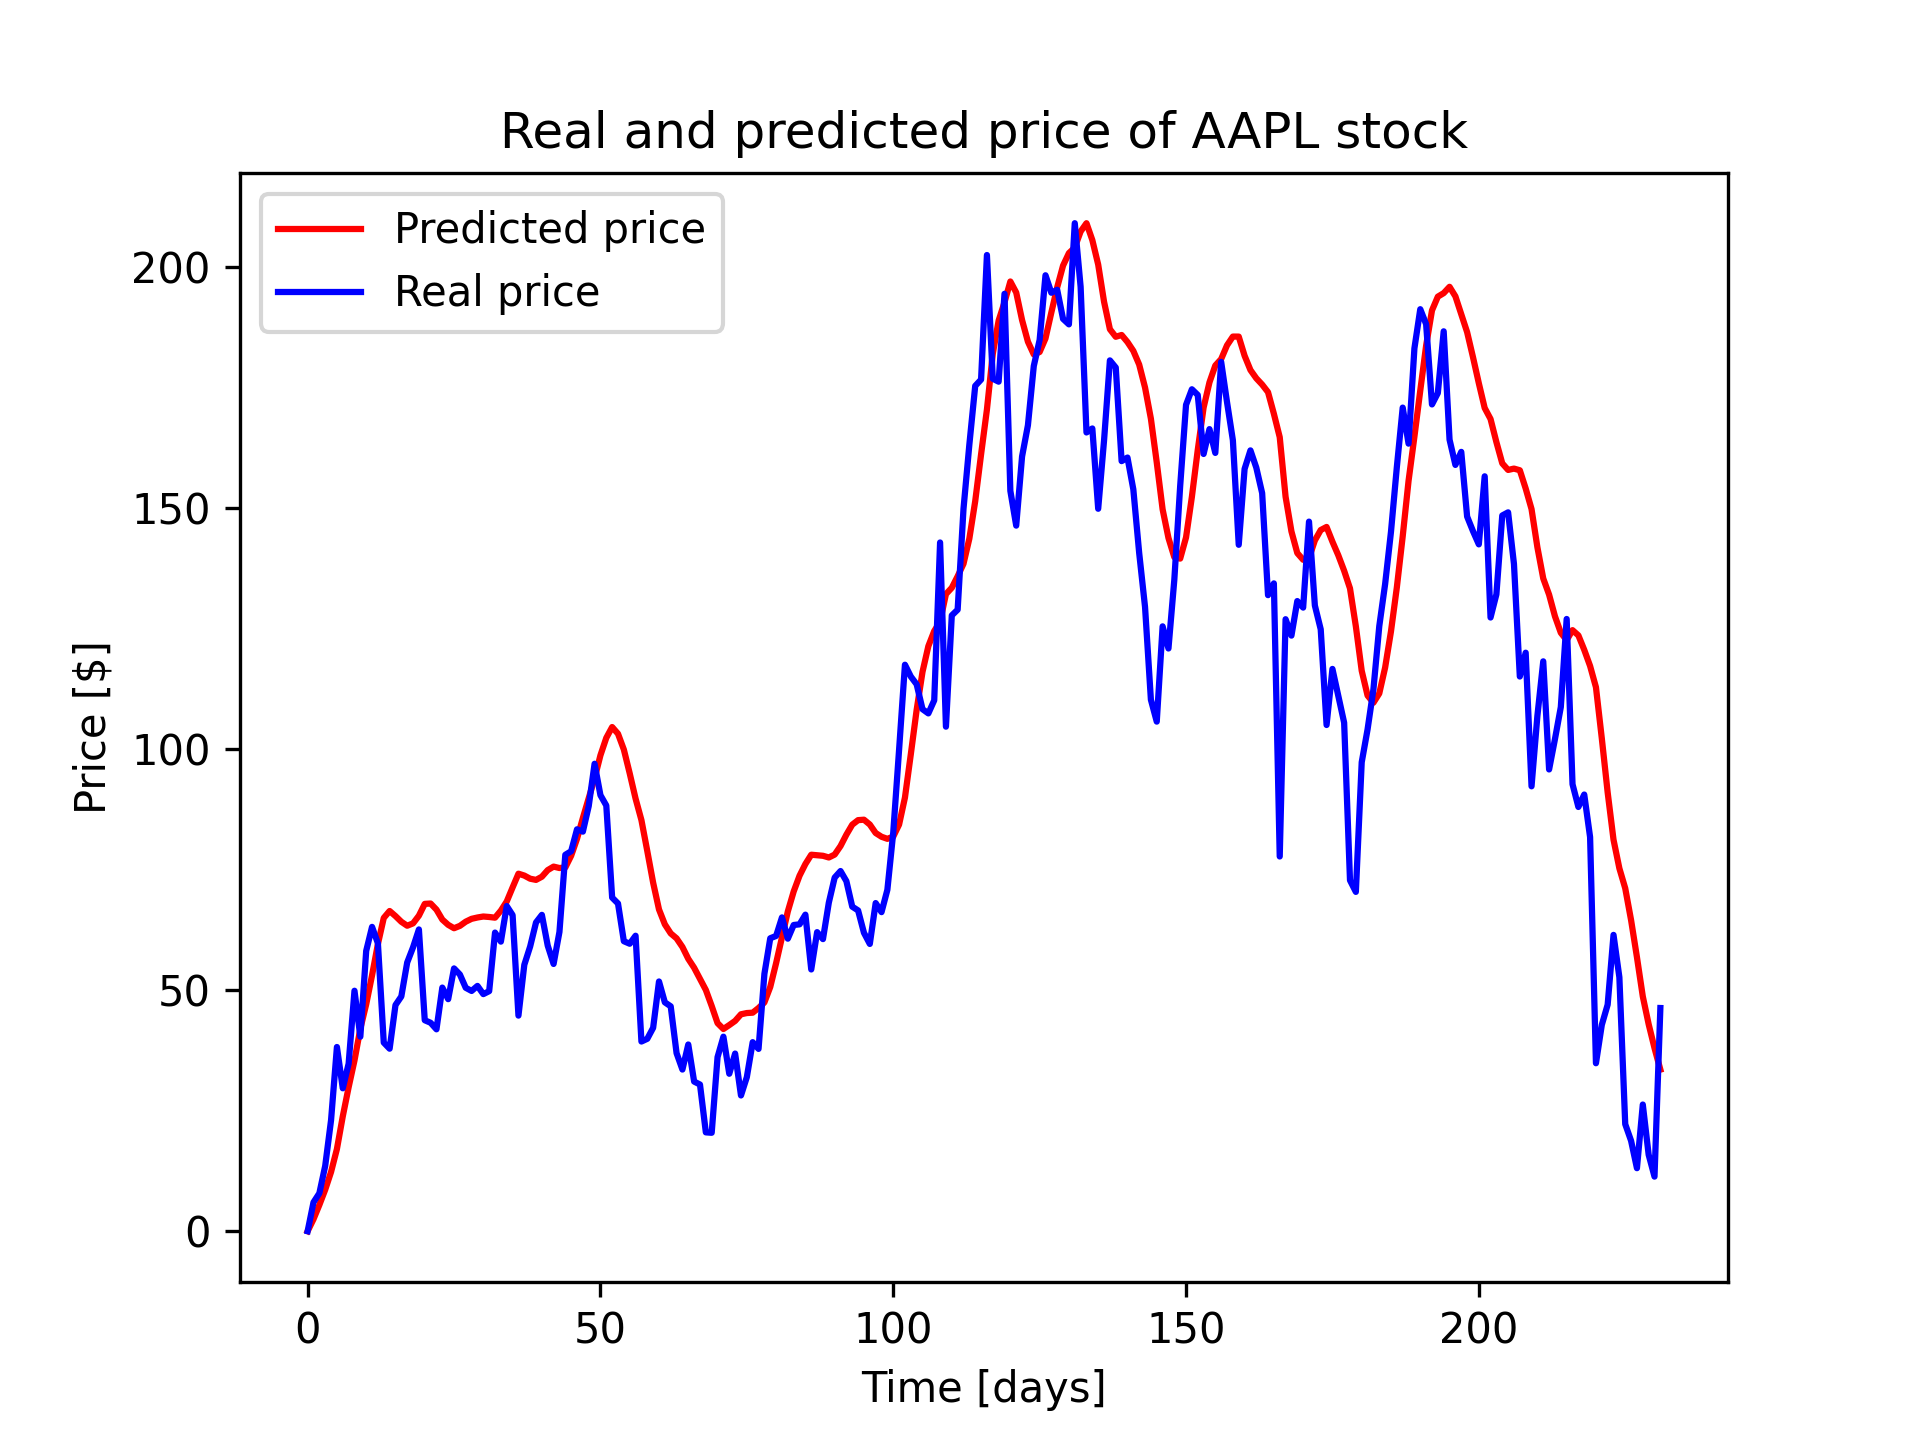
\includegraphics[width=0.5\textwidth]{./graf/model1/AAPL.png}
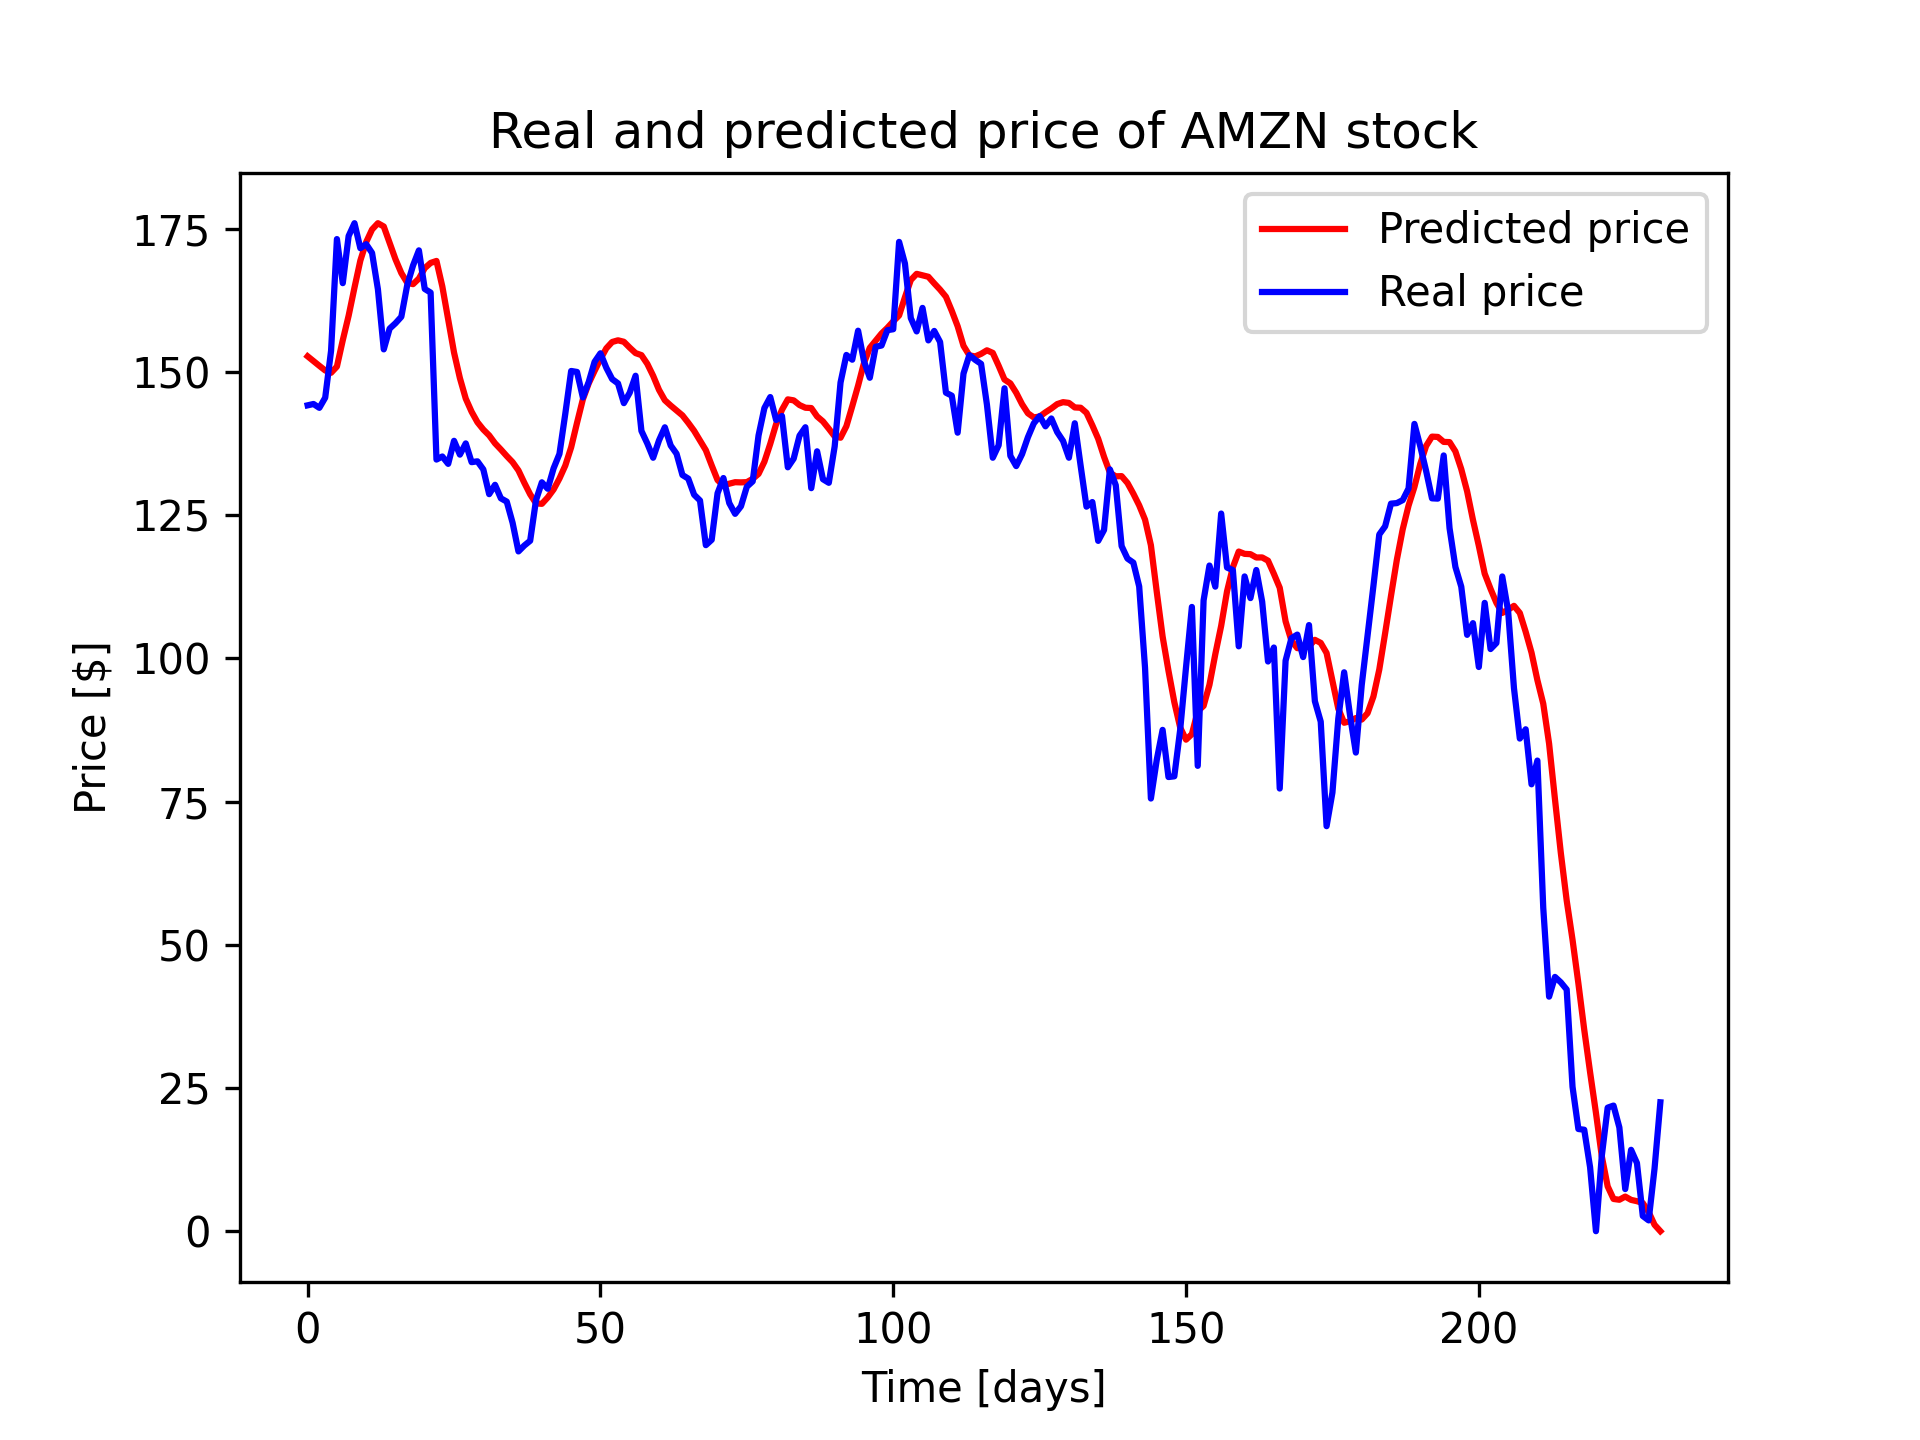
\includegraphics[width=0.5\textwidth]{./graf/model1/AMZN.png}
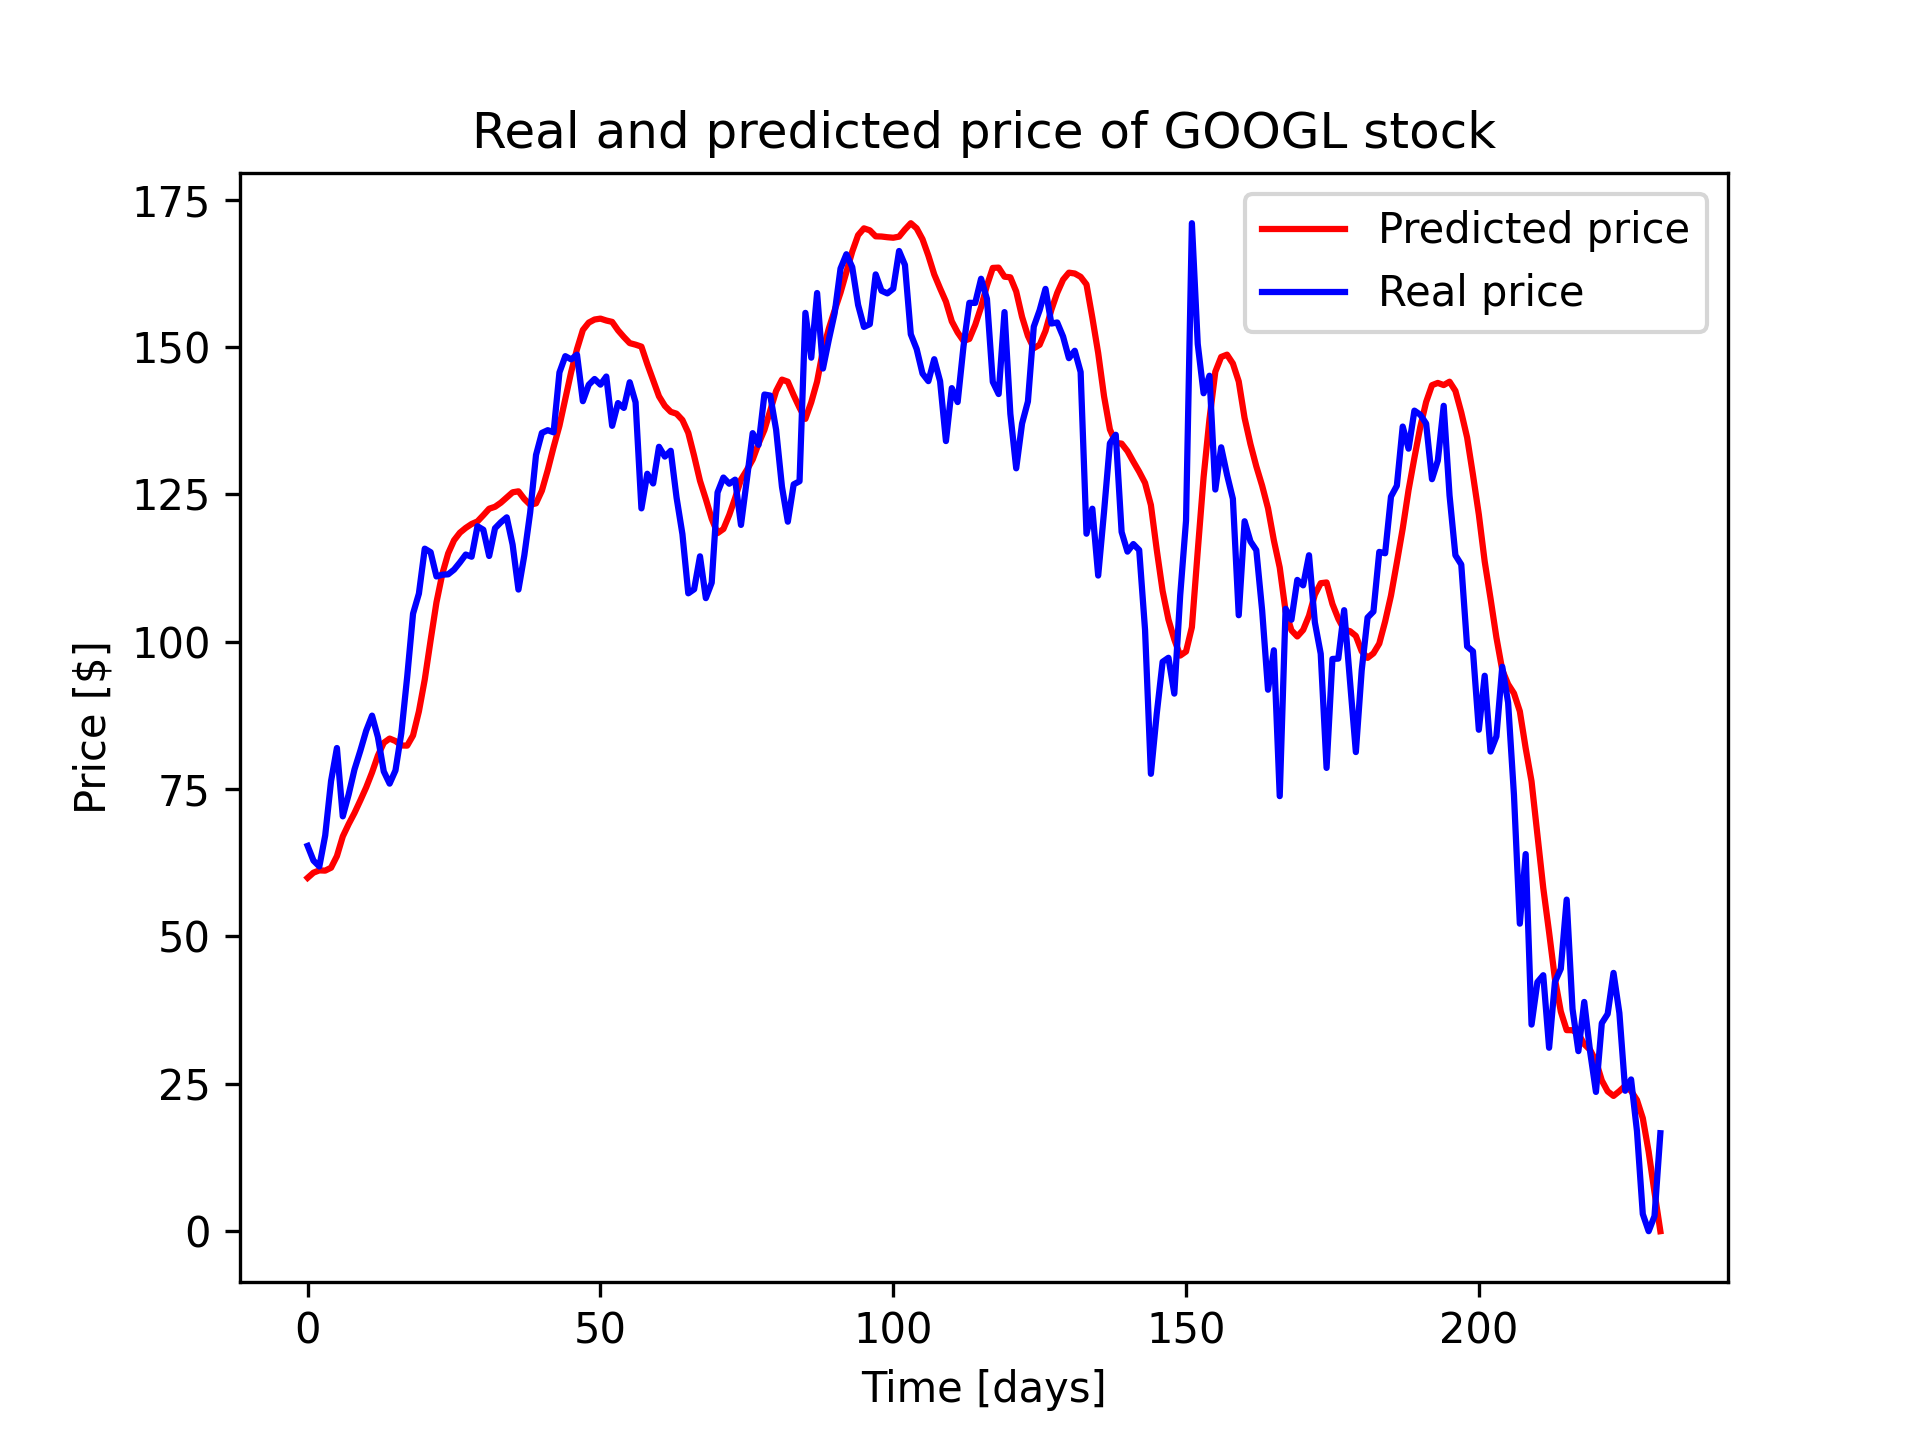
\includegraphics[width=0.5\textwidth]{./graf/model1/GOOGL.png}
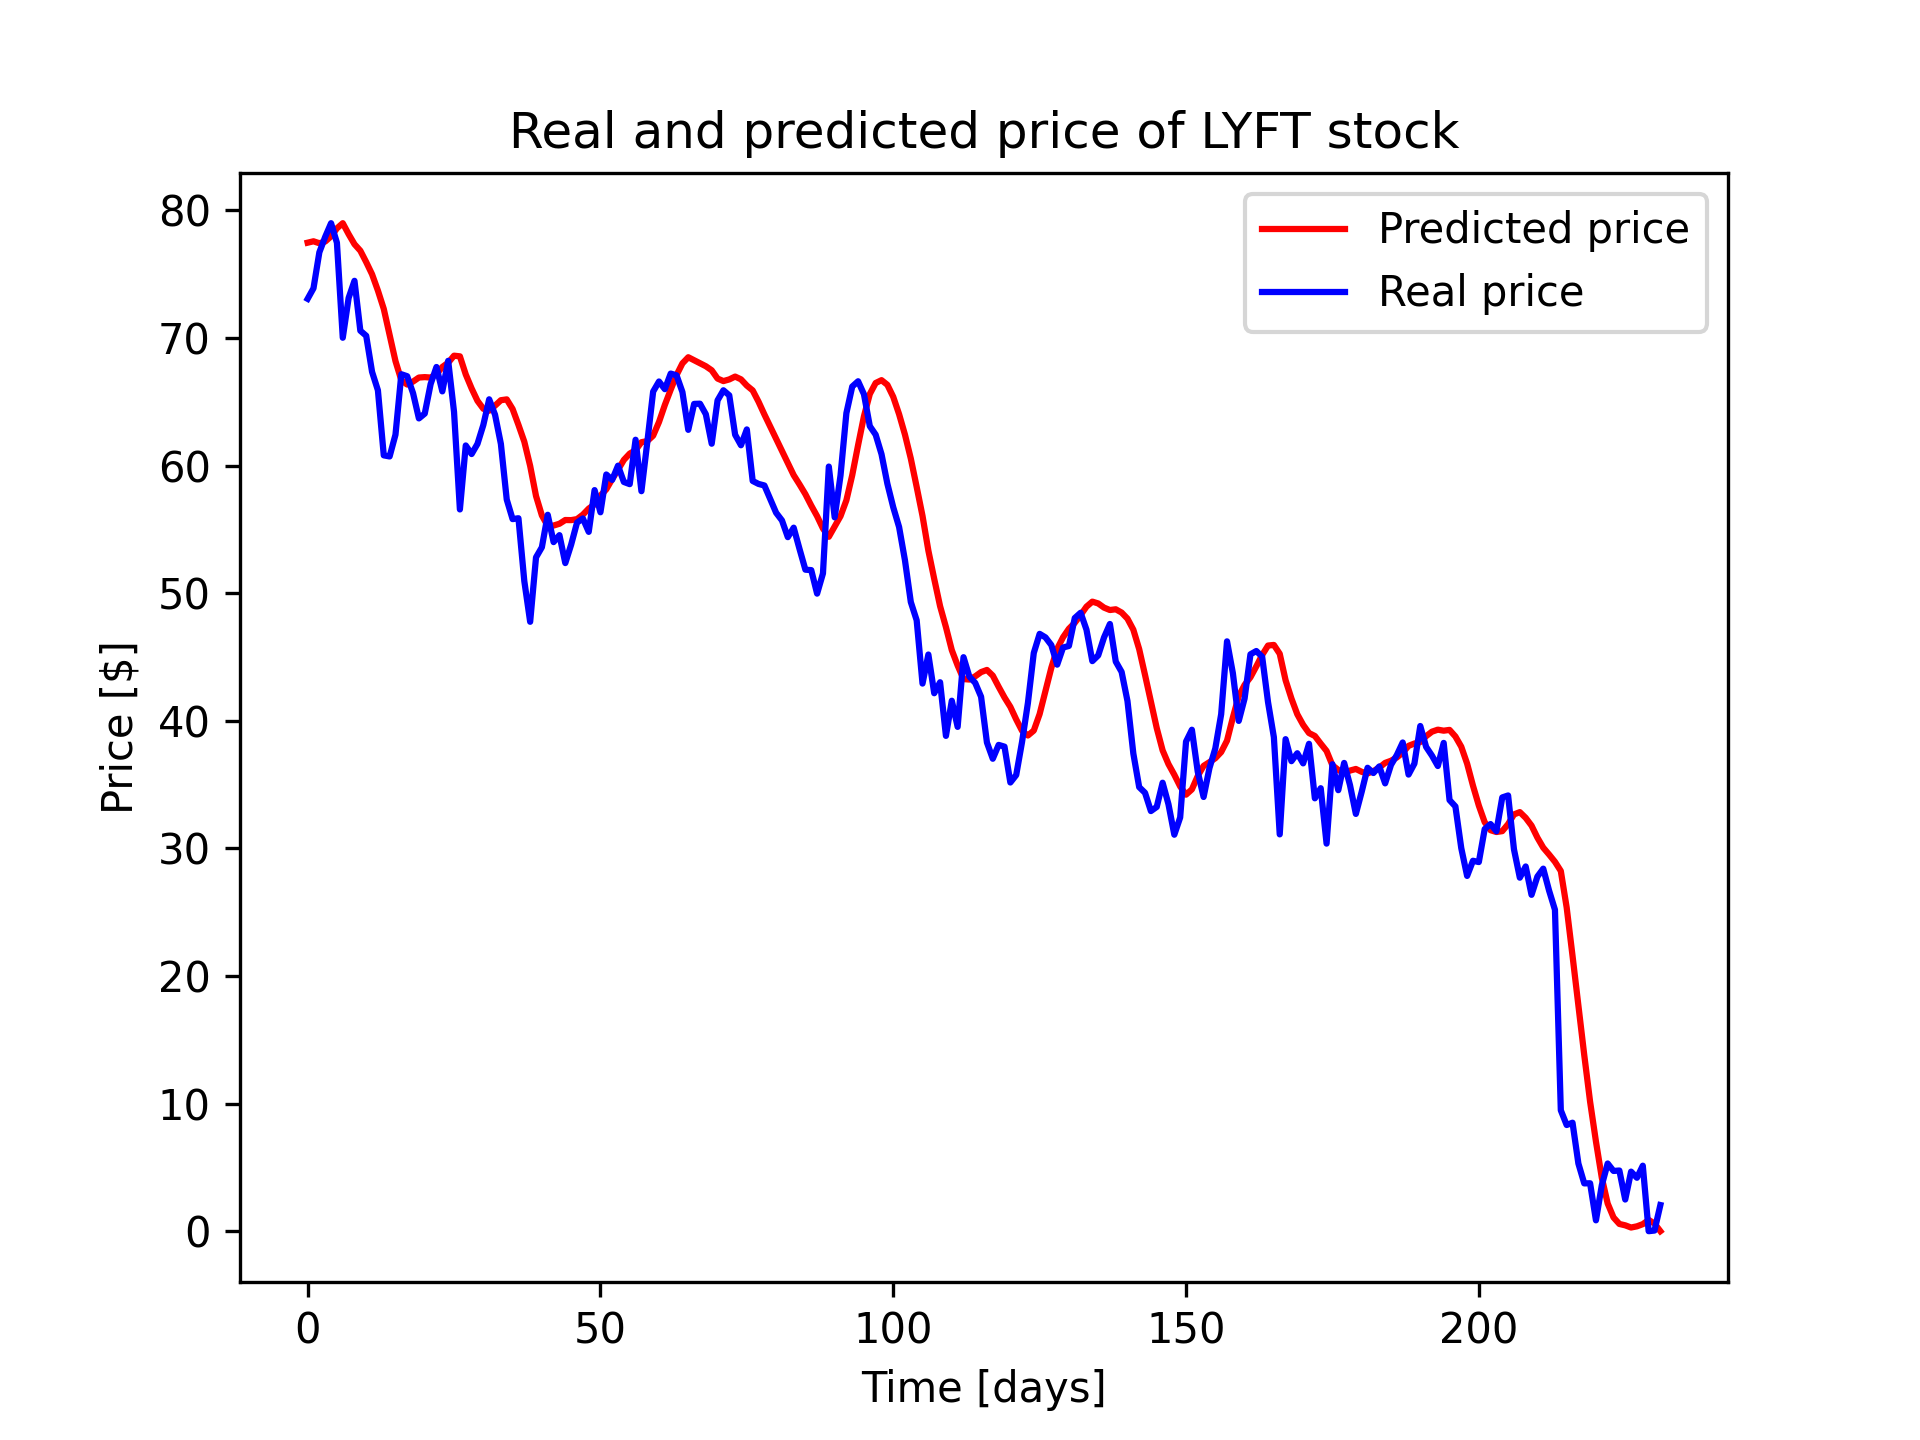
\includegraphics[width=0.5\textwidth]{./graf/model1/LYFT.png}
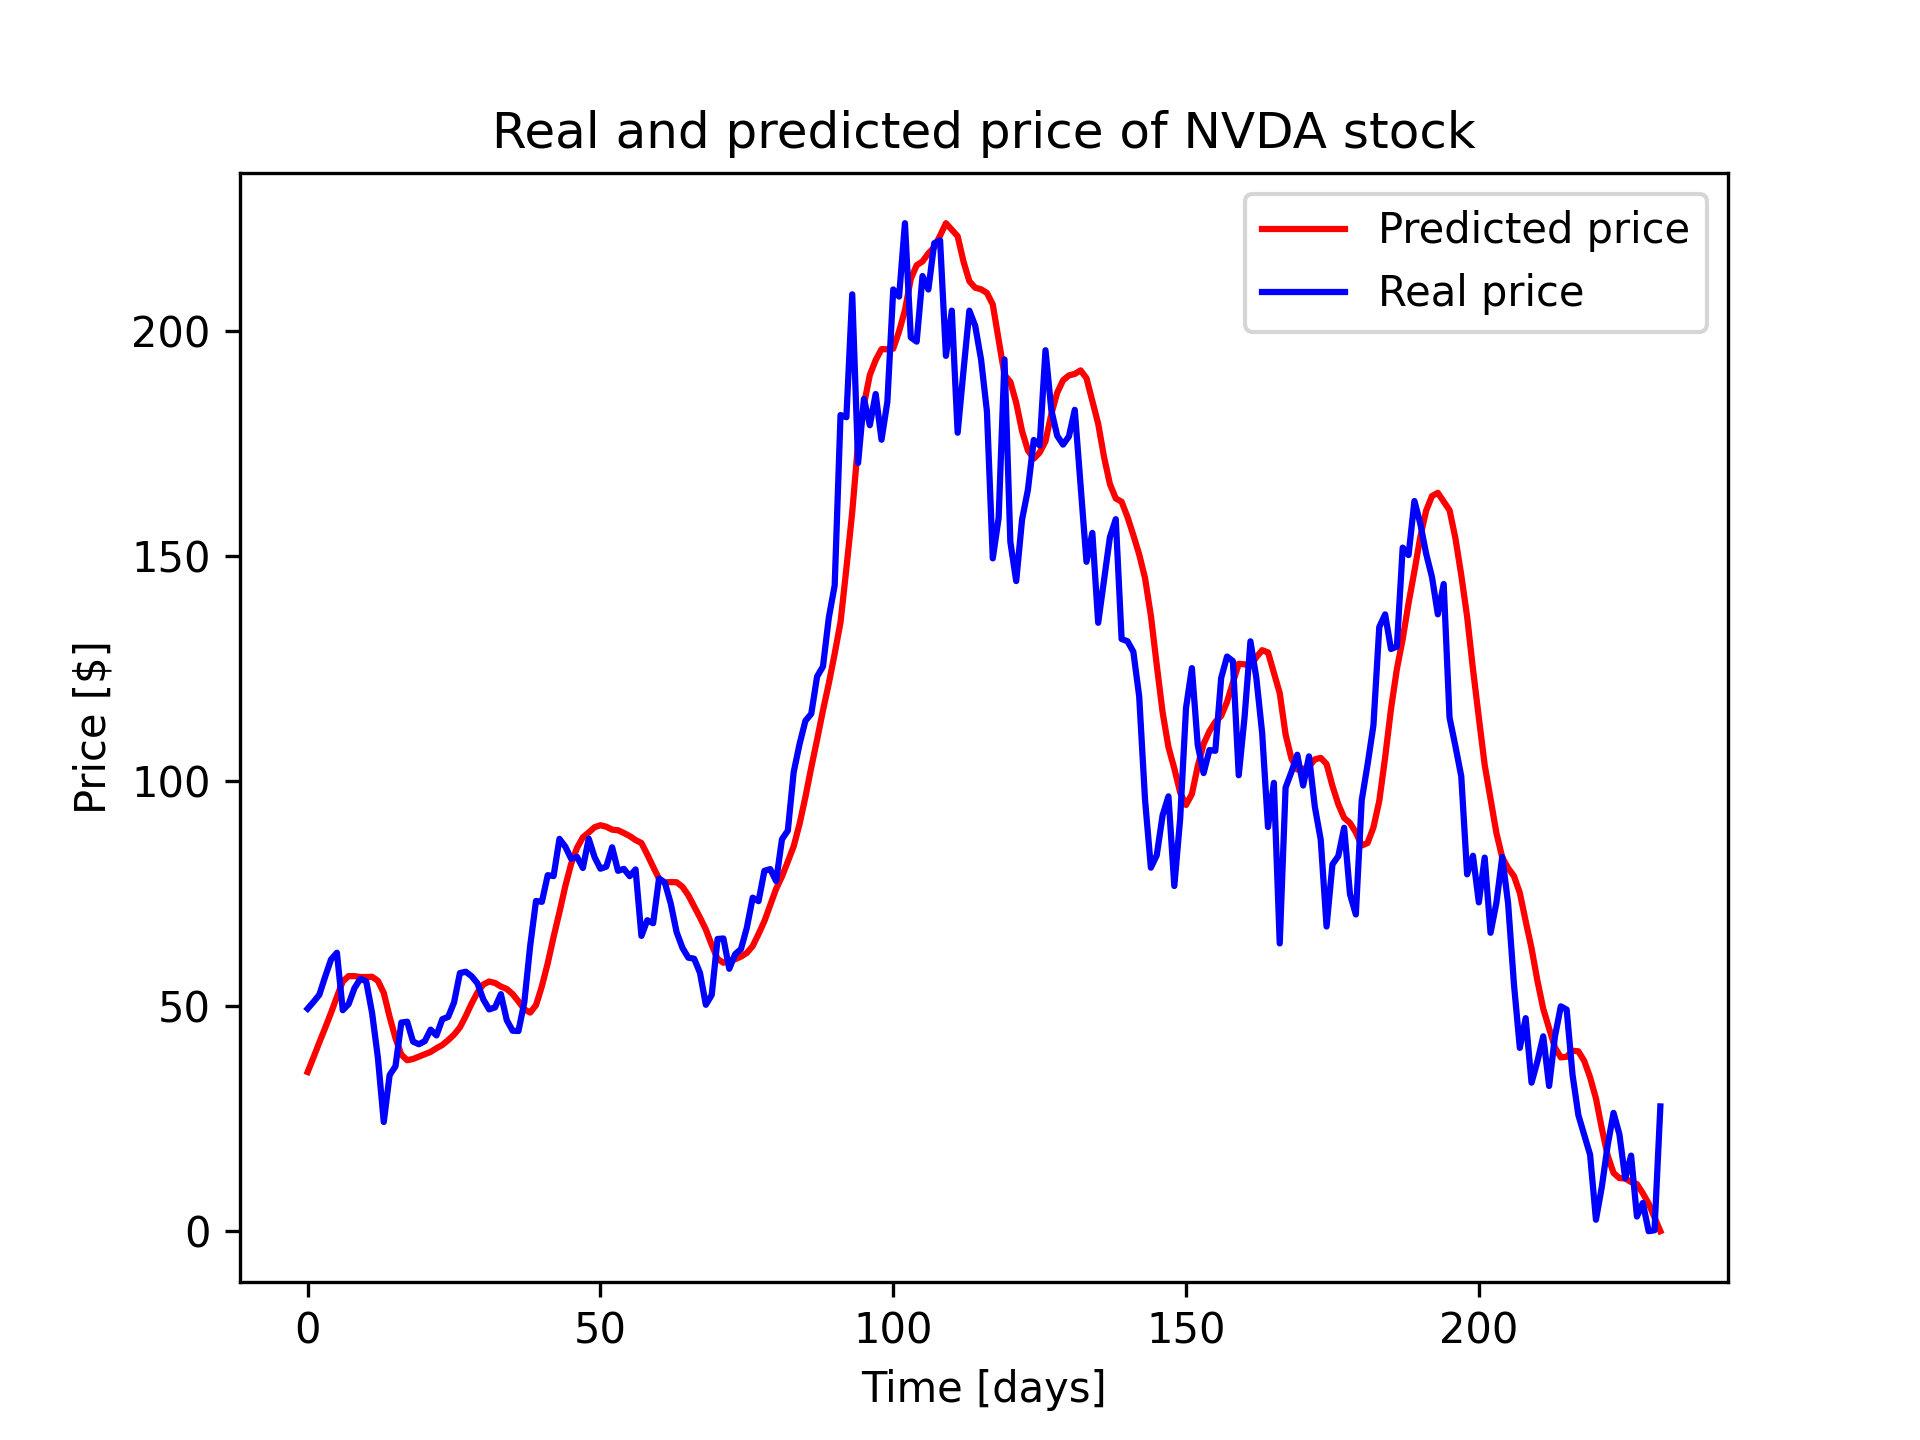
\includegraphics[width=0.5\textwidth]{./graf/model1/NVDA.png}
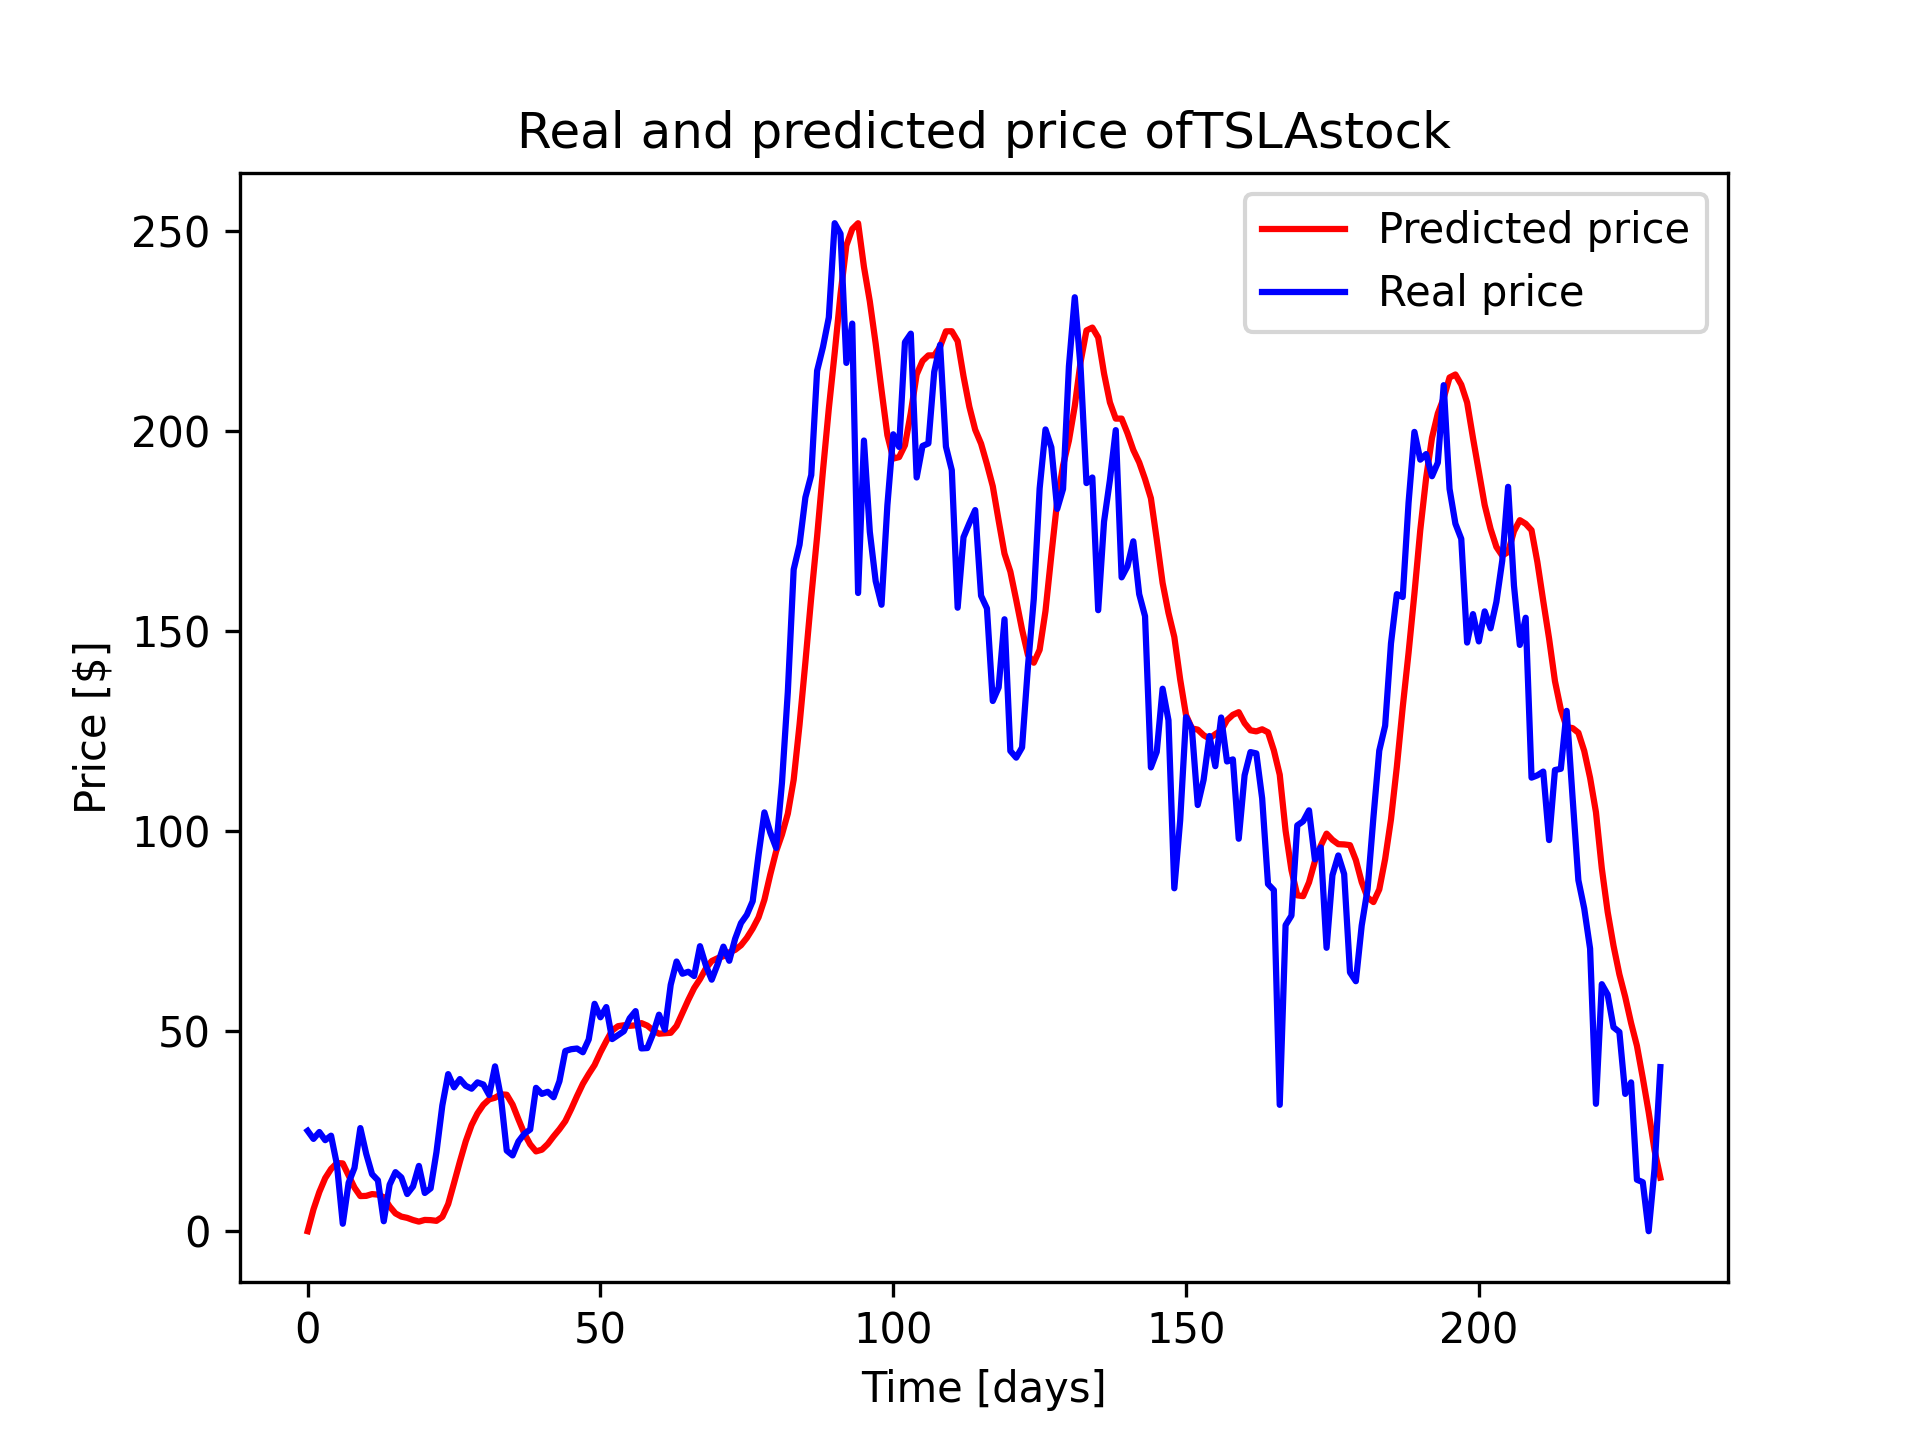
\includegraphics[width=0.5\textwidth]{./graf/model1/TSLA.png}
\caption{Real and predicted prices of the first model.}
\label{fig:label}
\end{figure} 

\clearpage
\subsection{Model 2}

Model2 - chunkSize: 20, time interval: 1 year, epochs: 10, trained on AAPL\par\bigskip
In model no. 2, it can be seen that the red line corresponding to the predicted price is slightly above
the blue line corresponding to the real price. It is worth noting that the peaks regarding the sudden
increase in the value of shares in both variants coincide. Sudden day-to-day swings are not included
in the red line, whether going up or down in the stock's value.
\par
Some anomalies, for example, sudden price spikes, are slightly delayed in the red line relative to the blue line.
Also, swift changes, for example, one-day large price fluctuations noticeable in the blue line, are invisible
in the red line.
\par\bigskip
loss: 0.008151059038937092\par
RMSE for AAPL equals 8.905762534366307\par
RMSE for AMZN equals 1.131803692397224\par
RMSE for GOOGL equals 6.083272264661717\par
RMSE for LYFT equals 2.0450747531362916\par
RMSE for NVDA equals 4.728504024706614\par
RMSE for TSLA equals 1.177903746100564\par


\begin{figure}
% \centering
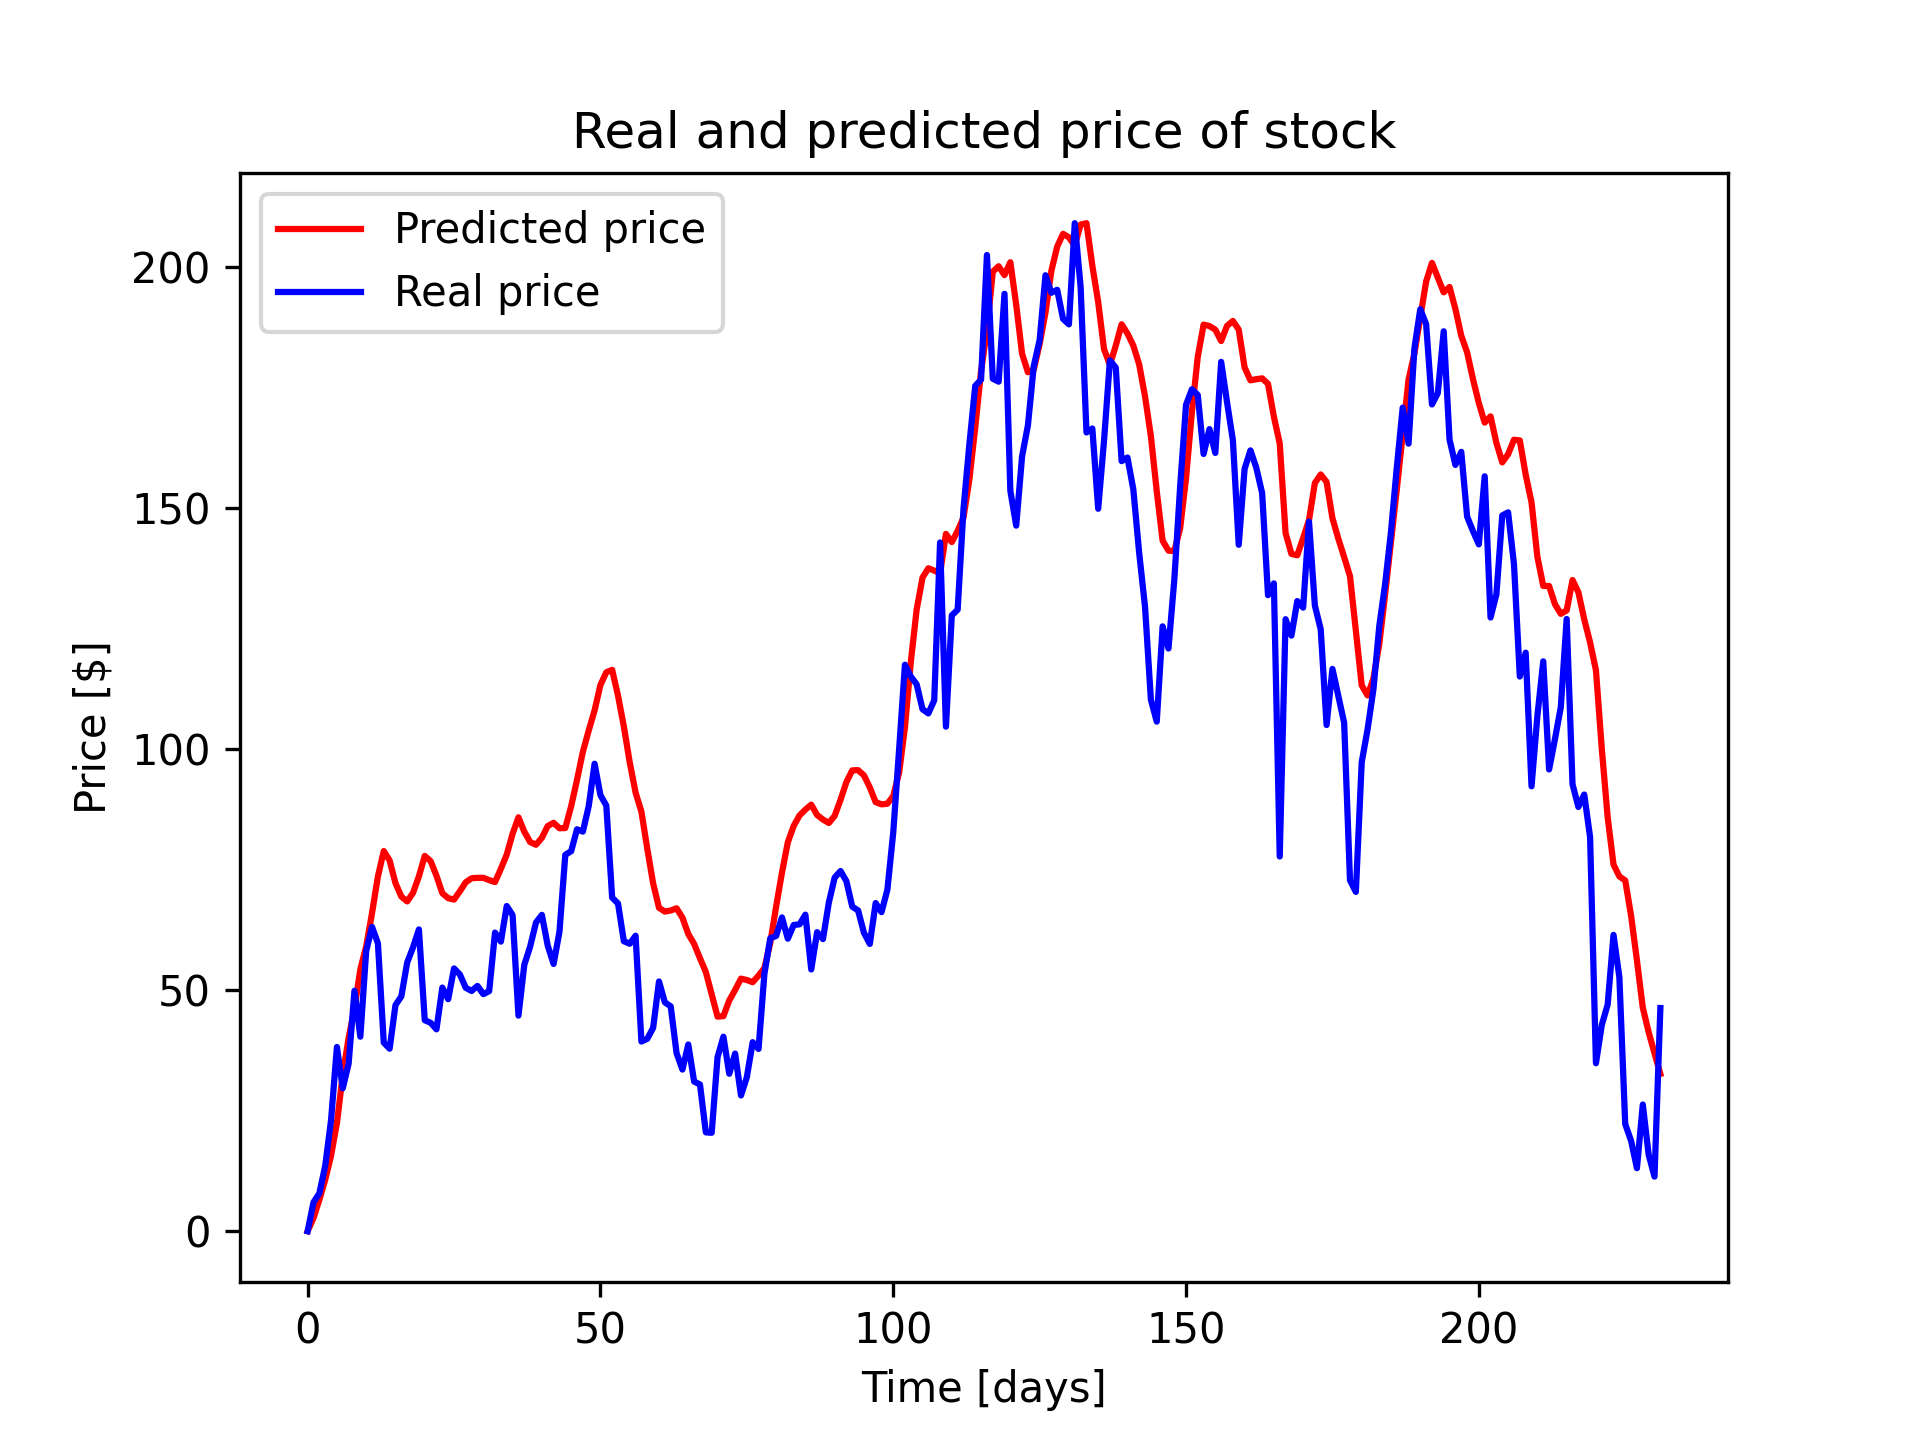
\includegraphics[width=0.5\textwidth]{./graf/model2/AAPL.png}
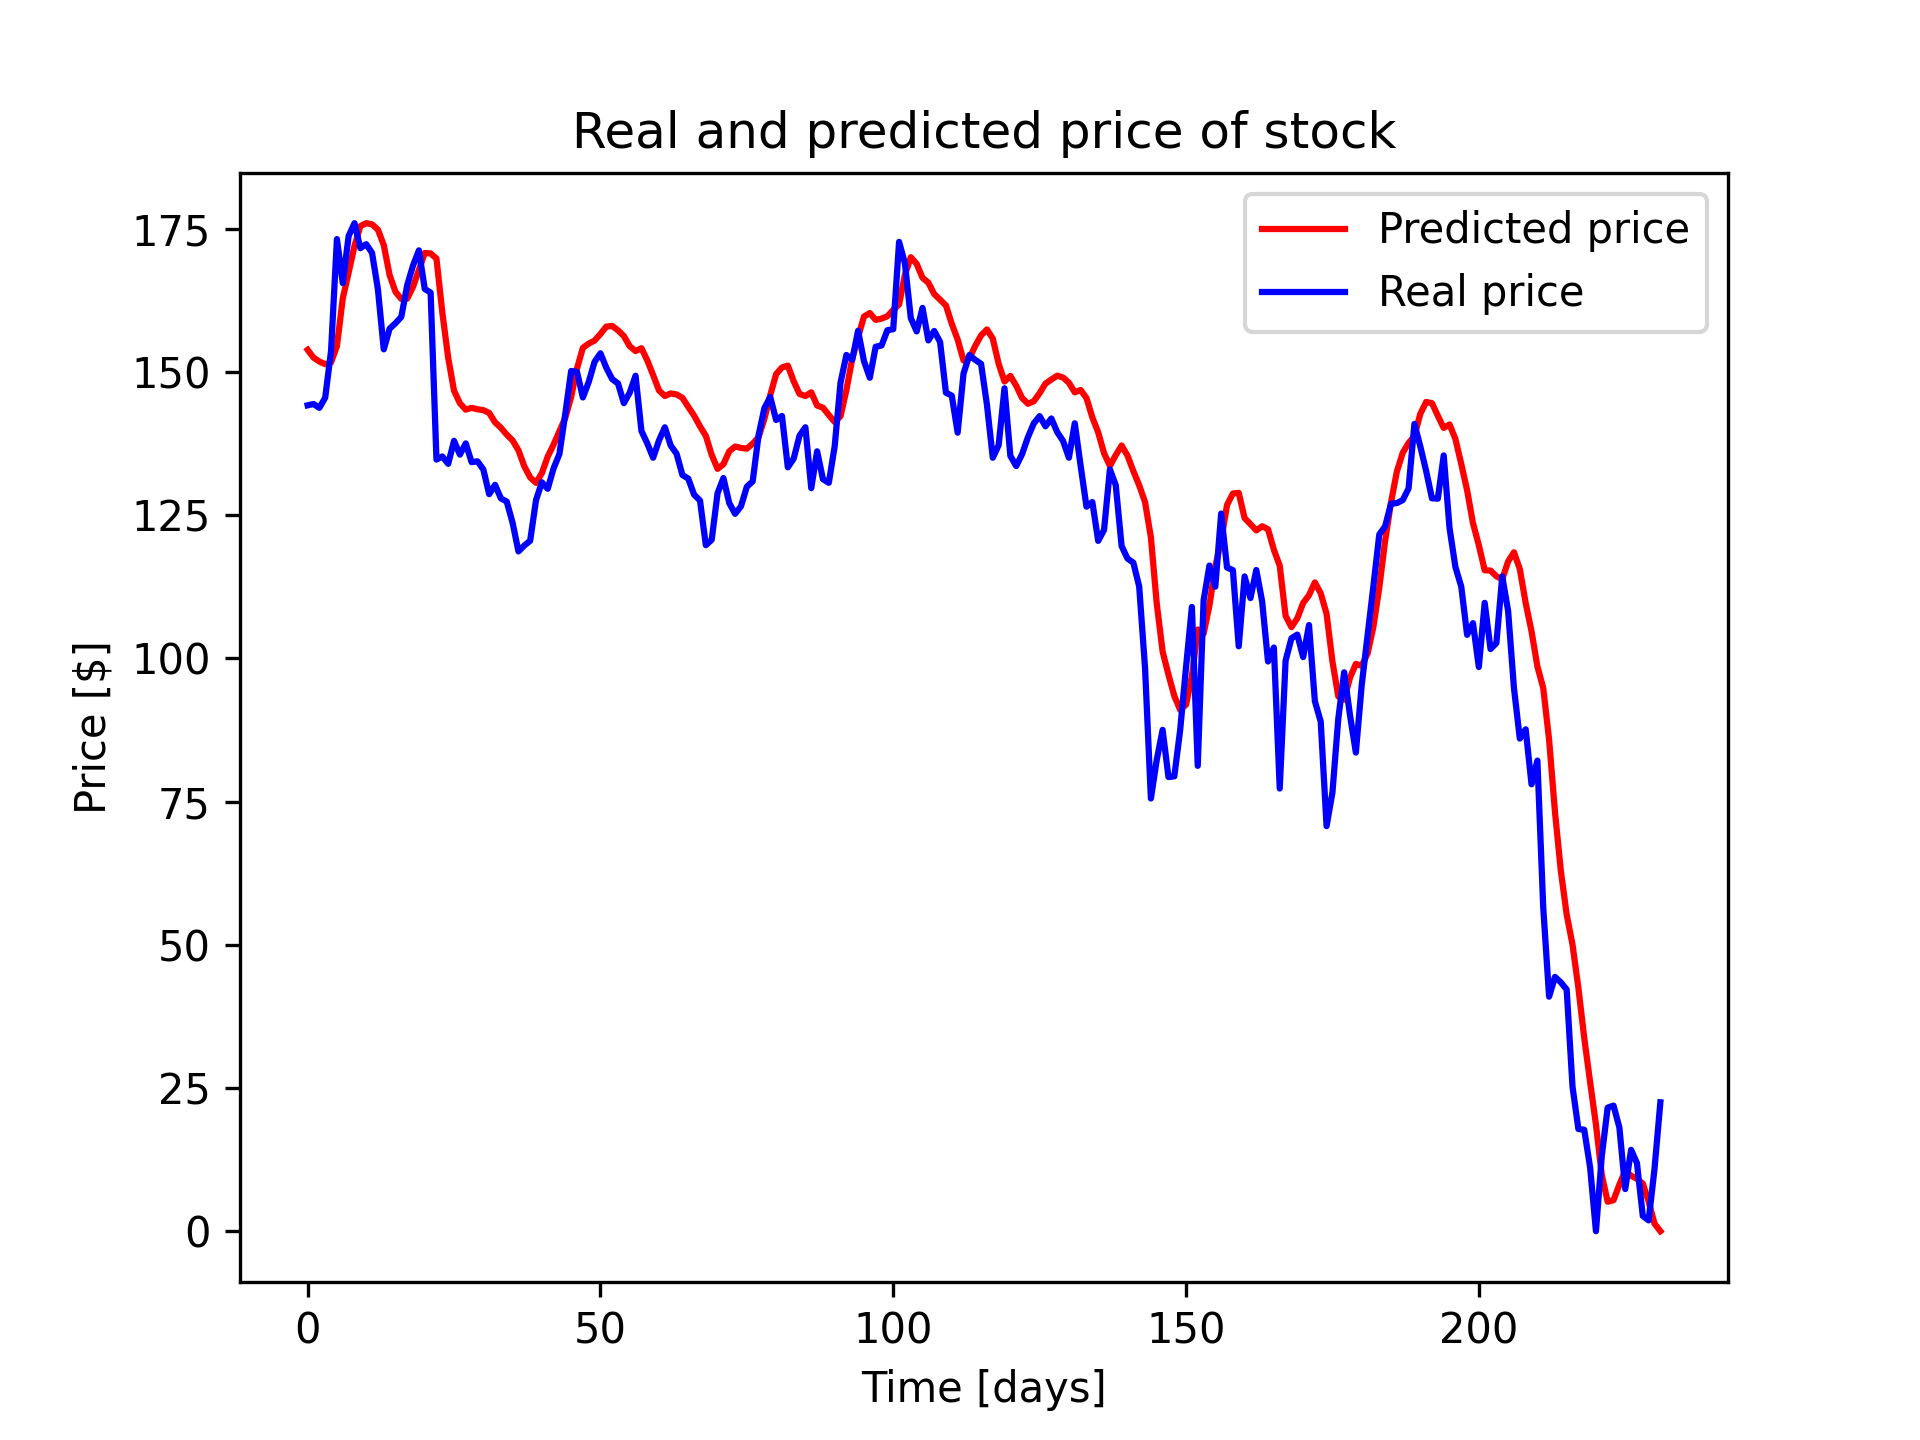
\includegraphics[width=0.5\textwidth]{./graf/model2/AMZN.png}
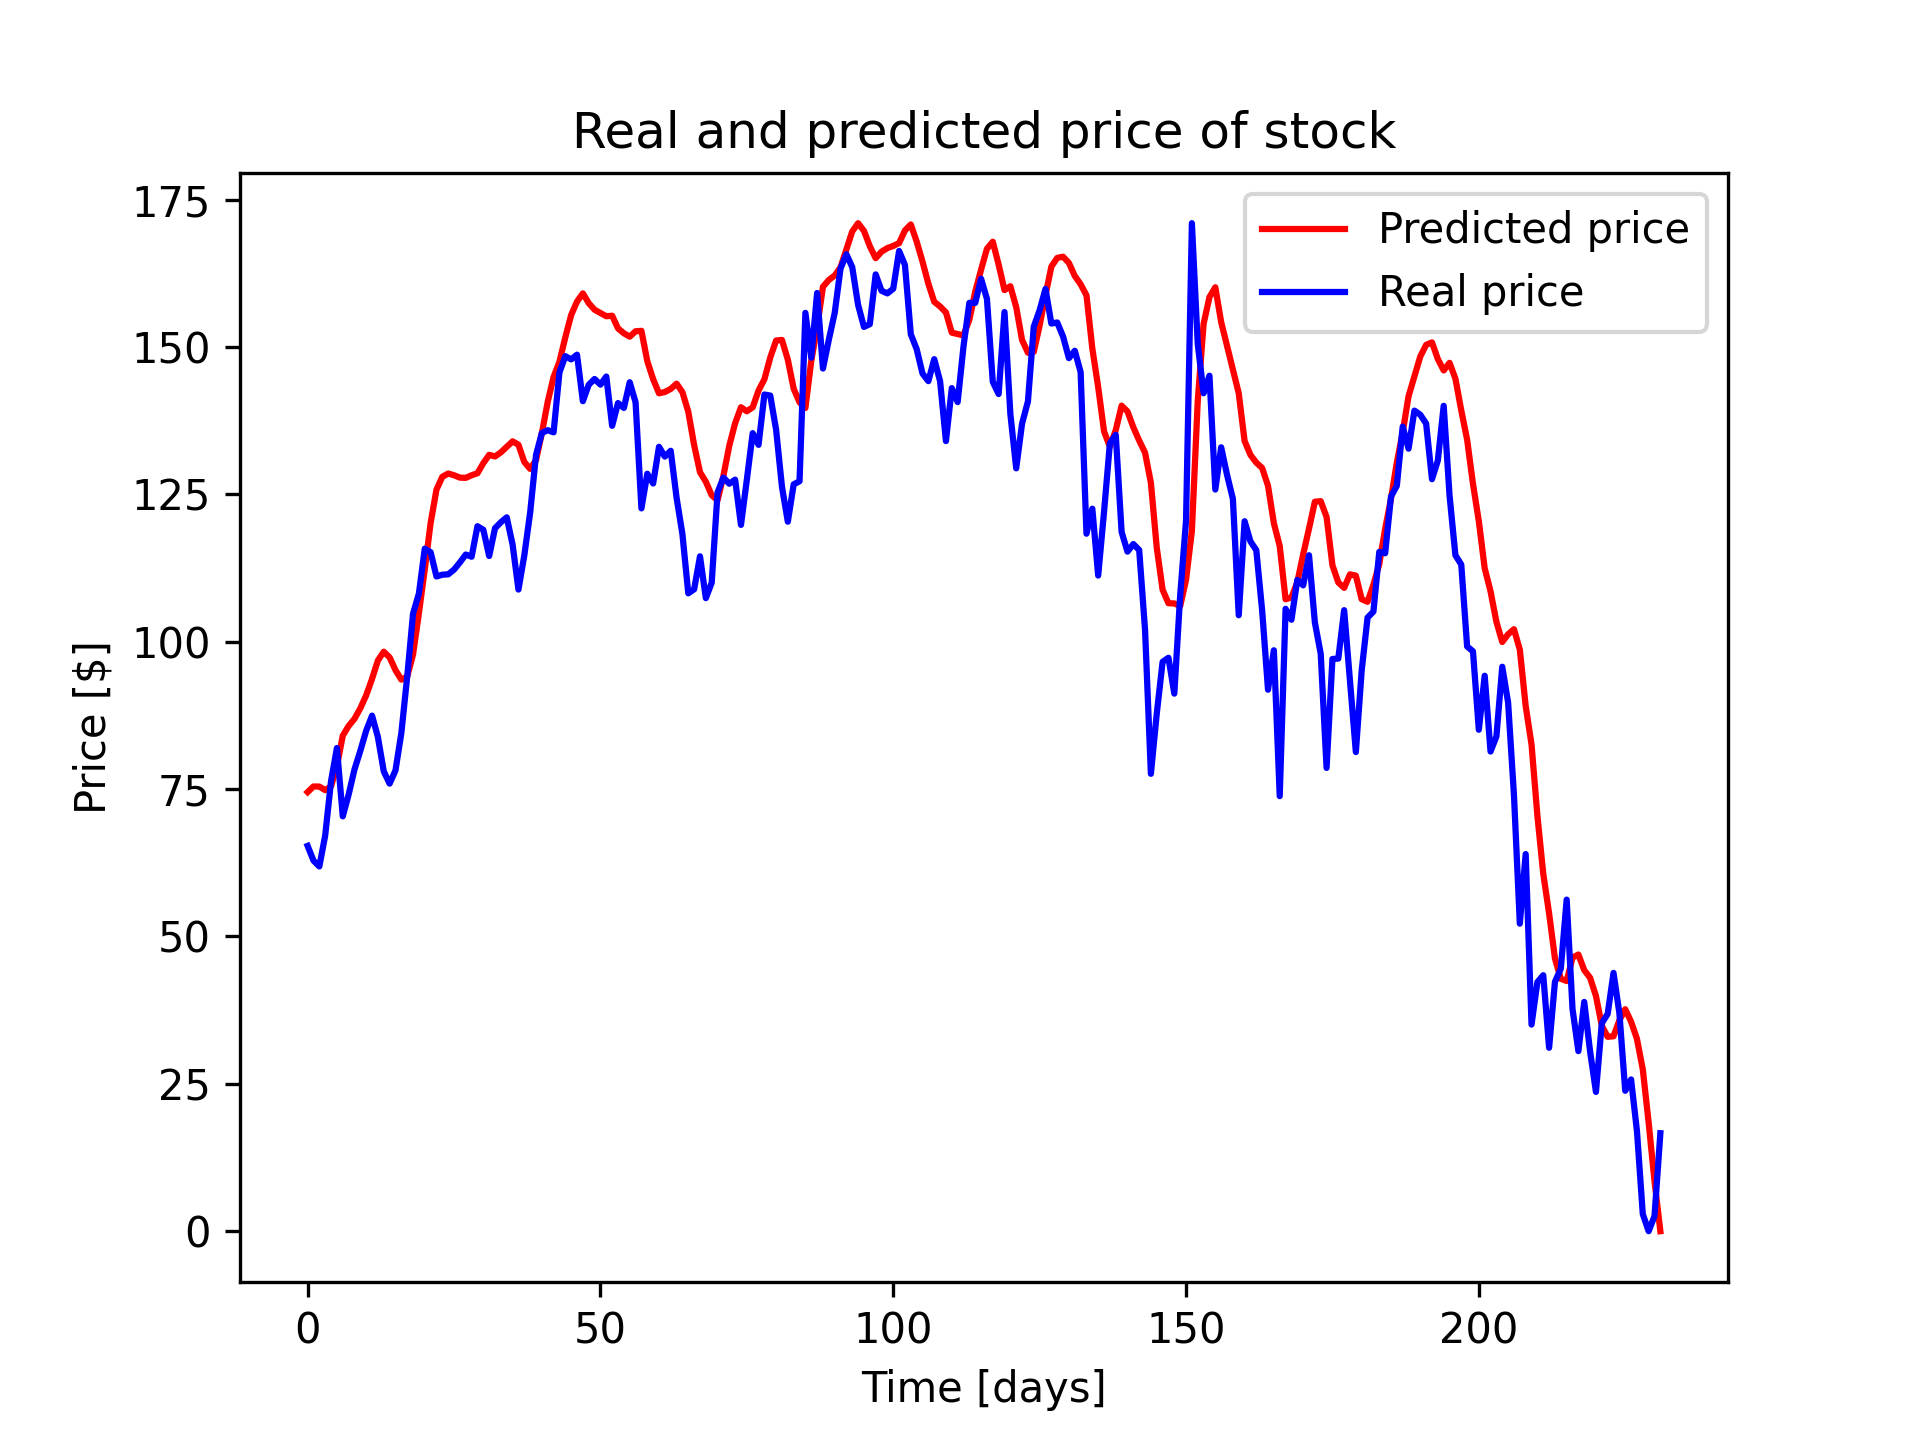
\includegraphics[width=0.5\textwidth]{./graf/model2/GOOGL.png}
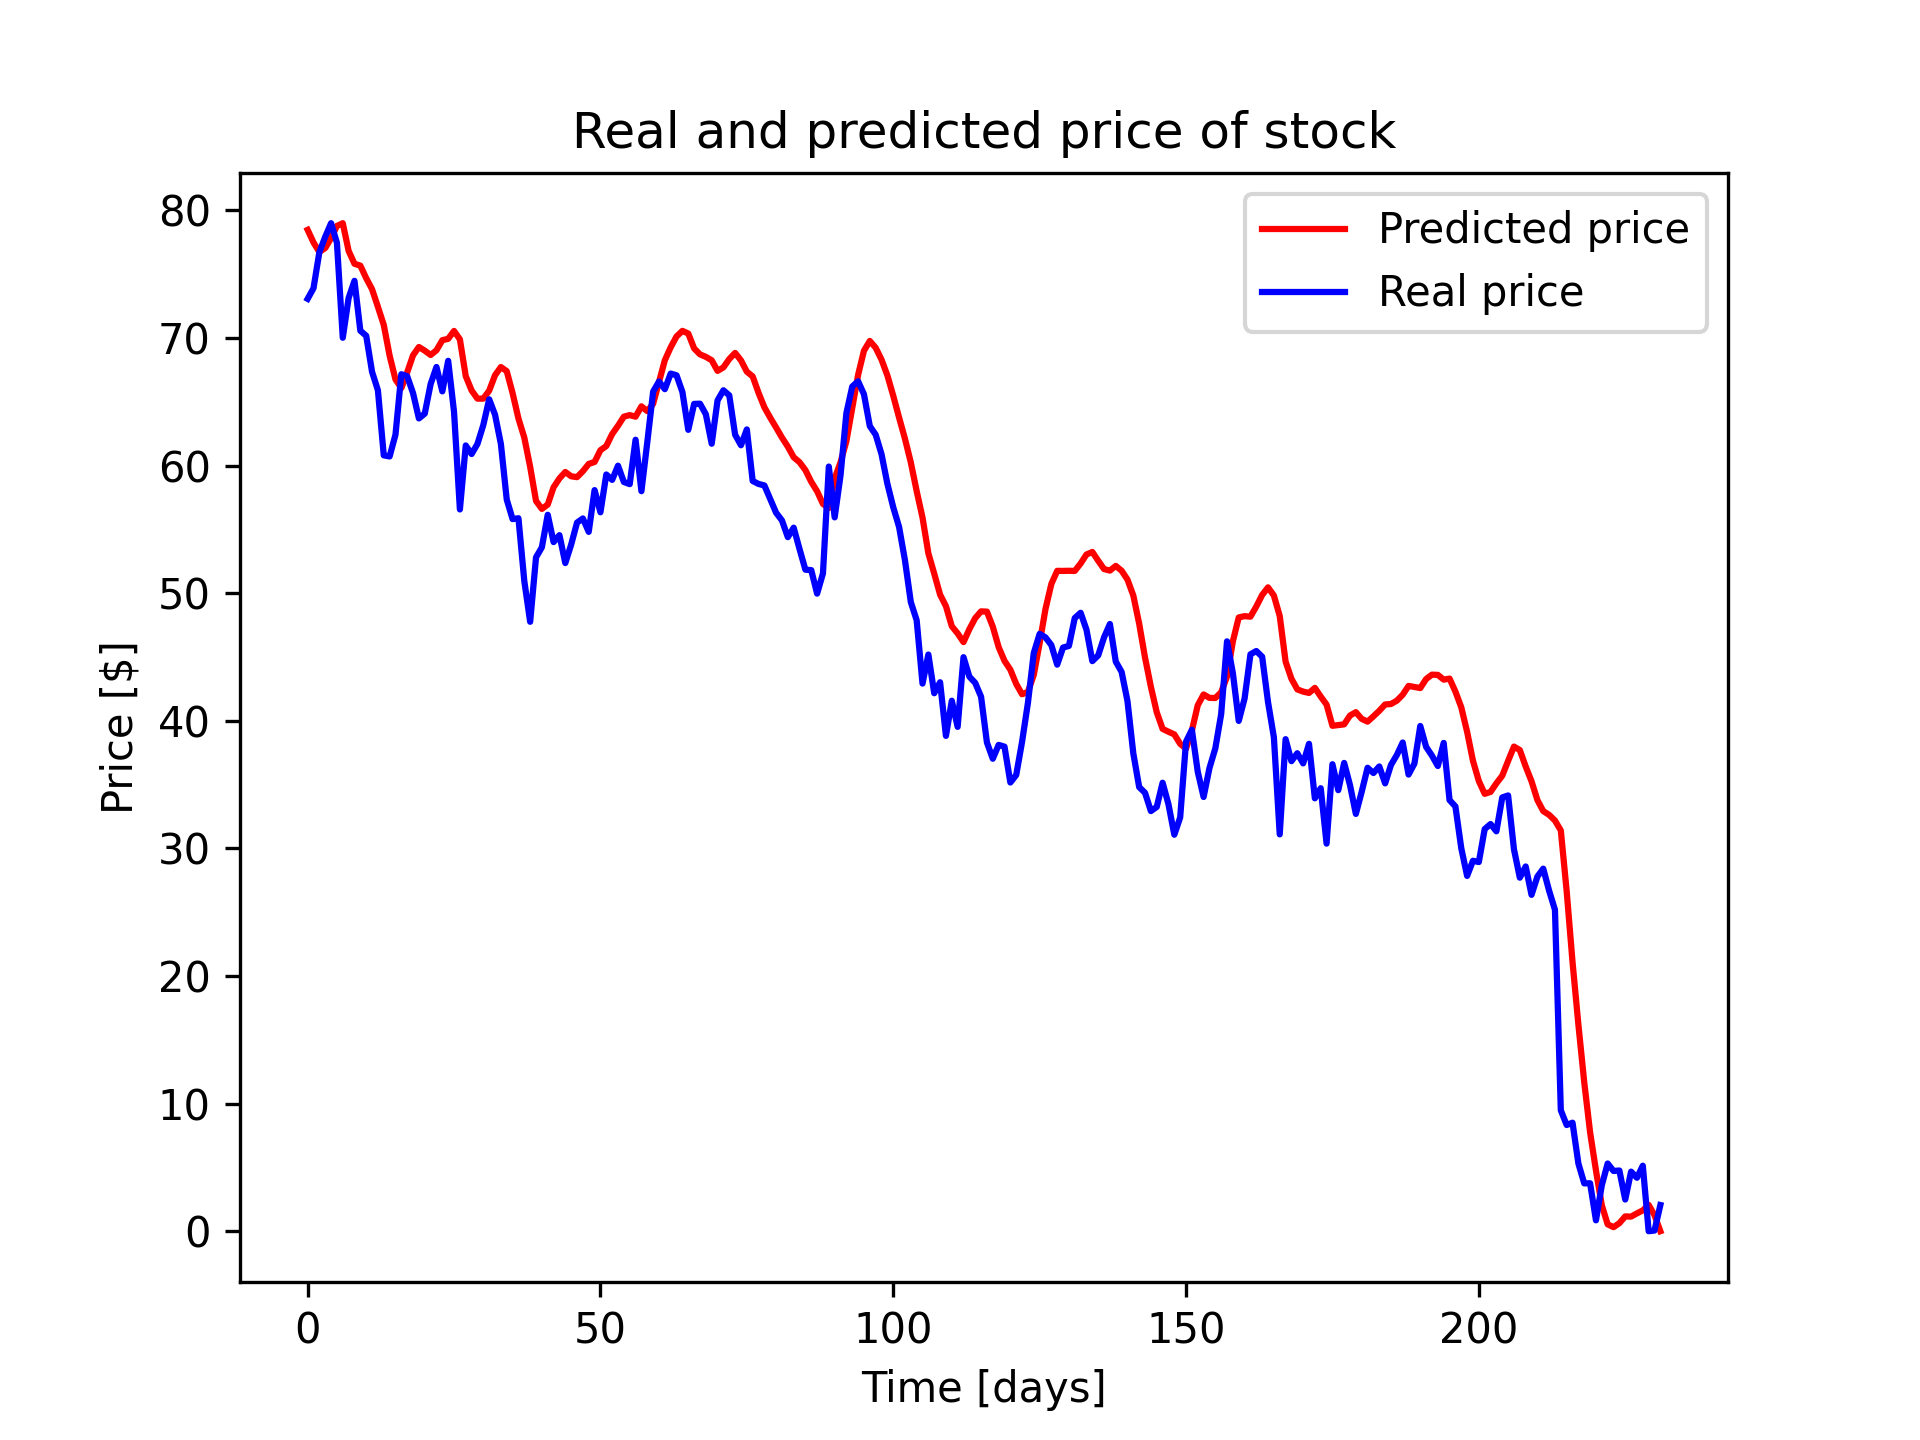
\includegraphics[width=0.5\textwidth]{./graf/model2/LYFT.png}
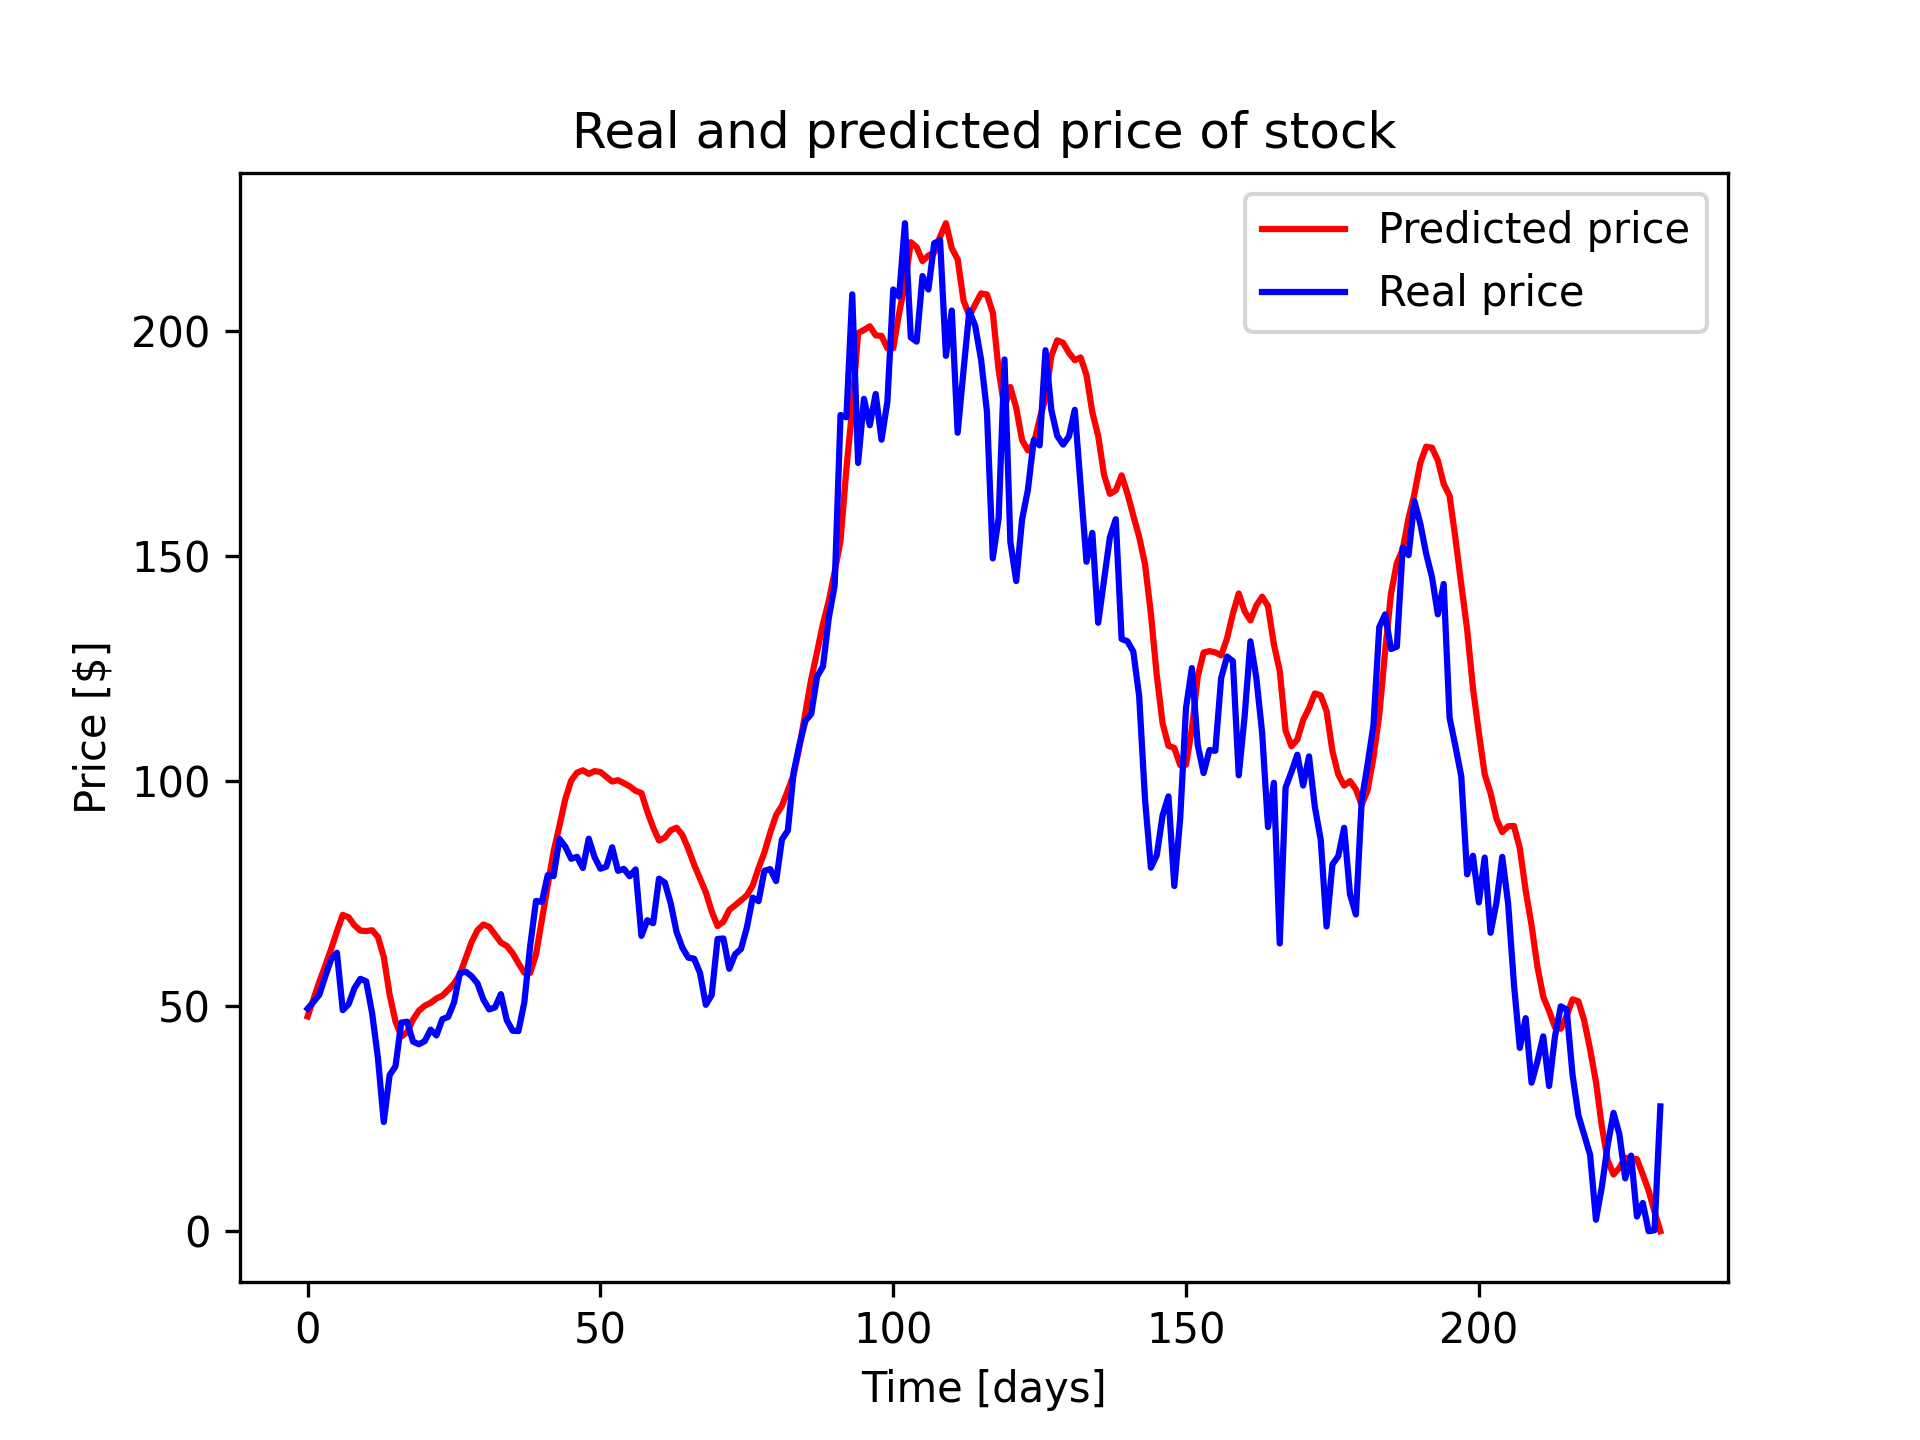
\includegraphics[width=0.5\textwidth]{./graf/model2/NVDA.png}
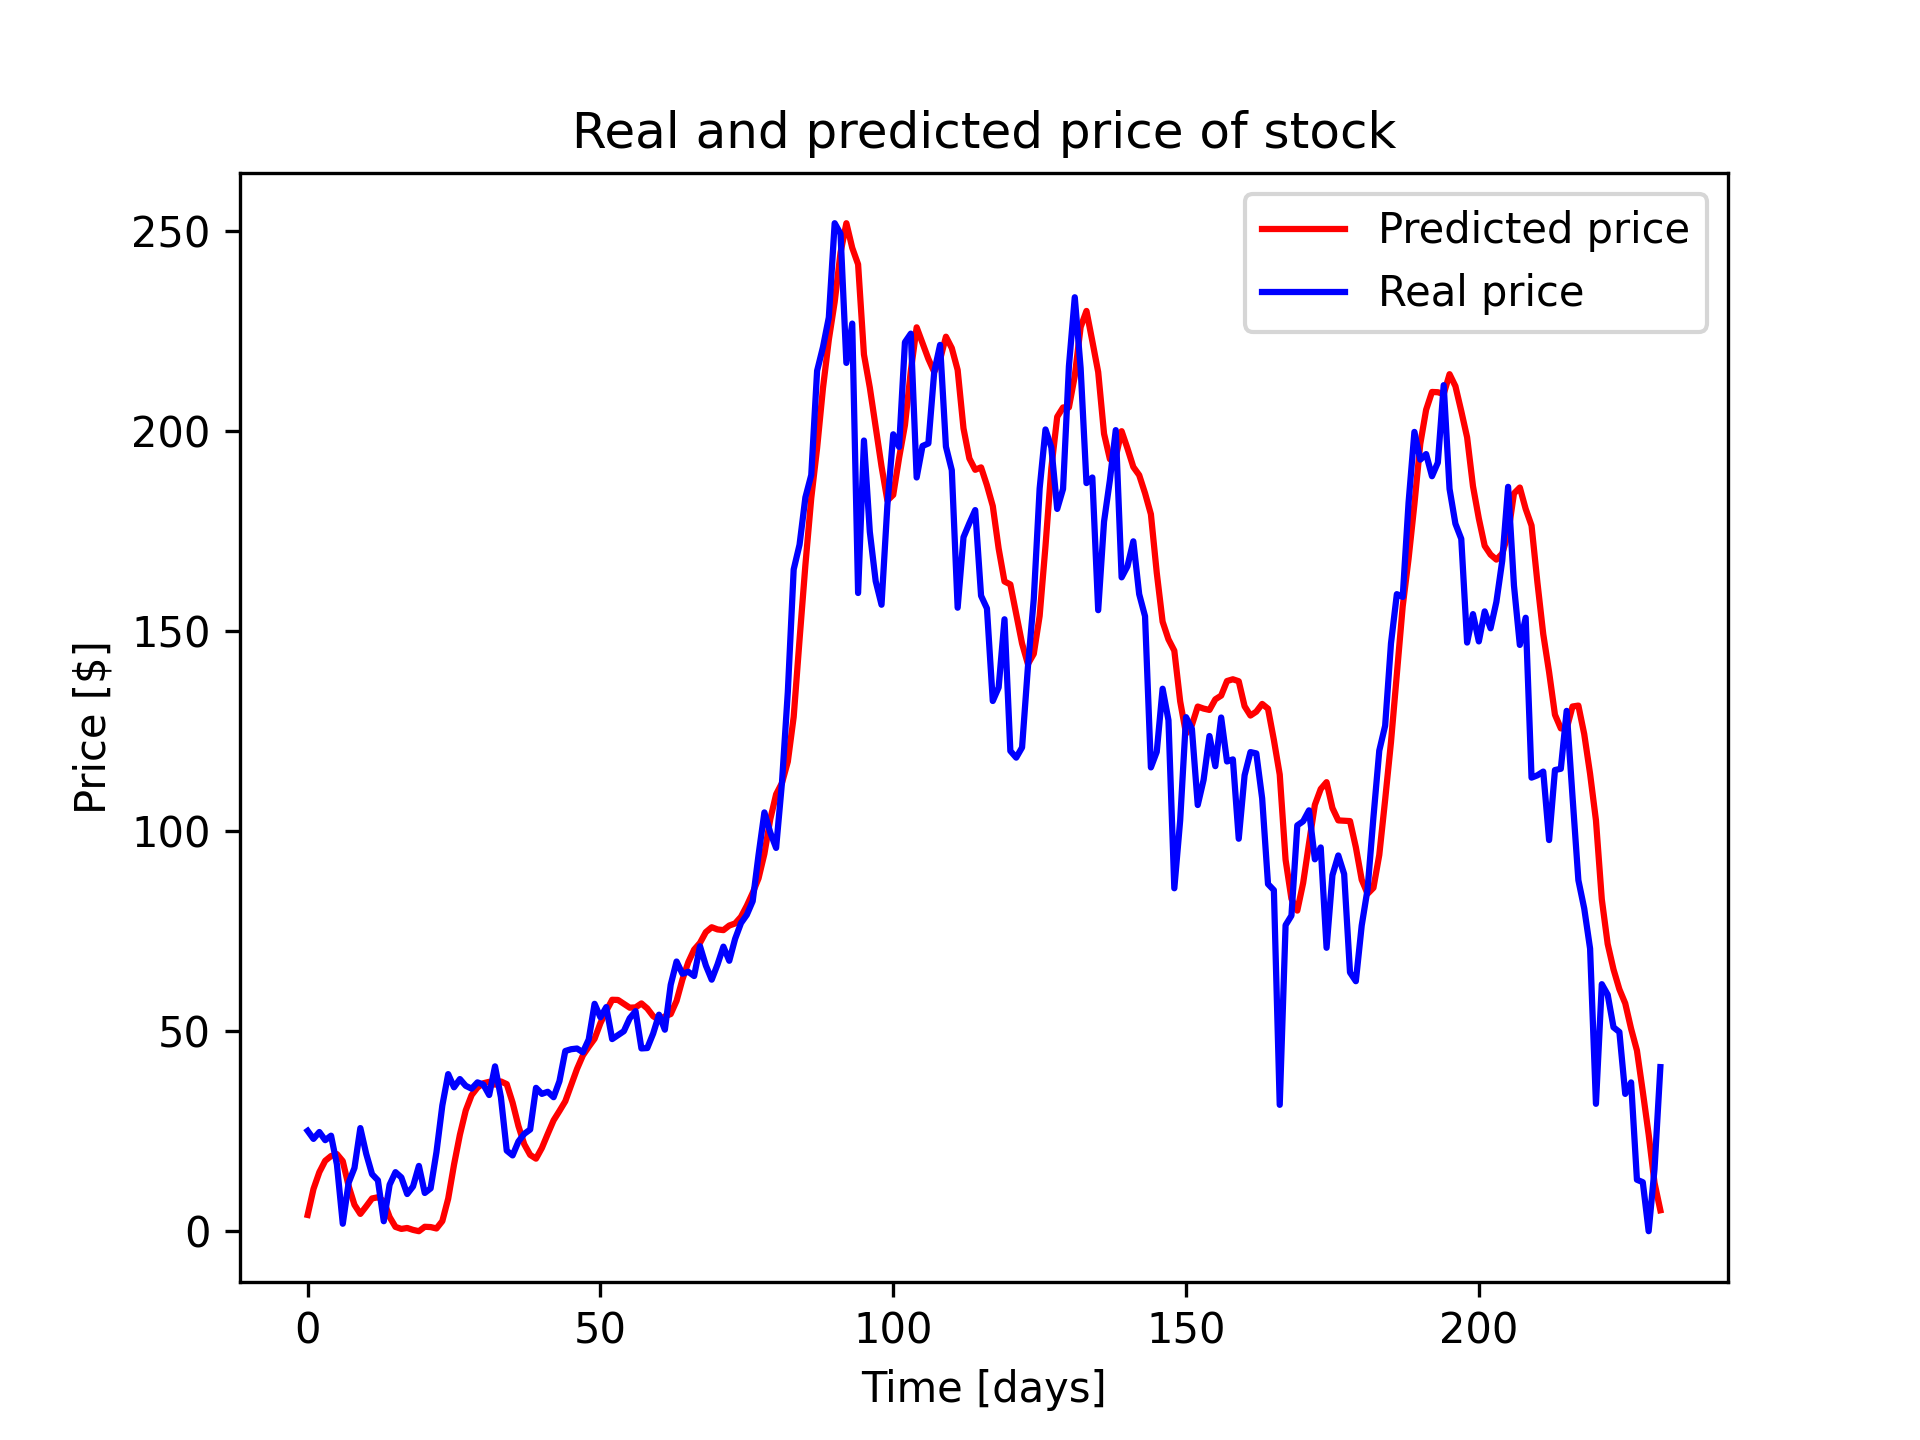
\includegraphics[width=0.5\textwidth]{./graf/model2/TSLA.png}
\caption{Real and predicted prices of the second model.}
\label{fig:label}
\end{figure} 

\clearpage
\subsection{Model 3}

Model3 - chunkSize: 20, time interval: 1 year, epochs: 15, trained on AAPL\par\bigskip
In the next model, at first glance, both lines almost coincide. After a careful analysis of the charts,
however, it can be seen that in some cases, the predicted price is slightly overestimated concerning
the real price. Some charts show that the predicted price is {\$}5 higher than the real price.
There are also visible lags of several days between the expected and real prices. In four plots
of this model (AAPL.png, GOOGL.png, NVDA.png, TSLA.png), it was observed that significant and
sudden amplitudes were not included in the sine of the red line.
\par\bigskip
loss: 0.0052094003185629845\par
RMSE for AAPL equals 10.383642993259755\par
RMSE for AMZN equals 2.185266997776006\par
RMSE for GOOGL equals 7.797997029403418\par
RMSE for LYFT equals 2.3010552912763744\par
RMSE for NVDA equals 6.124846943497234\par
RMSE for TSLA equals 1.1923880490956362\par


\begin{figure}
% \centering
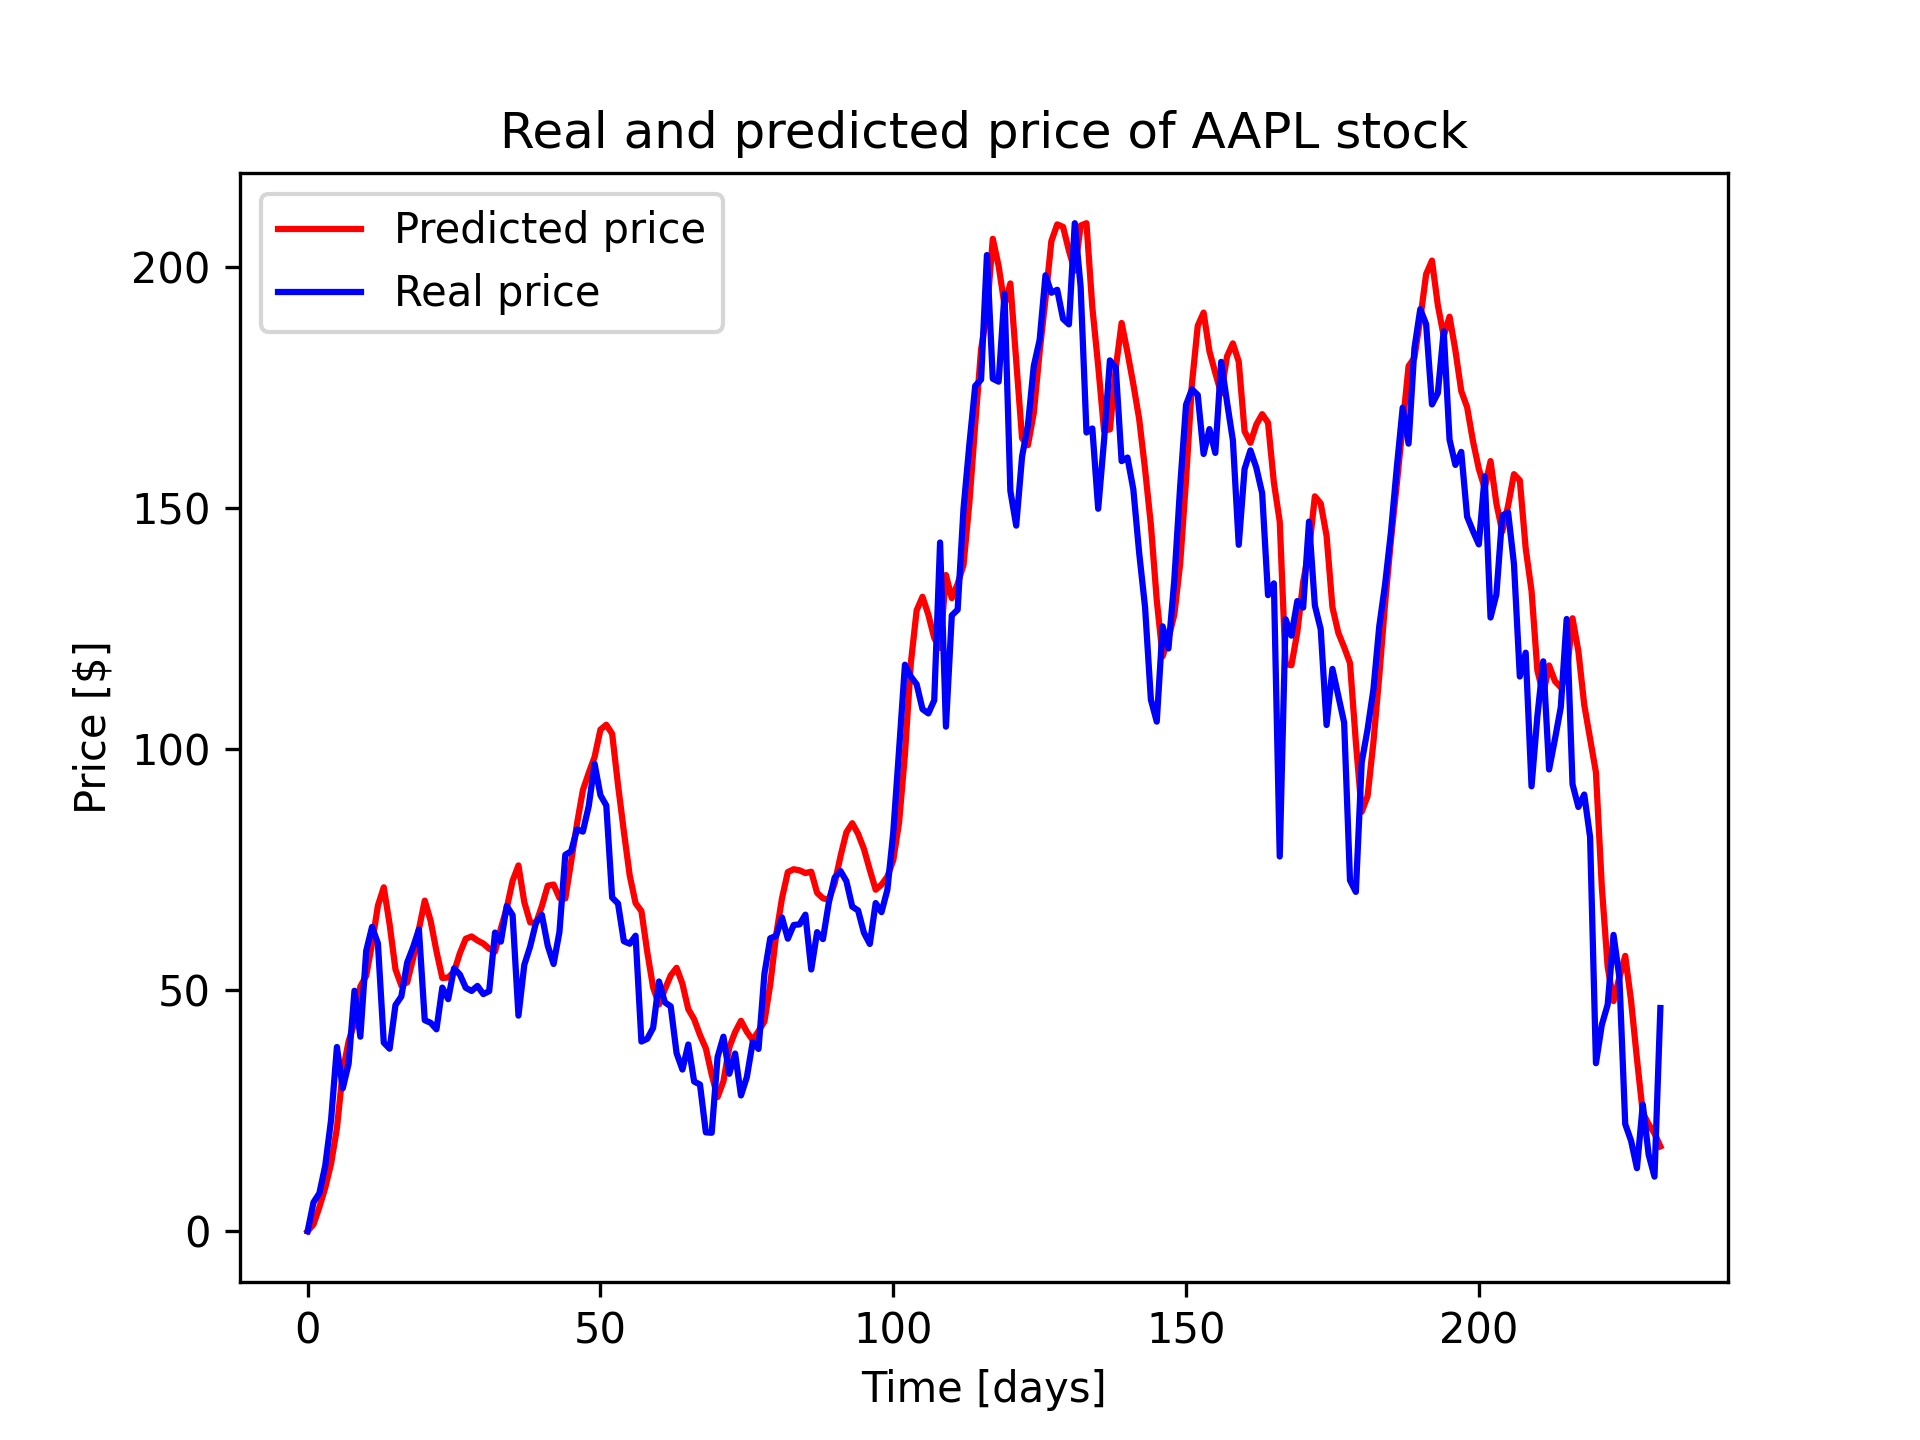
\includegraphics[width=0.5\textwidth]{./graf/model3/AAPL.png}
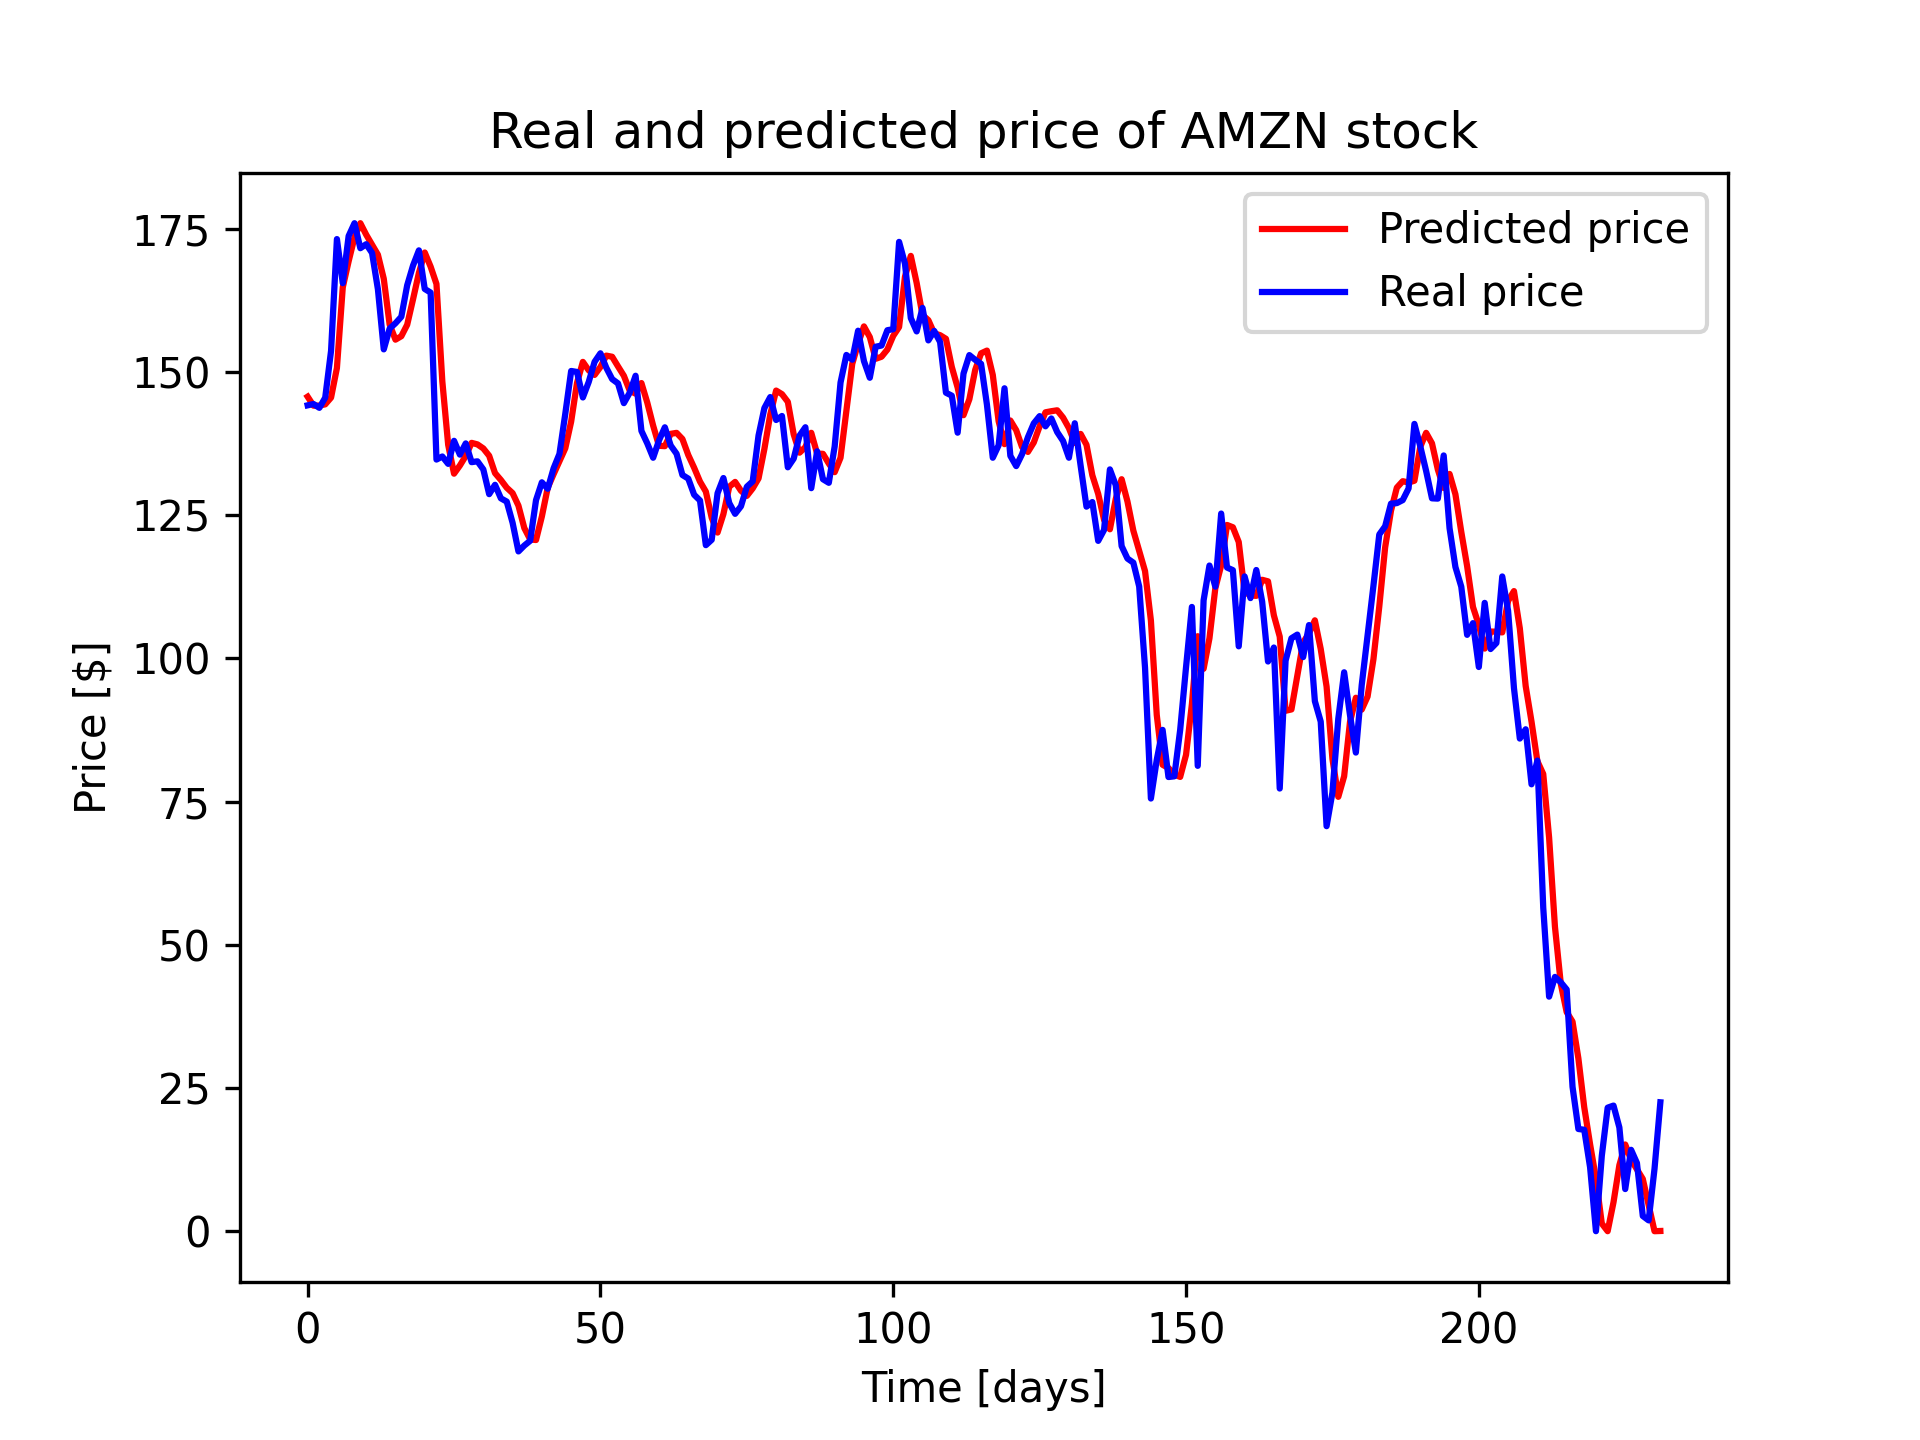
\includegraphics[width=0.5\textwidth]{./graf/model3/AMZN.png}
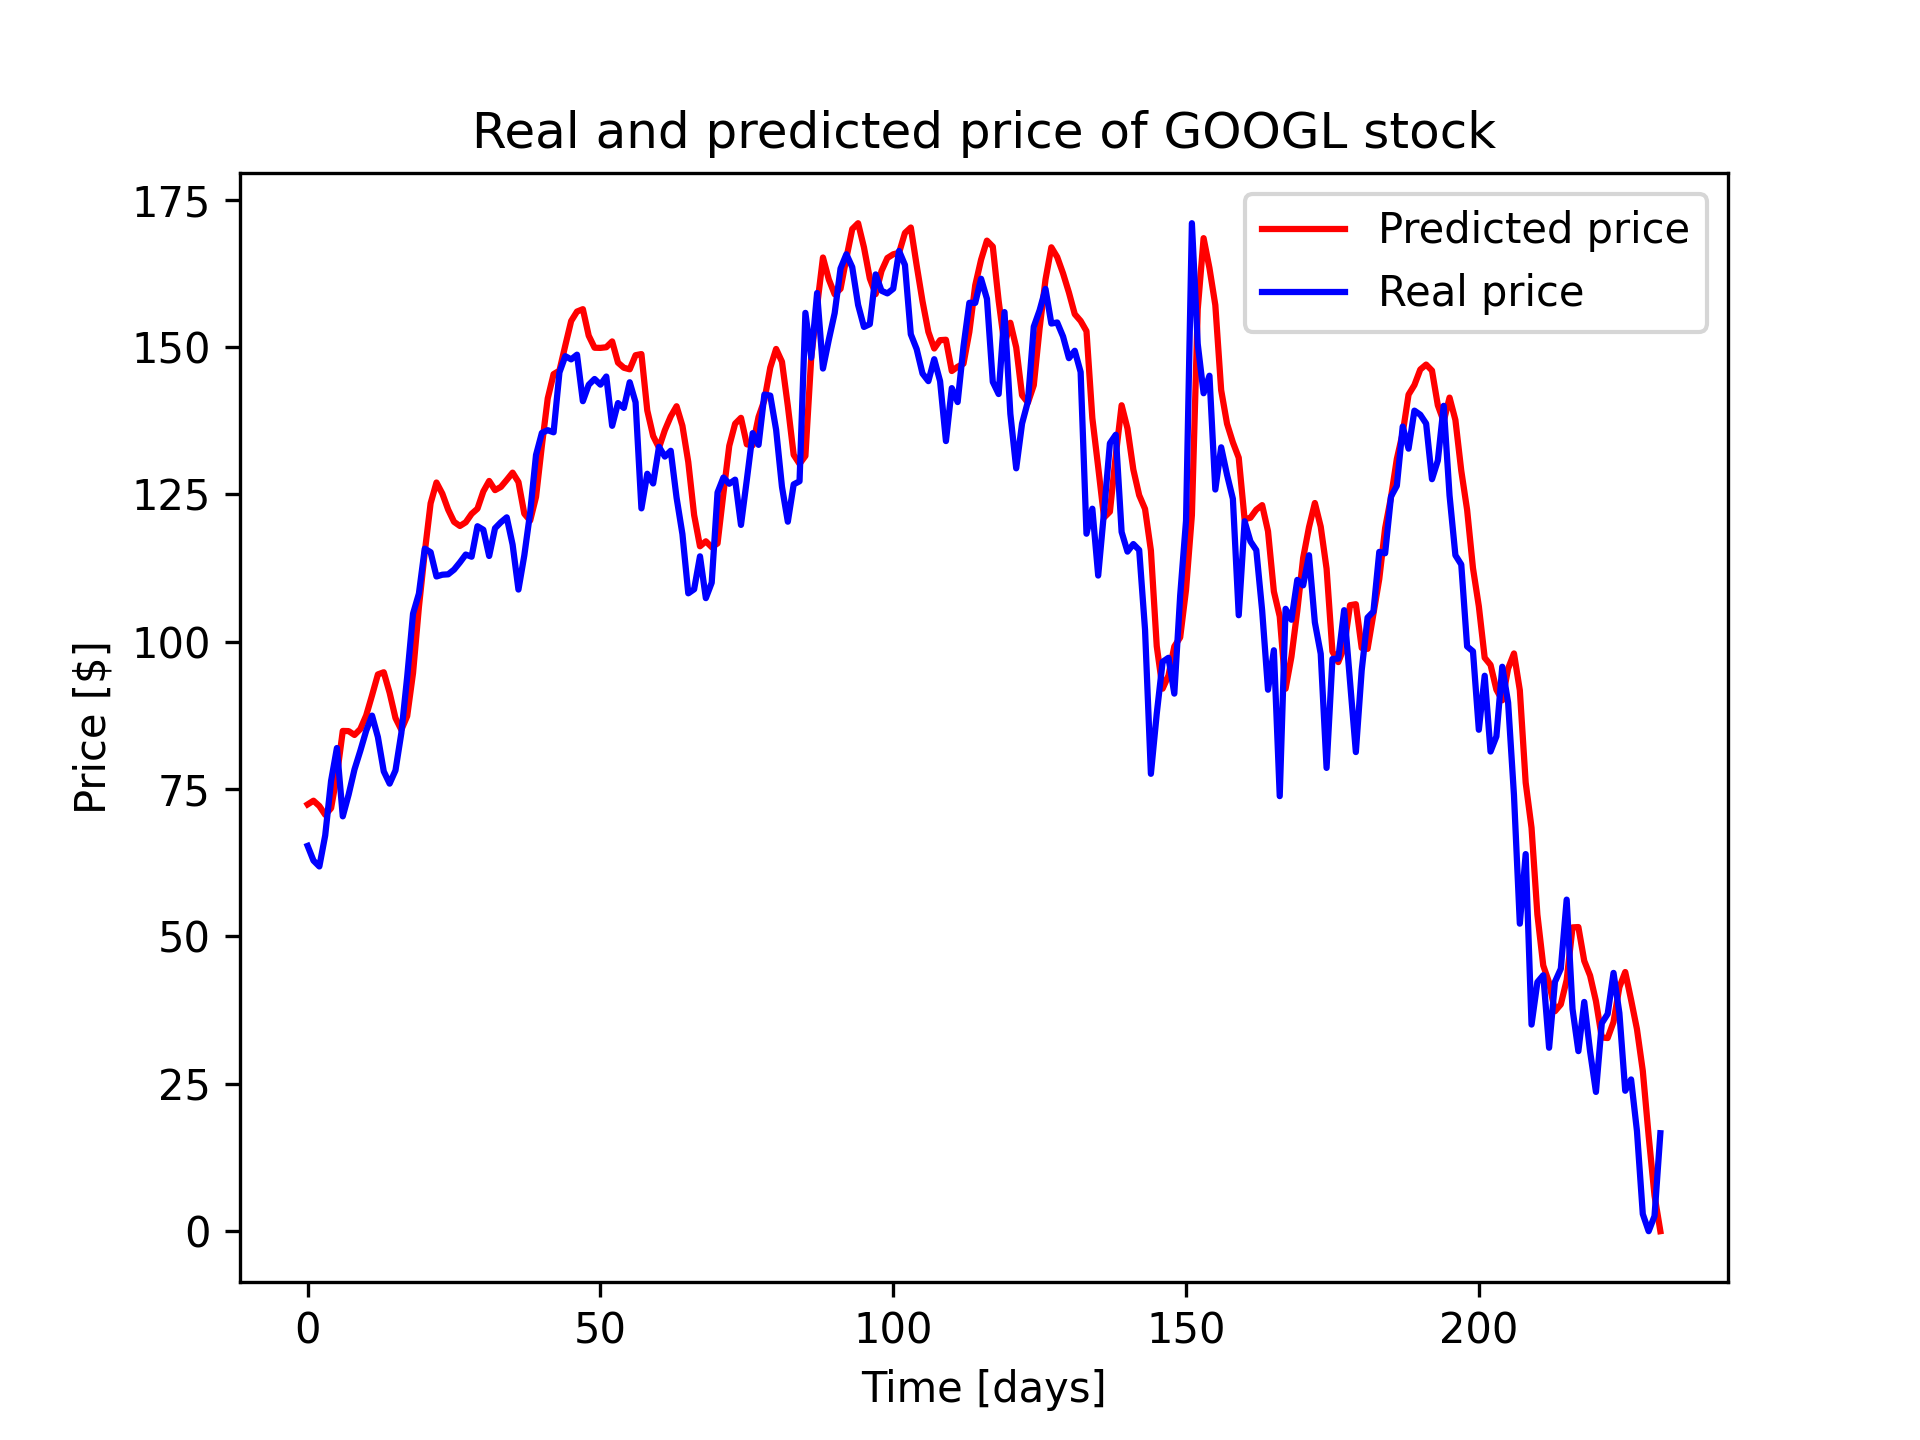
\includegraphics[width=0.5\textwidth]{./graf/model3/GOOGL.png}
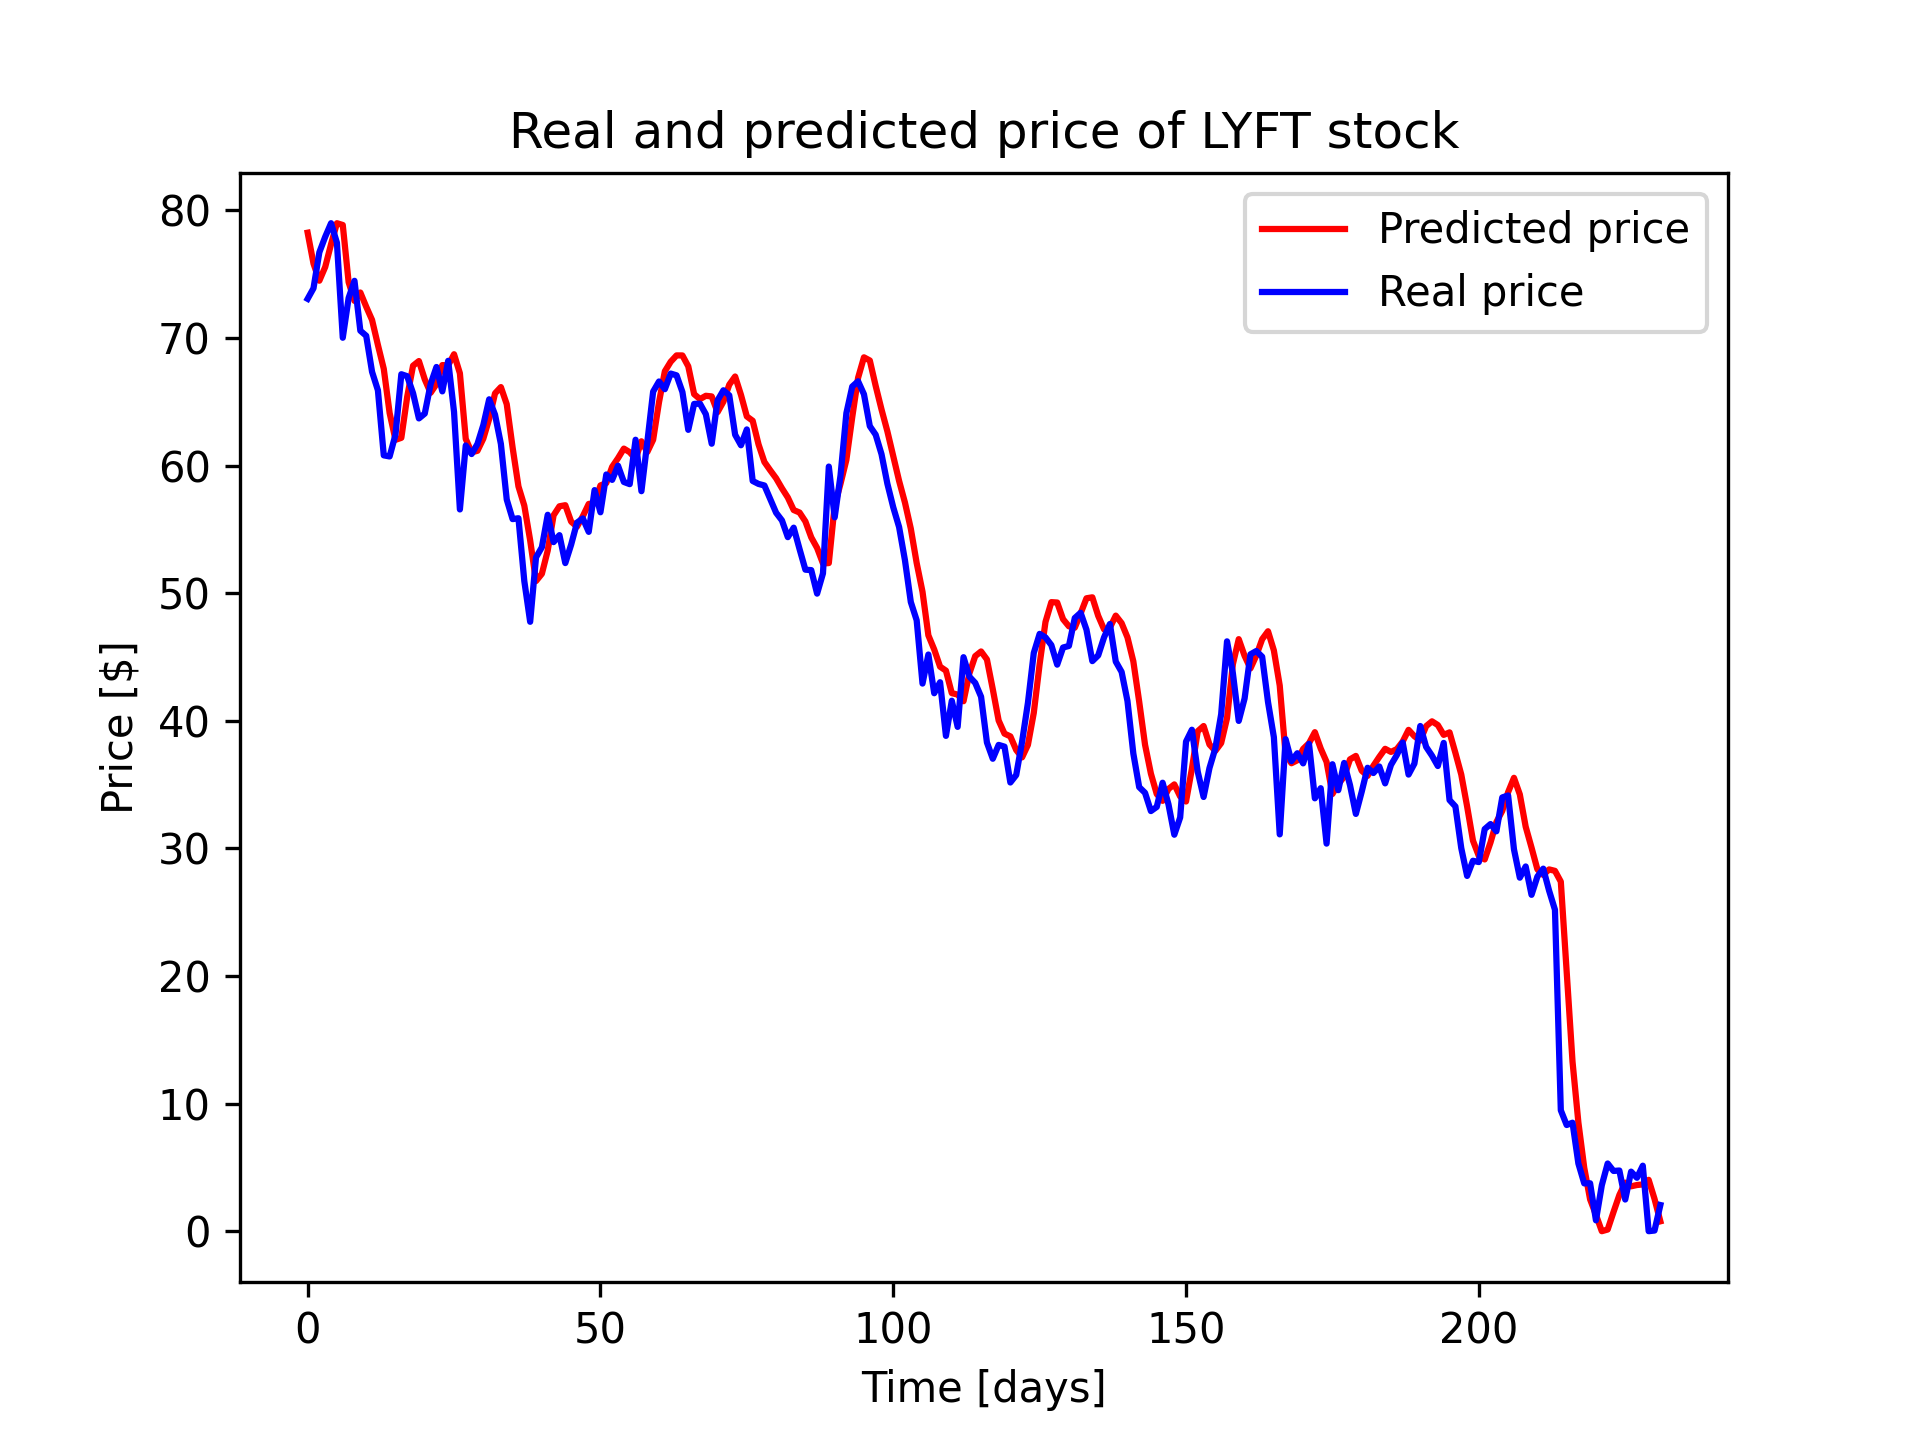
\includegraphics[width=0.5\textwidth]{./graf/model3/LYFT.png}
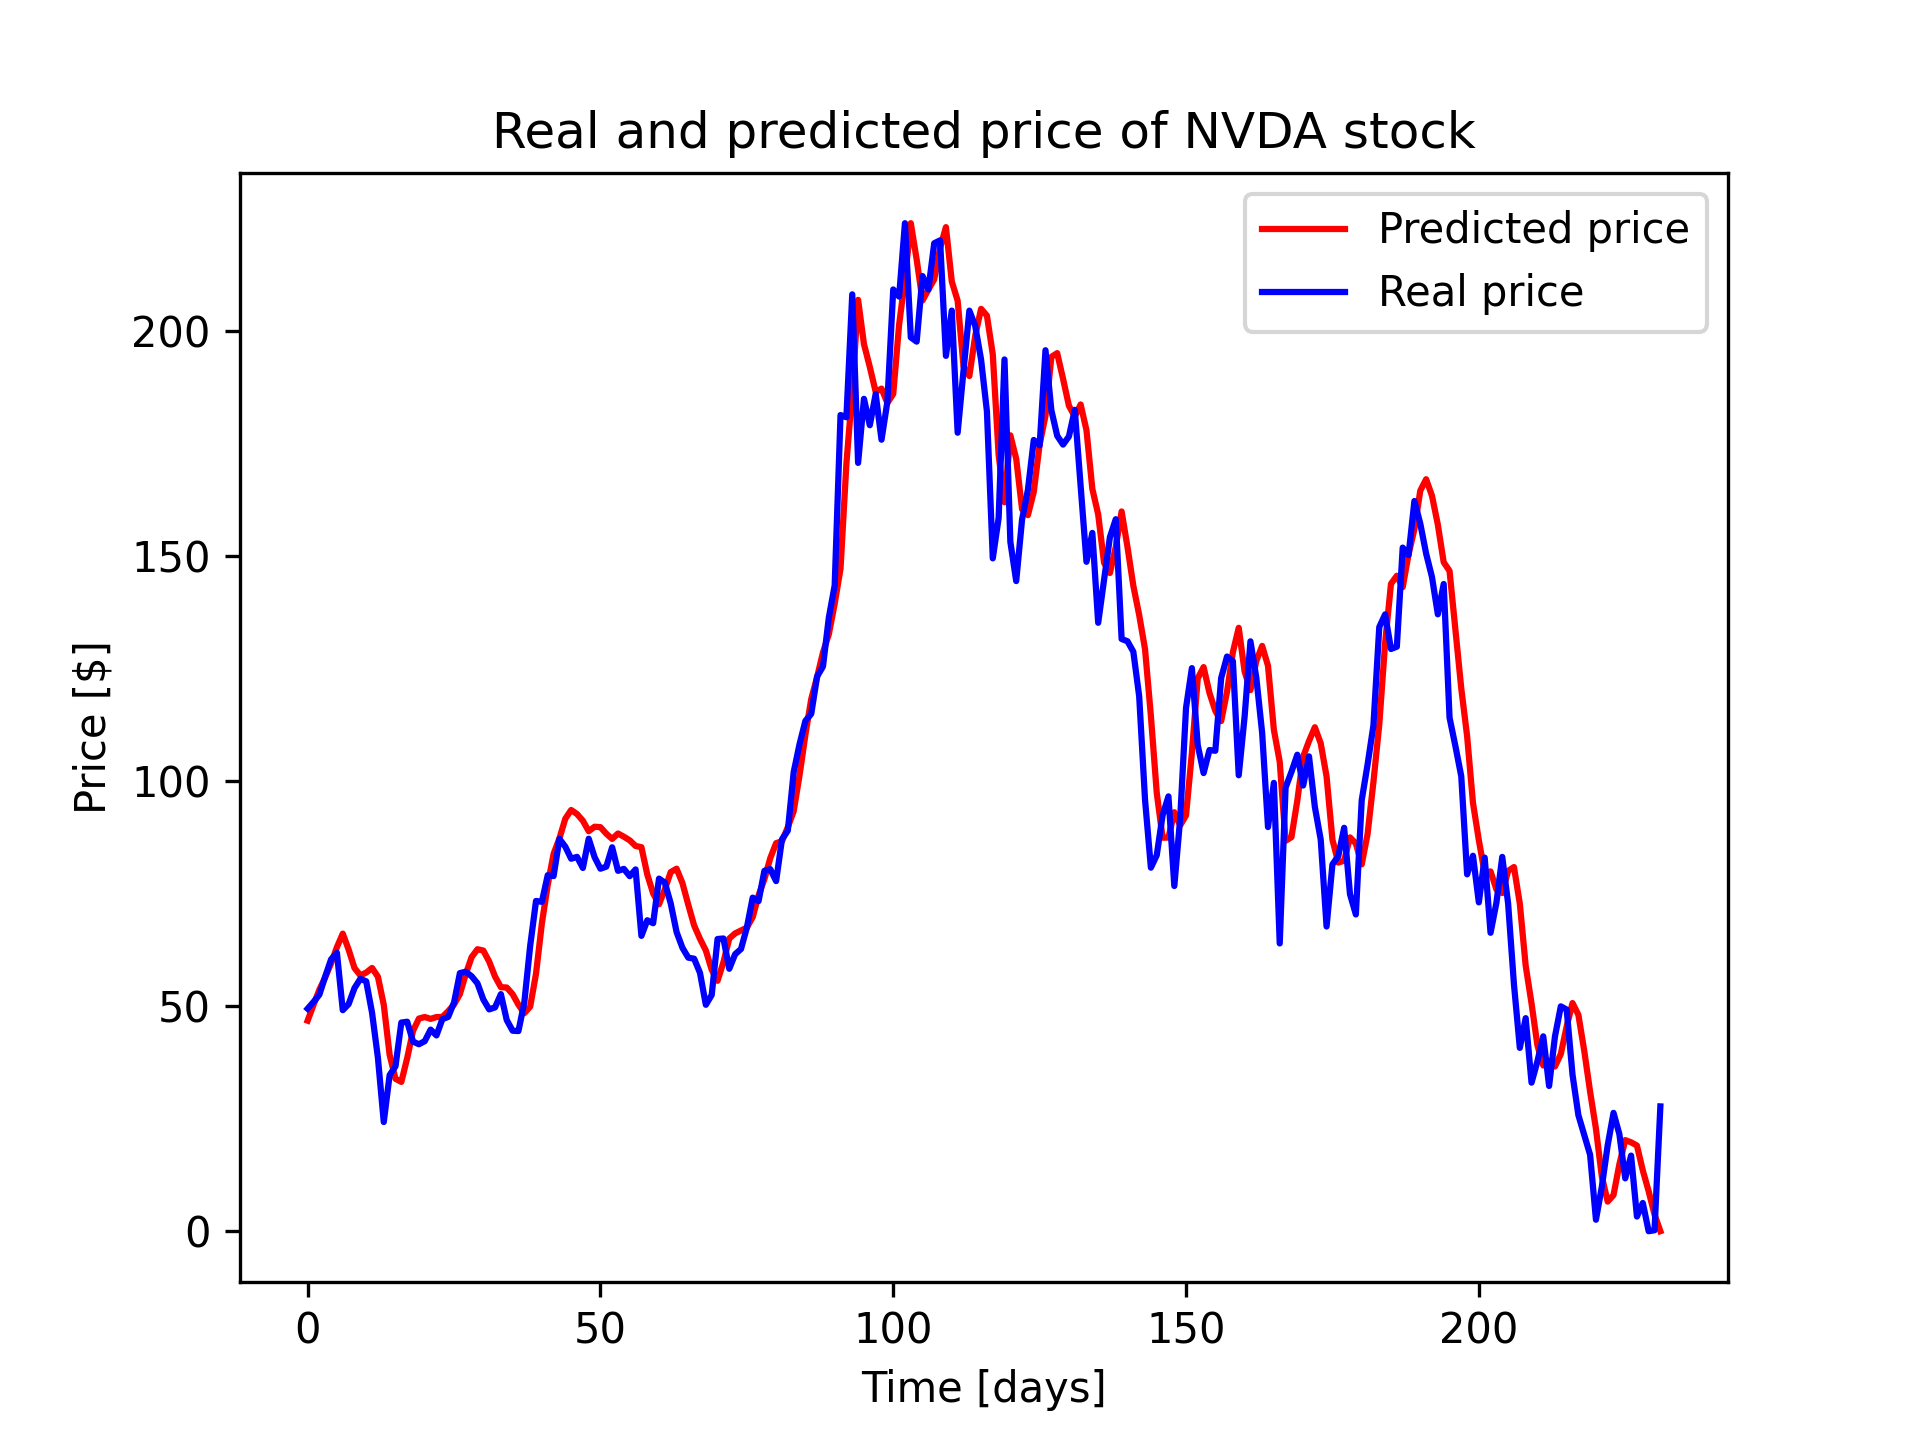
\includegraphics[width=0.5\textwidth]{./graf/model3/NVDA.png}
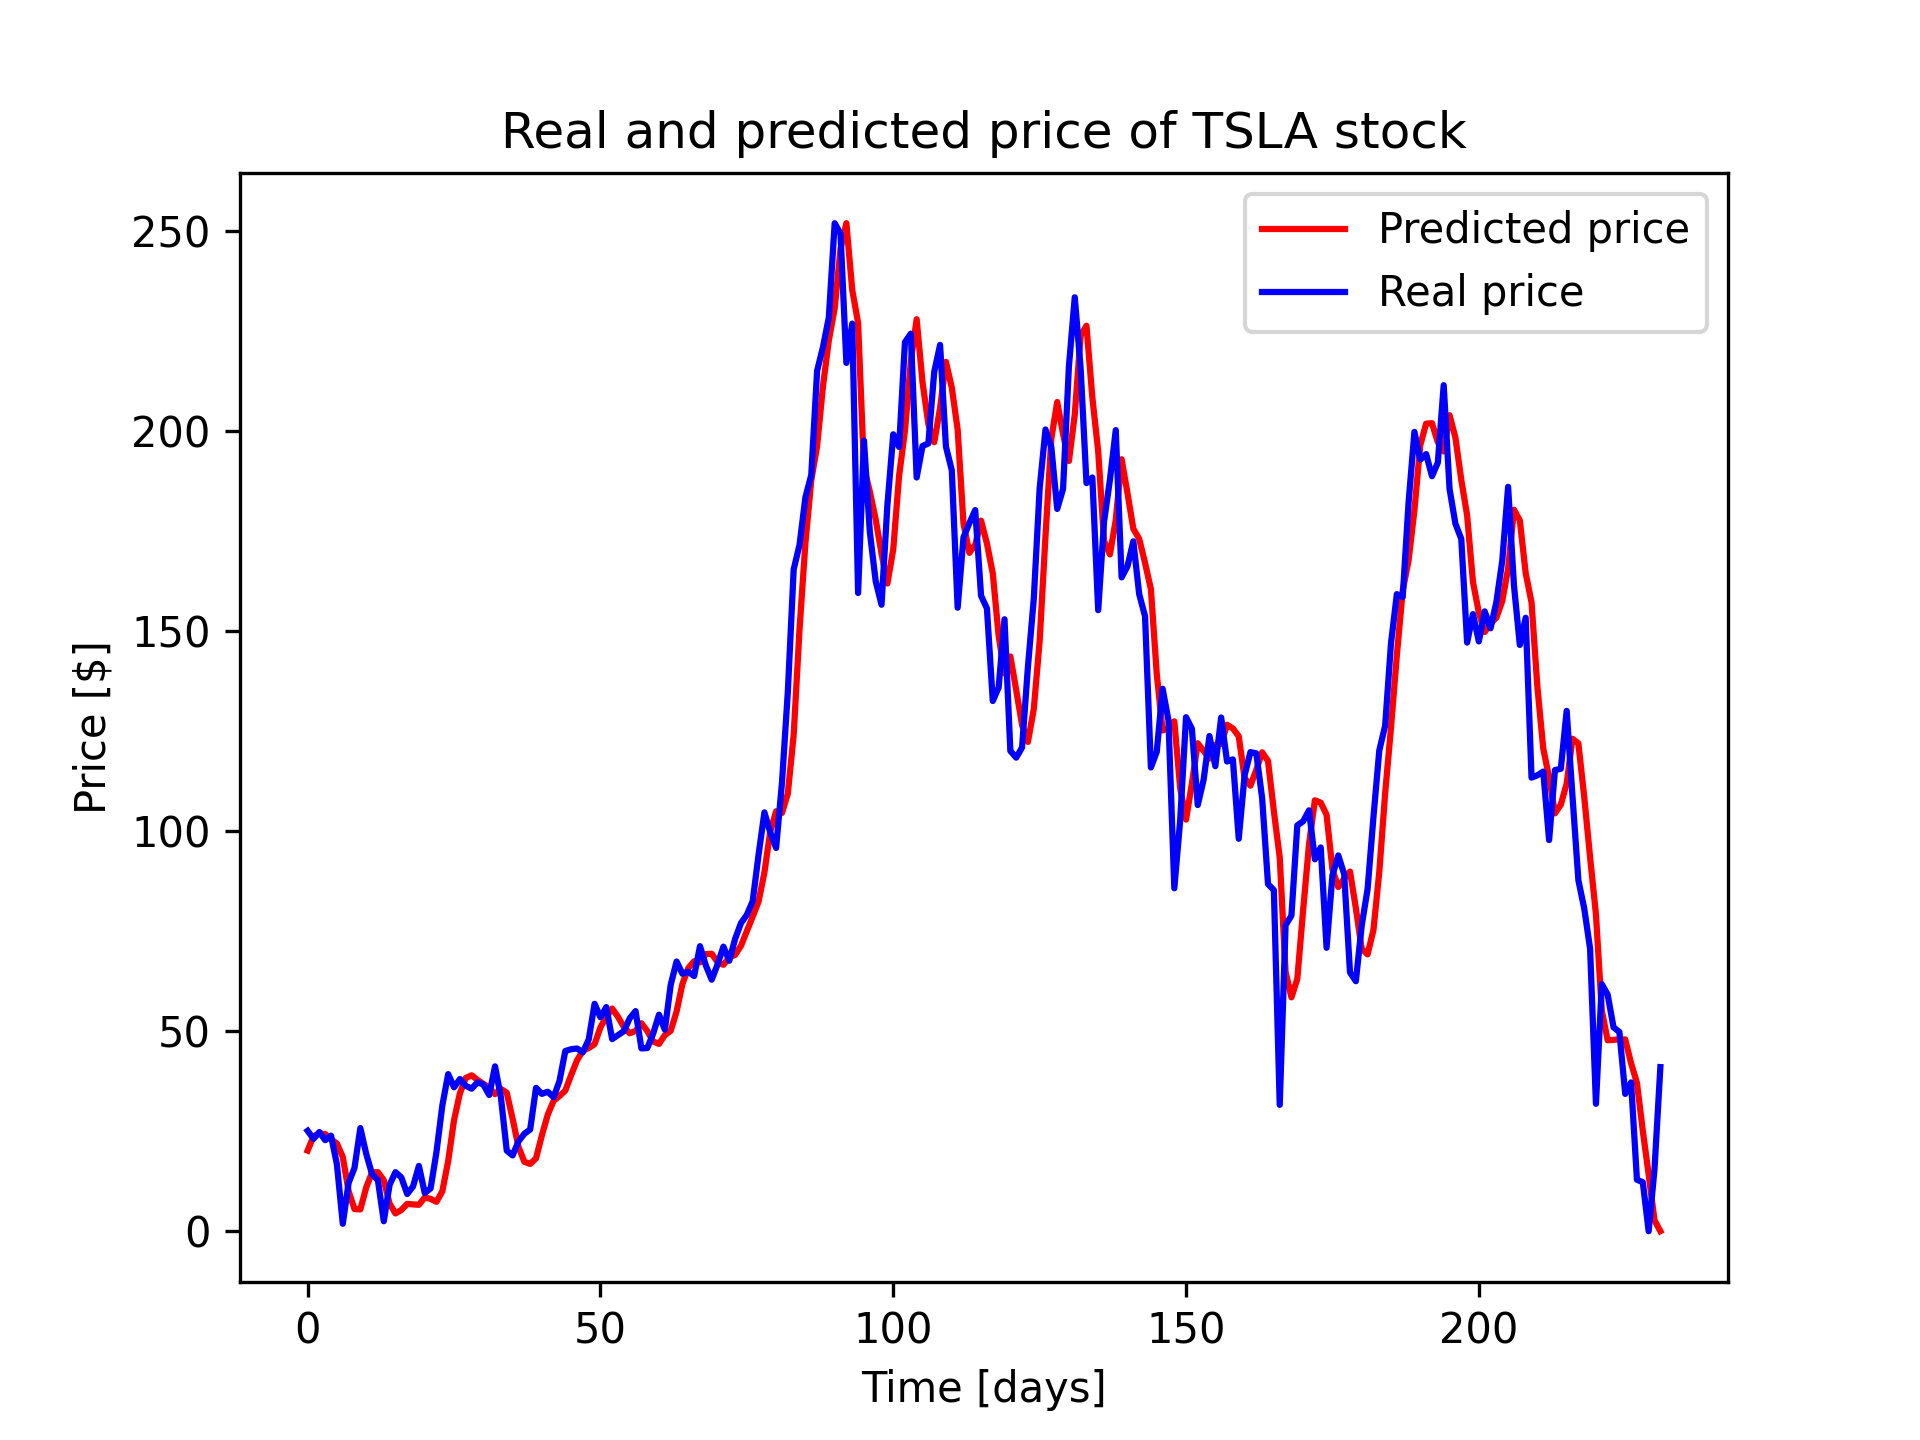
\includegraphics[width=0.5\textwidth]{./graf/model3/TSLA.png}
\caption{Real and predicted prices of the third model.}
\label{fig:label}
\end{figure} 

\clearpage
\subsection{Model 4}

Model4 - chunkSize: 50, time interval: 1 year, epochs: 5, trained on AAPL\par\bigskip
Analyzing model 4 in terms of the convergence of the predicted price to the real price, it can be seen that in places where the amplitude swings sharply, there are discrepancies in the course of
both lines relative to each other. In the AMZN.png and LYFT.png charts, the red line runs slightly
ahead of the real price line and is slightly above it. In the remaining charts, there is a tendency for
both lines to intersect in several areas. The red line shows short-term price fluctuations in minor
detail, showing only the general direction of the downward or upward trend.
\par\bigskip
loss: 0.009654750116169453\par
RMSE for AAPL equals 8.90622068107363\par
RMSE for AMZN equals 7.511405804149795\par
RMSE for GOOGL equals 5.3093154596807794\par
RMSE for LYFT equals 1.9880919617118793\par
RMSE for NVDA equals 6.67375019766115\par
RMSE for TSLA equals 0.586036519909922\par


\begin{figure}
% \centering
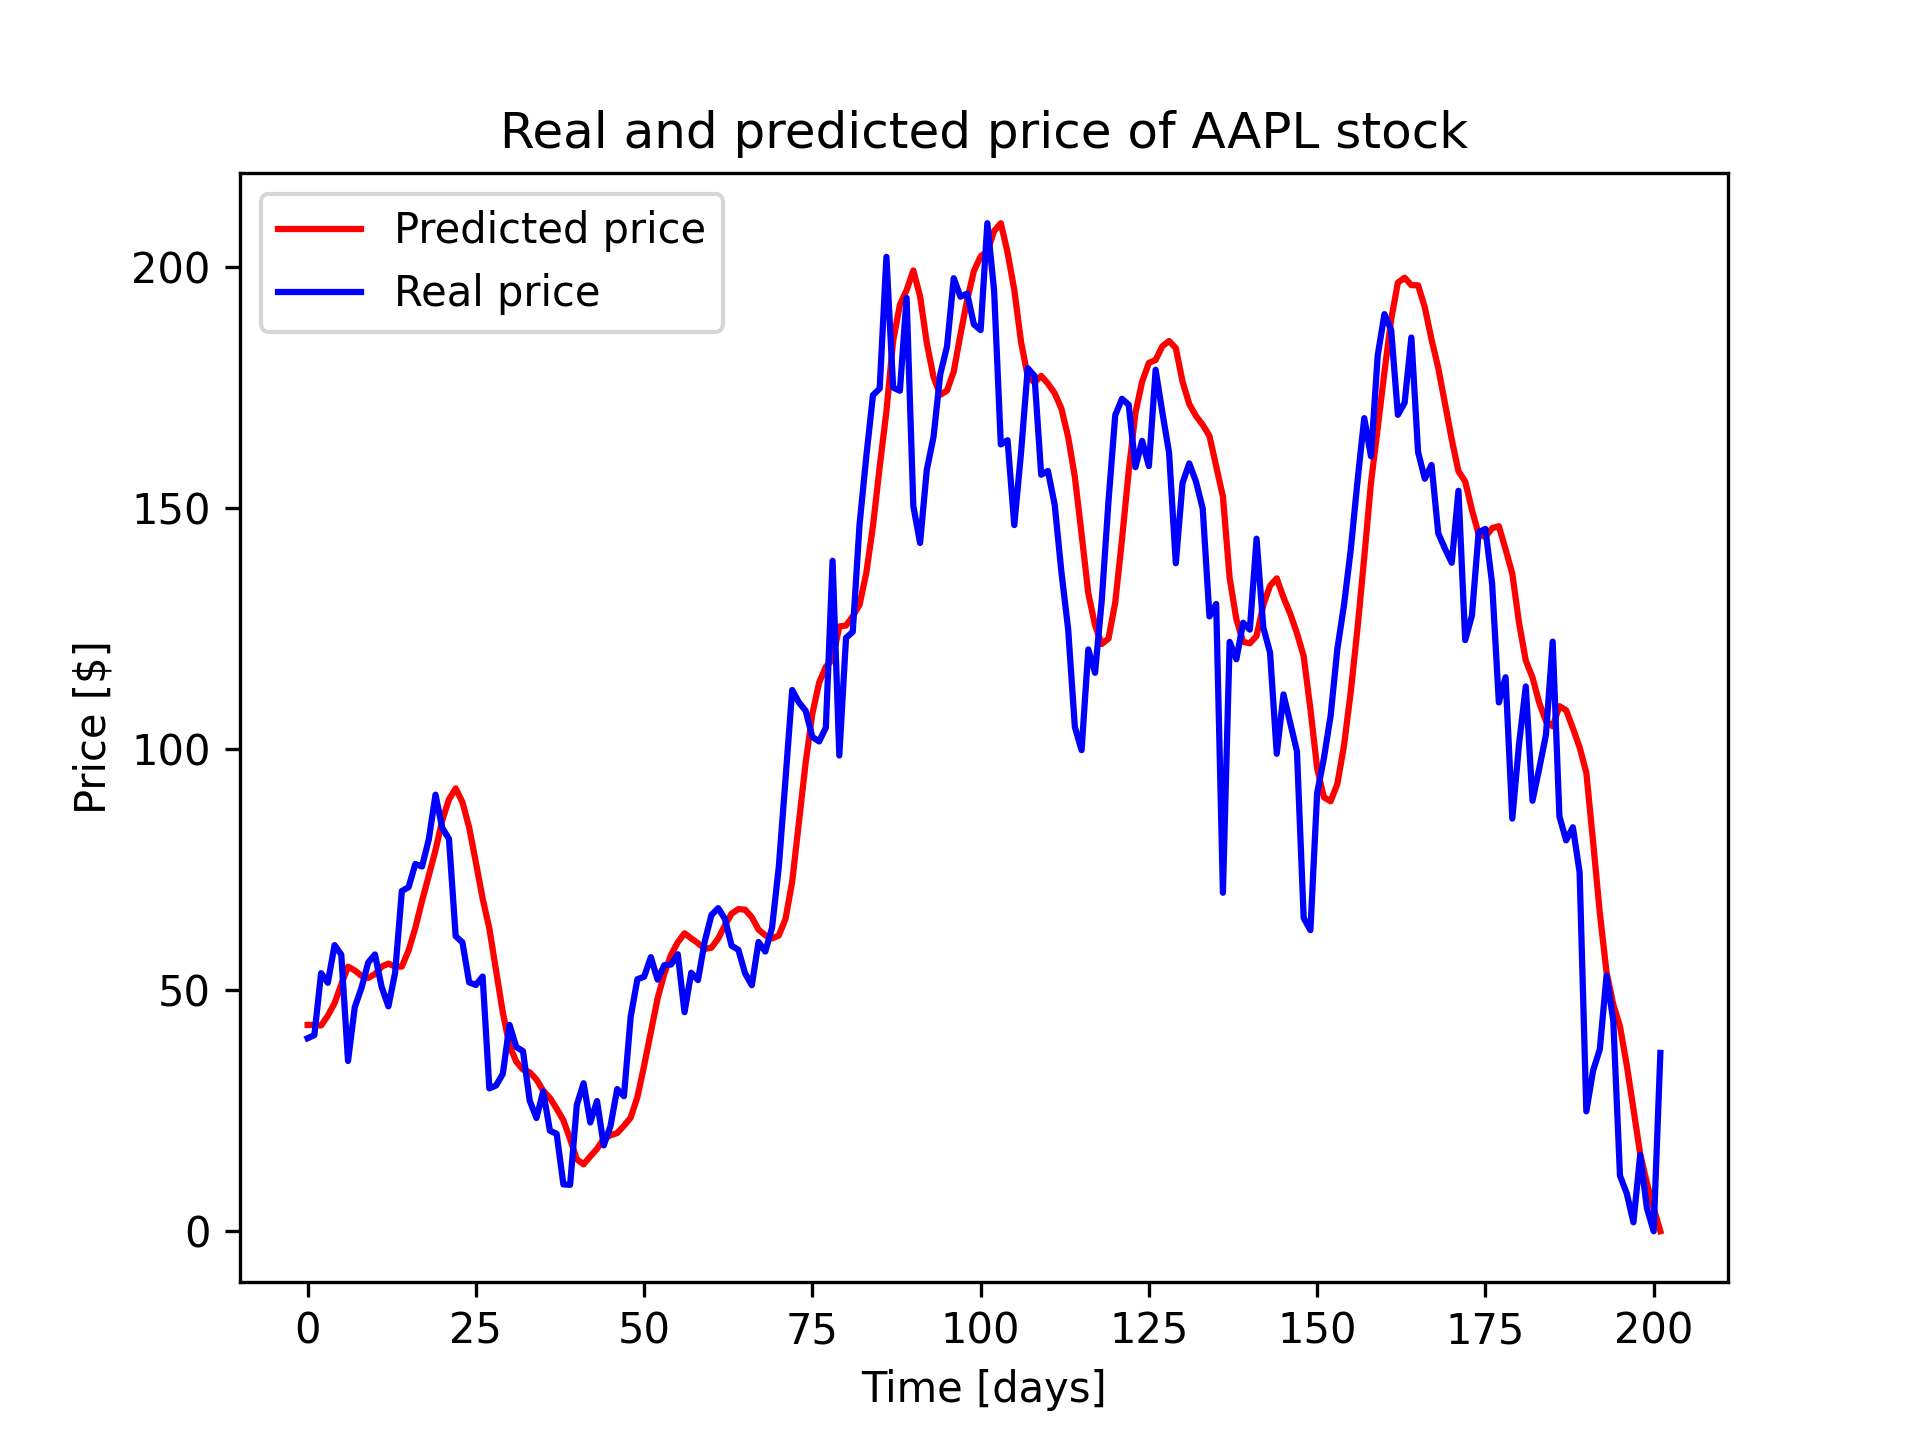
\includegraphics[width=0.5\textwidth]{./graf/model4/AAPL.png}
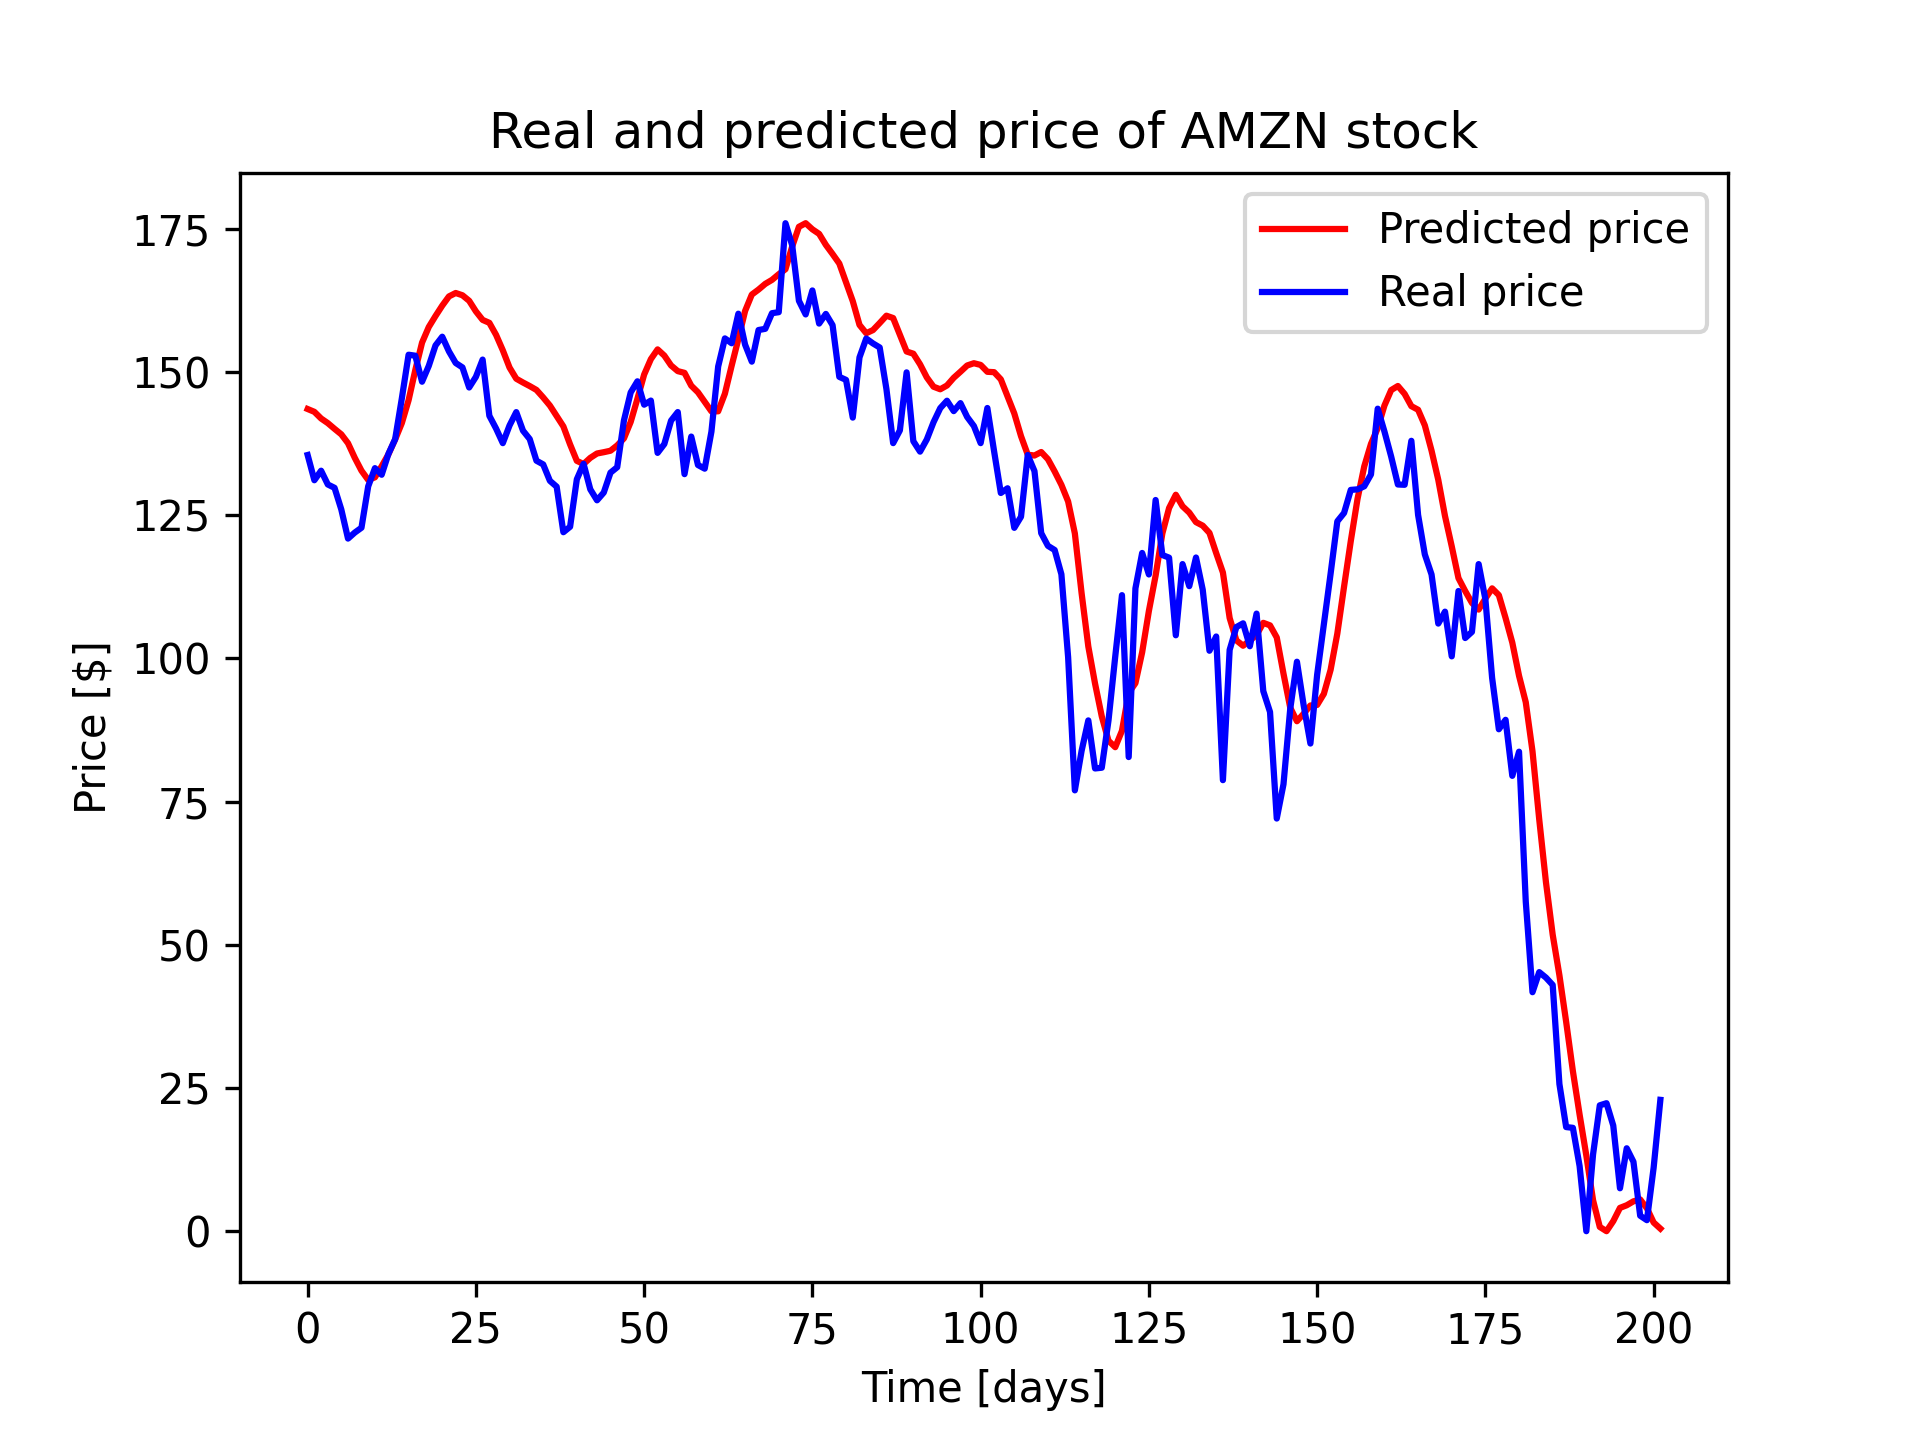
\includegraphics[width=0.5\textwidth]{./graf/model4/AMZN.png}
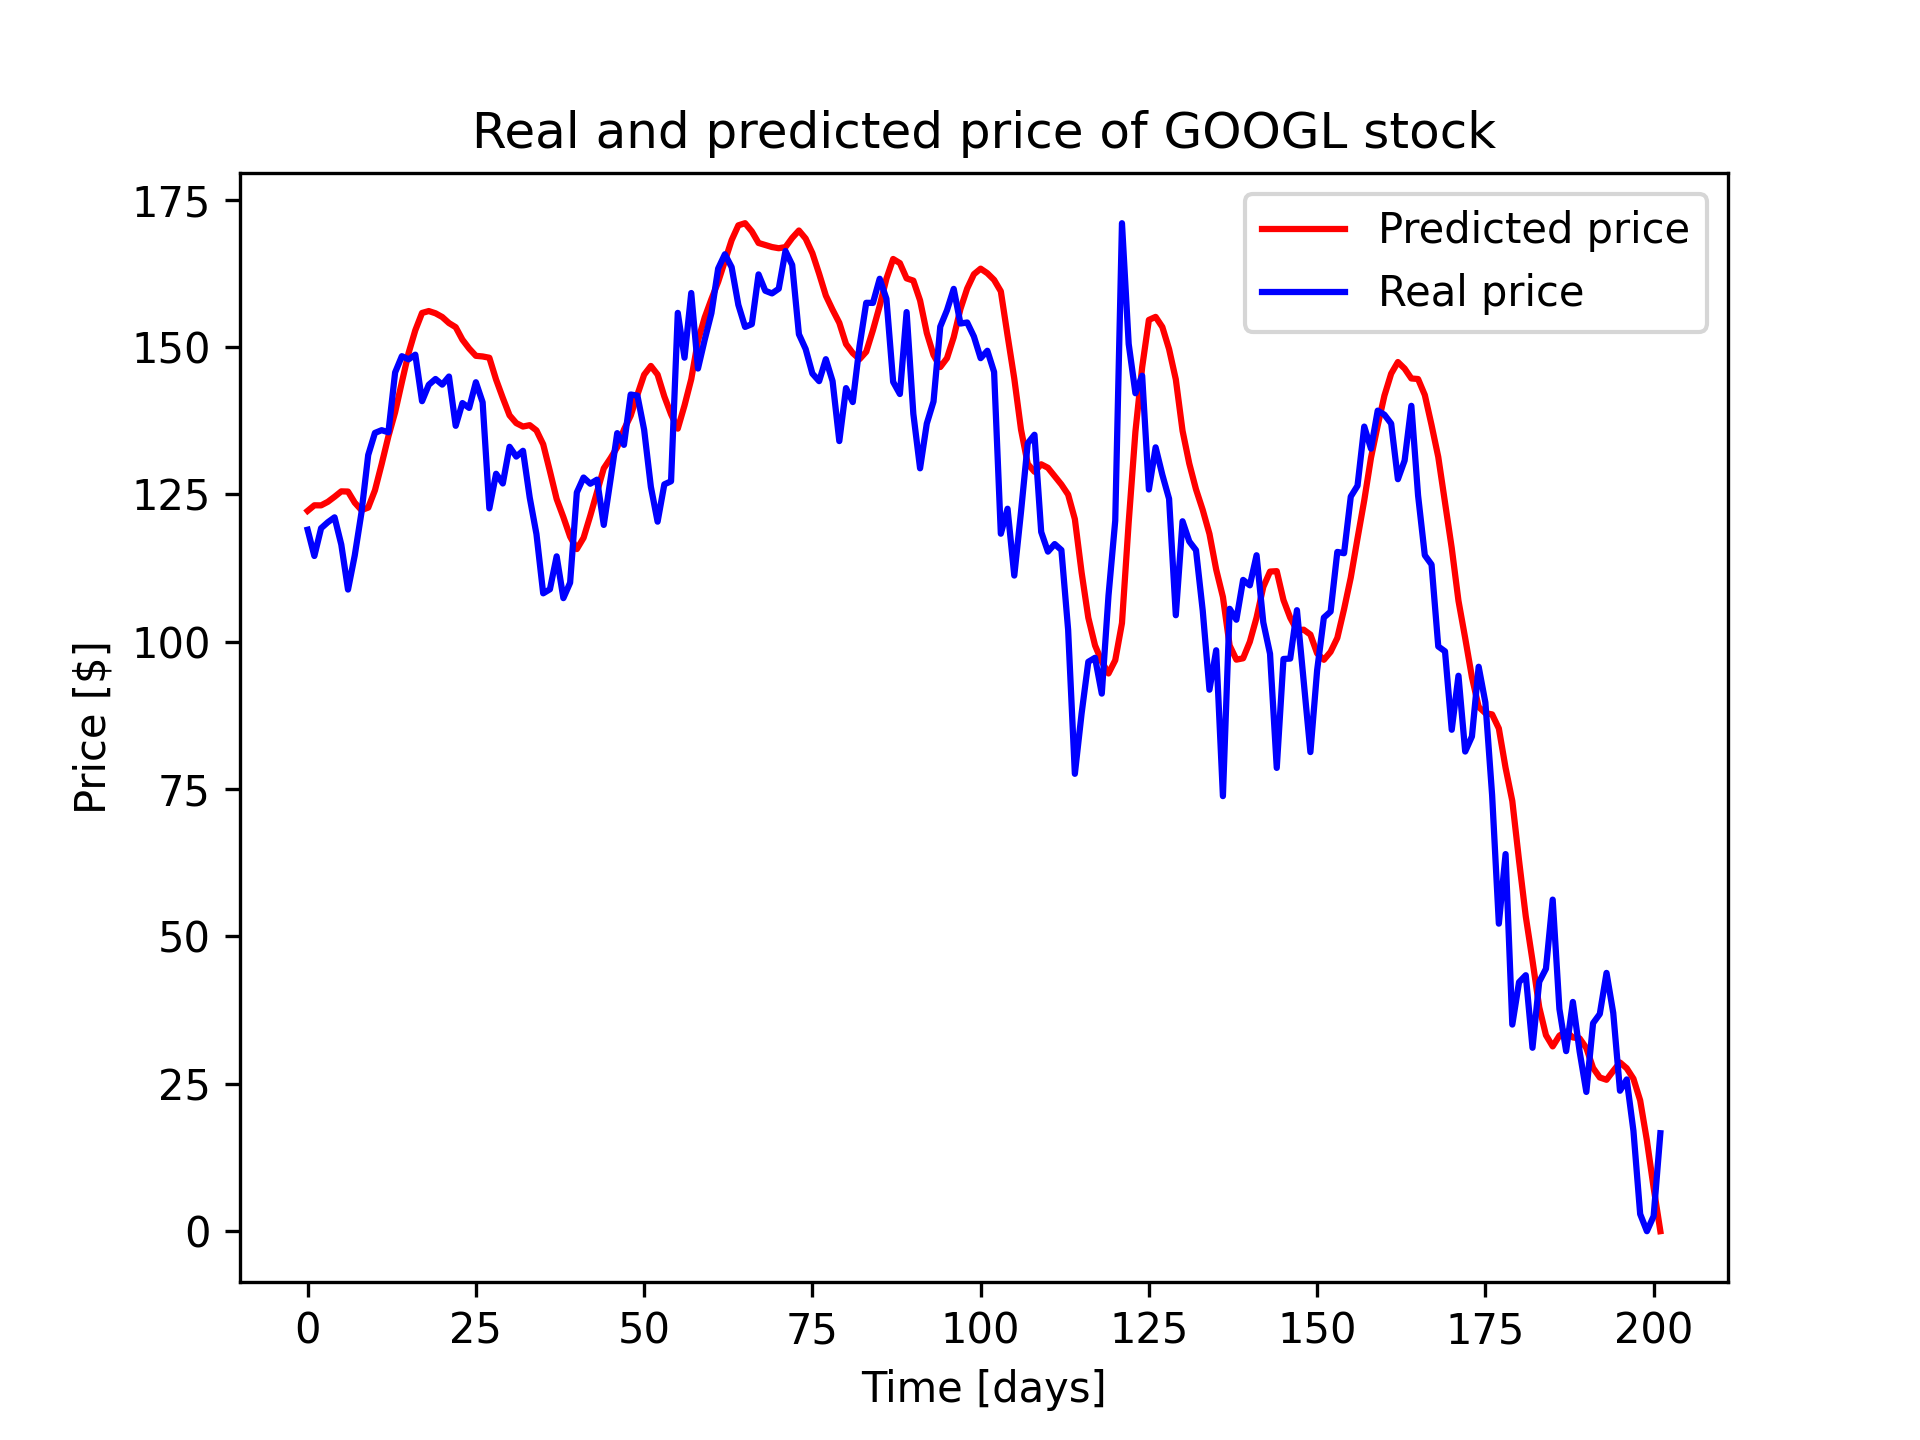
\includegraphics[width=0.5\textwidth]{./graf/model4/GOOGL.png}
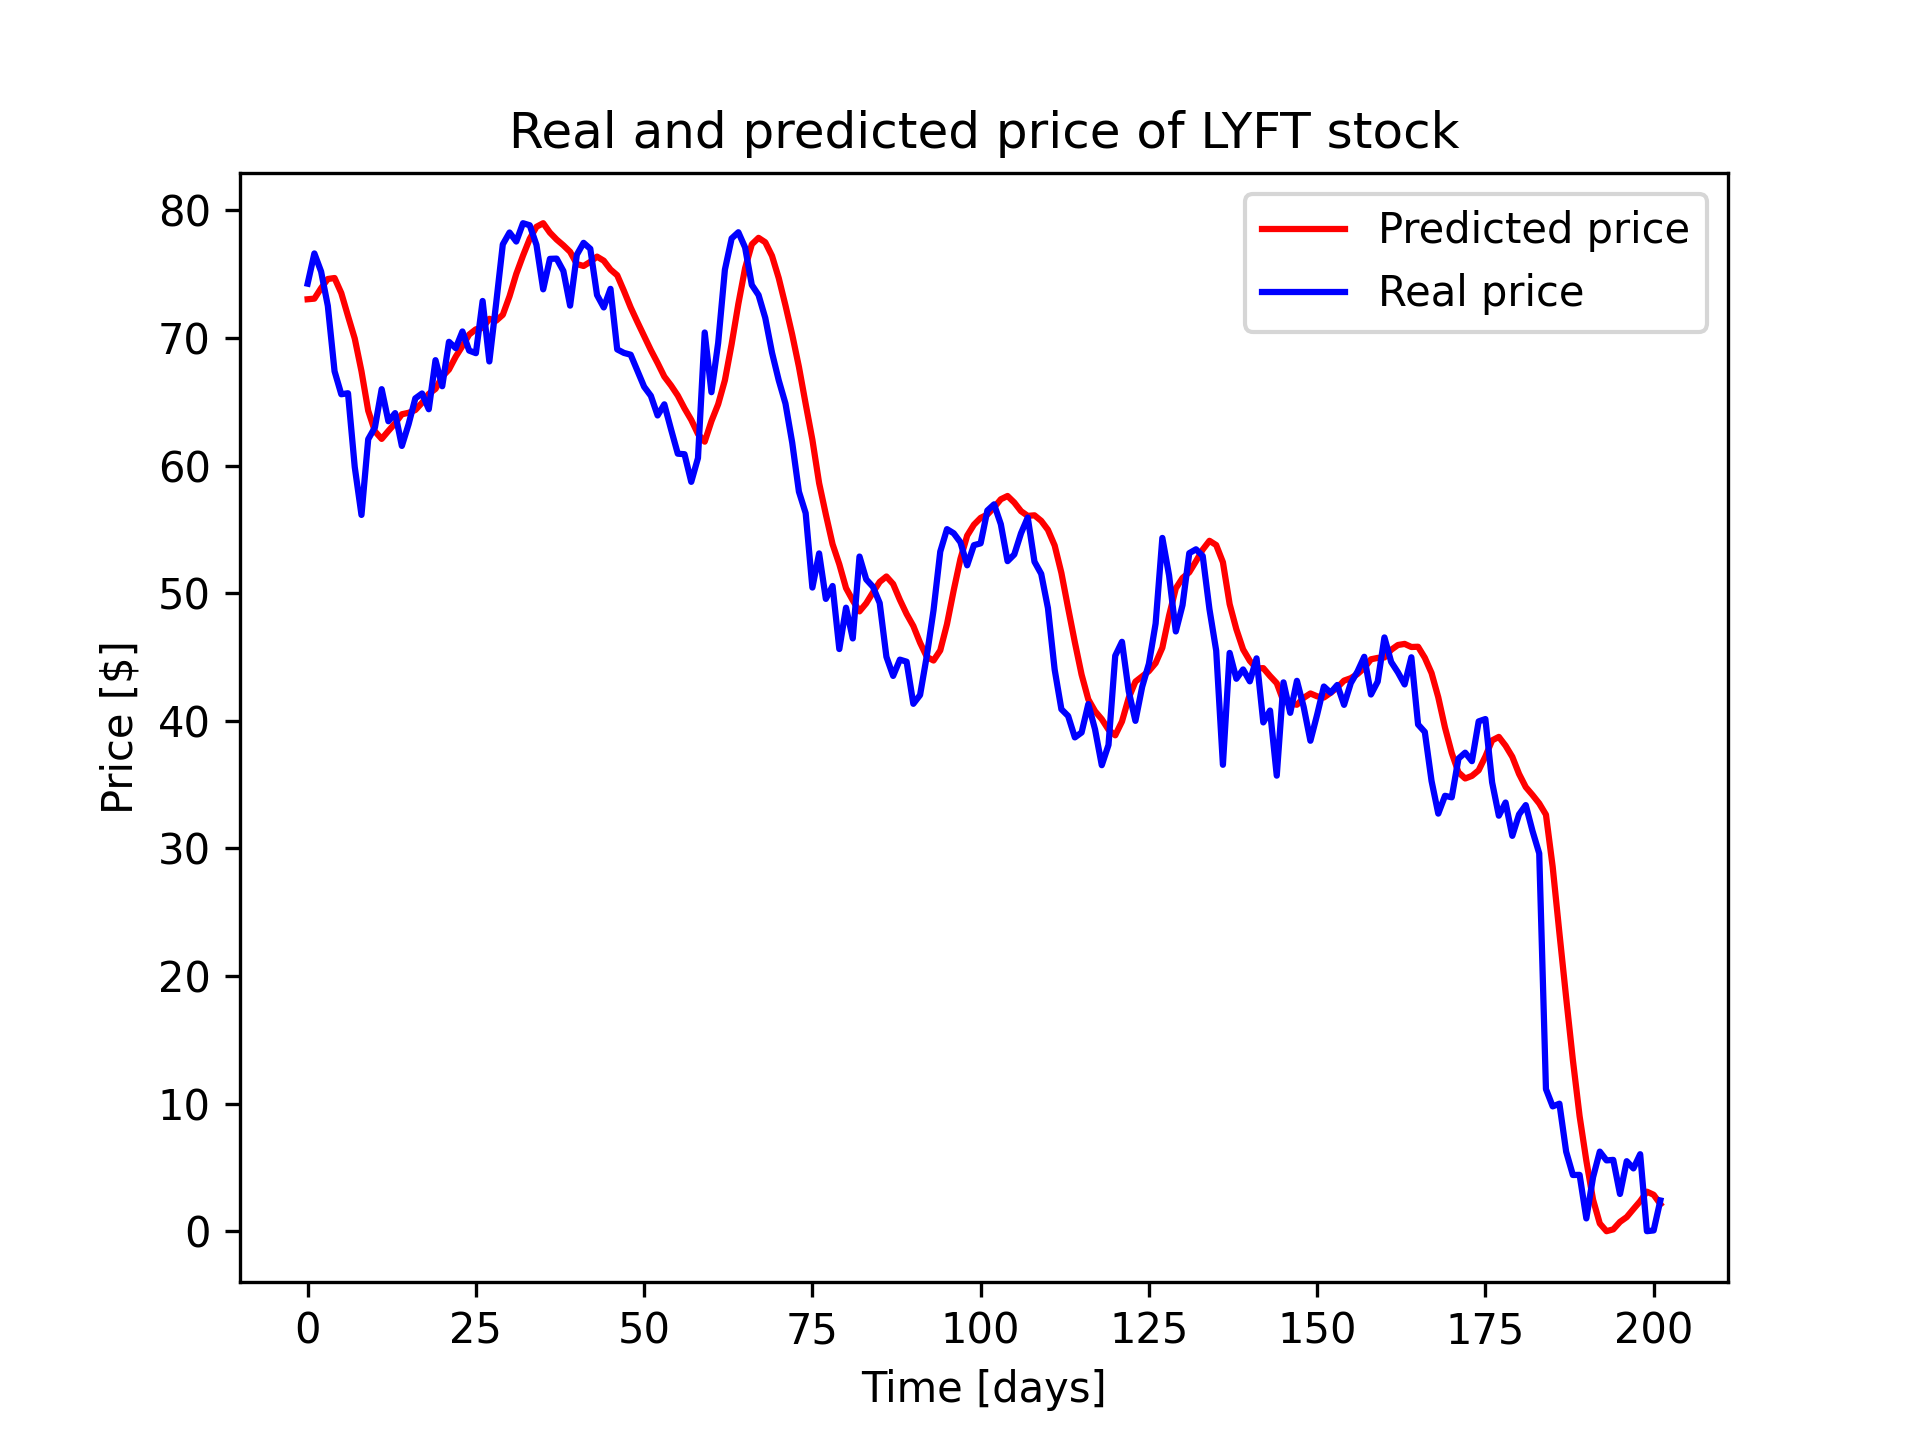
\includegraphics[width=0.5\textwidth]{./graf/model4/LYFT.png}
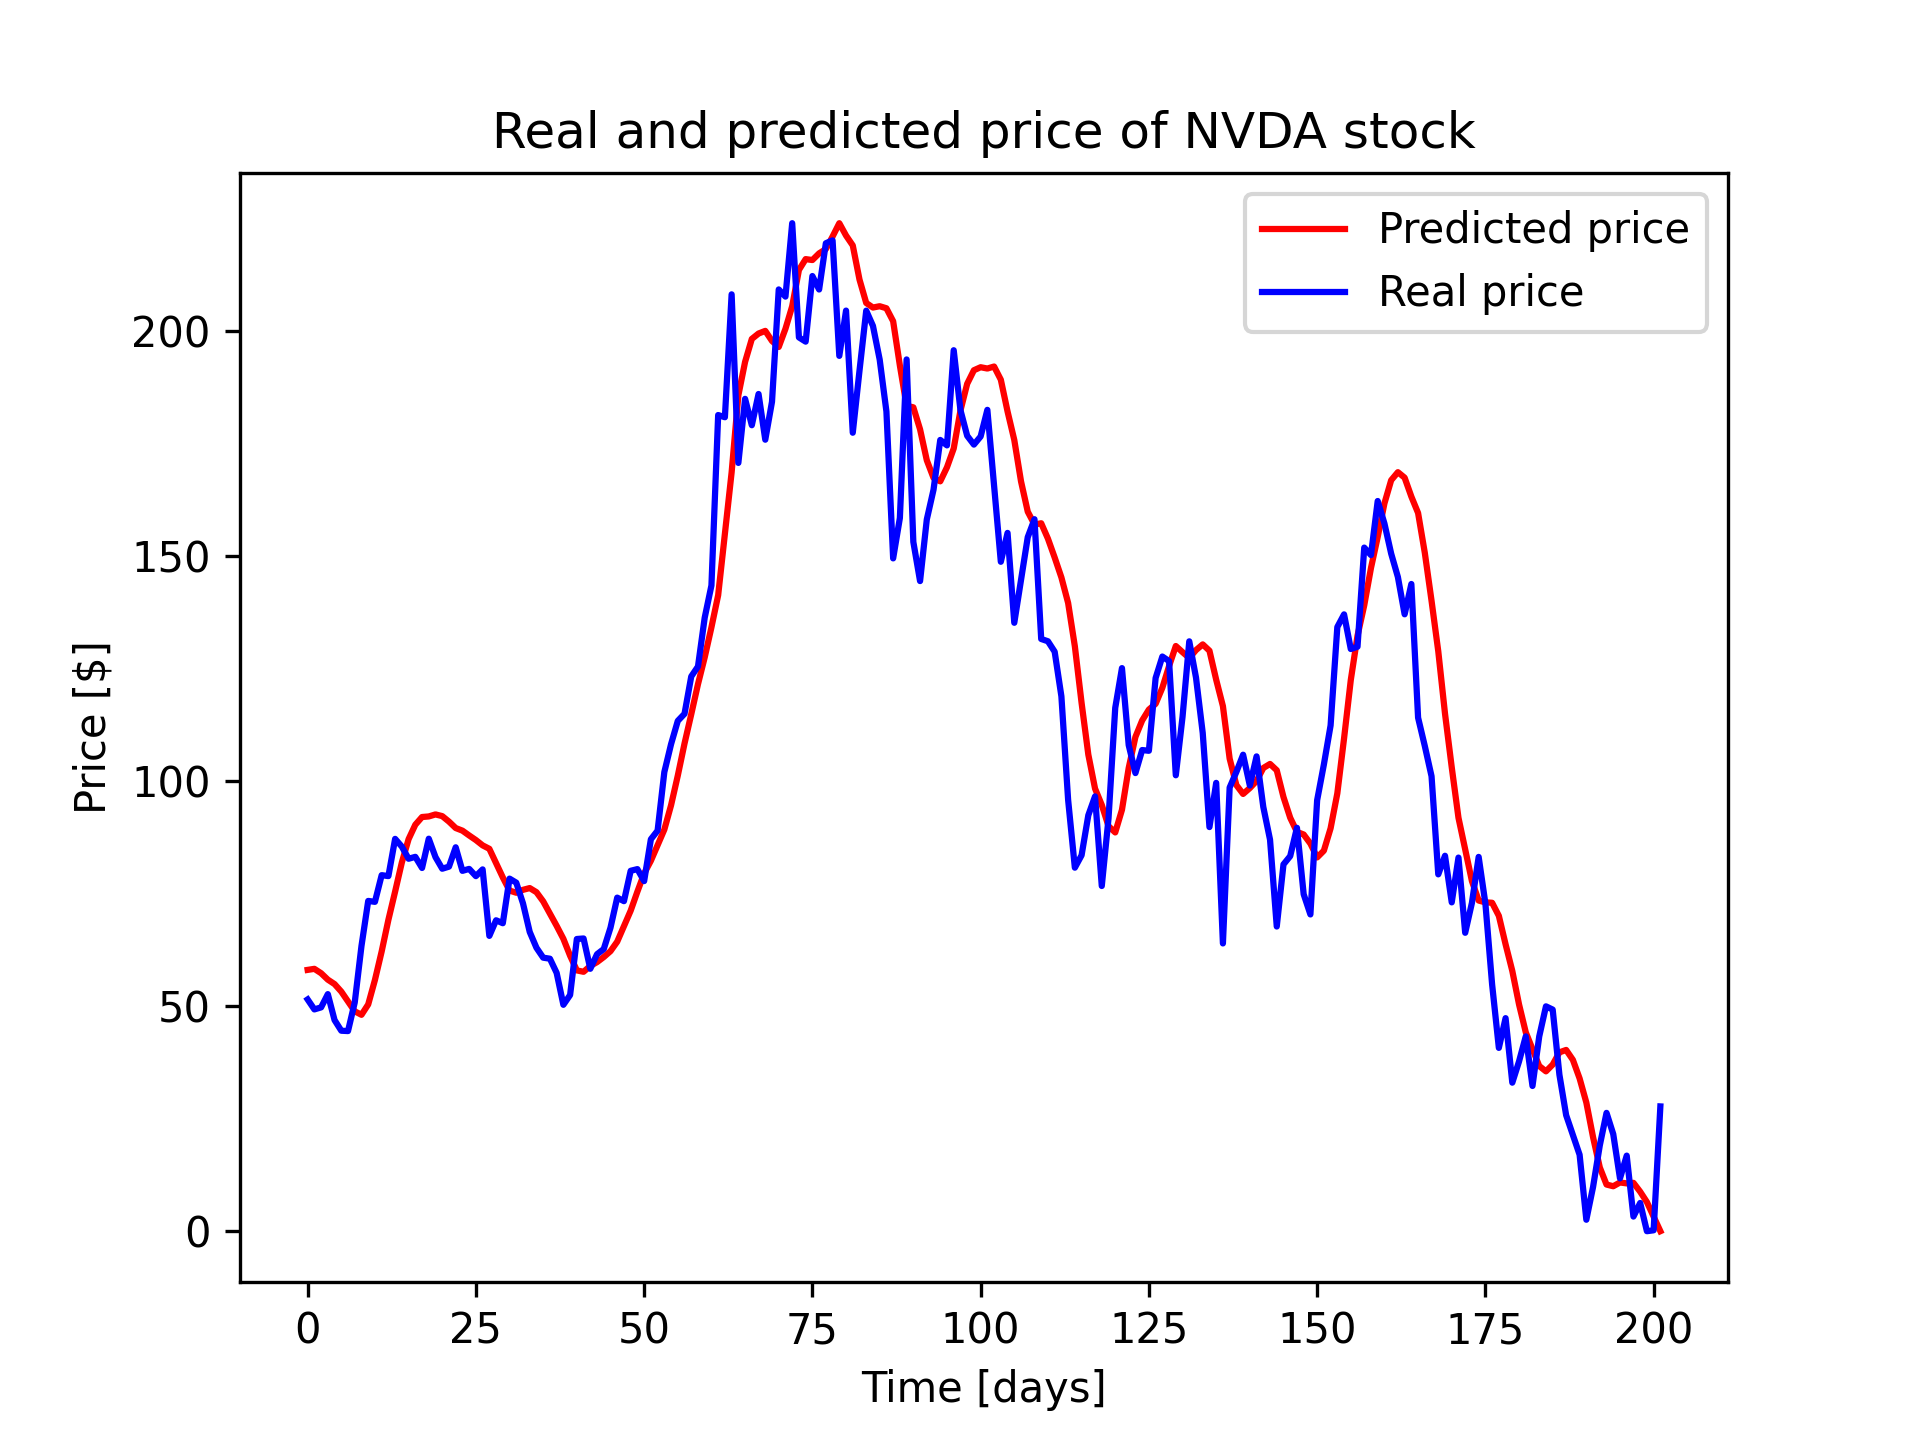
\includegraphics[width=0.5\textwidth]{./graf/model4/NVDA.png}
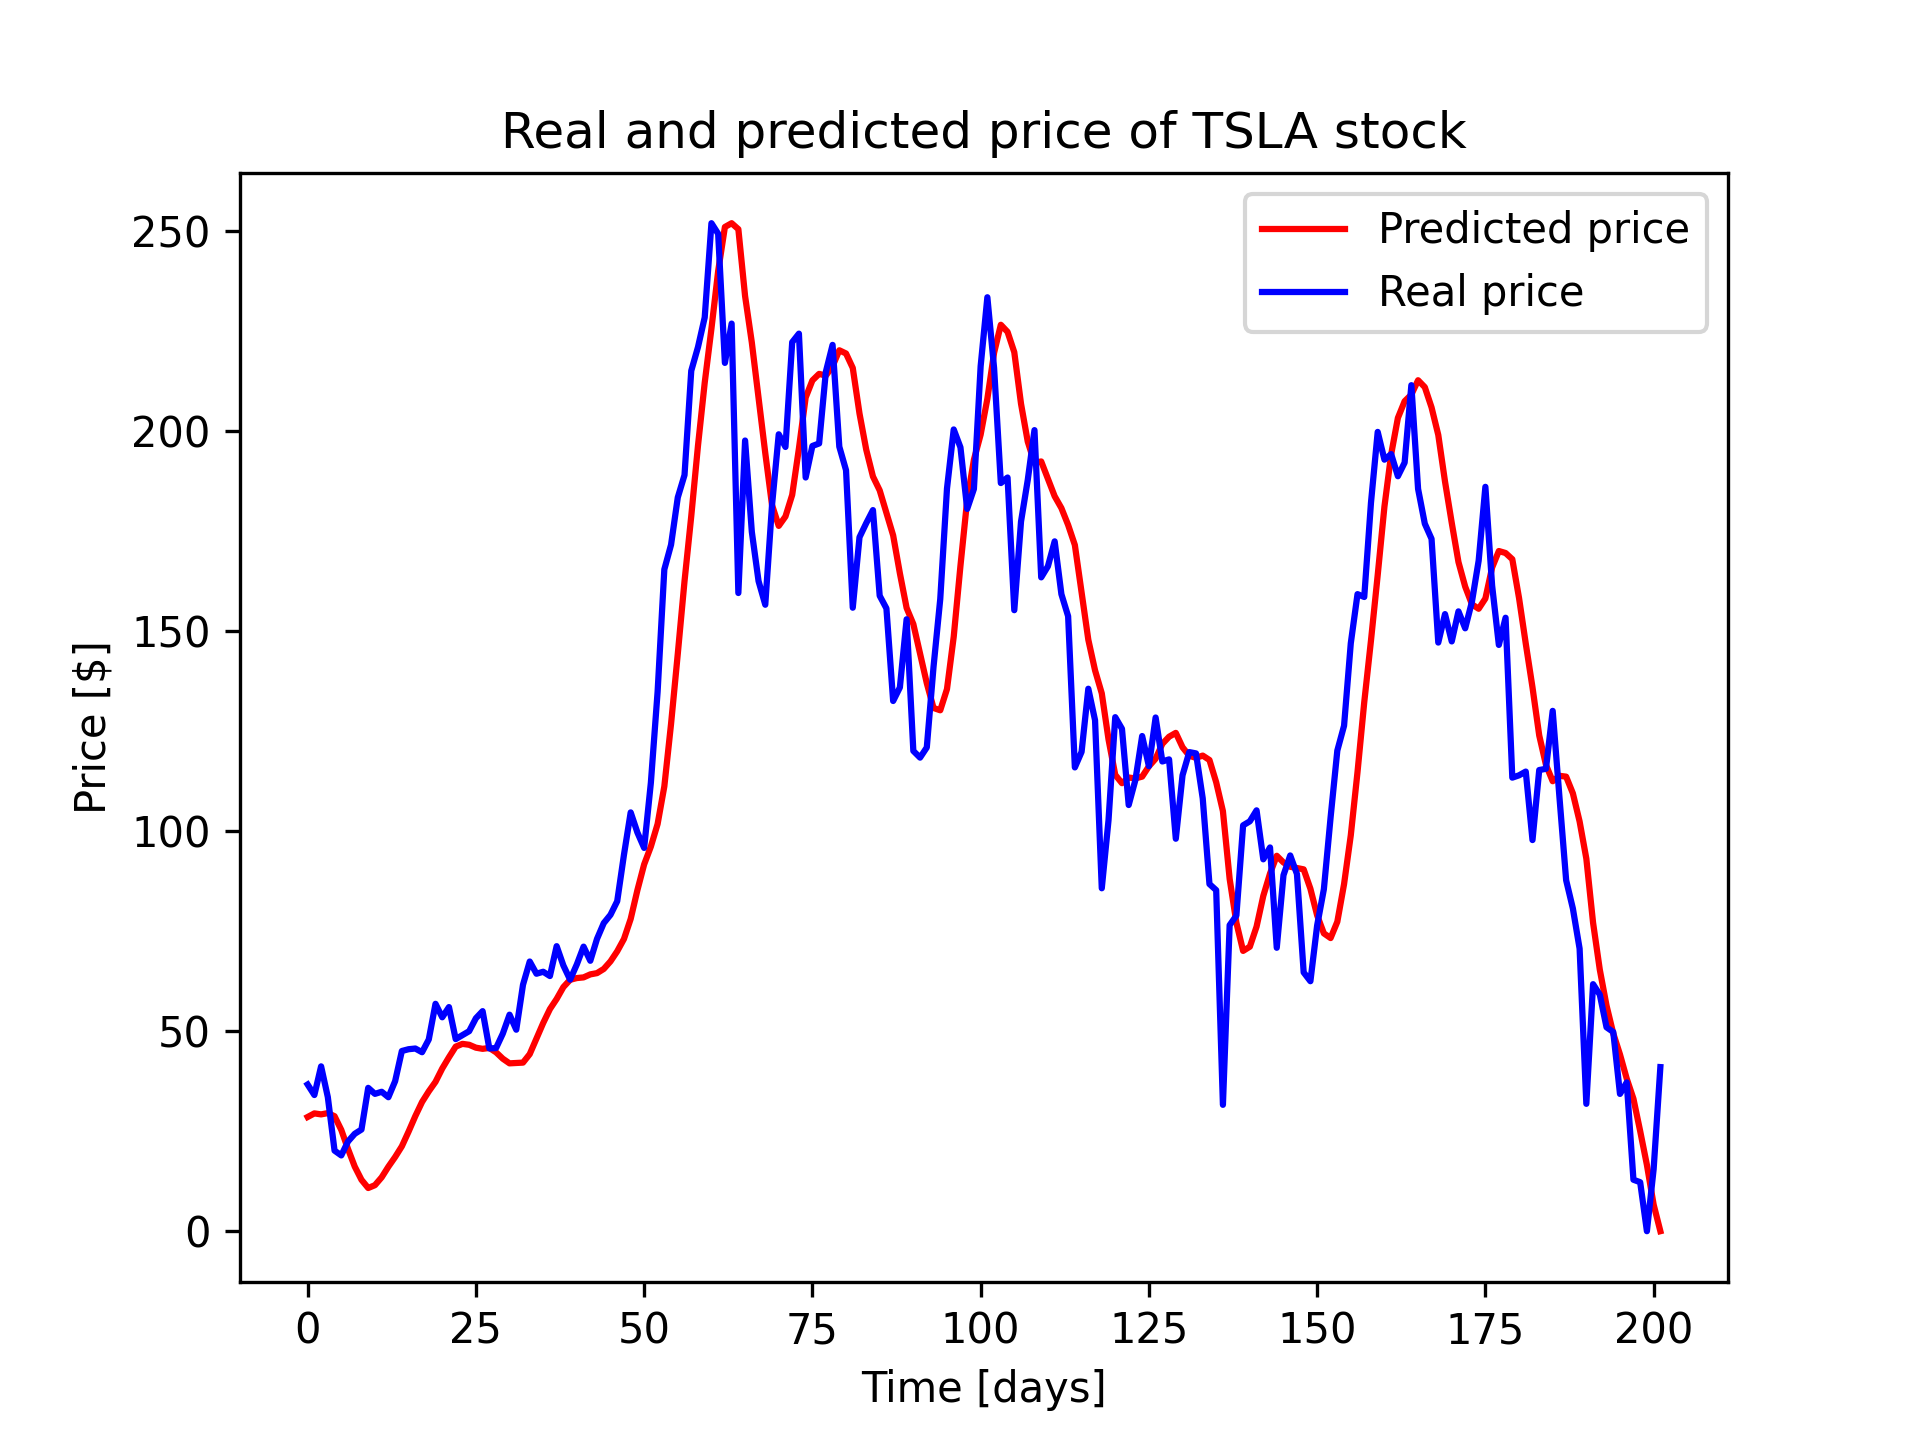
\includegraphics[width=0.5\textwidth]{./graf/model4/TSLA.png}
\caption{Real and predicted prices of the fourth model.}
\label{fig:label}
\end{figure} 

\clearpage
\subsection{Model 5}

Model5 - chunkSize: 50, time interval: 1 year, epochs: 10, trained on AAPL\par\bigskip
In this model, the lines showing the real price fluctuations and the price expected on the
market coincide in many areas. They show a systematic upward trend and a systematic decrease in
prices. However, it should be noted that sudden deflections were not depicted here by the course of
the red line. The red line does not reach its apogee if the deflection amplitude is large and sudden.
\par\bigskip
loss: 0.0076959822326898575\par
RMSE for AAPL equals 8.451018847518613\par
RMSE for AMZN equals 6.3281257280190095\par
RMSE for GOOGL equals 7.812833760162142\par
RMSE for LYFT equals 1.5628933553765902\par
RMSE for NVDA equals 6.9396920771979955\par
RMSE for TSLA equals 2.5031877336406927\par

\begin{figure}
% \centering
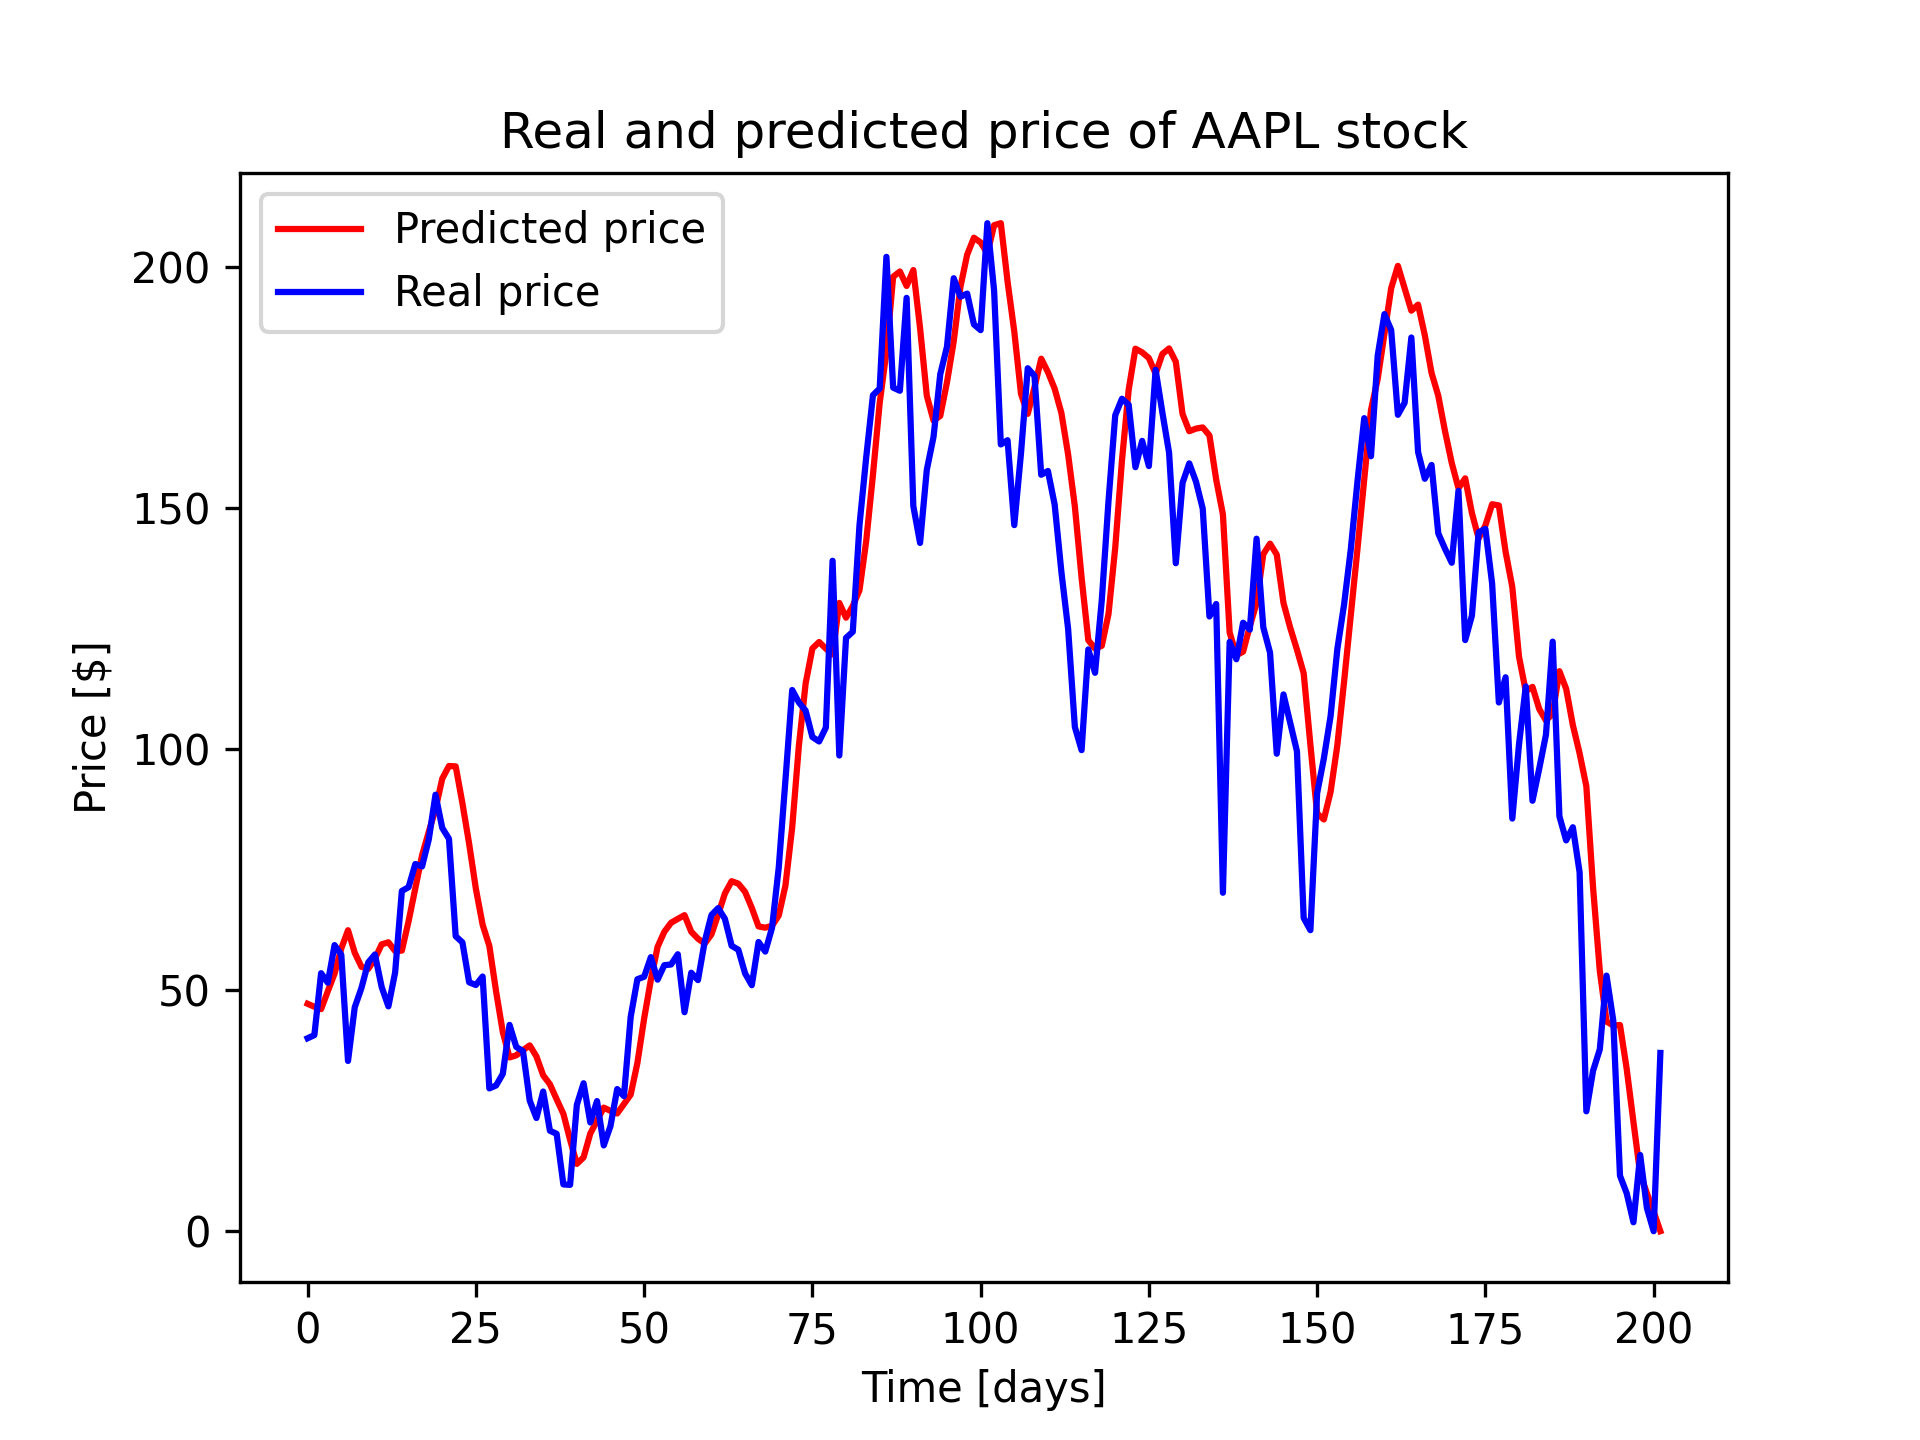
\includegraphics[width=0.5\textwidth]{./graf/model5/AAPL.png}
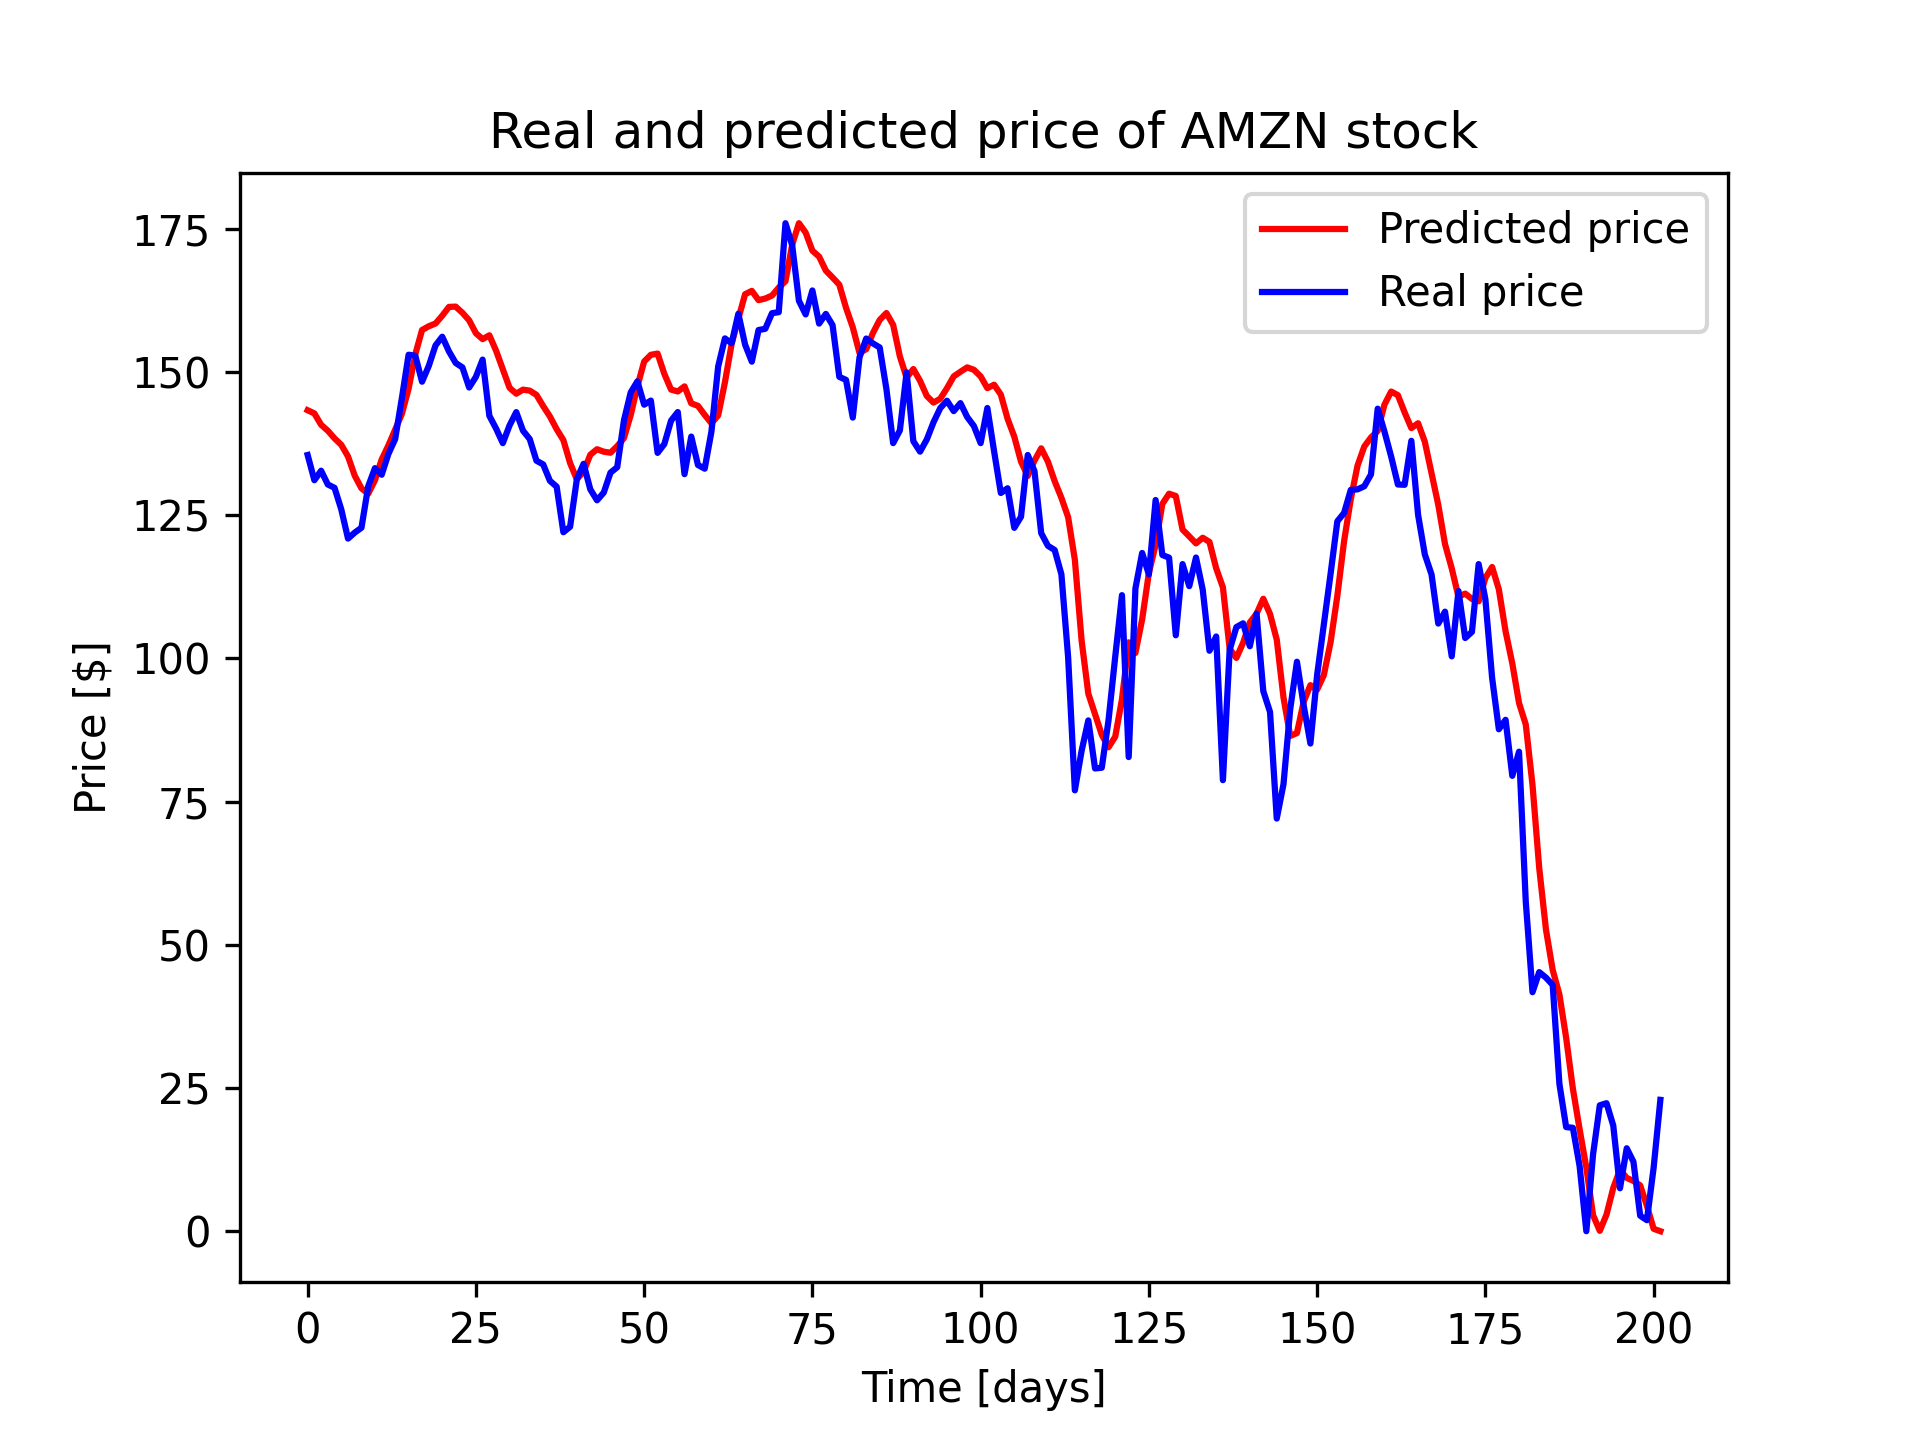
\includegraphics[width=0.5\textwidth]{./graf/model5/AMZN.png}
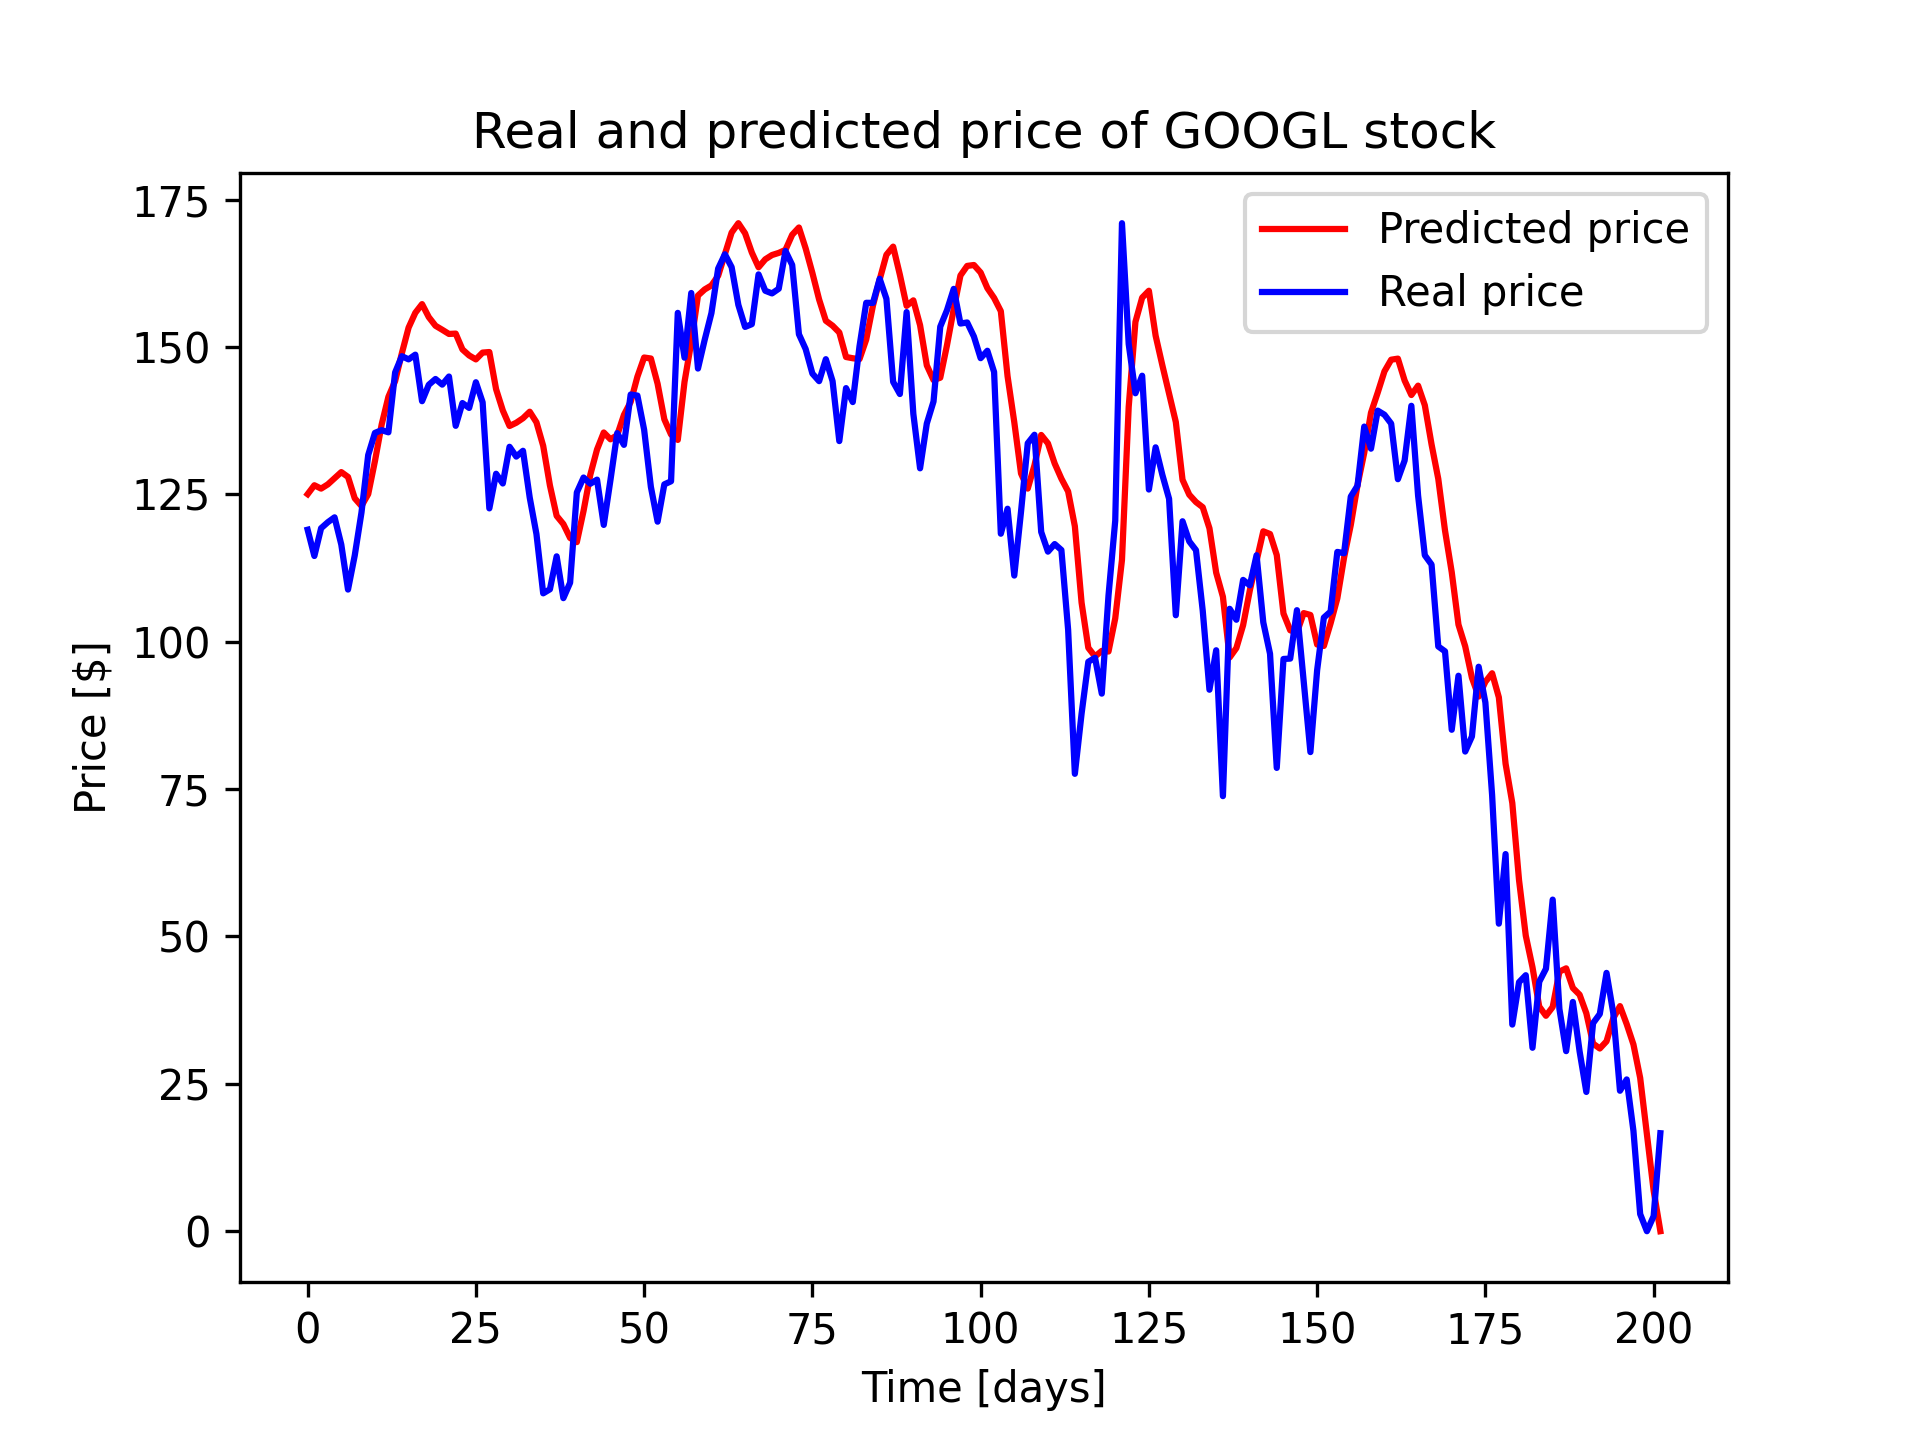
\includegraphics[width=0.5\textwidth]{./graf/model5/GOOGL.png}
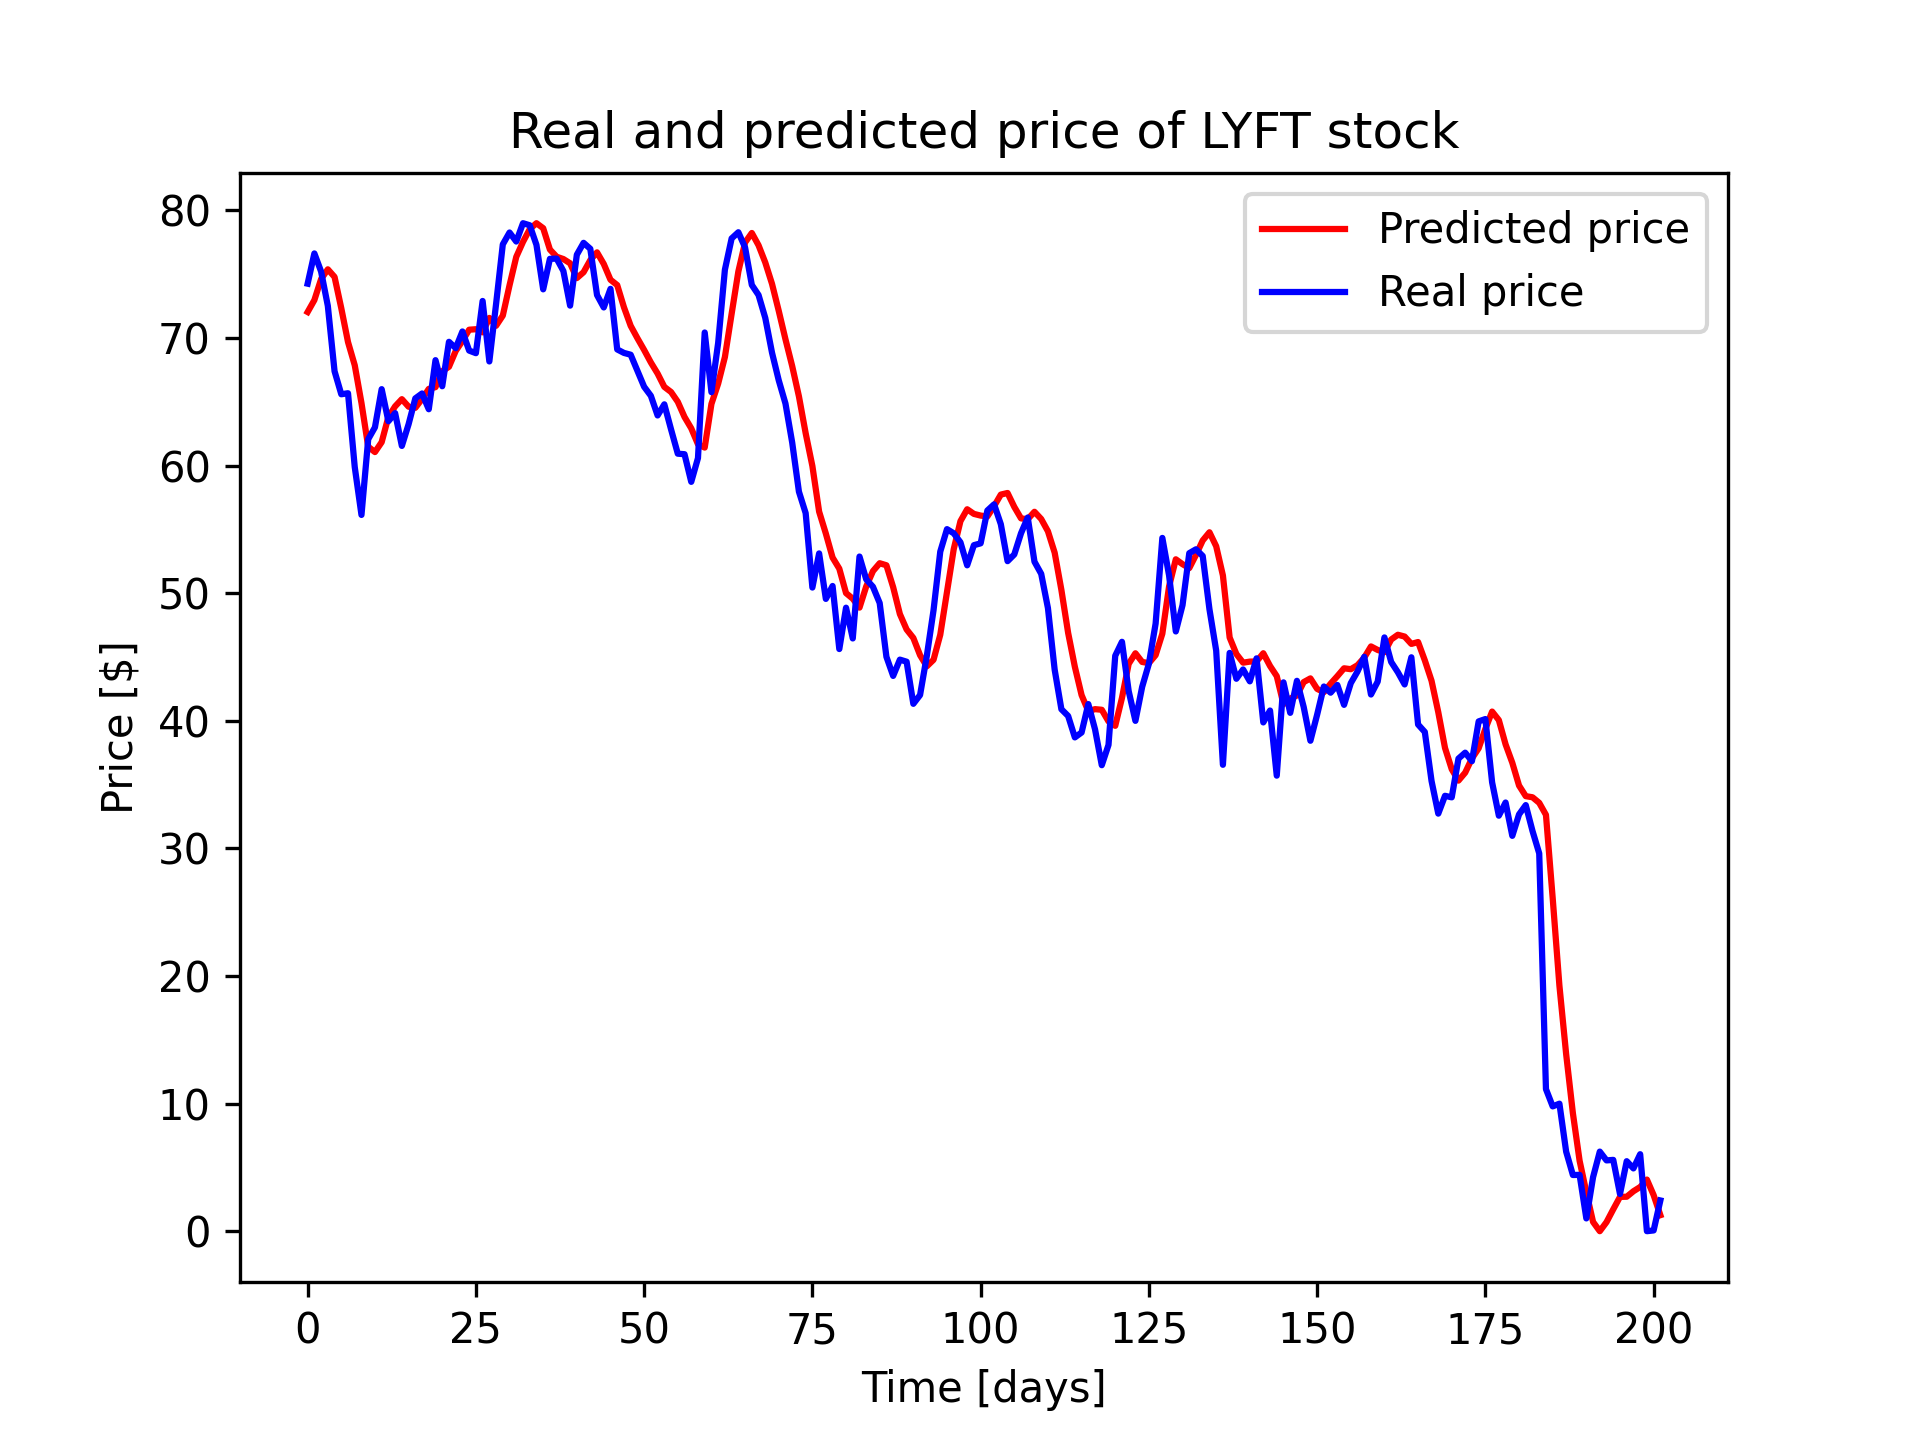
\includegraphics[width=0.5\textwidth]{./graf/model5/LYFT.png}
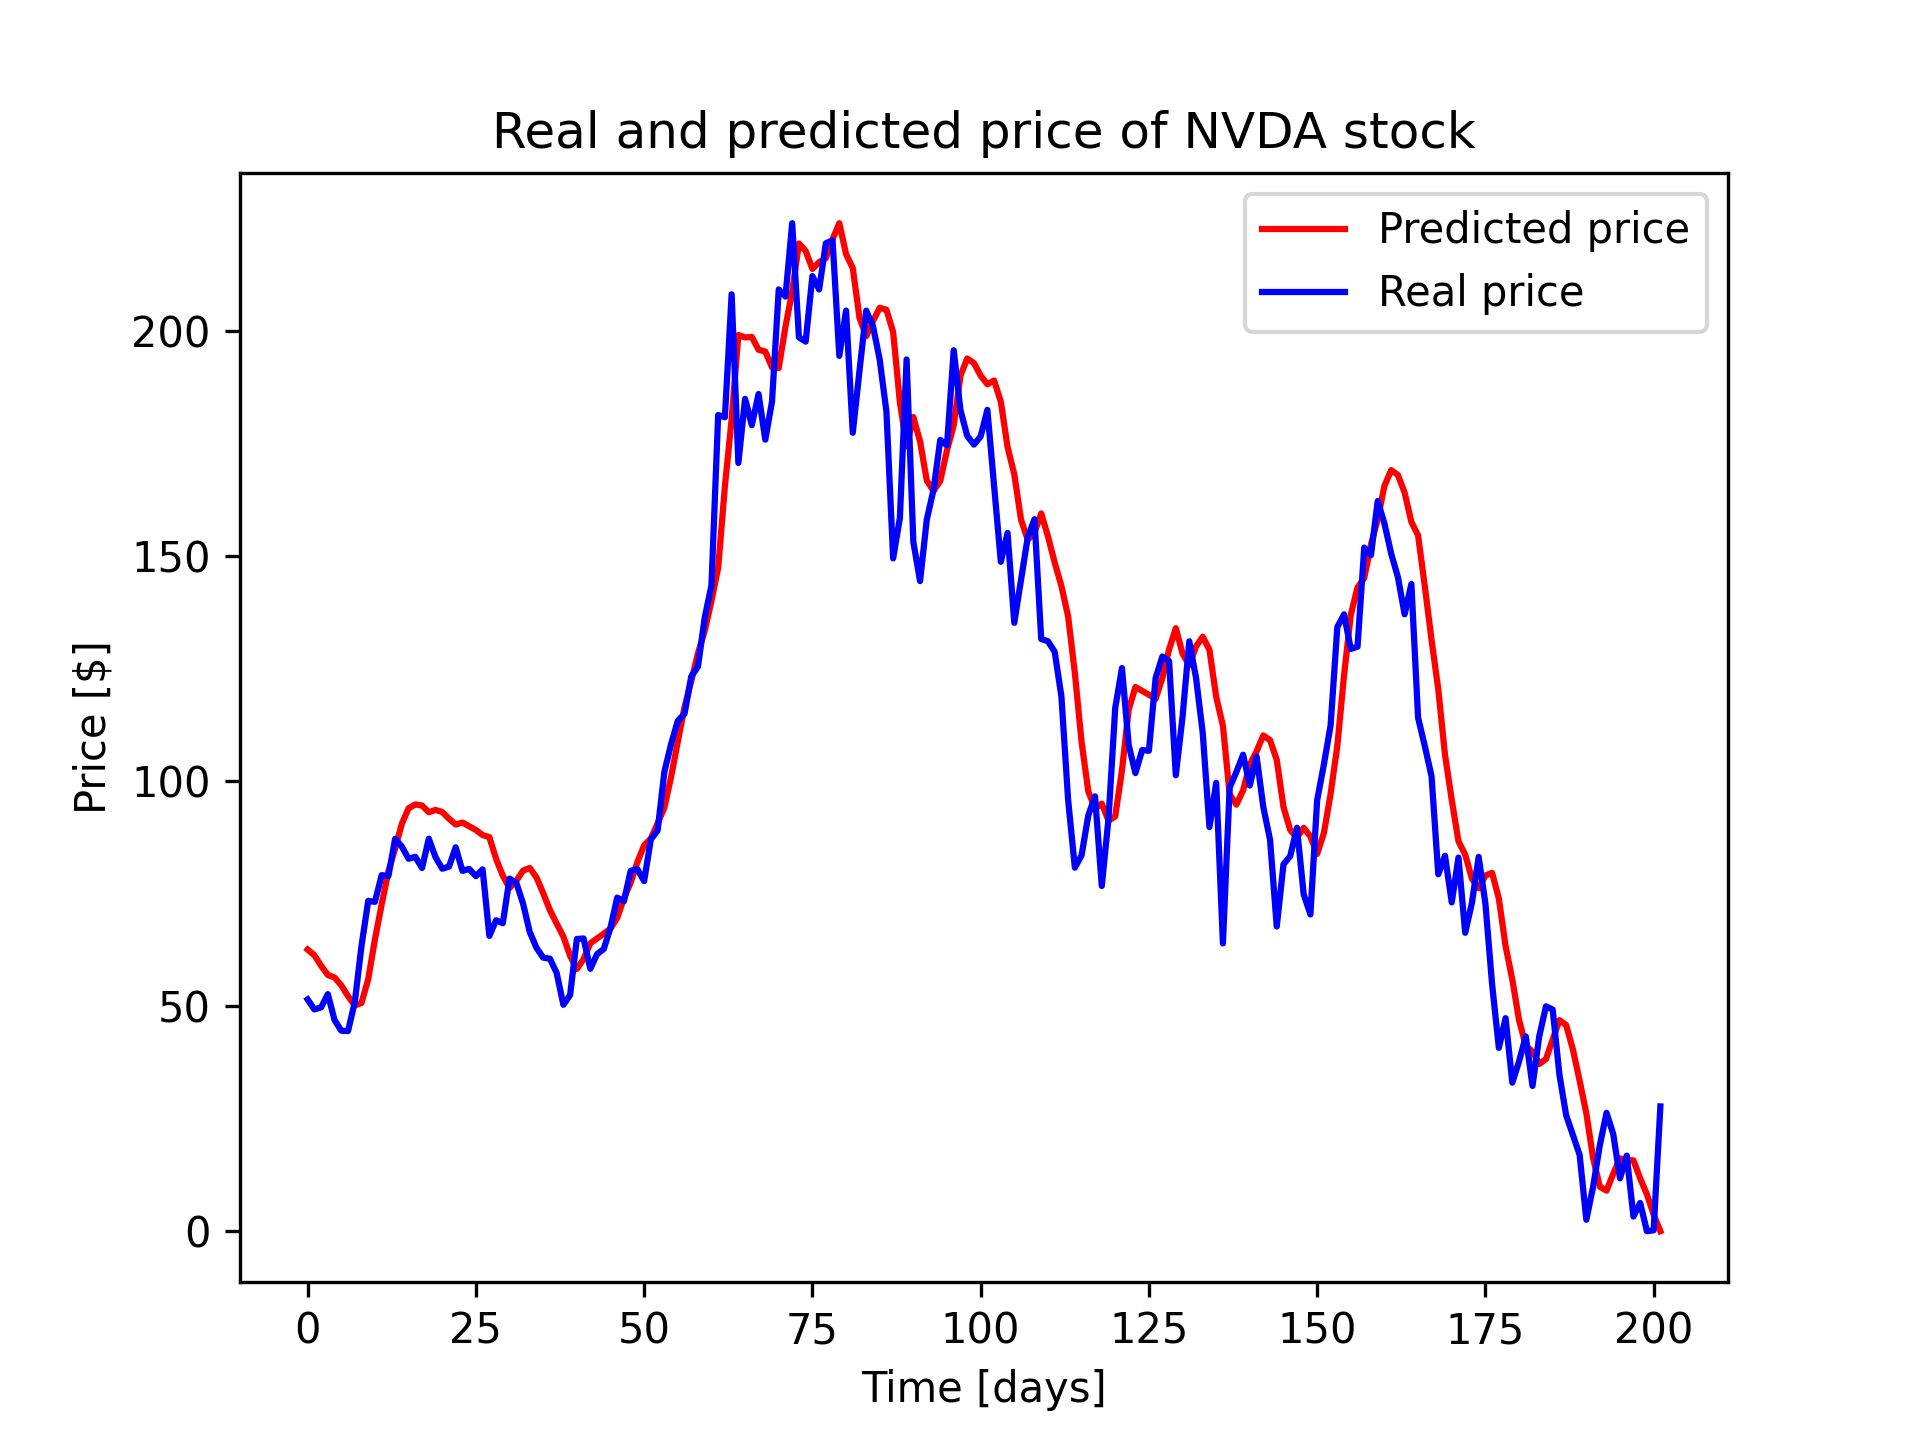
\includegraphics[width=0.5\textwidth]{./graf/model5/NVDA.png}
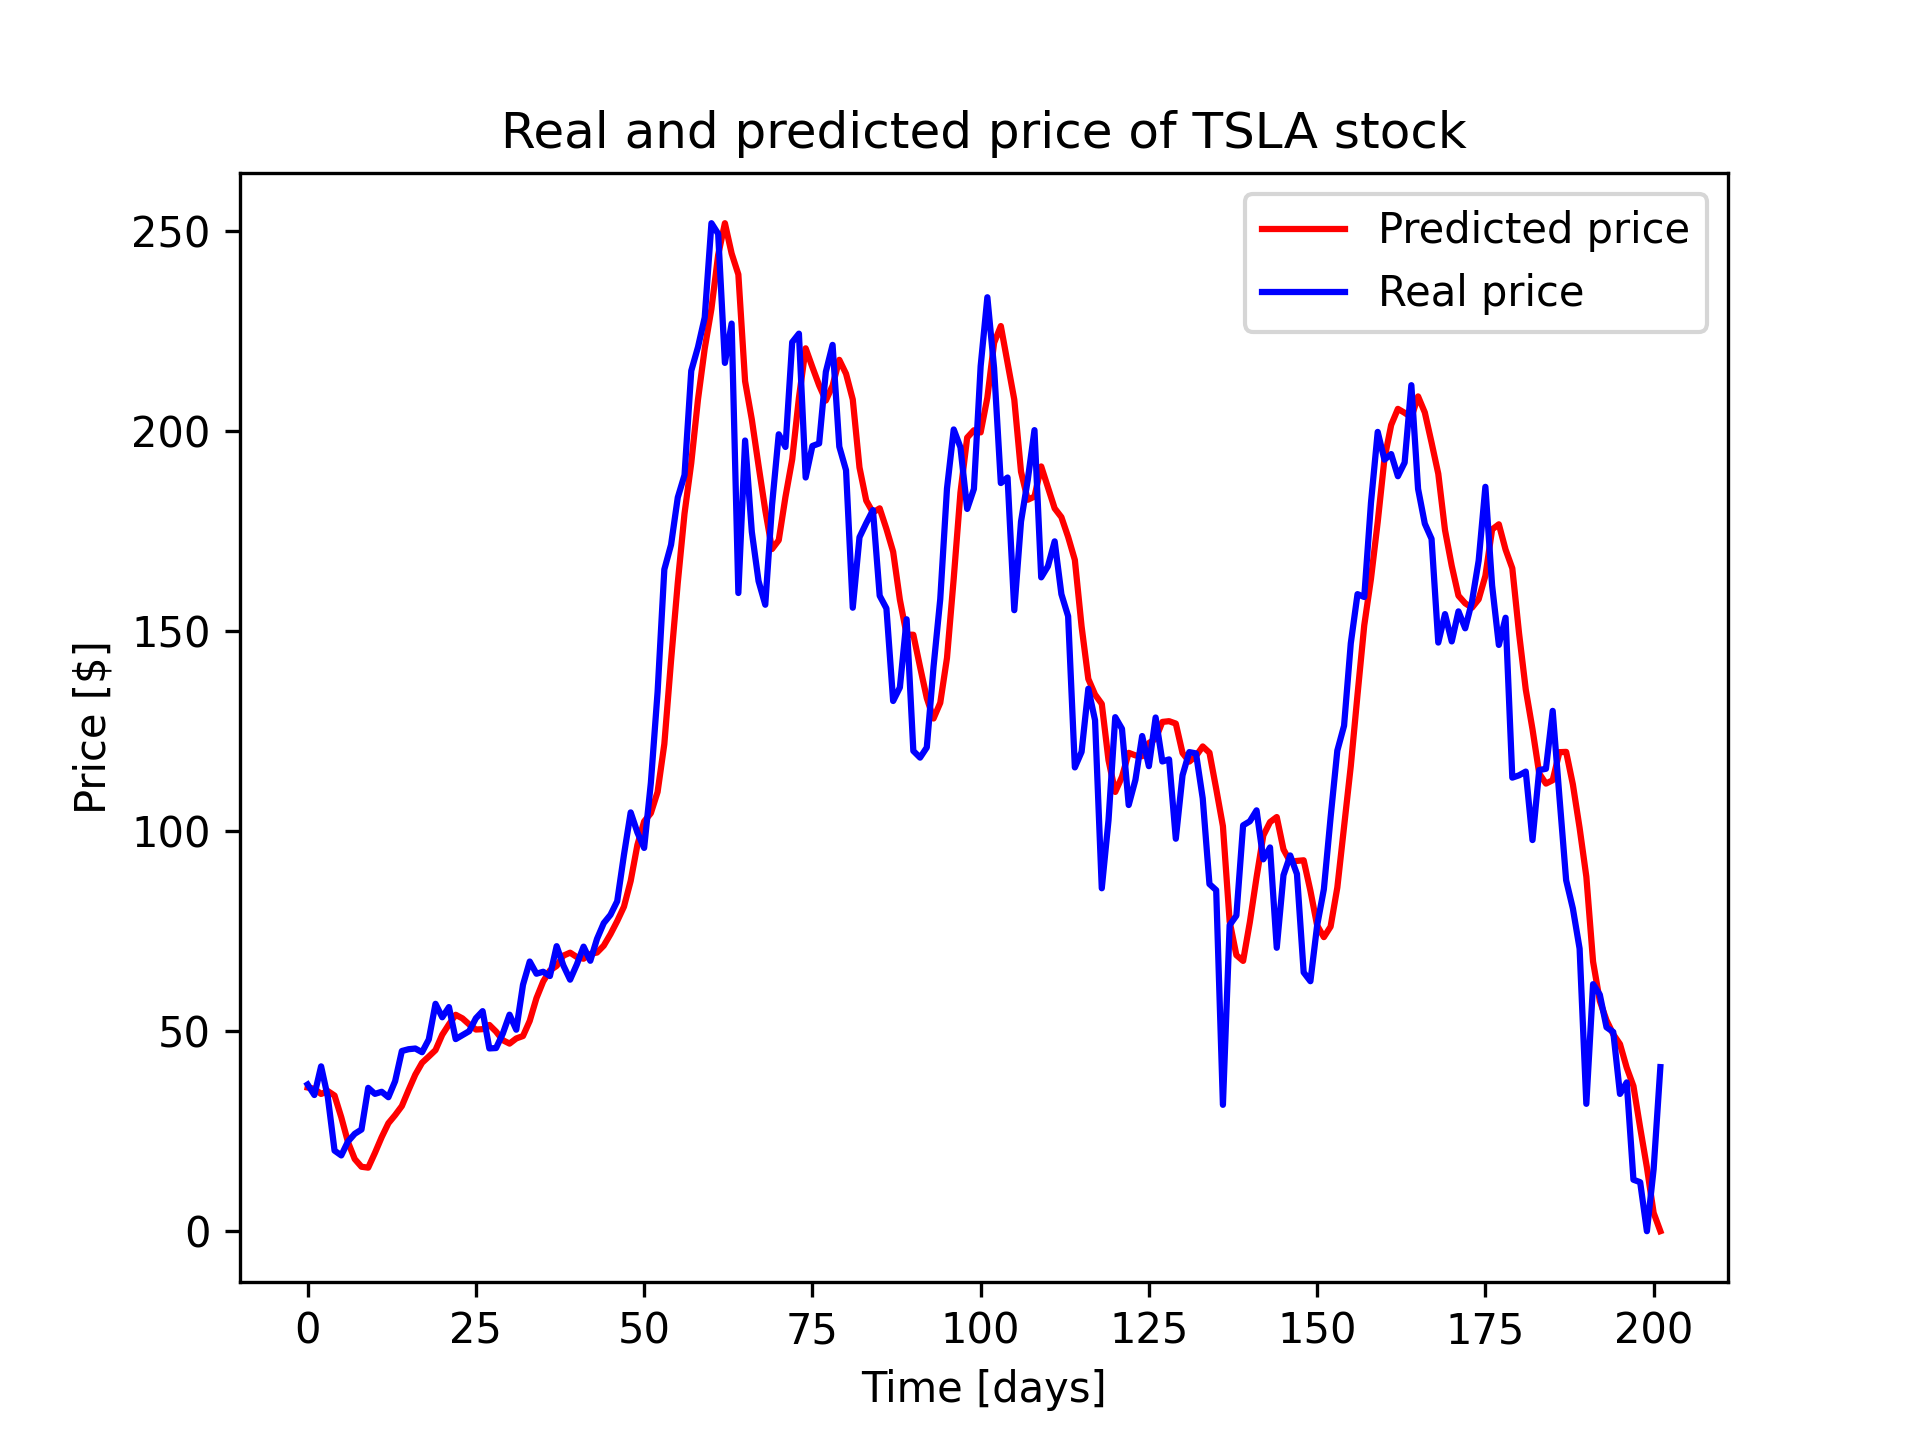
\includegraphics[width=0.5\textwidth]{./graf/model5/TSLA.png}
\caption{Real and predicted prices of the fifth model.}
\label{fig:label}
\end{figure} 

\clearpage
\subsection{Model 6}

Model6 - chunkSize: 50, time interval: 1 year, epochs: 15, trained on AAPL\par\bigskip
Observing the deflections of the line in model 6, it can be observed that the course of both lines does
not always coincide over their entire course. Analyzing the path of the red line, it can be seen that it
runs above the blue line. Given the horizontal shift, it runs to the right of the blue line. When
considering situations where prices go up or down systematically, both lines coincide, which is worth
noting. On the other hand, sudden price drops shown in the blue line are not reflected in the course
of the red line. This situation is most marked in the graph for AAPL.png., and GOOGL.png.
\par\bigskip
loss: 0.007239694241434336\par
RMSE for AAPL equals 9.205821423904716\par
RMSE for AMZN equals 6.248347468675569\par
RMSE for GOOGL equals 9.552054273137703\par
RMSE for LYFT equals 2.1290812183842194\par
RMSE for NVDA equals 8.775806702137338\par
RMSE for TSLA equals 5.196206788544533\par

\begin{figure}
% \centering
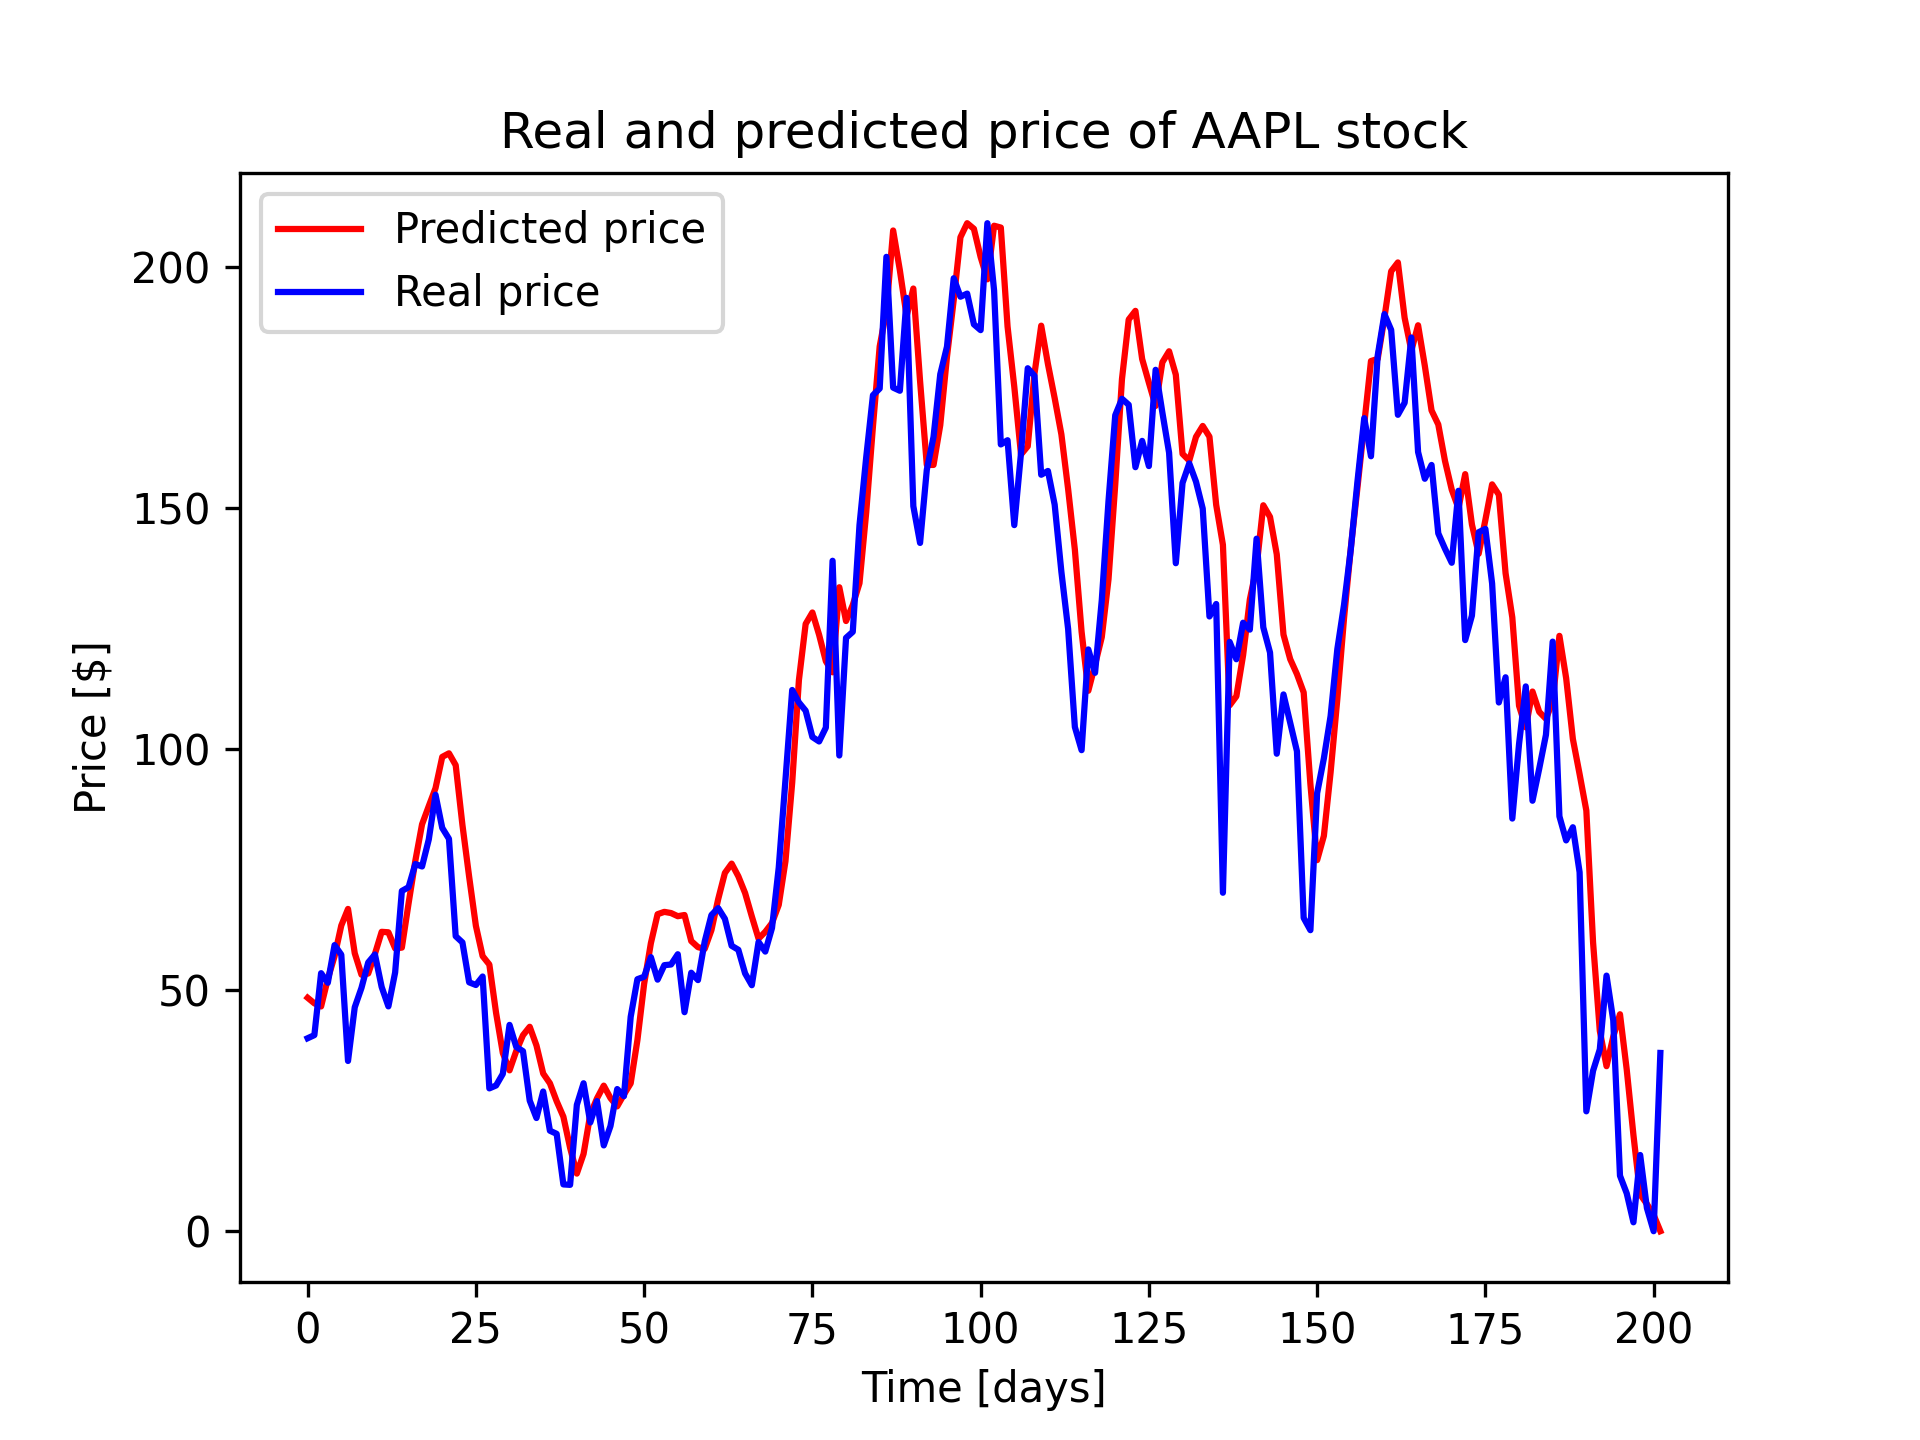
\includegraphics[width=0.5\textwidth]{./graf/model6/AAPL.png}
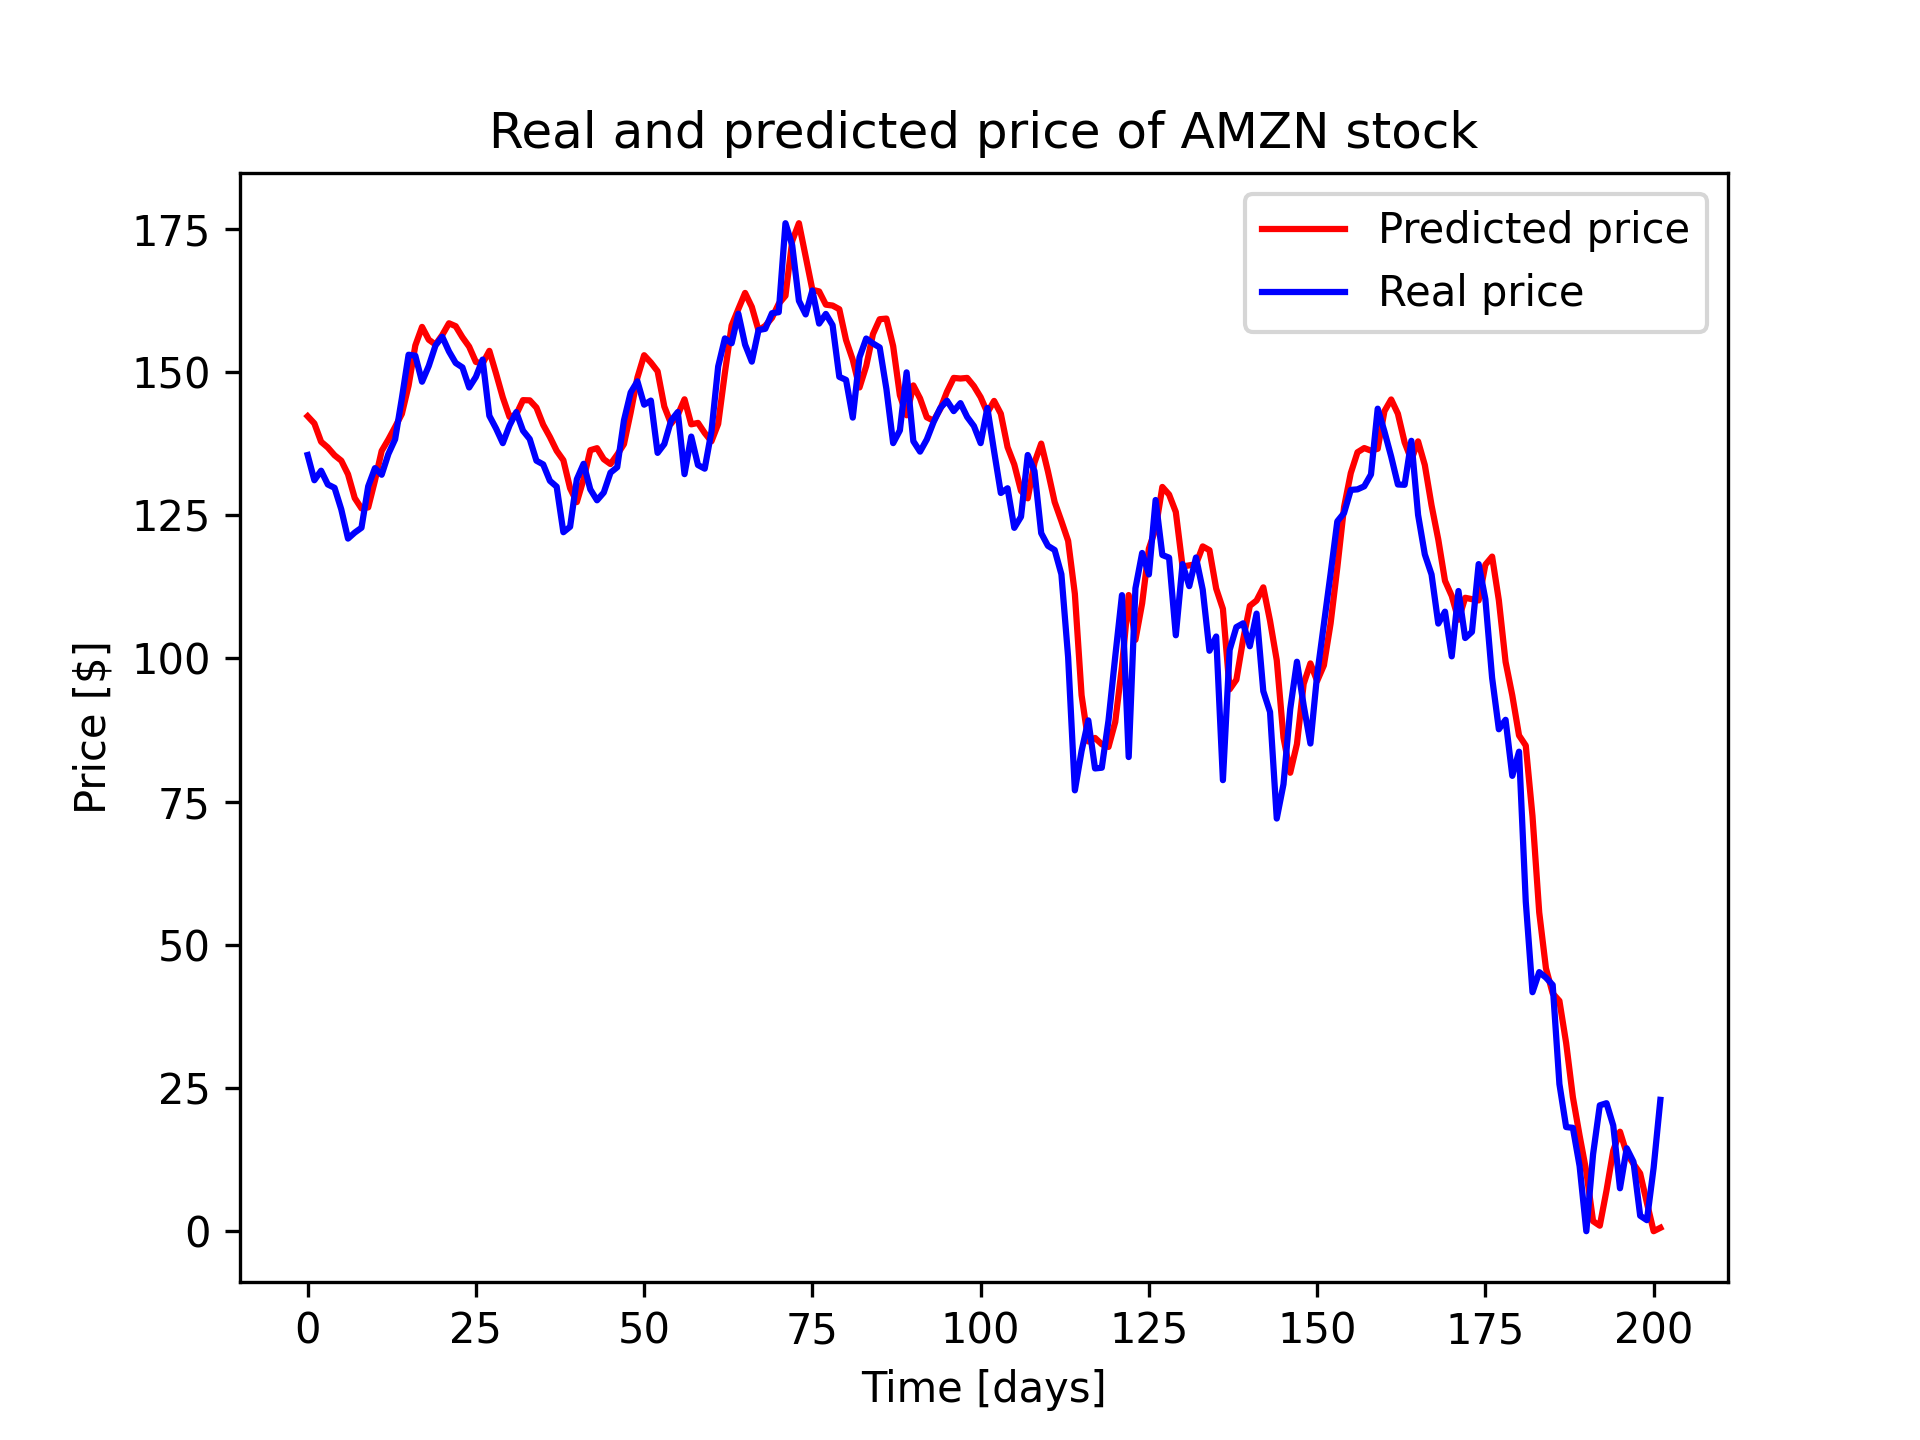
\includegraphics[width=0.5\textwidth]{./graf/model6/AMZN.png}
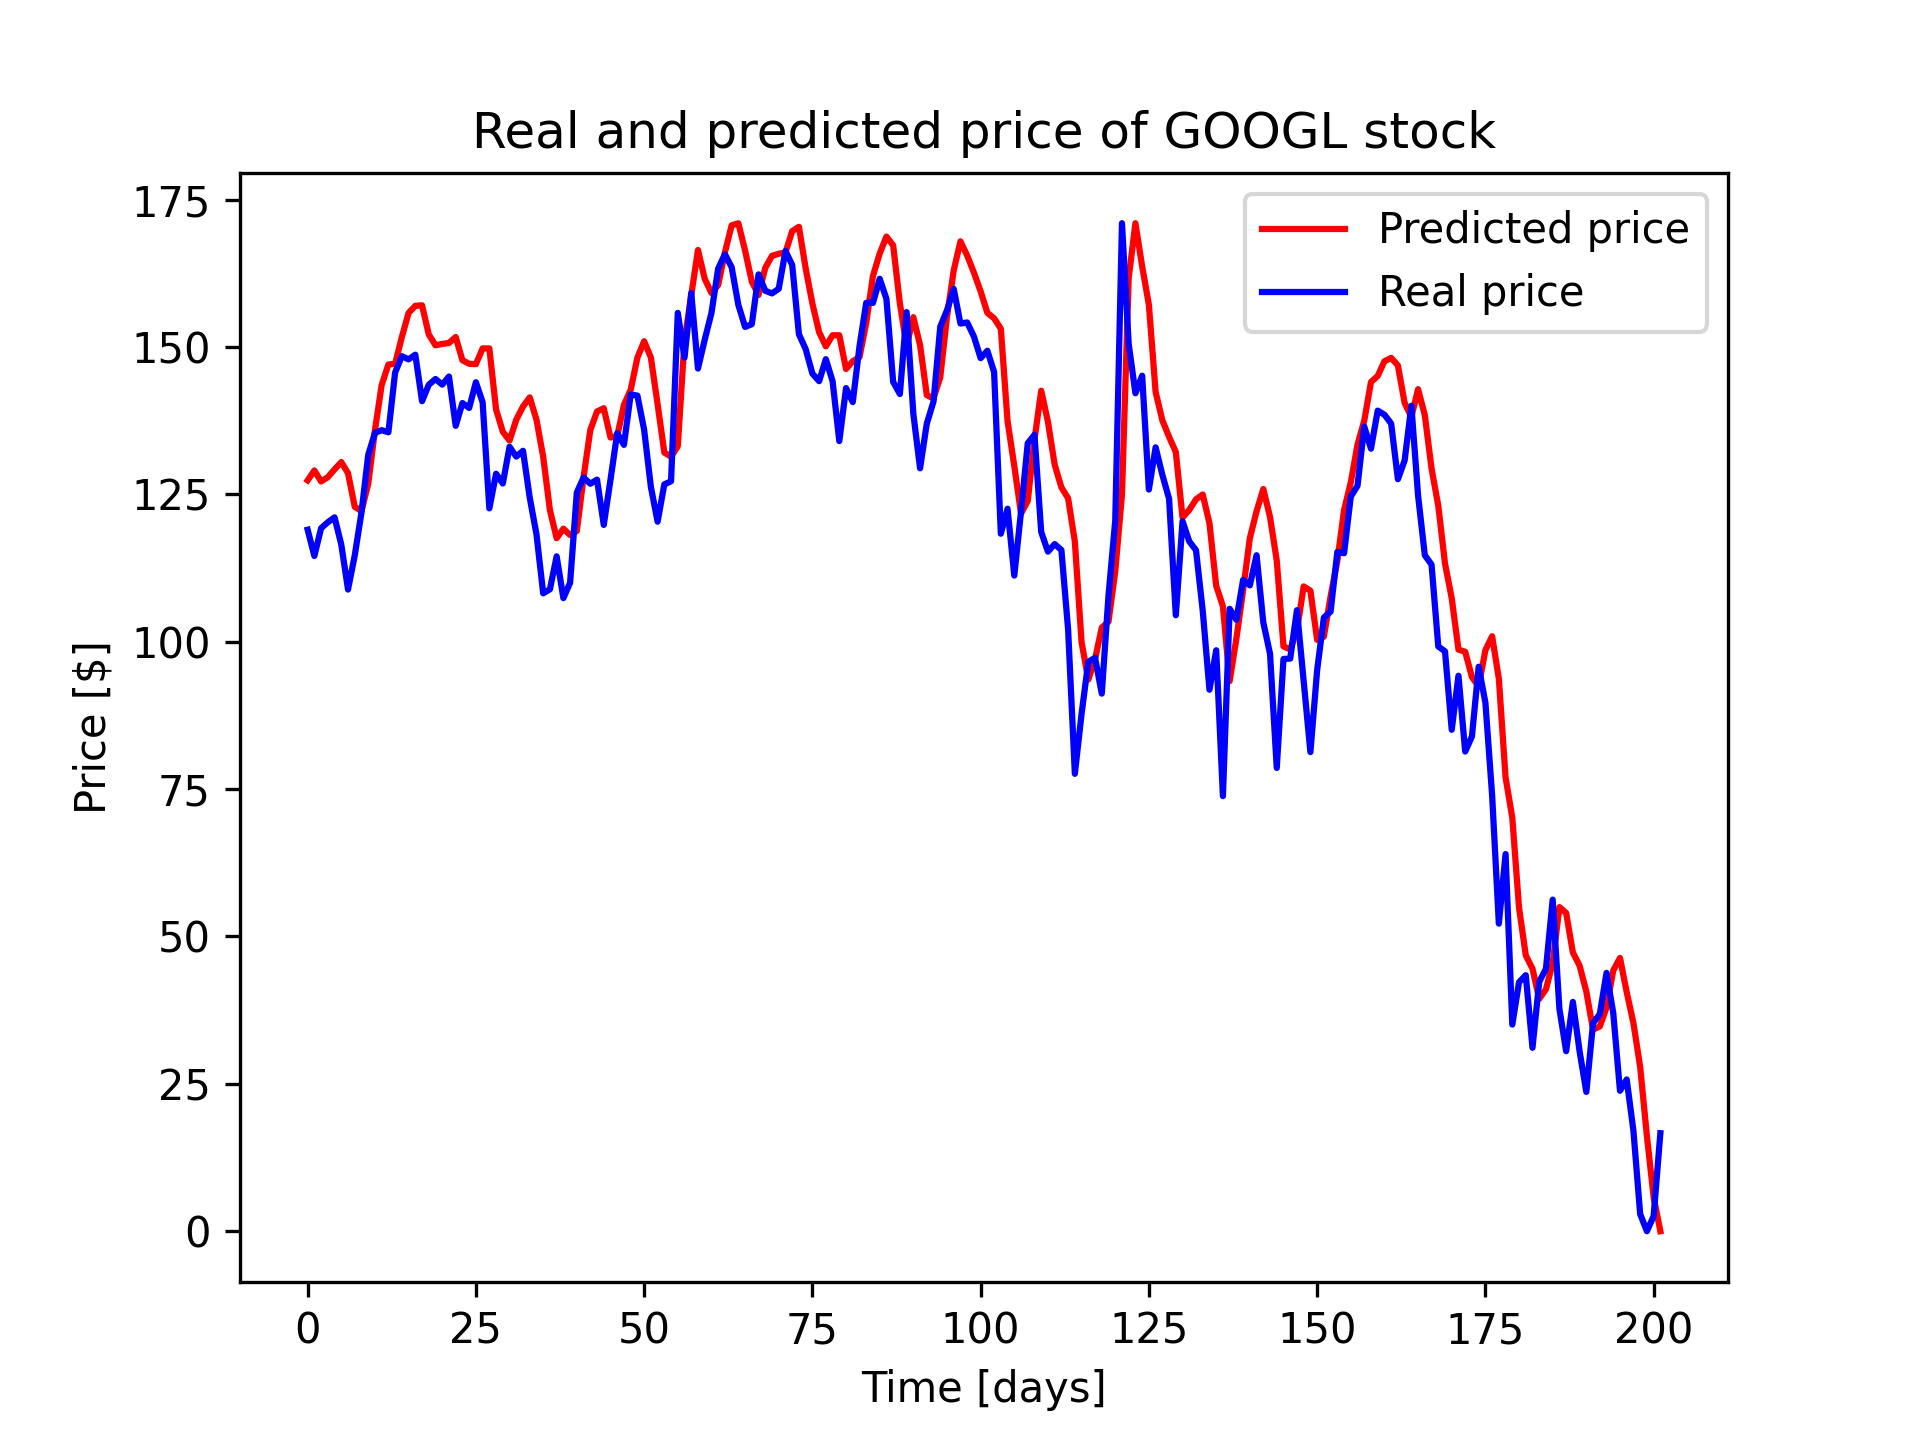
\includegraphics[width=0.5\textwidth]{./graf/model6/GOOGL.png}
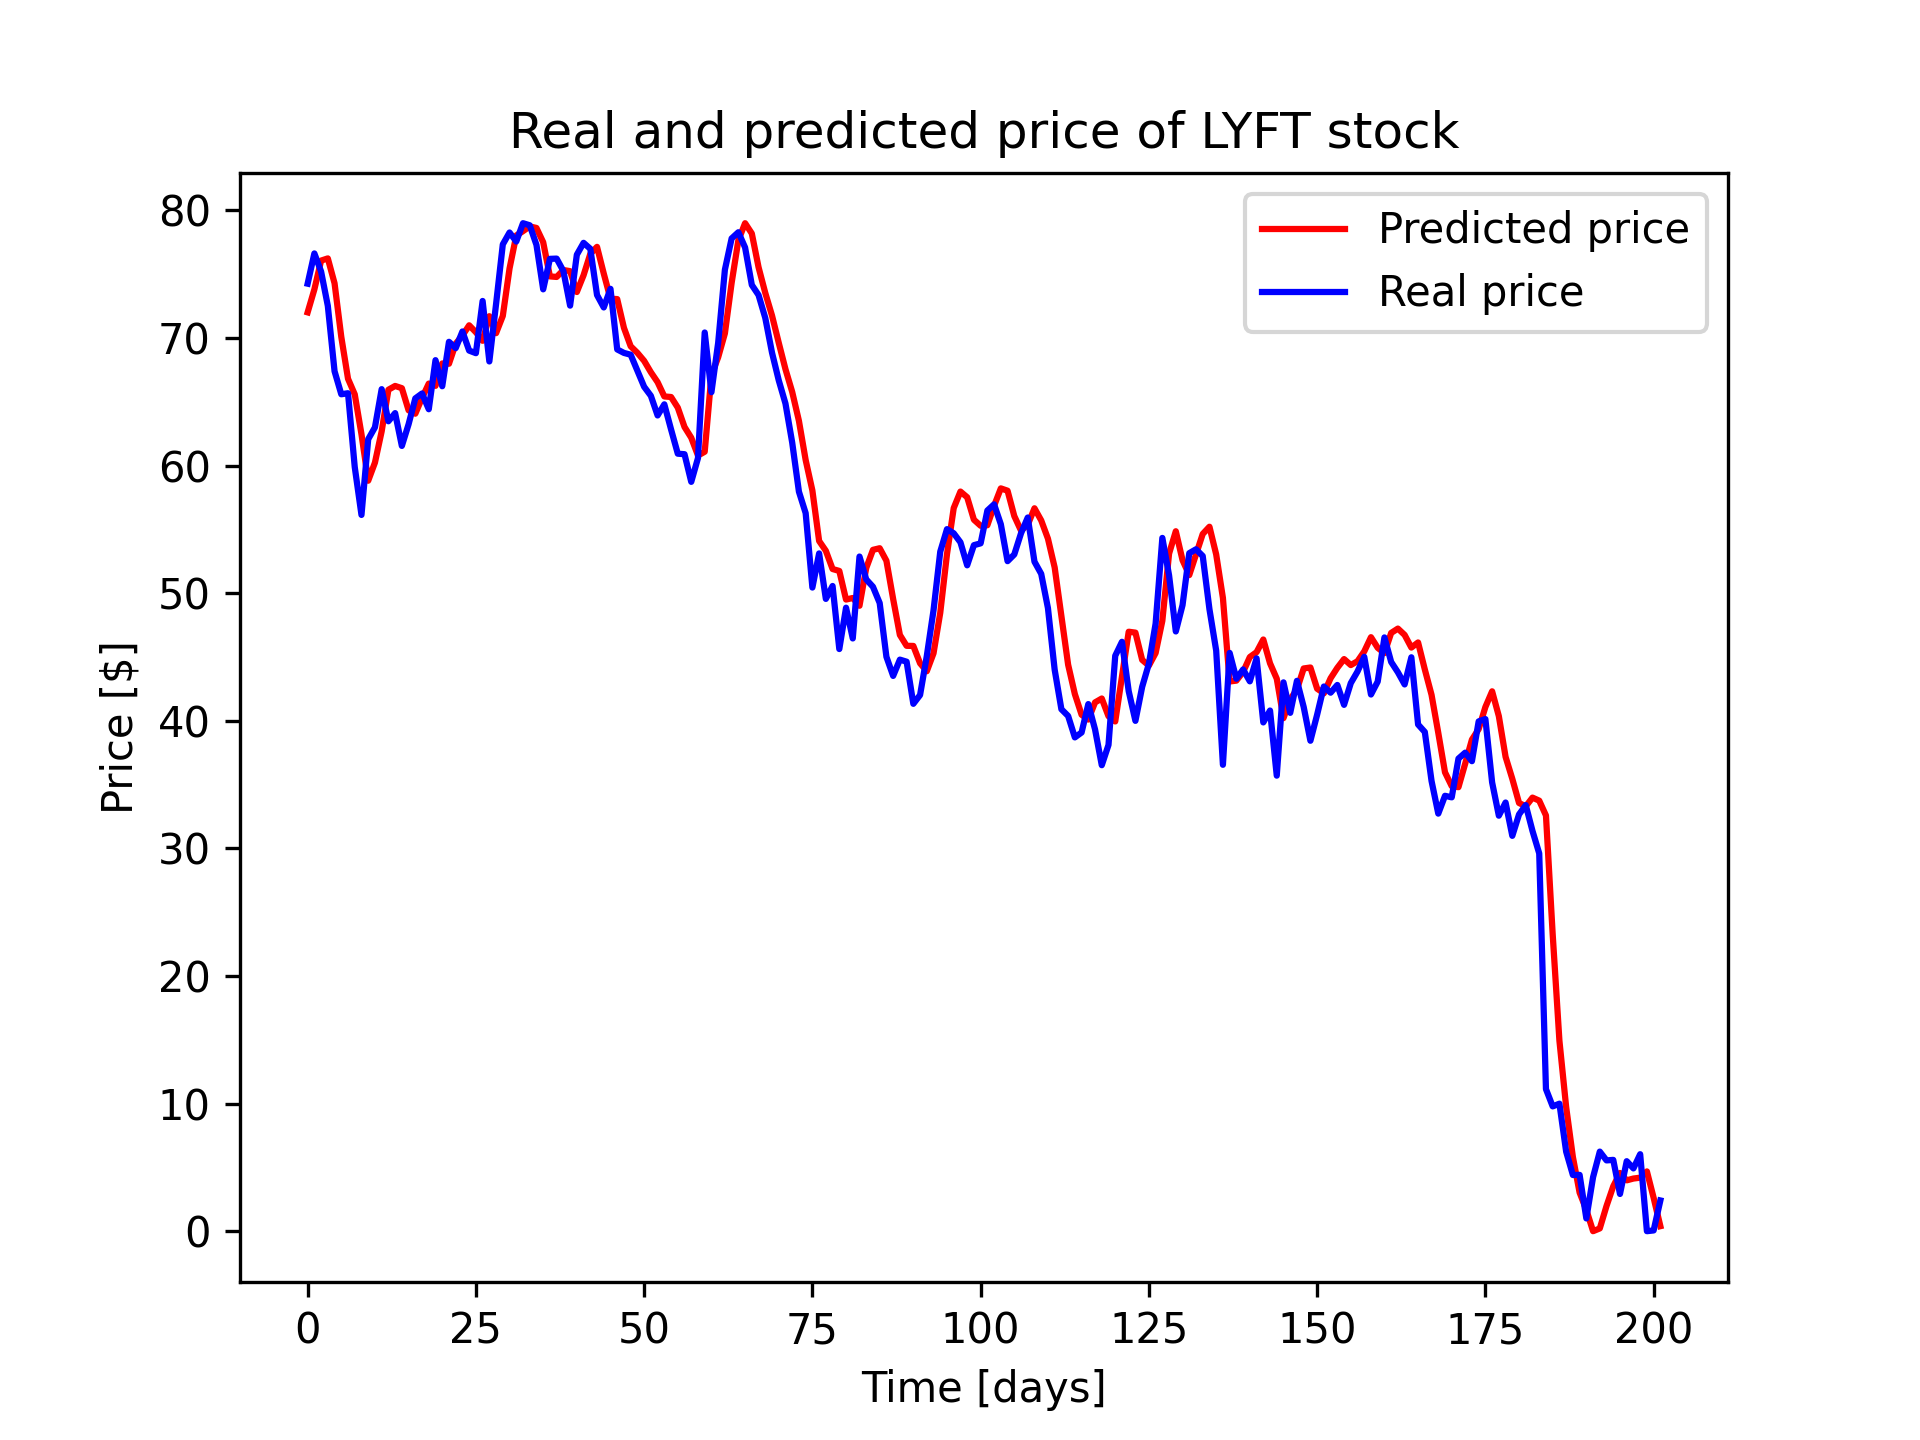
\includegraphics[width=0.5\textwidth]{./graf/model6/LYFT.png}
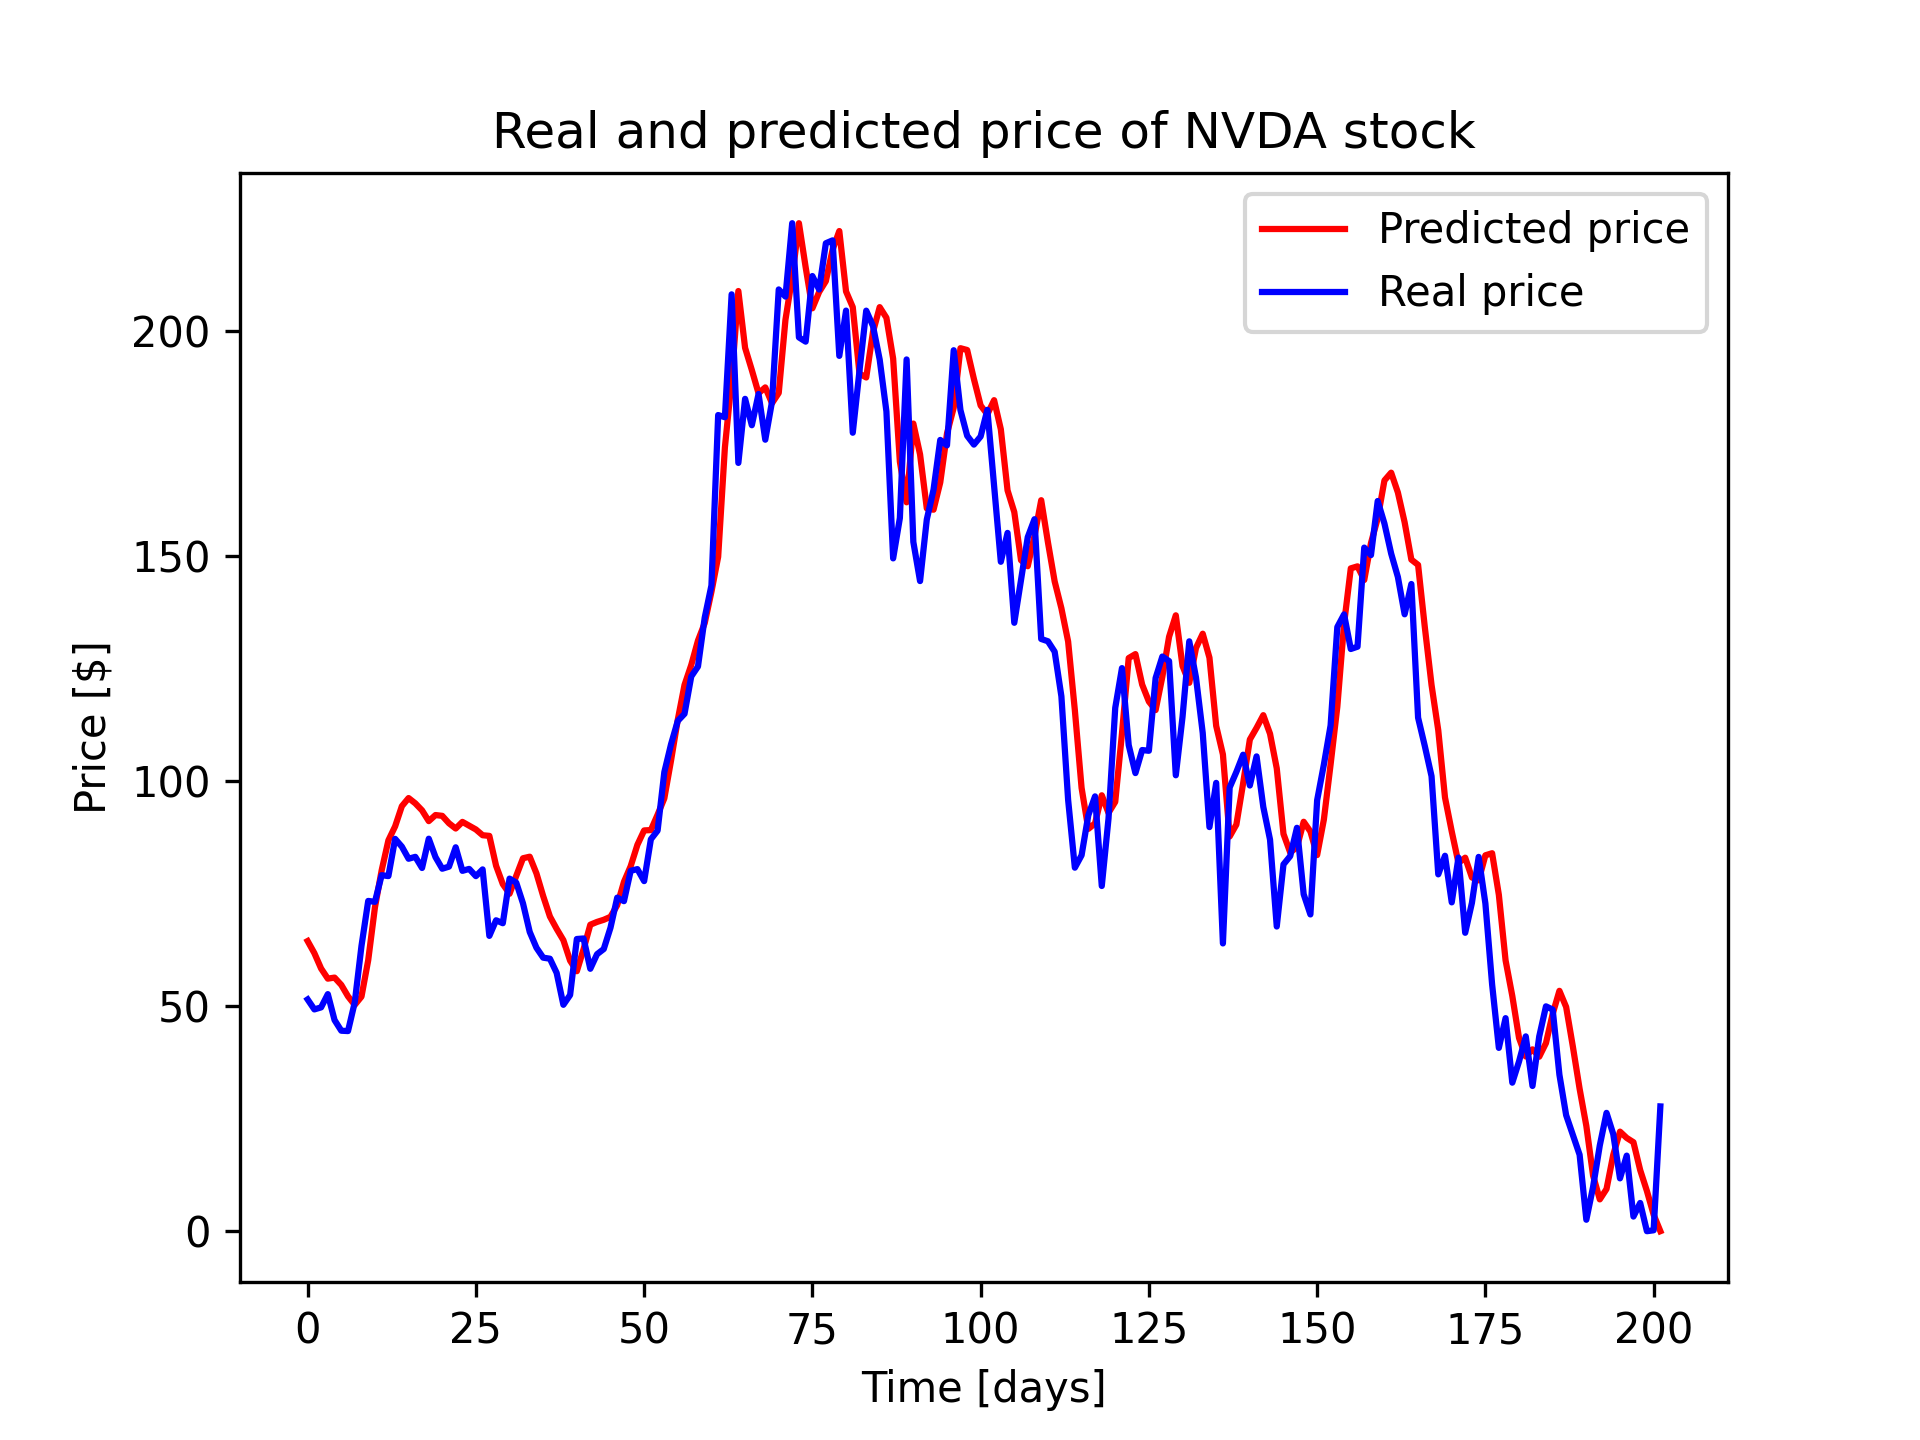
\includegraphics[width=0.5\textwidth]{./graf/model6/NVDA.png}
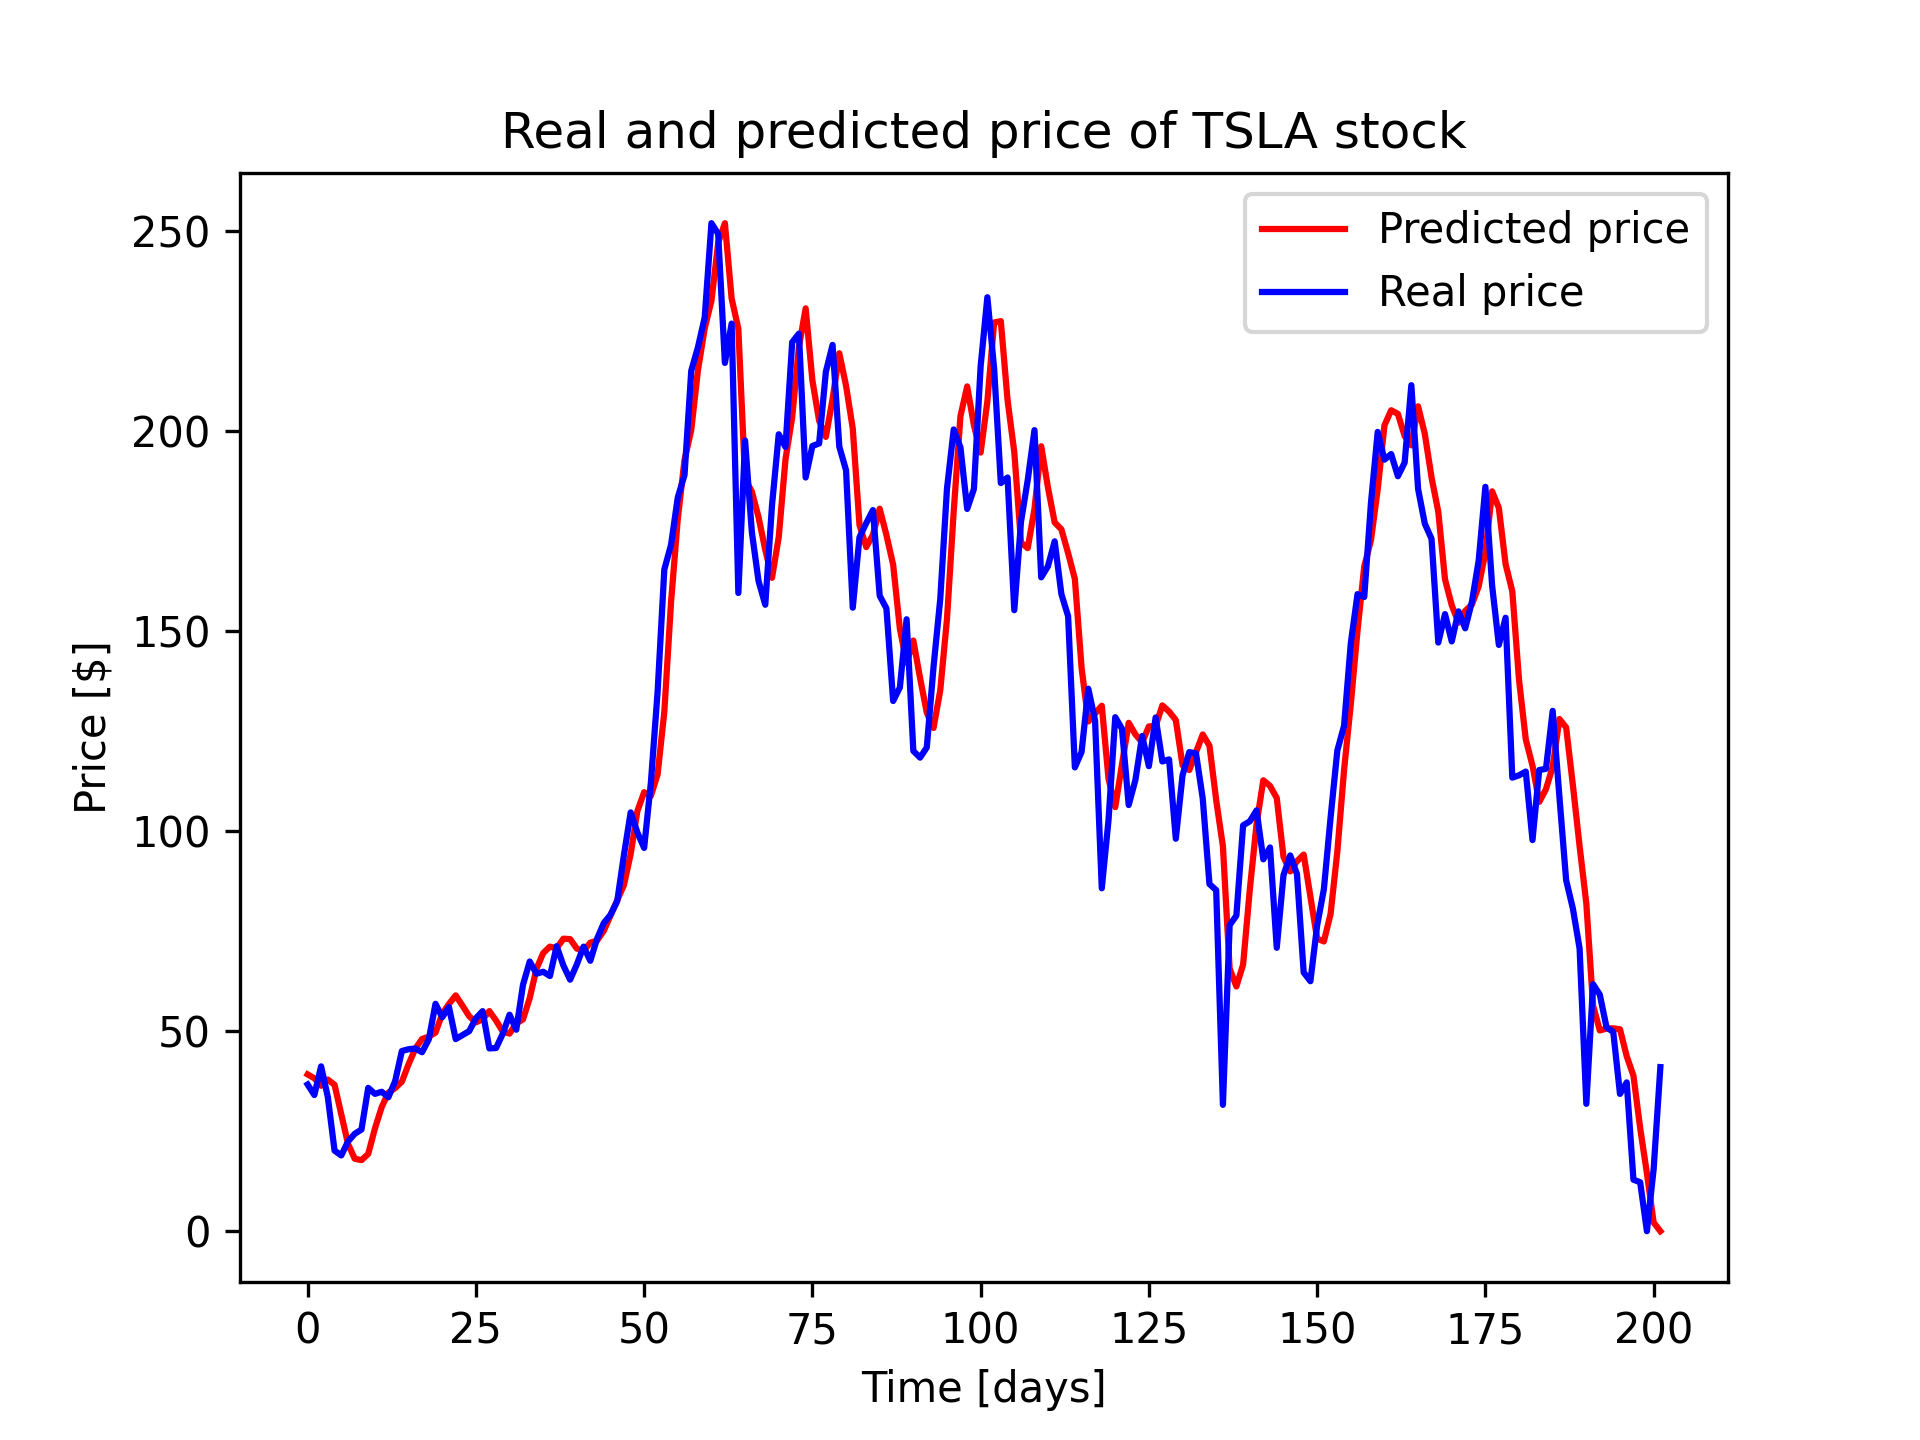
\includegraphics[width=0.5\textwidth]{./graf/model6/TSLA.png}
\caption{Real and predicted prices of the sixth model.}
\label{fig:label}
\end{figure} 

\clearpage
\subsection{Model 7}

Model7 - chunkSize: 100, time interval: 1 year, epochs: 5, trained on AAPL\par\bigskip
In this model, when observing and analyzing the course of both lines, the first thing that can be
noticed is that the red line is too smooth concerning the blue line. The blue line has strongly
peaked peaks, while the red line is visibly smooth throughout its course. Only a mild increase or
decrease in prices is signaled. In this model, short-term price fluctuations were not marked on the
charts. Few-day discounts or increases are not reflected in the red line. Sudden, rapid
changes are not included in this model. In addition, the red line is significantly shifted to the right and
runs higher than the blue line for its entire length.
\par\bigskip
loss: 0.01530853658914566\par
RMSE for AAPL equals 8.821475143305953\par
RMSE for AMZN equals 8.298883063025912\par
RMSE for GOOGL equals 6.907164316613046\par
RMSE for LYFT equals 2.7909029046154528\par
RMSE for NVDA equals 7.455910063022197\par
RMSE for TSLA equals 5.396200631636798\par

\begin{figure}
% \centering
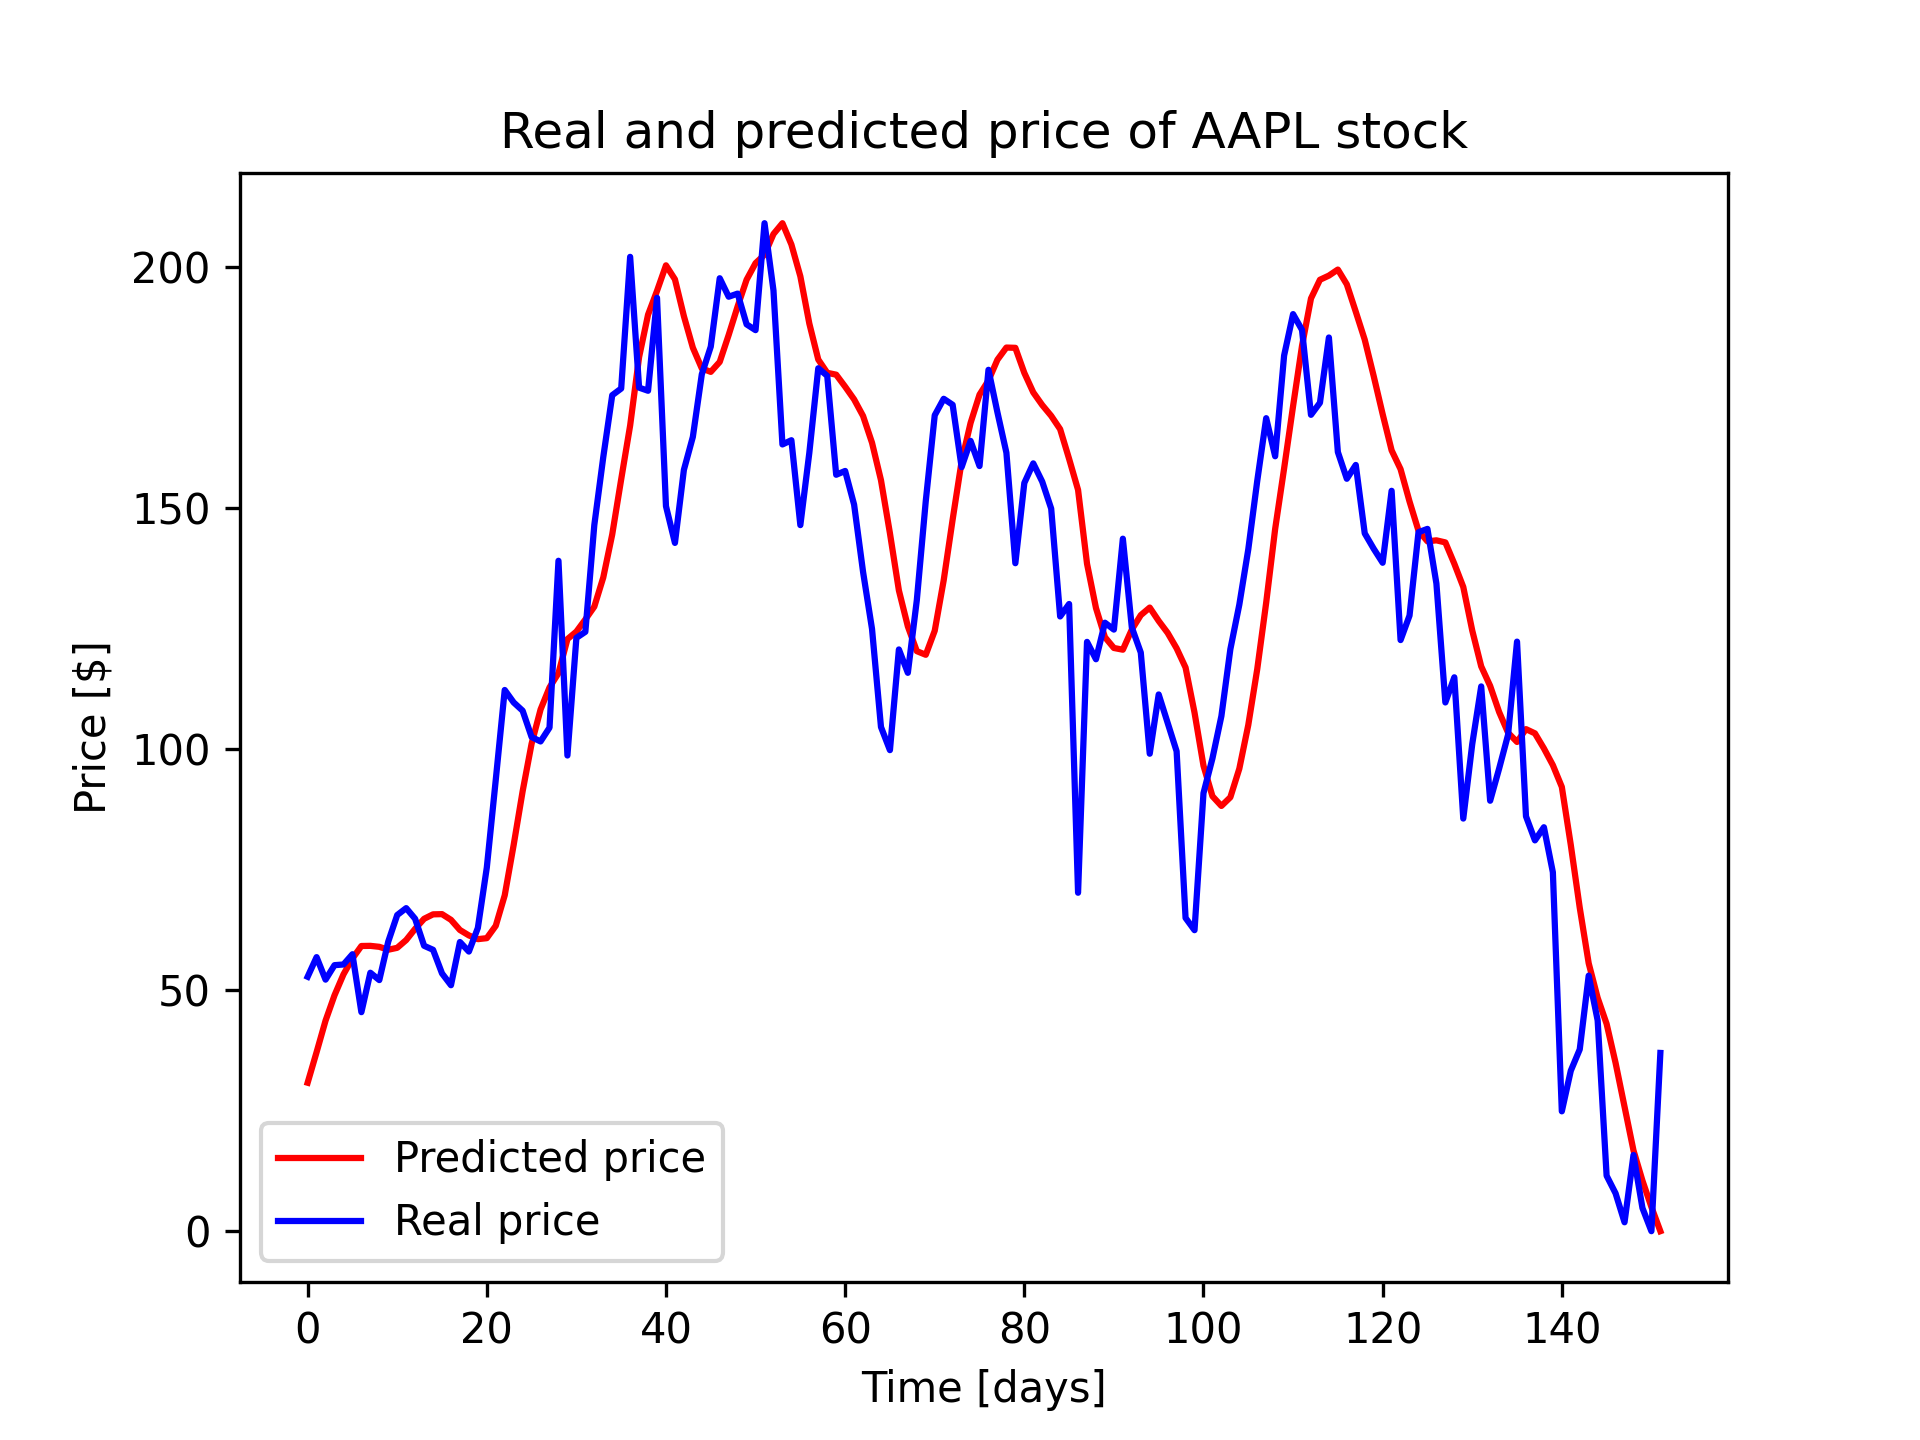
\includegraphics[width=0.5\textwidth]{./graf/model7/AAPL.png}
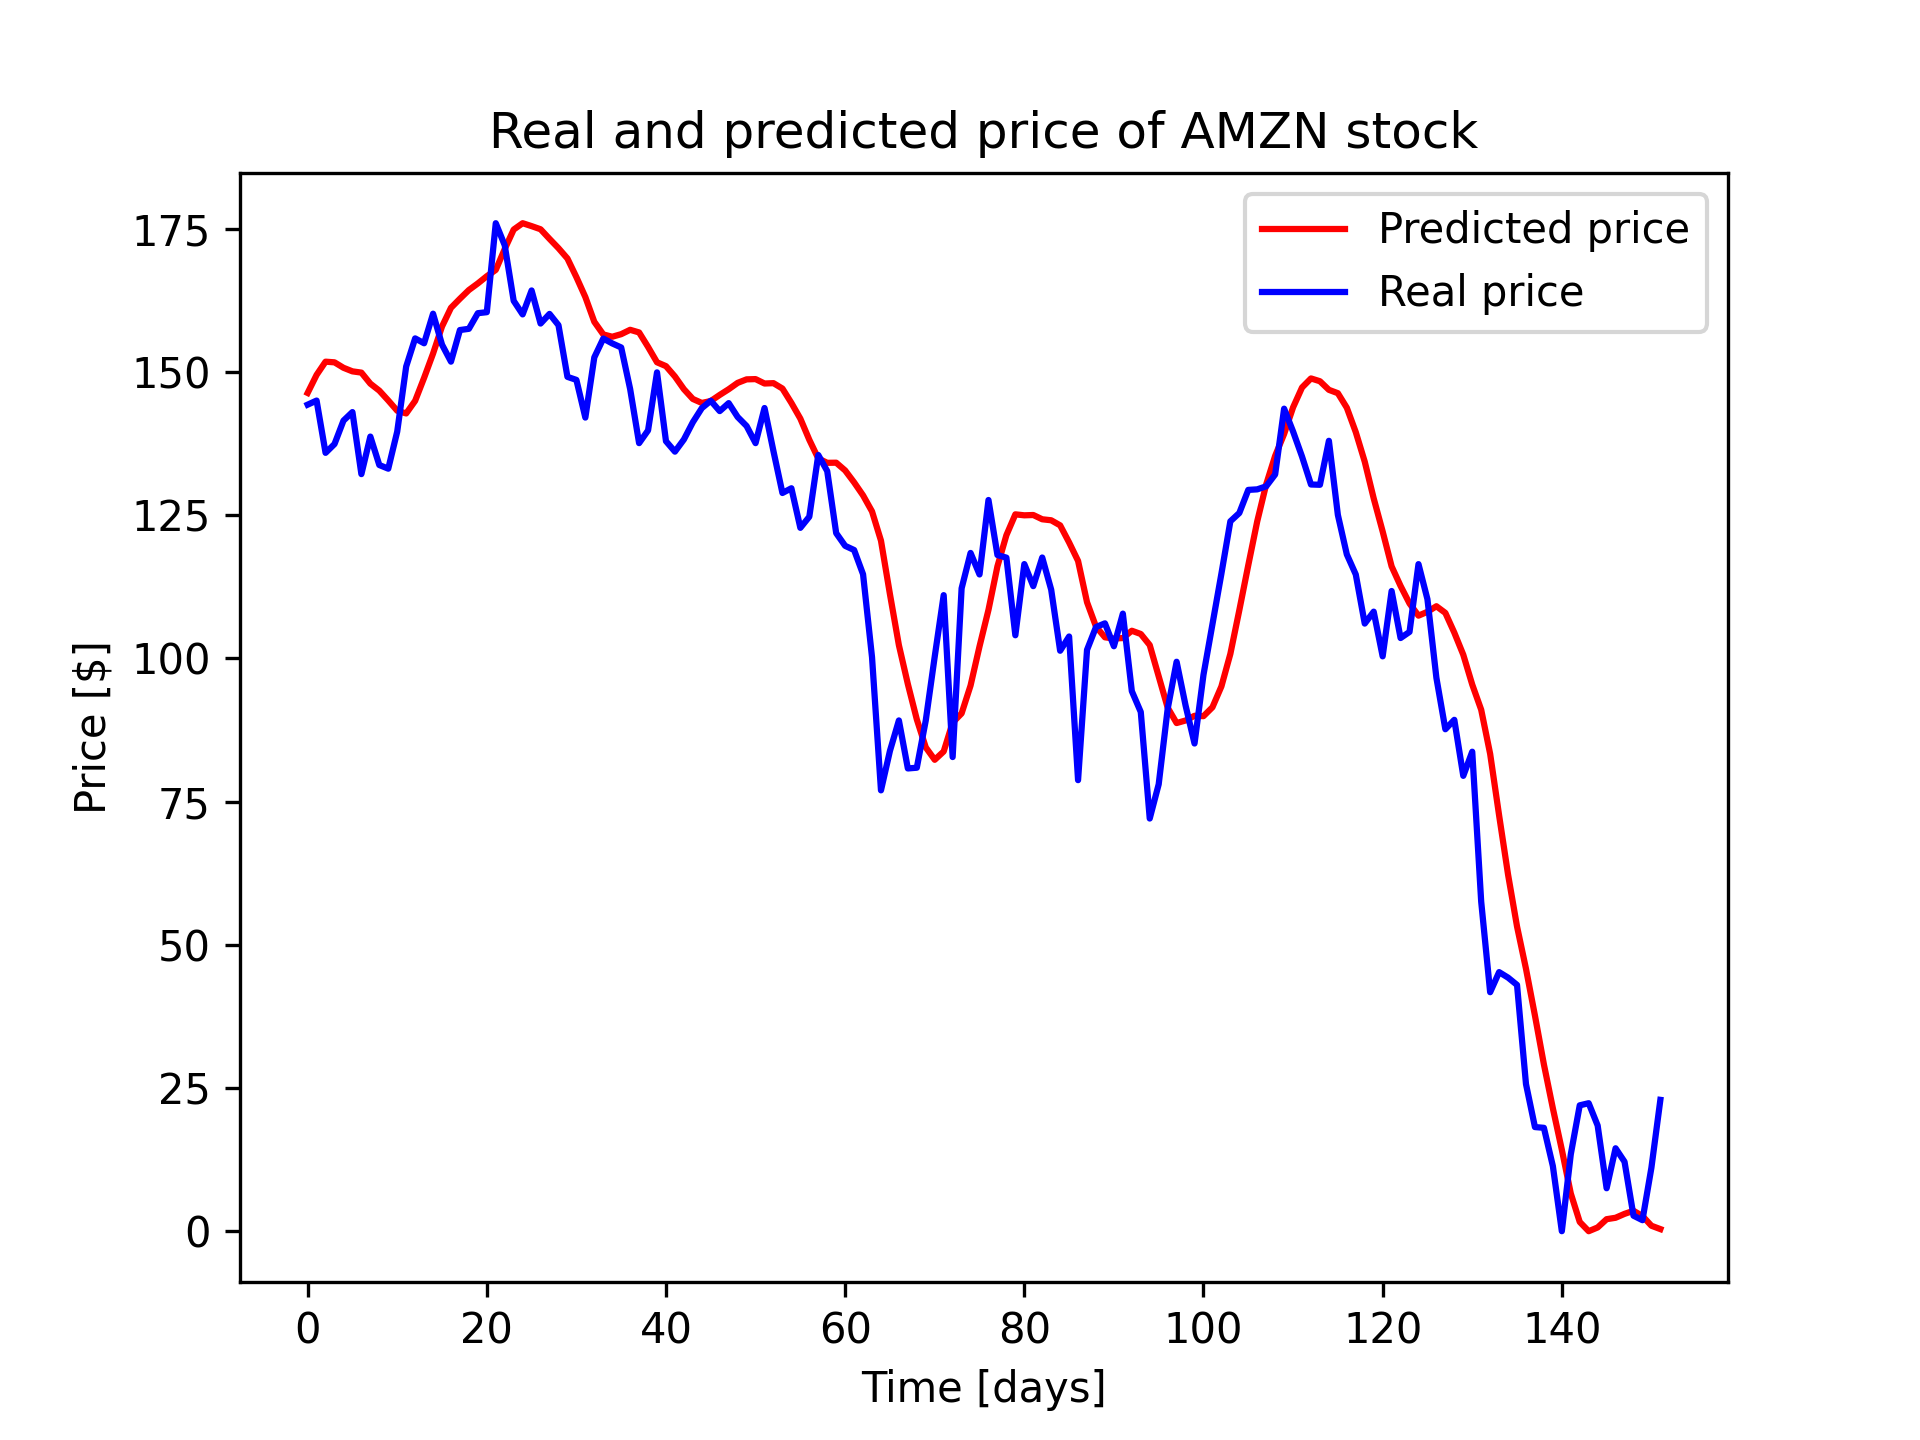
\includegraphics[width=0.5\textwidth]{./graf/model7/AMZN.png}
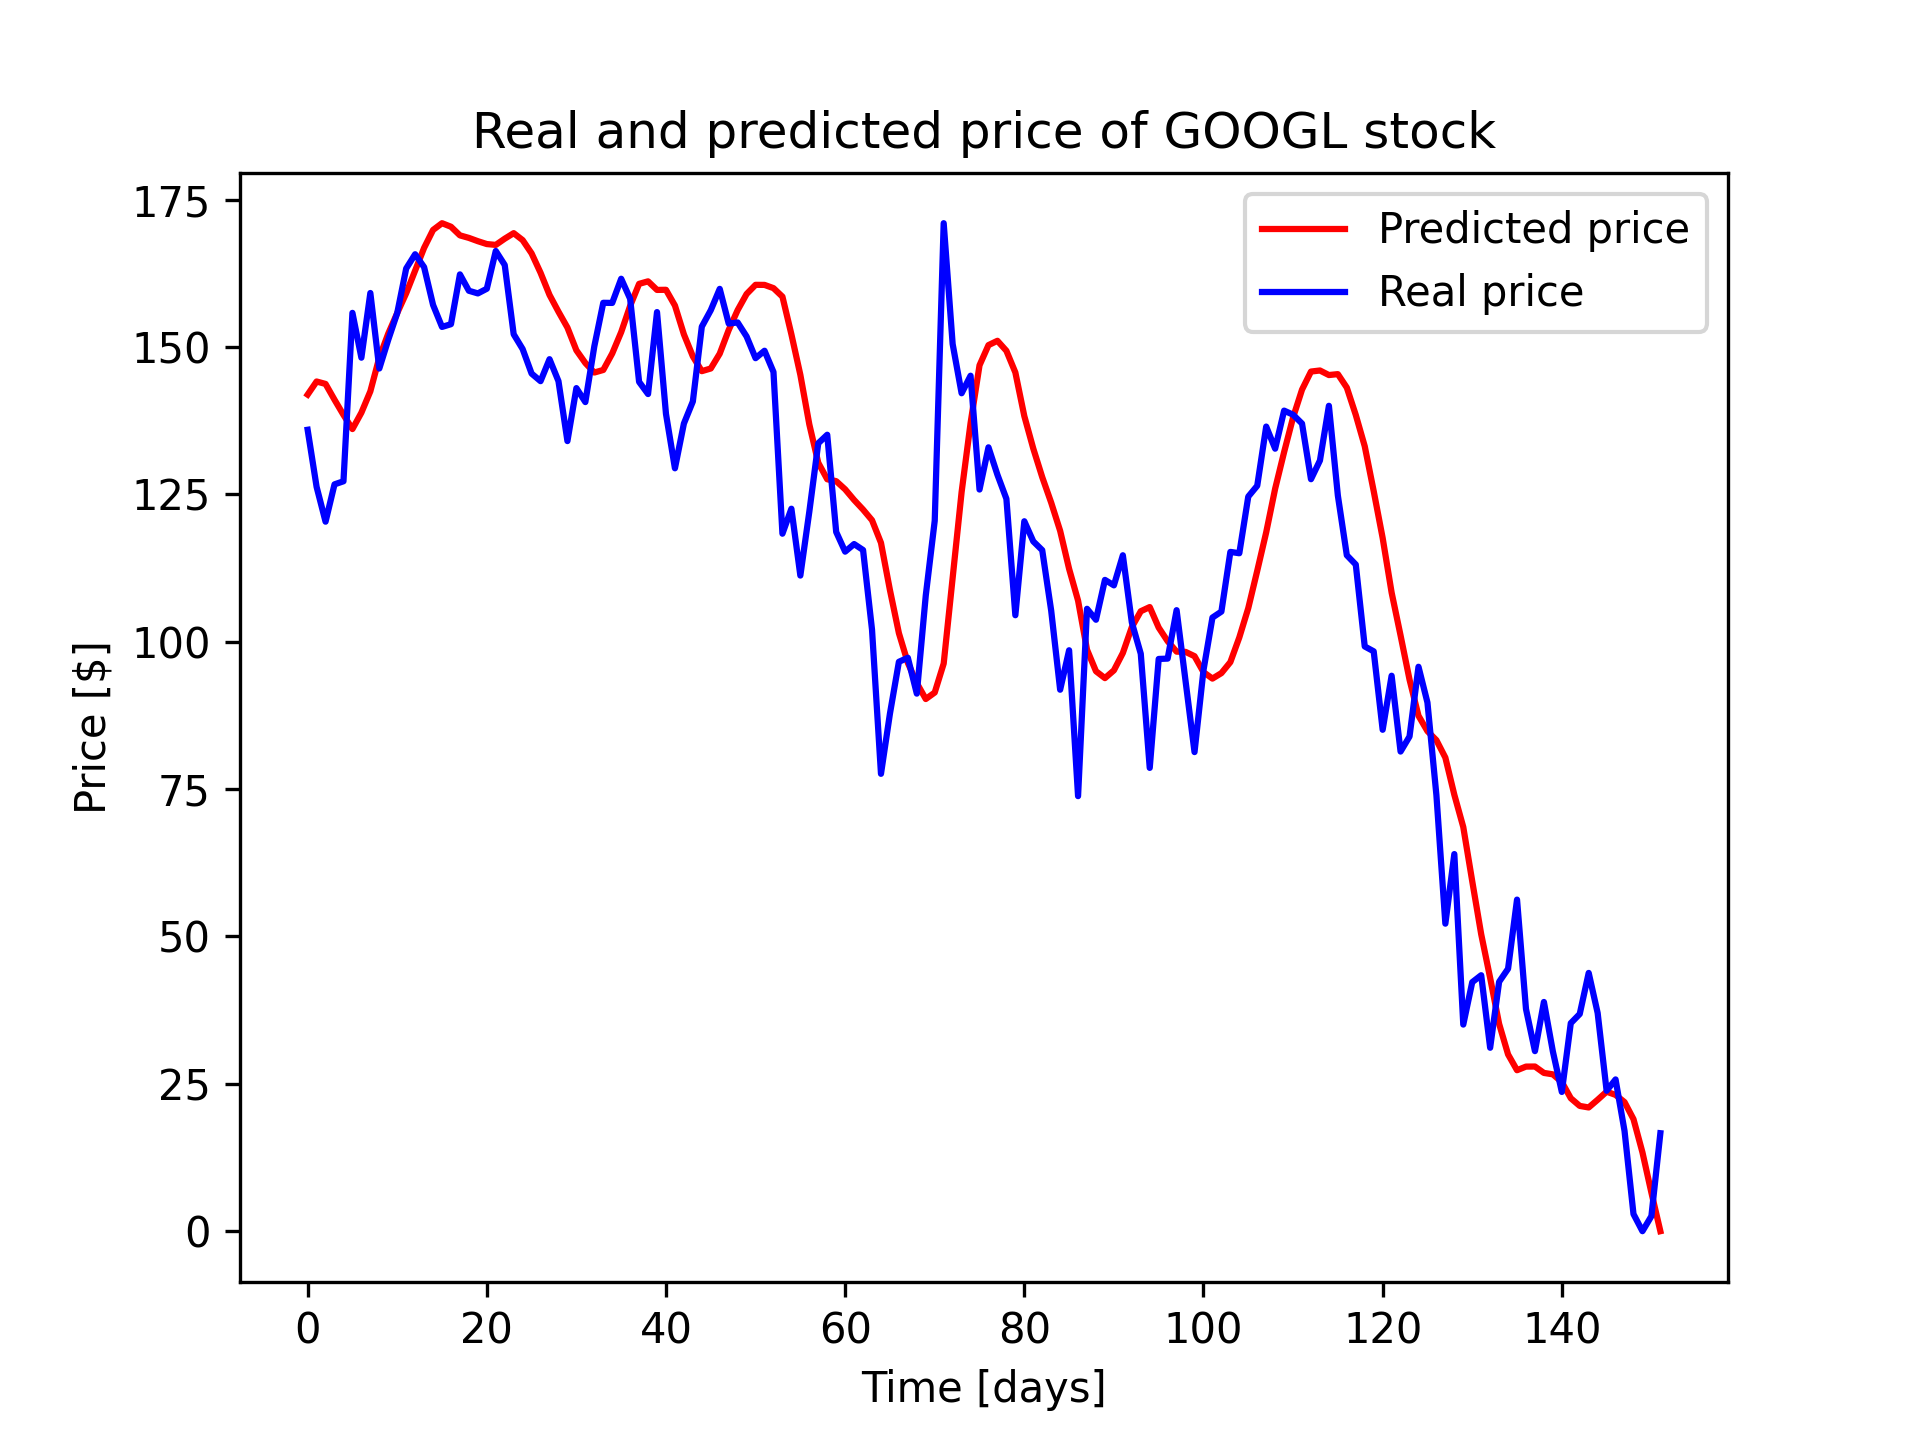
\includegraphics[width=0.5\textwidth]{./graf/model7/GOOGL.png}
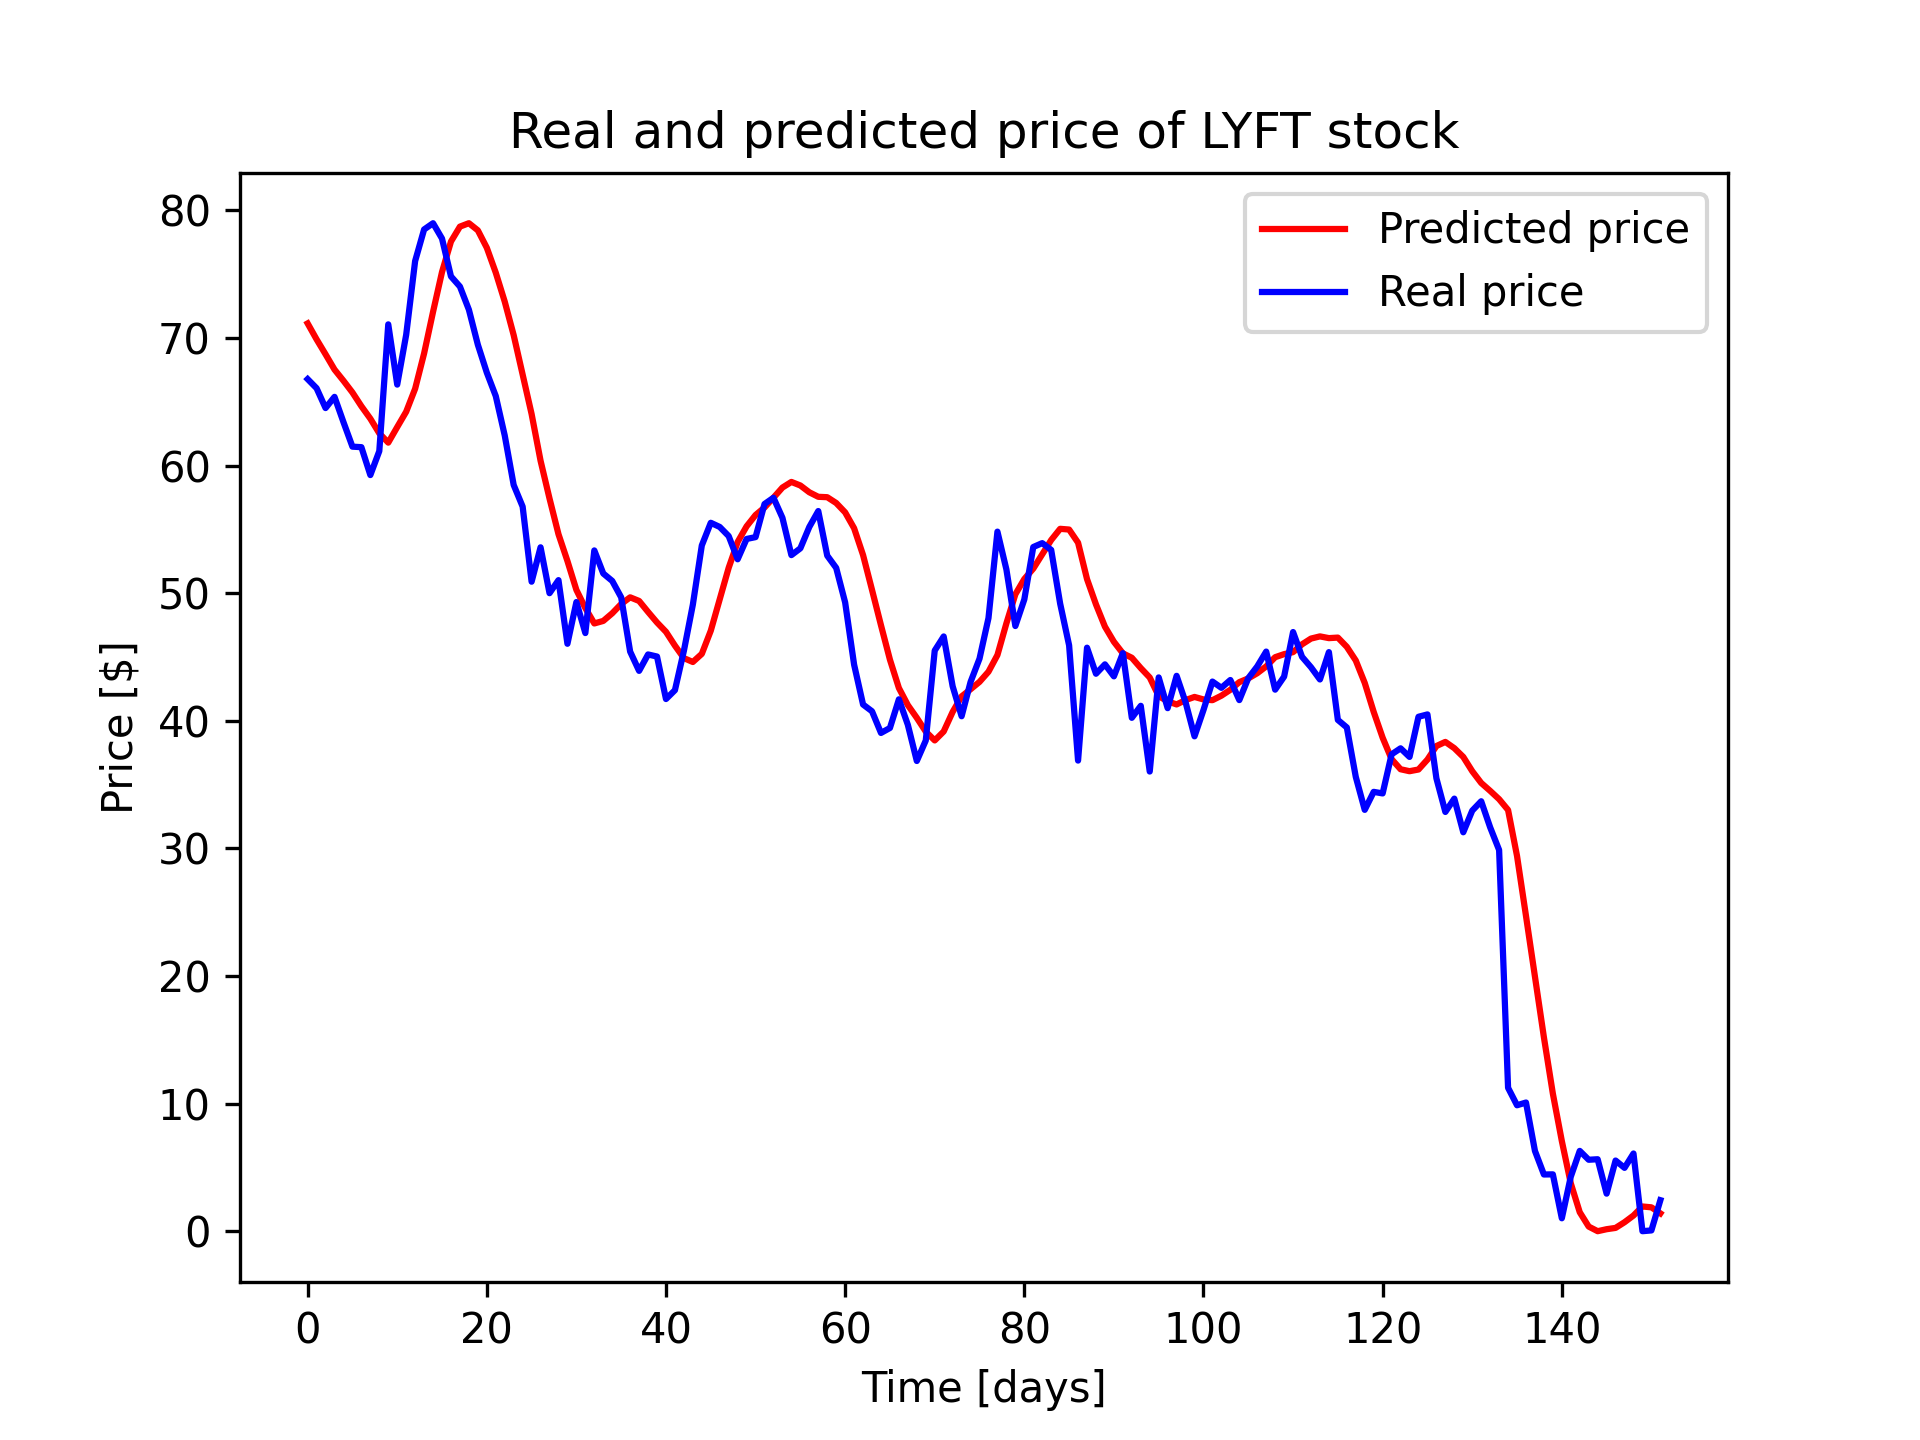
\includegraphics[width=0.5\textwidth]{./graf/model7/LYFT.png}
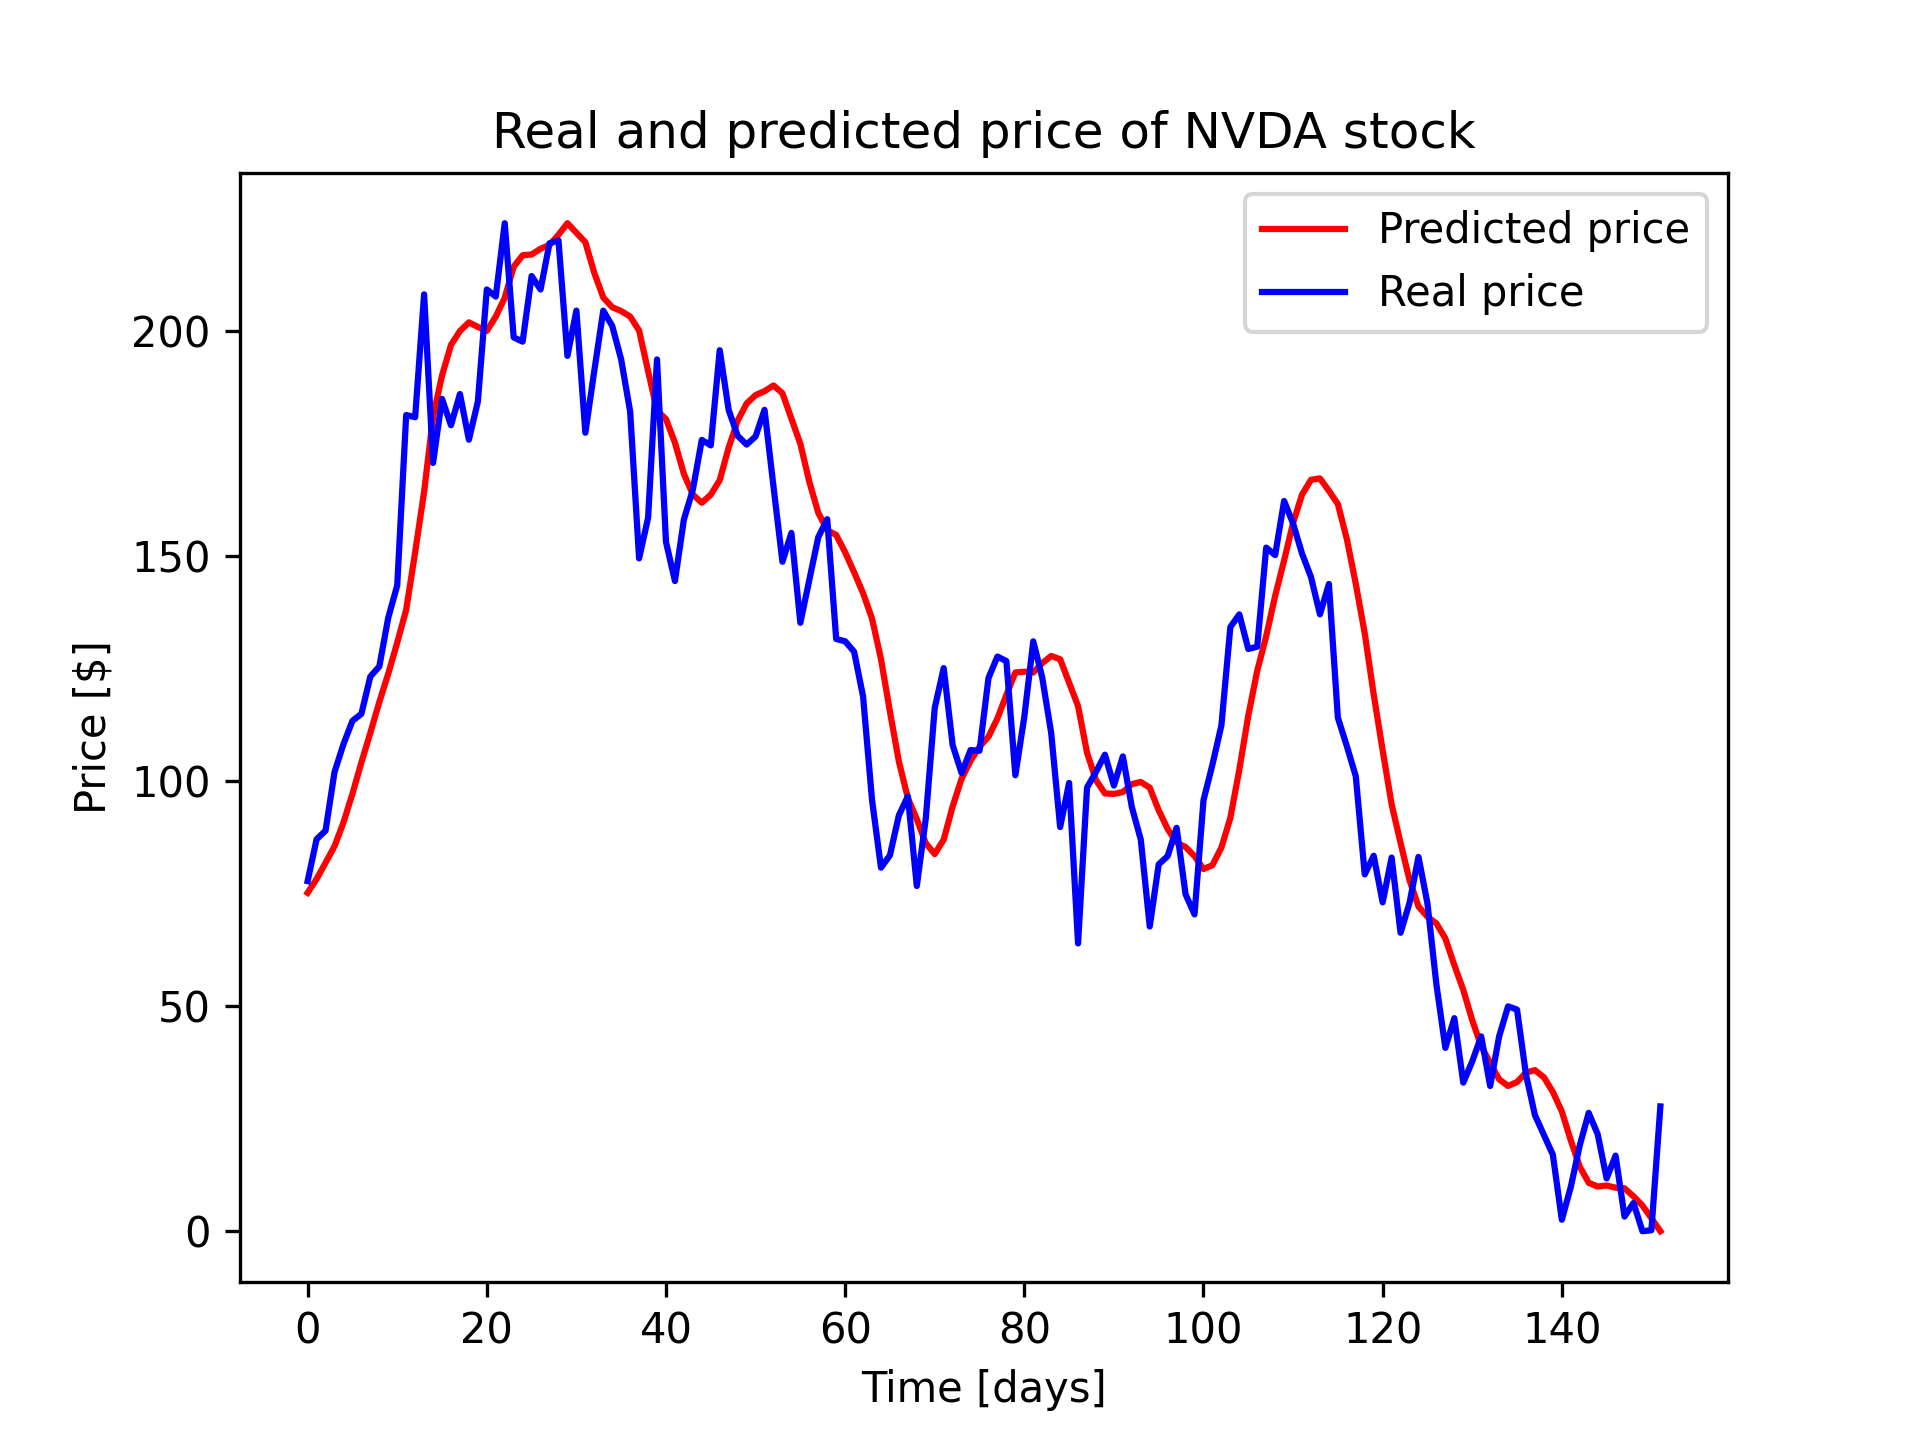
\includegraphics[width=0.5\textwidth]{./graf/model7/NVDA.png}
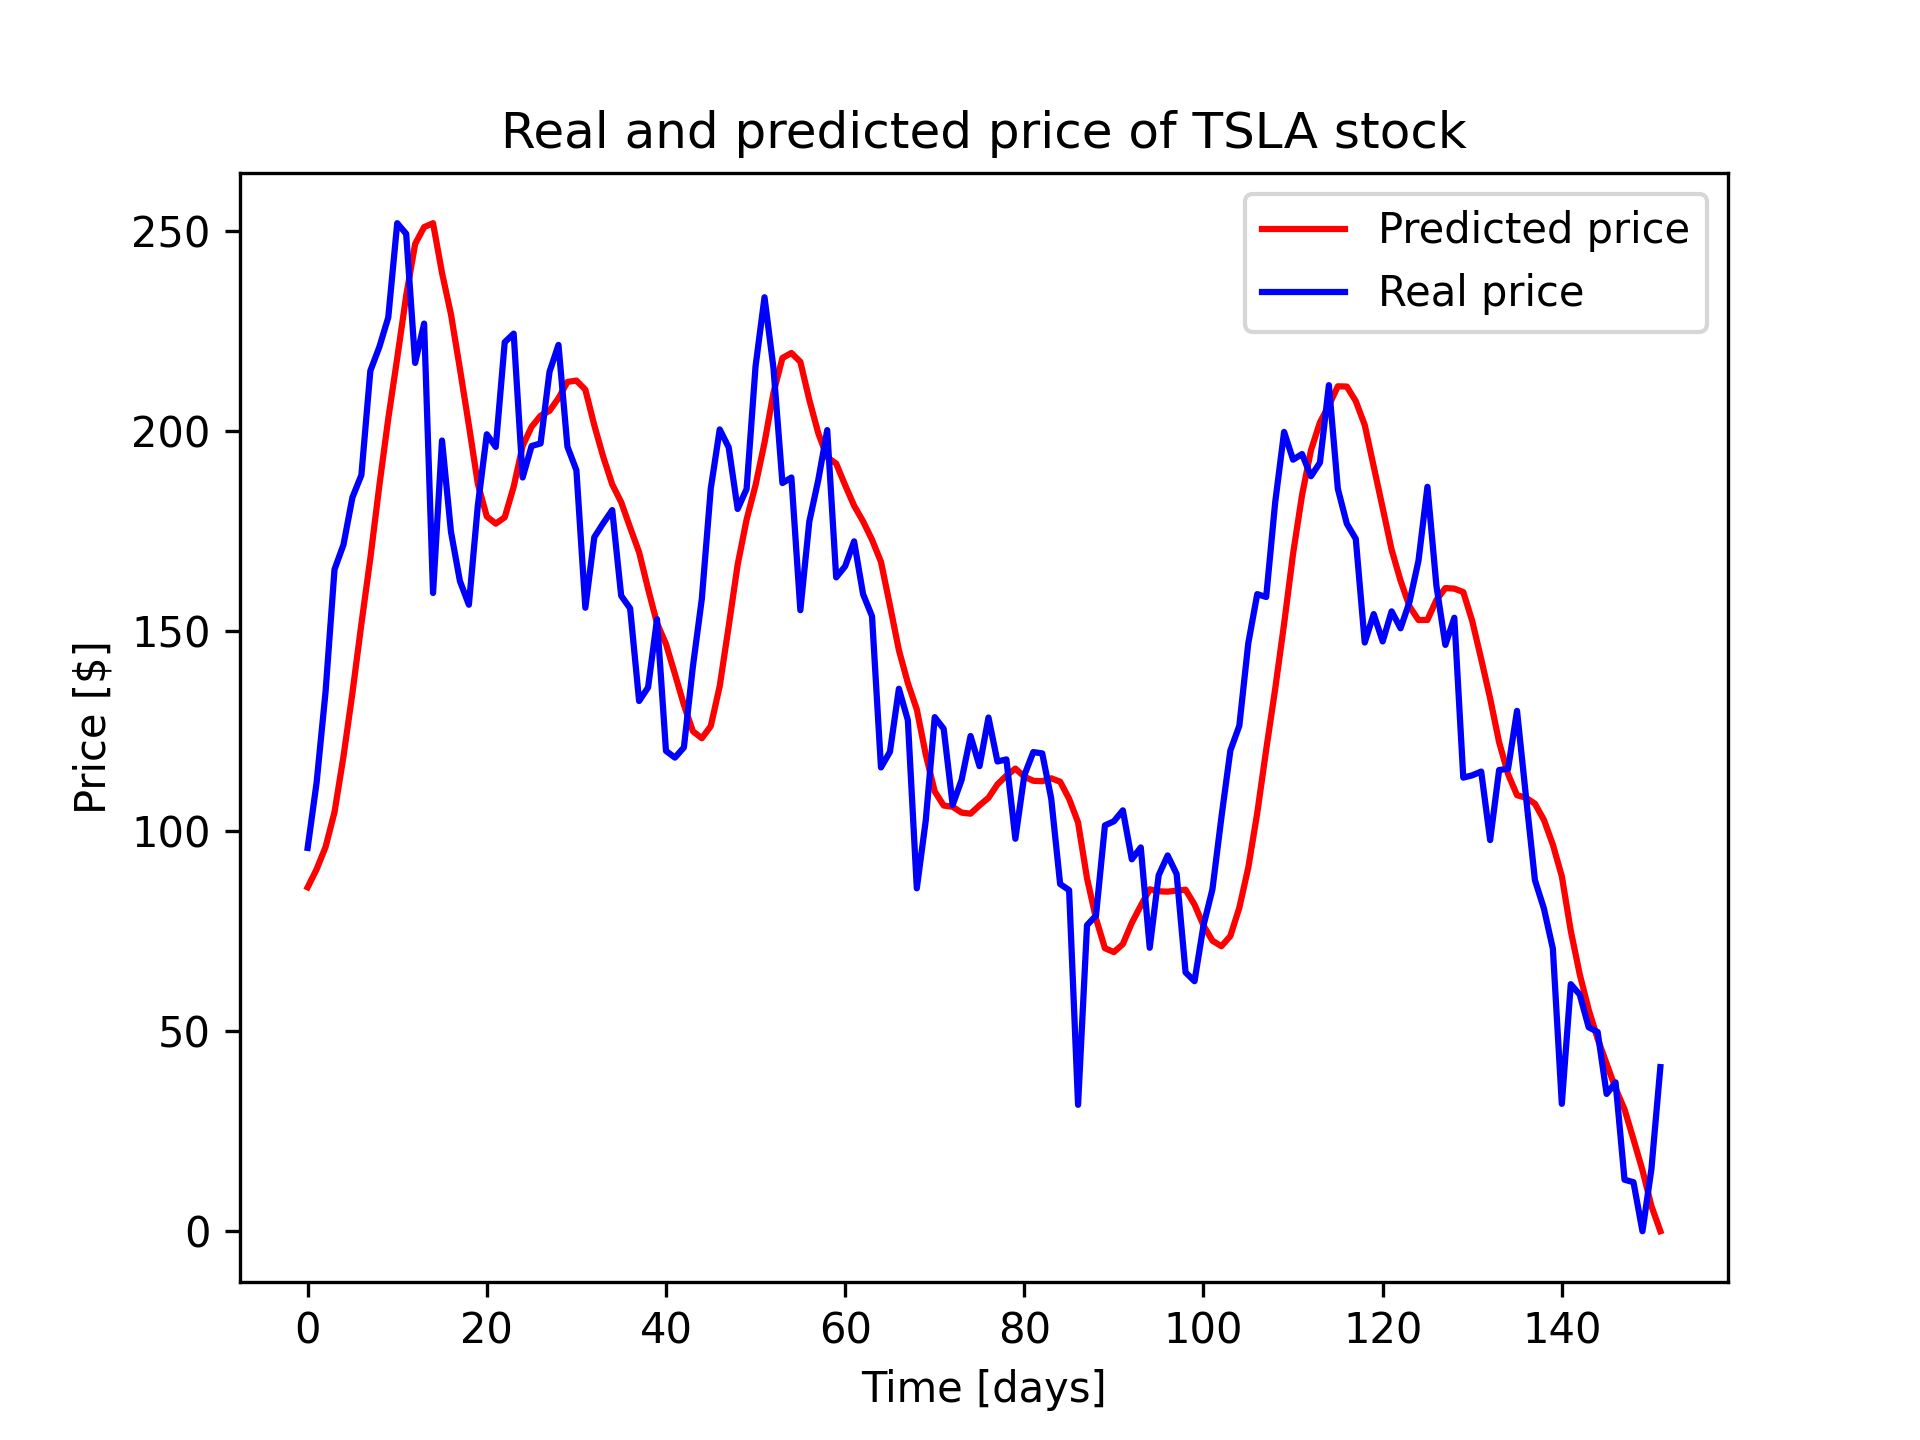
\includegraphics[width=0.5\textwidth]{./graf/model7/TSLA.png}
\caption{Real and predicted prices of the seventh model.}
\label{fig:label}
\end{figure} 

\clearpage
\subsection{Model 8}

Model8 - chunkSize: 100, time interval: 1 year, epochs: 10, trained on AAPL\par\bigskip
In the graphs of this model, one can observe the shift of the red line upwards relative to the blue line.
The general route of the two lines does not coincide, however, it reflects the general tendency to
increase or decrease prices. Rapid price drops are signaled by a blue line, for example, in the chart for AAPL.png.,
and GOOGL.png. they are not reflected in the course of the blue line. The same is true in two cases of
a sudden one-day price increase, as in the charts for GOOGL.png., and NVDA.png.,
however, in these cases, the blue line peaks do not go much above the red line. In addition, the red
line has a much more gentle course compared to the blue line, and it is flattened in places with very rapid price changes. What is worth noticing, the long-term systematic progression of
prices is precisely marked, and both lines have an almost identical course.
\par\bigskip
loss: 0.010029036551713943\par
RMSE for AAPL equals 12.851150959540742\par
RMSE for AMZN equals 7.454121214576205\par
RMSE for GOOGL equals 9.329325048731752\par
RMSE for LYFT equals 2.8188979984881253\par
RMSE for NVDA equals 10.223120885378568\par
RMSE for TSLA equals 7.377703064209013\par

\begin{figure}
% \centering
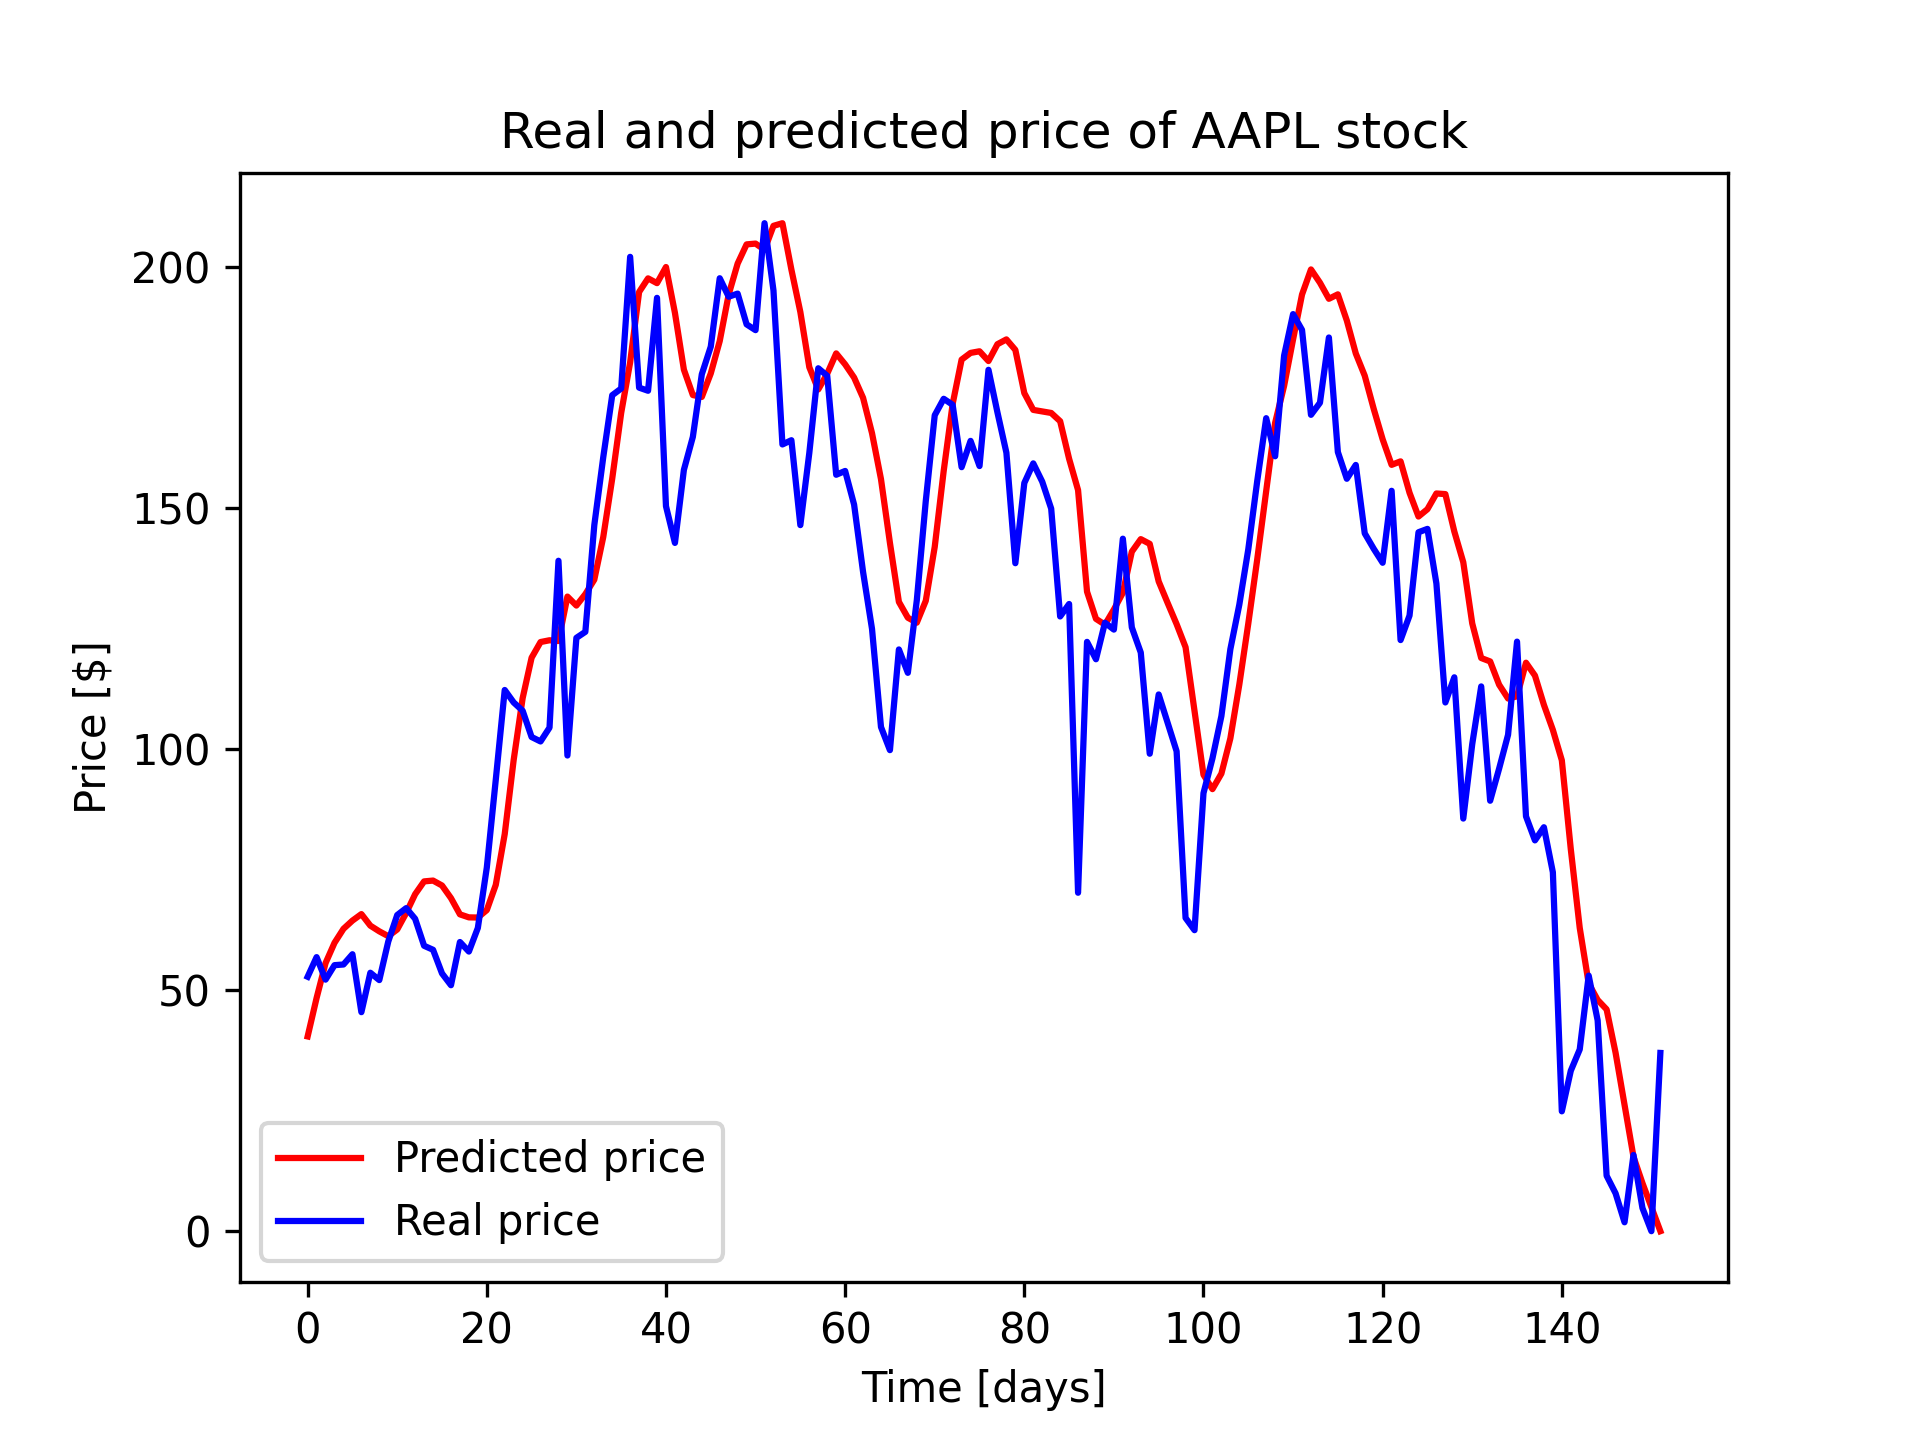
\includegraphics[width=0.5\textwidth]{./graf/model8/AAPL.png}
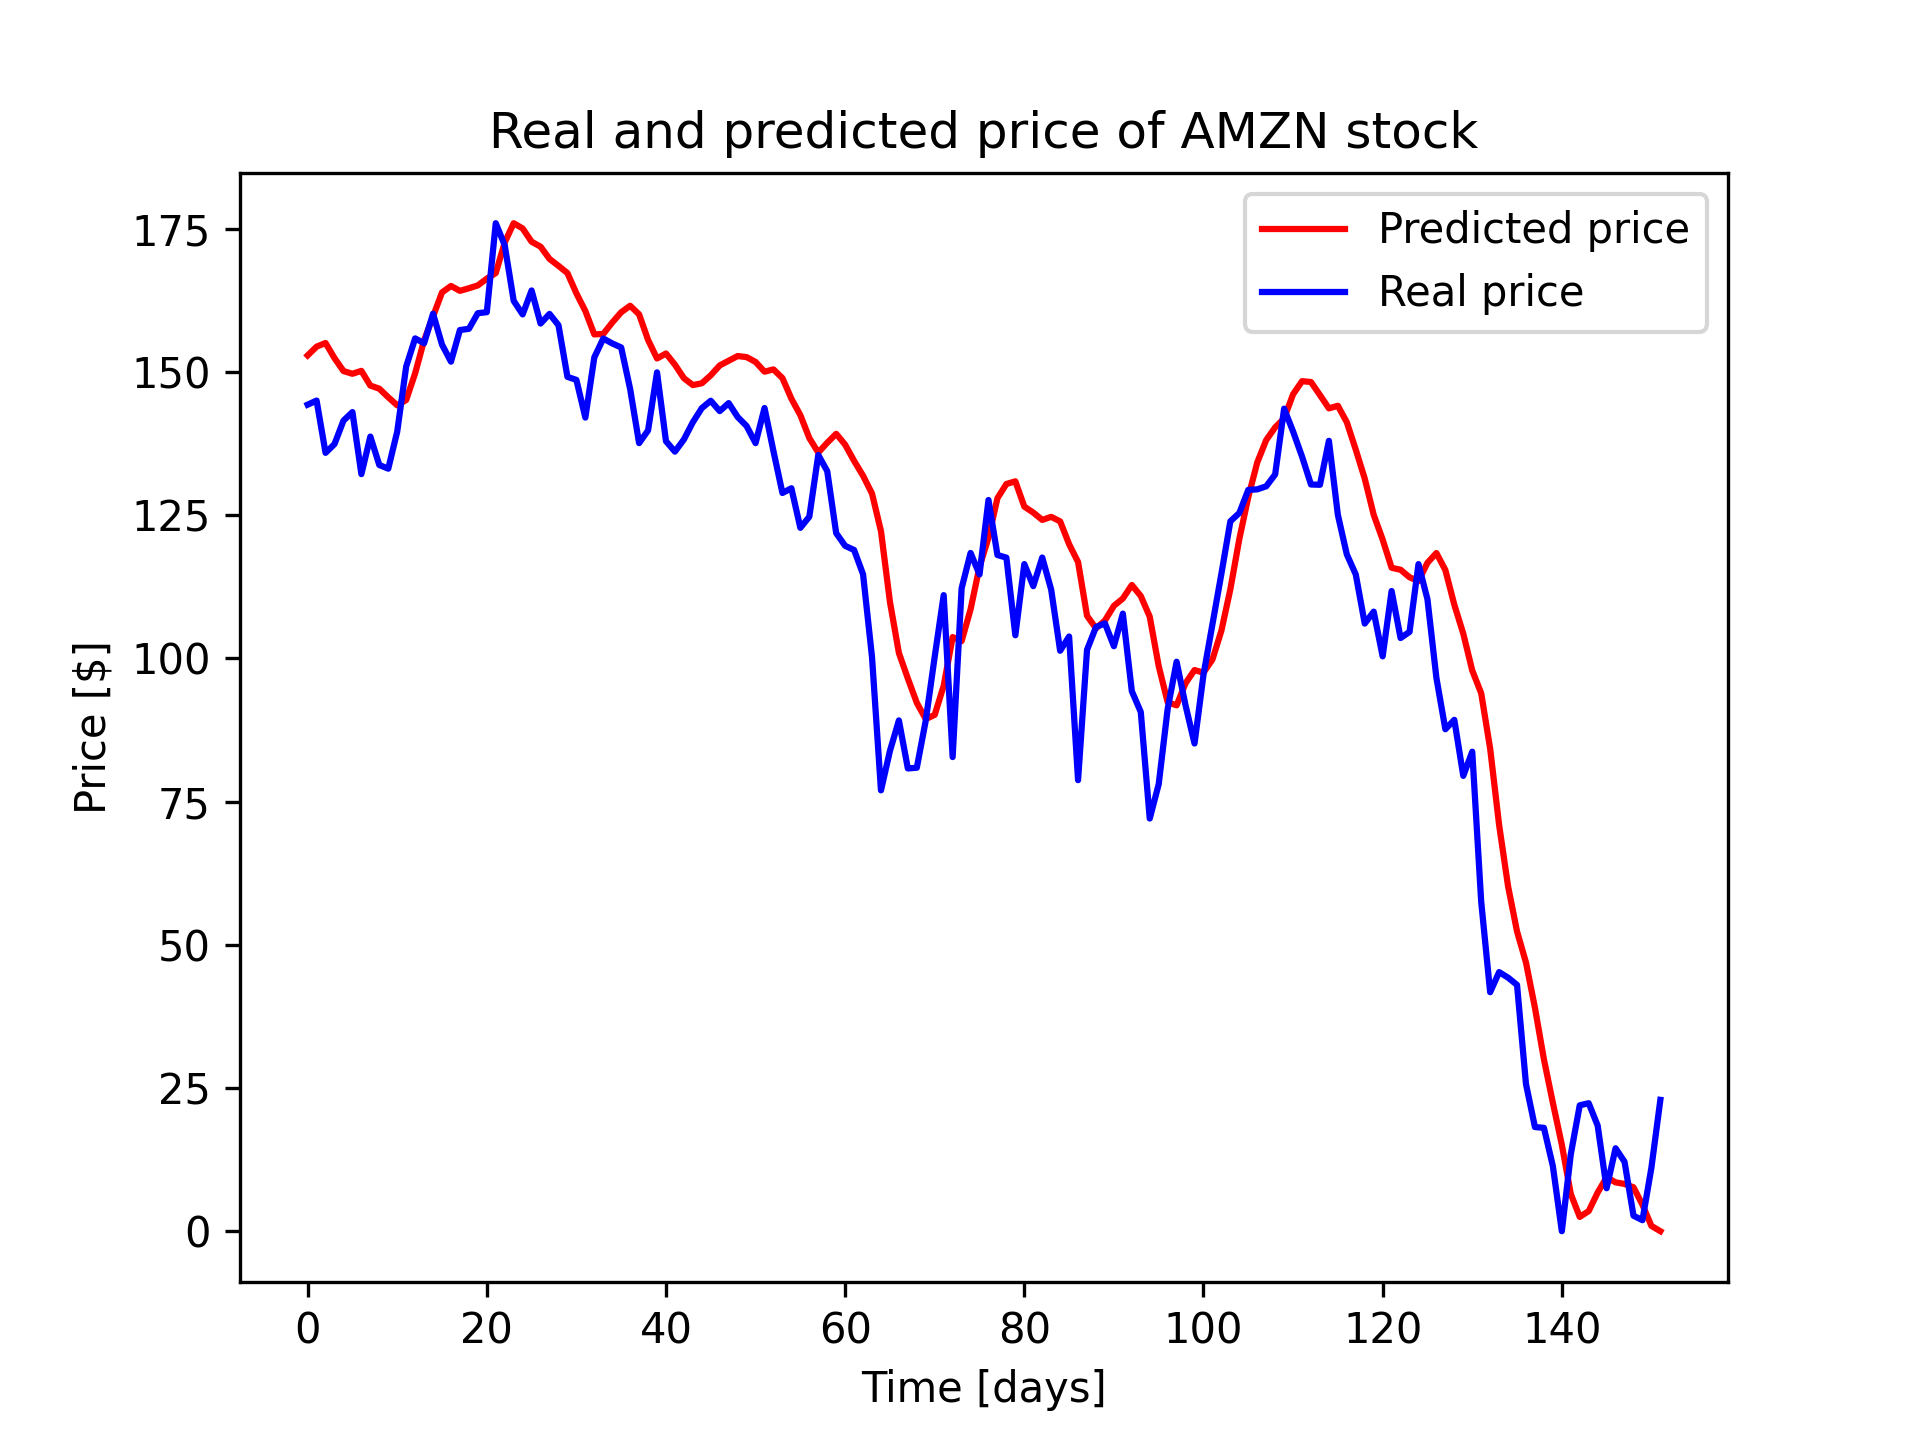
\includegraphics[width=0.5\textwidth]{./graf/model8/AMZN.png}
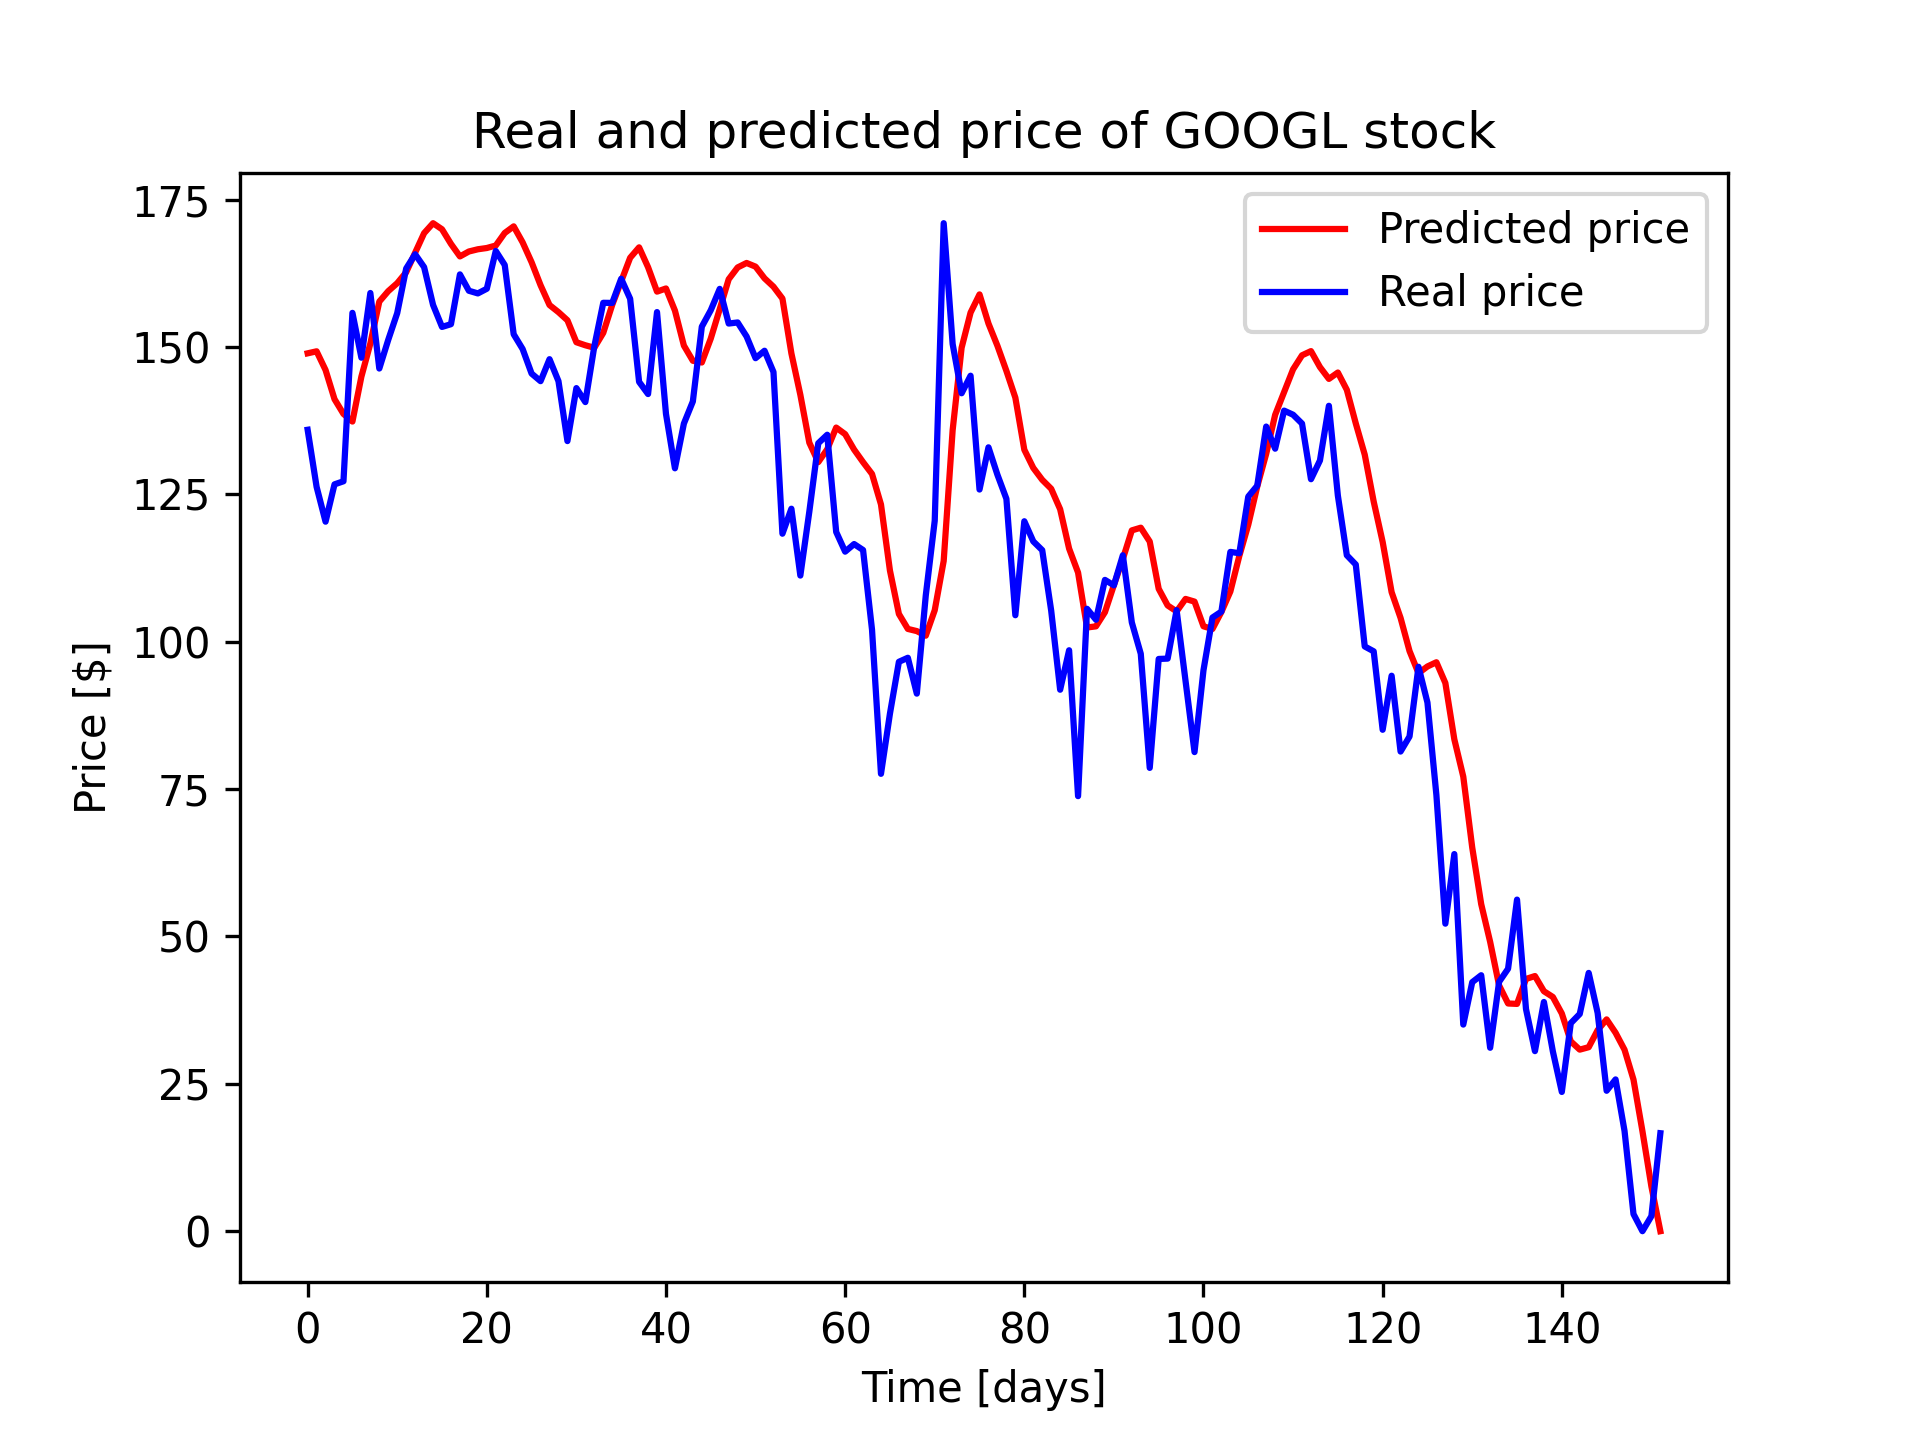
\includegraphics[width=0.5\textwidth]{./graf/model8/GOOGL.png}
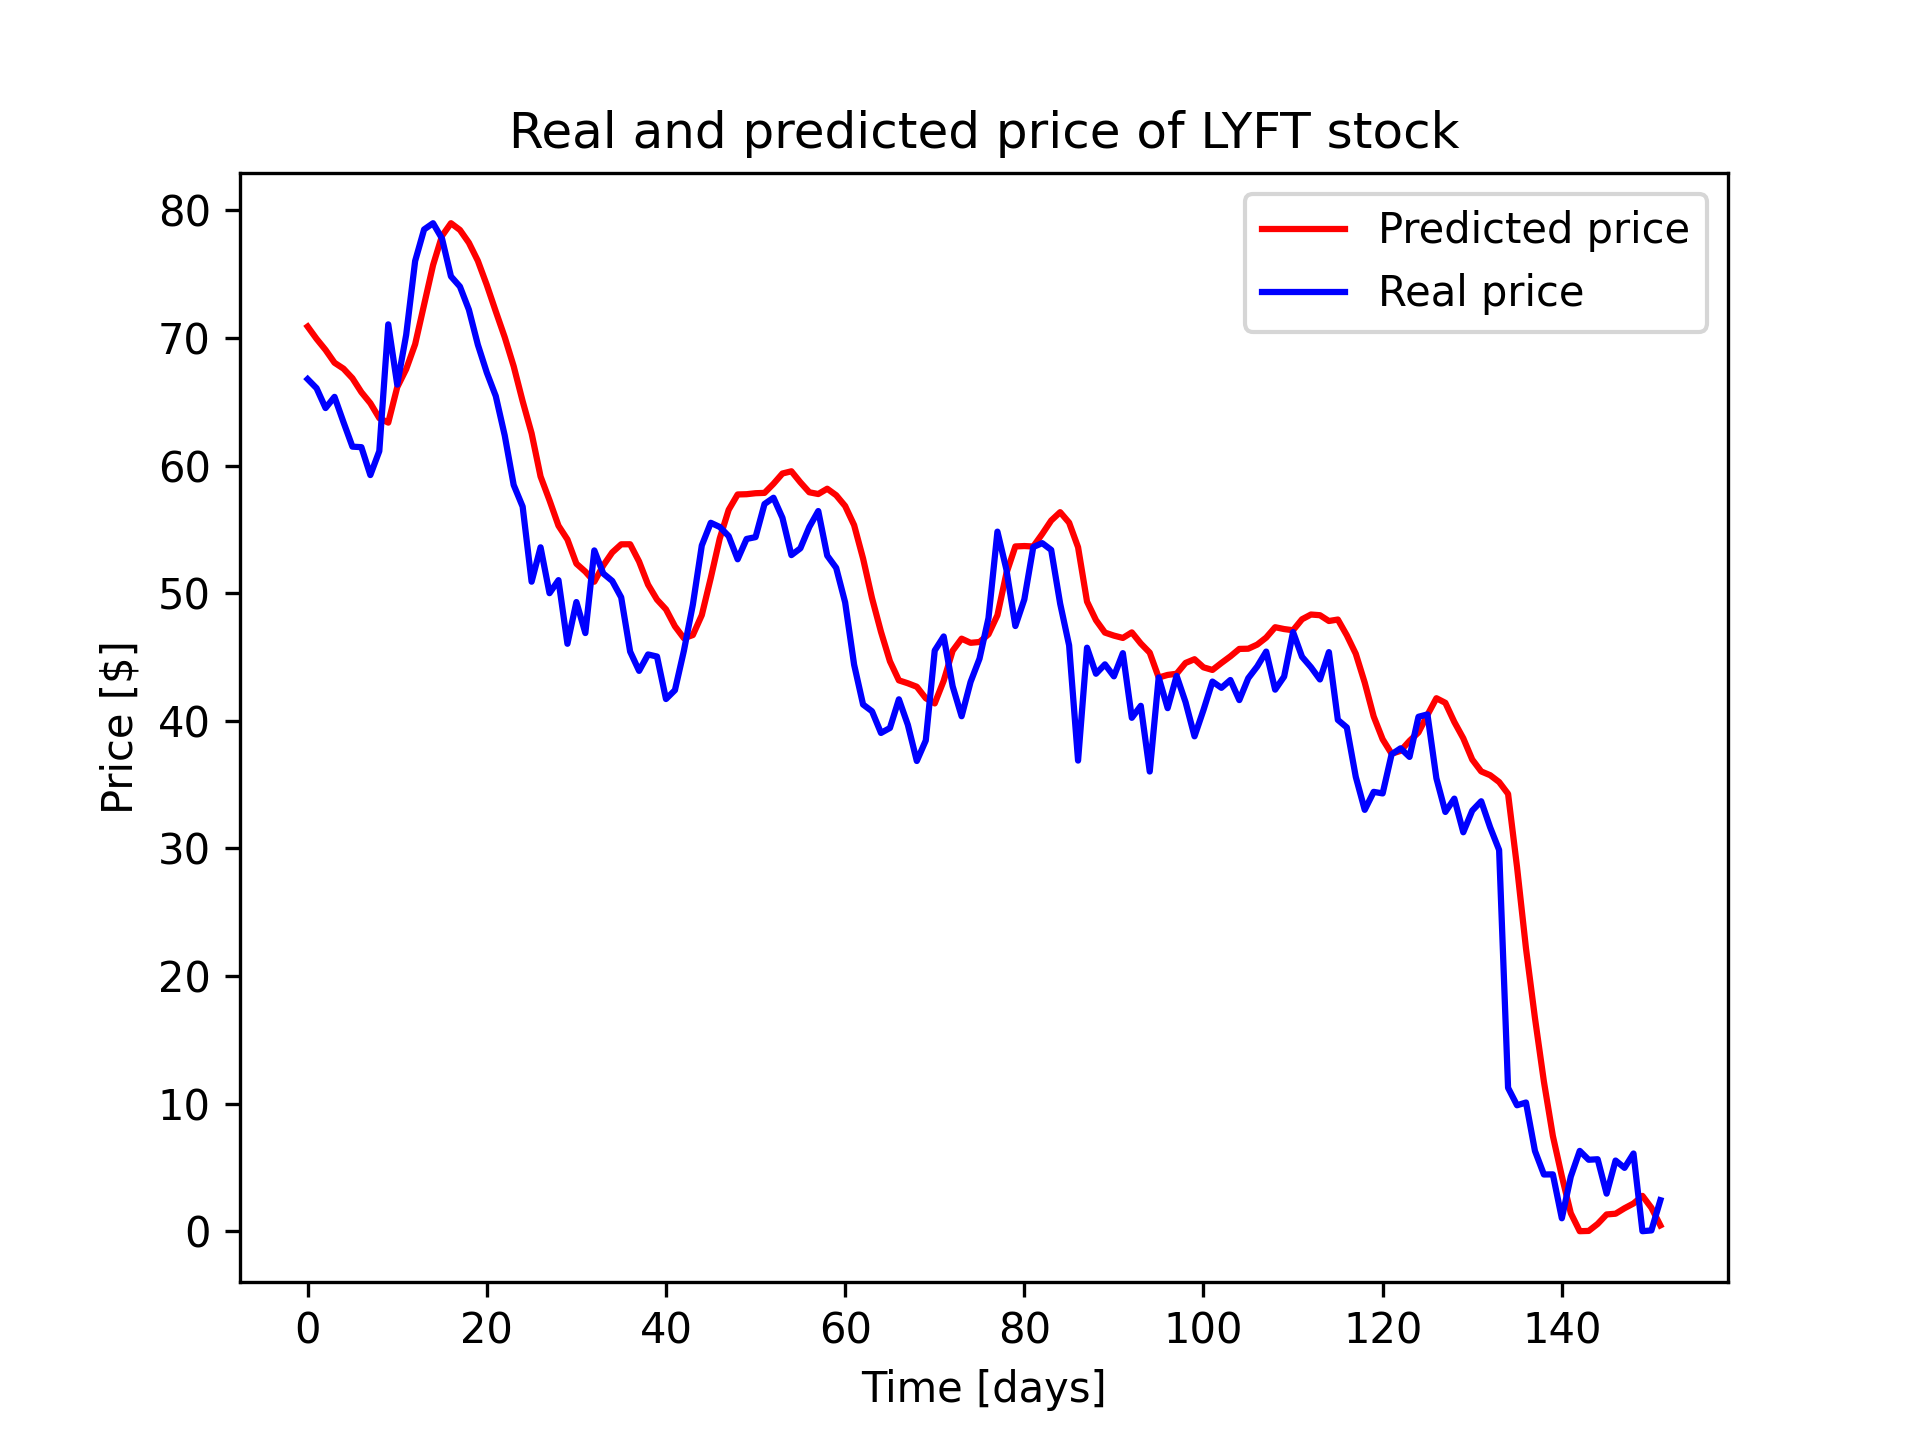
\includegraphics[width=0.5\textwidth]{./graf/model8/LYFT.png}
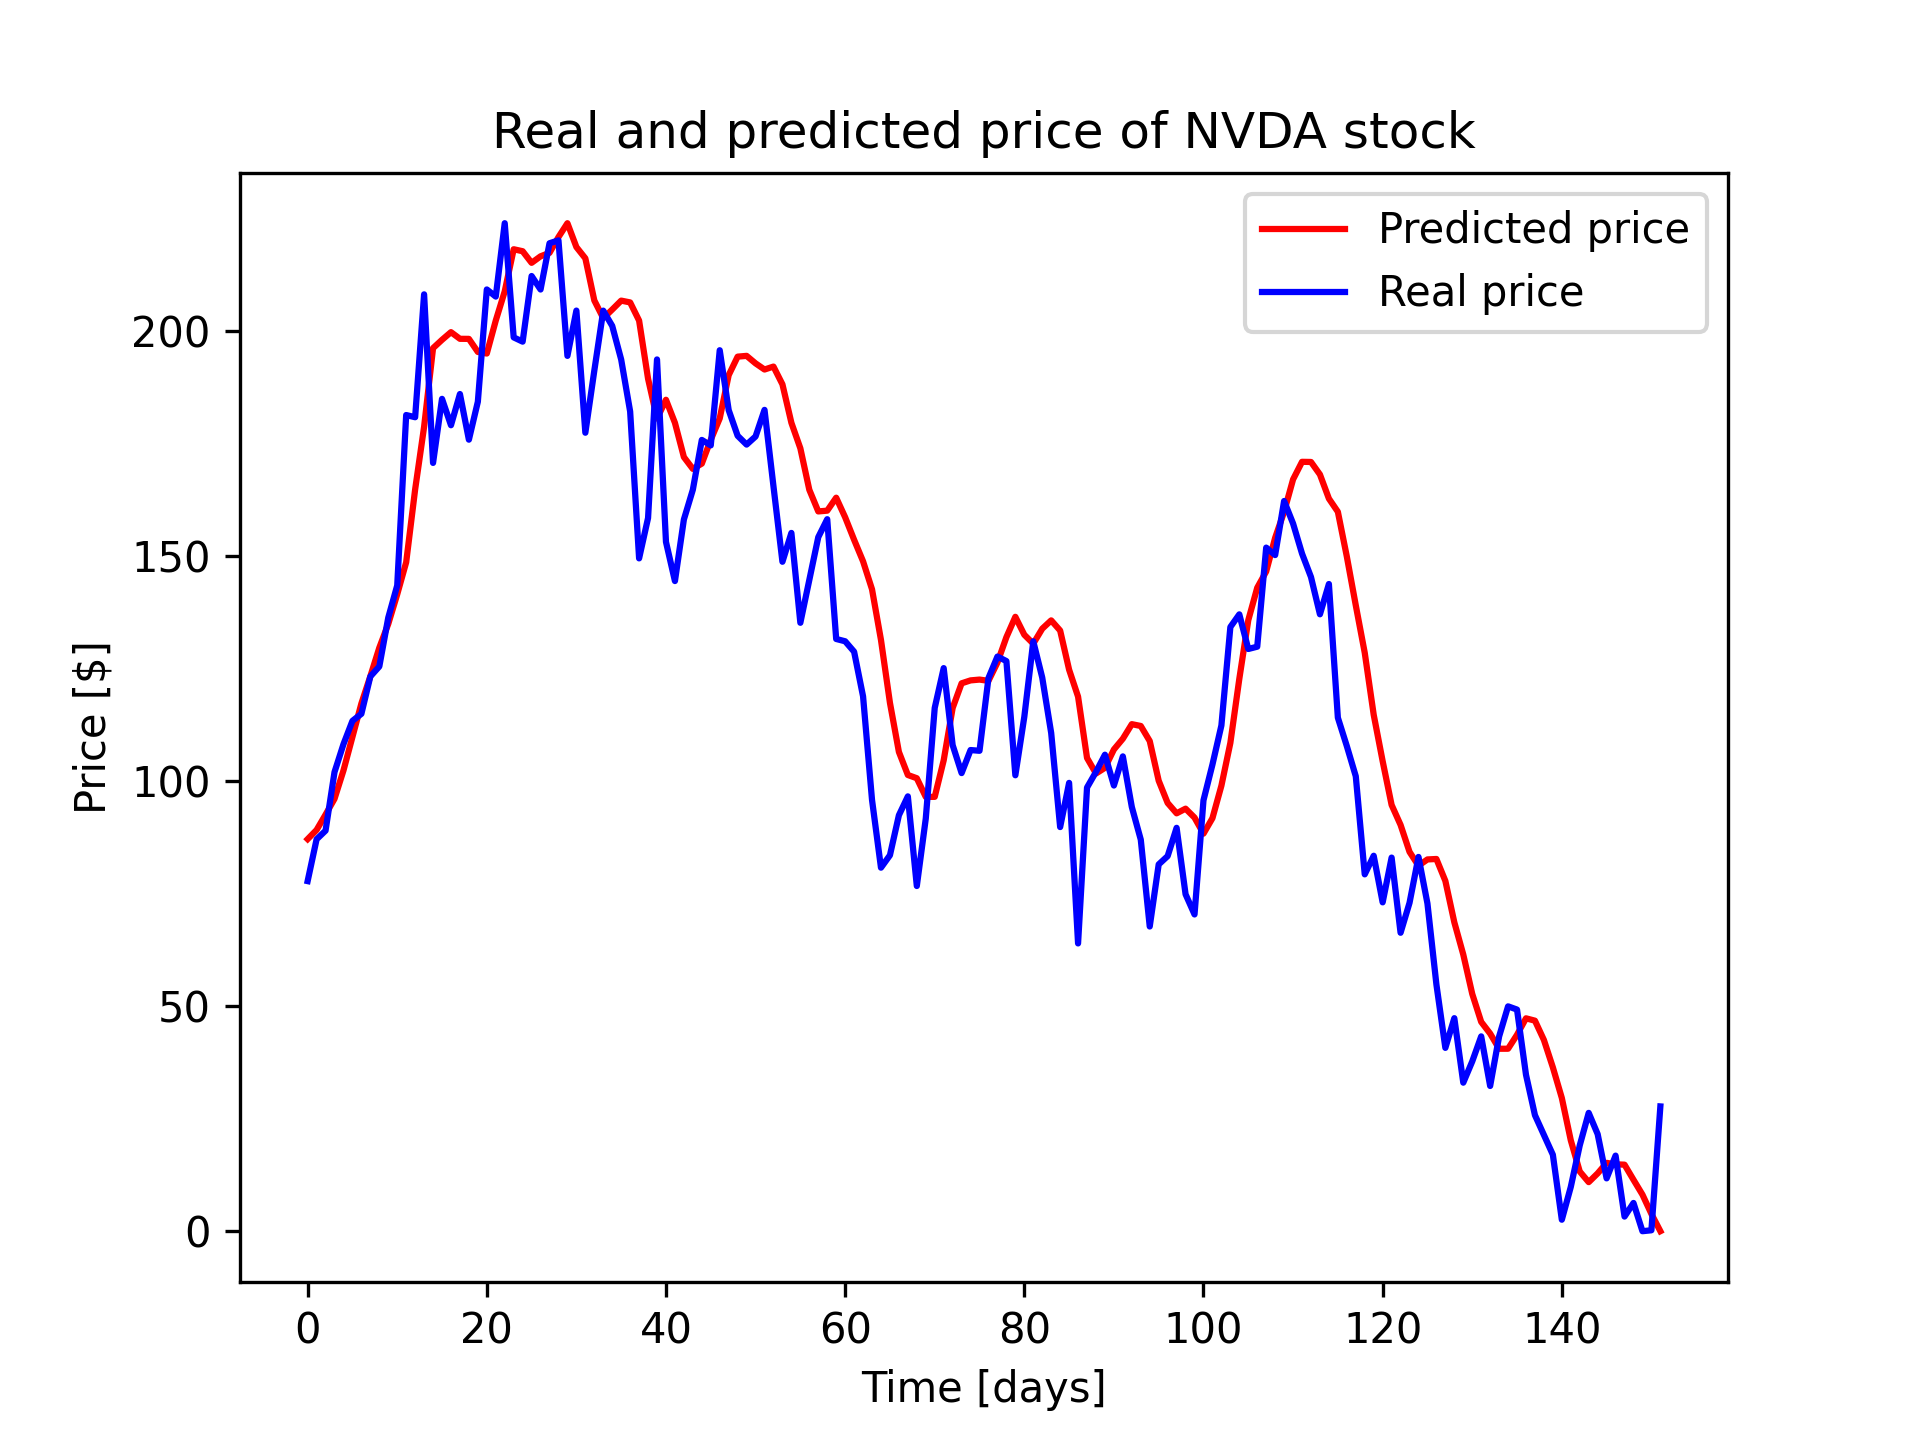
\includegraphics[width=0.5\textwidth]{./graf/model8/NVDA.png}
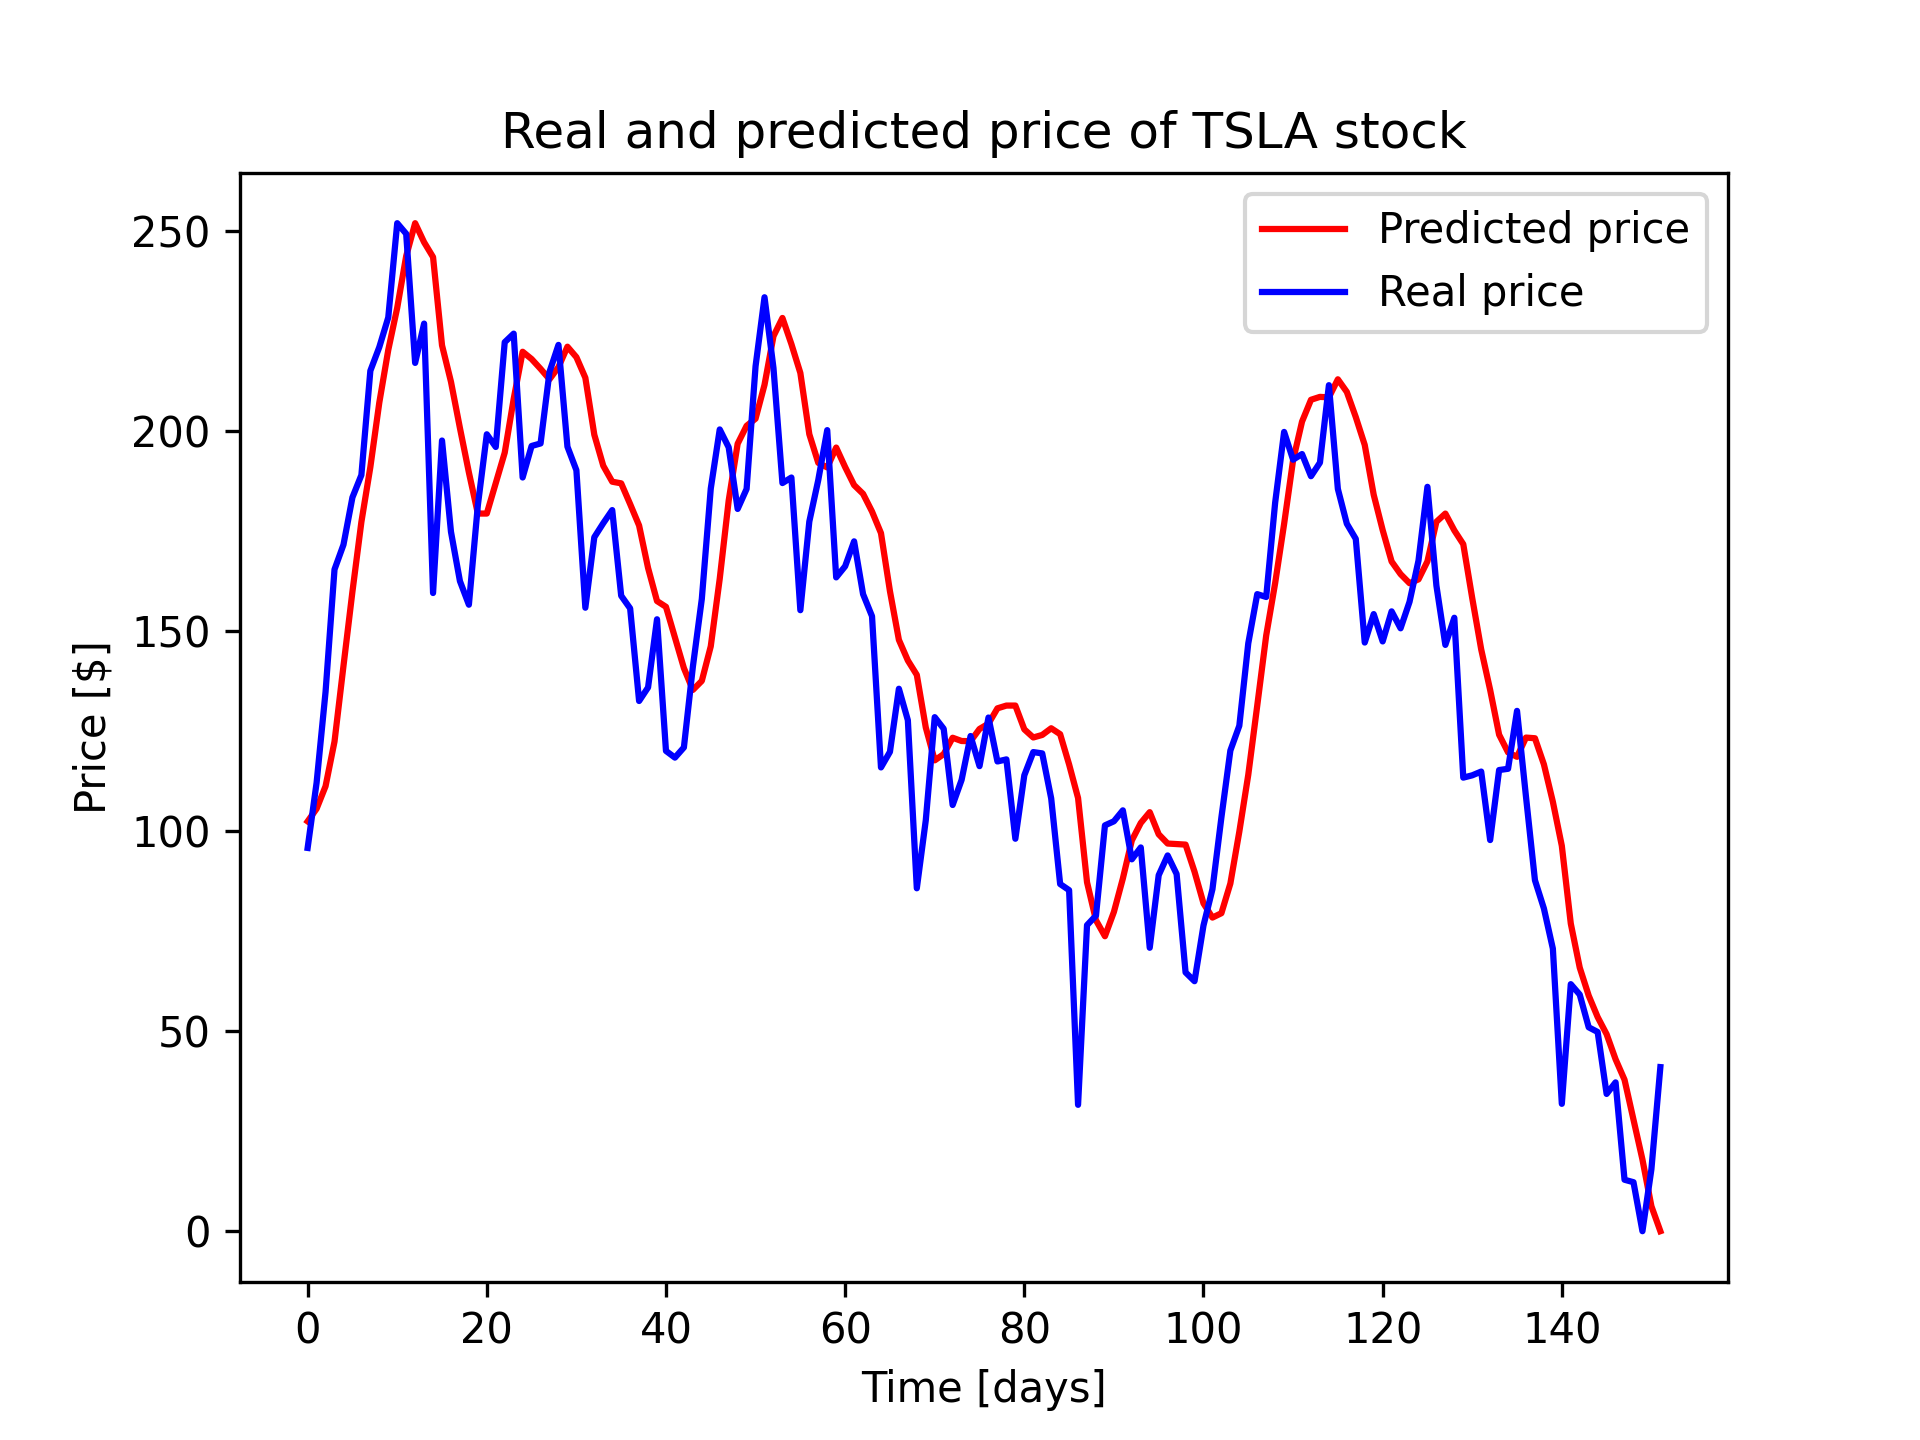
\includegraphics[width=0.5\textwidth]{./graf/model8/TSLA.png}
\caption{Real and predicted prices of the eighth model.}
\label{fig:label}
\end{figure} 

\clearpage
\subsection{Model 9}

Model9 - chunkSize: 100, time interval: 1 year, epochs: 15, trained on AAPL\par\bigskip
In this model, both lines have a very similar course in terms of deflection up or to the side. The lines
in the aged places of the charts coincide with each other. One can also see places on the charts
where the lines intersect, but the general trend in the course of the lines shows a consistent picture
of predicting market prices. The longer-lasting, consistent increase in market prices is very well
illustrated in the chart for NVDA.png., GOOGL.png, AAPL.png, and TSLA.png. On the other hand,
sharp one-day price drops reflected in sharply deflected down peaks, for example, TSLA.png or AAPL.png
do not translate into the course of the blue line.
\par\bigskip
loss: 0.007714248728007078\par
RMSE for AAPL equals 11.88924944538701\par
RMSE for AMZN equals 5.480018686104509\par
RMSE for GOOGL equals 8.8859280161446\par
RMSE for LYFT equals 2.099414458241764\par
RMSE for NVDA equals 8.83767288601412\par
RMSE for TSLA equals 5.368450472072029\par

\begin{figure}
% \centering
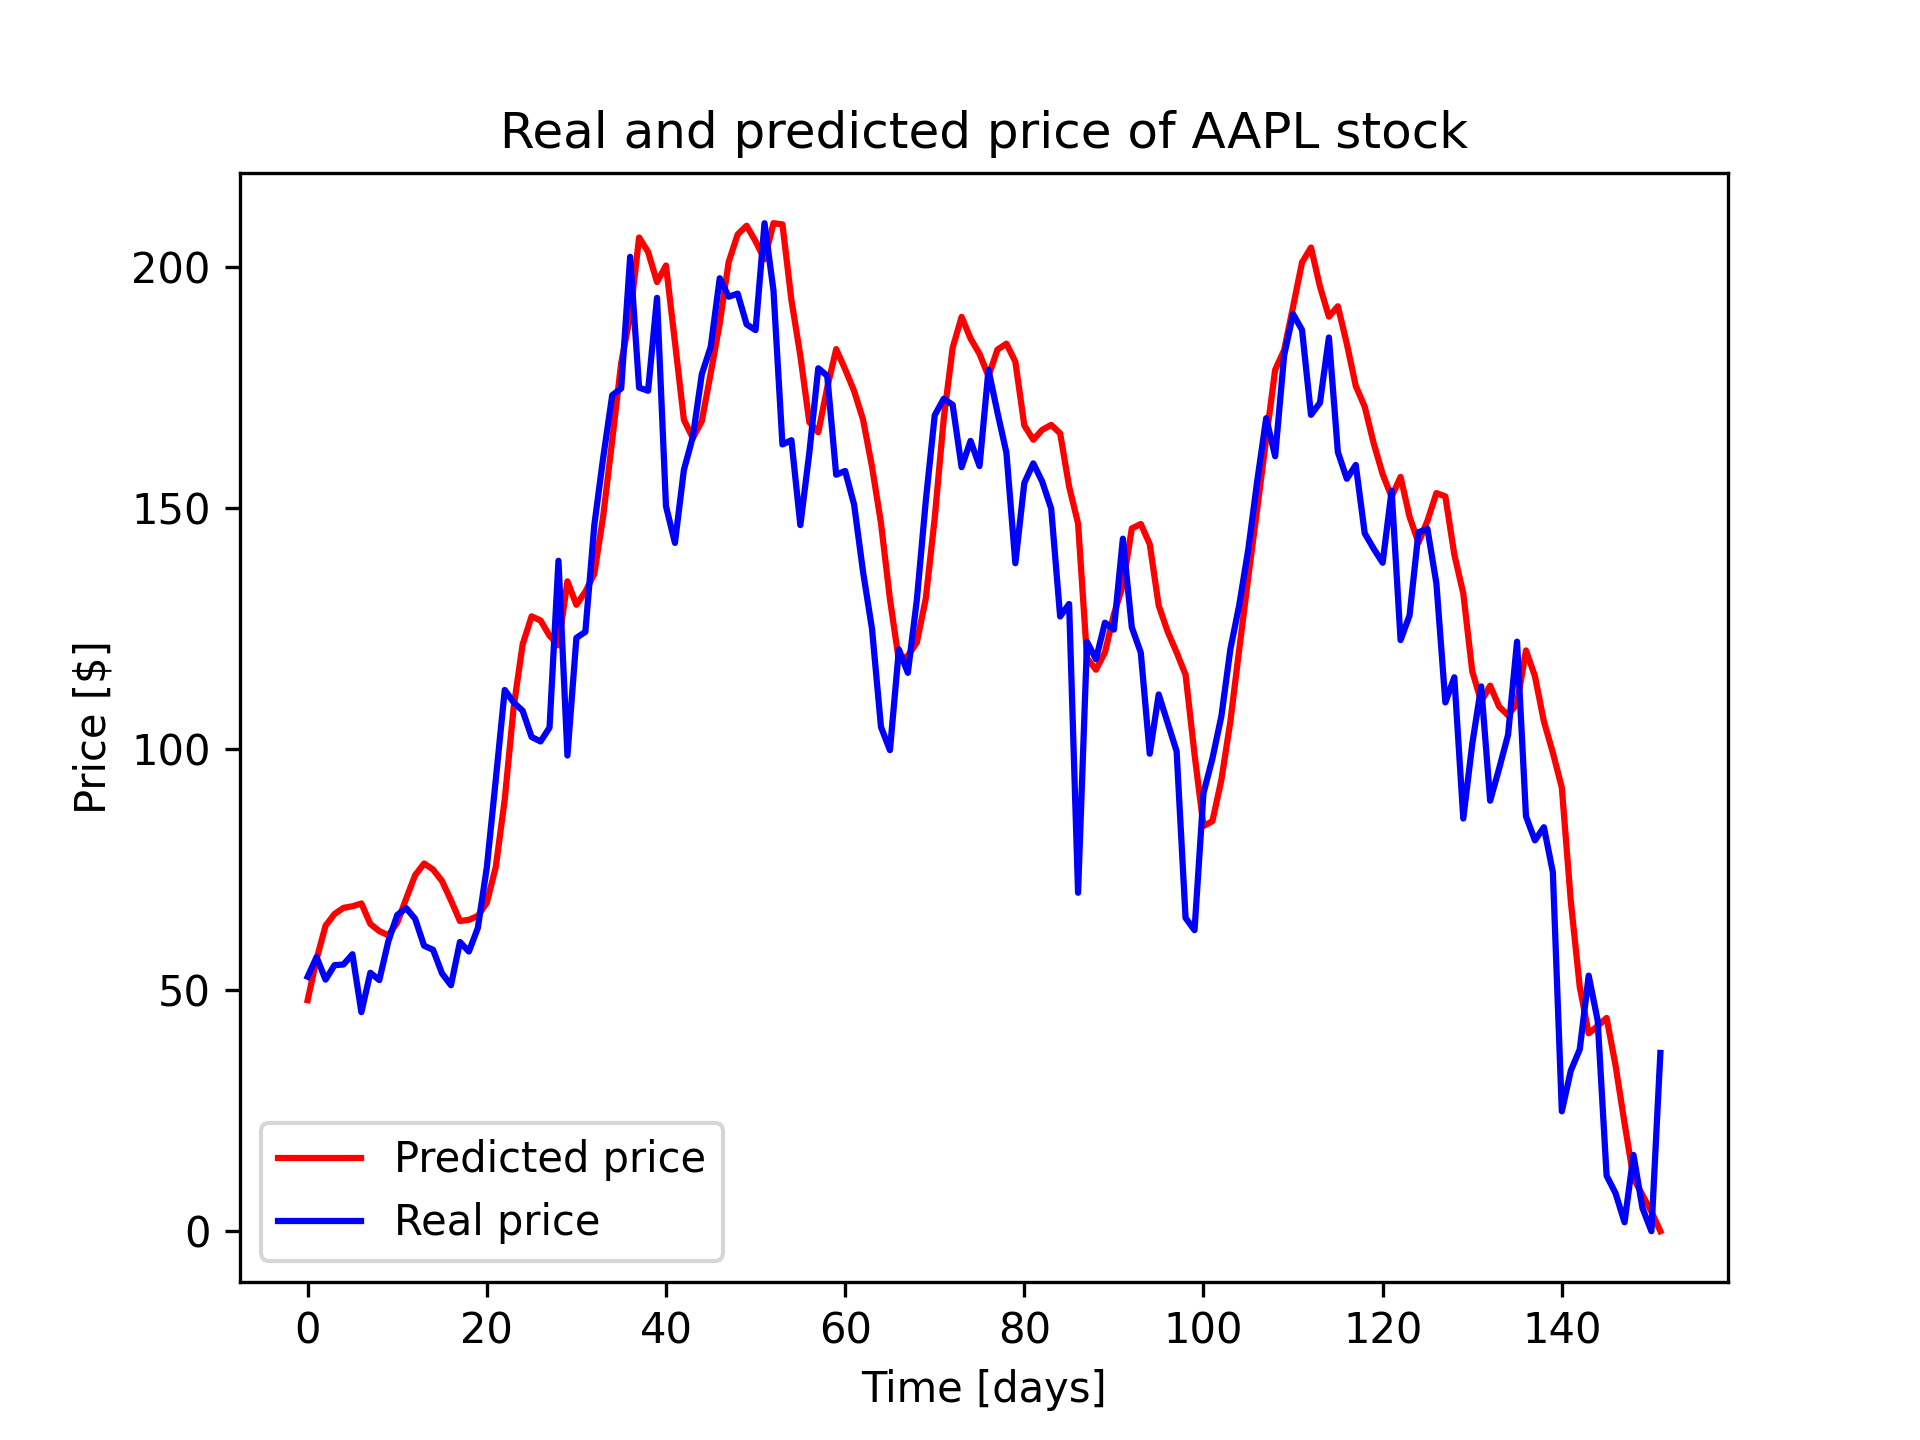
\includegraphics[width=0.5\textwidth]{./graf/model9/AAPL.png}
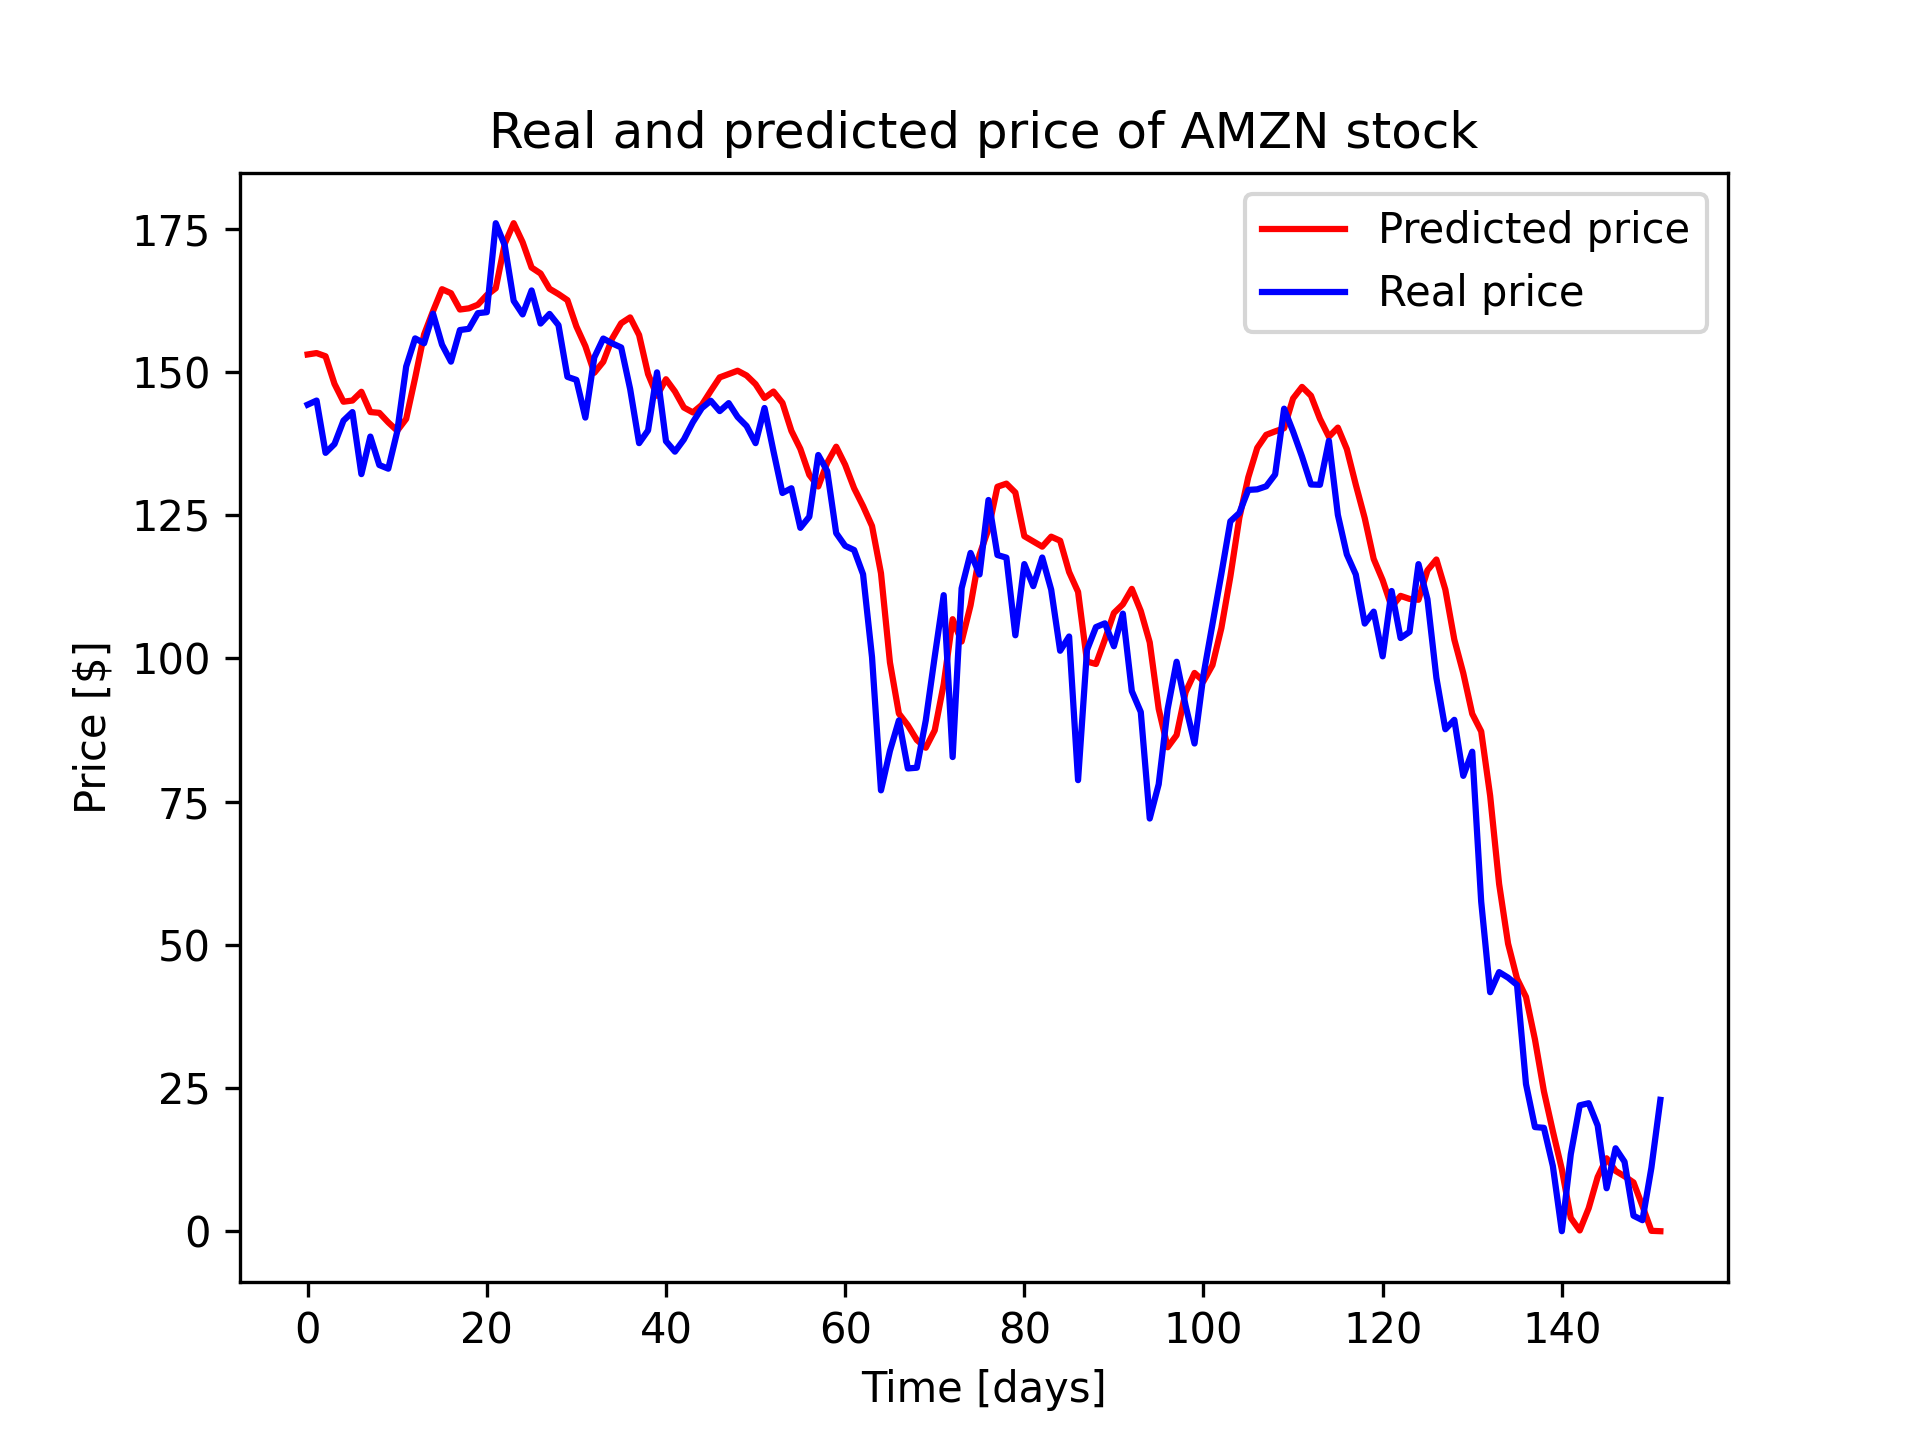
\includegraphics[width=0.5\textwidth]{./graf/model9/AMZN.png}
\includegraphics[width=0.5\textwidth]{./graf/model9/GOOGL.png}
\includegraphics[width=0.5\textwidth]{./graf/model9/LYFT.png}
\includegraphics[width=0.5\textwidth]{./graf/model9/NVDA.png}
\includegraphics[width=0.5\textwidth]{./graf/model9/TSLA.png}
\caption{Real and predicted prices of the ninth model.}
\label{fig:label}
\end{figure} 

\clearpage
\subsection{Comparison of models 1-9}
Different conclusions can be drawn when analyzing the results, depending on whether the analysis is graphical or analytical. Comparing the graphs, it can be concluded that the later models (5, 6) are better than the others. The first models, especially, look worse (1, 2, 3). However, analyzing the root-mean-square errors and losses, the first model appears to be the best, and the higher the model number, the worse its accuracy.
The important thing is that models can be evaluated in many different ways (for example considering accuracy, speed, or performance) and should be compared against different criteria. Both graph analysis and error analysis are of great value.
Many generated graphs and the presented analytical data confirm that the presented tool makes learning more accessible and allows one to become familiar with the operation and behavior of neural networks.
\clearpage
\setlength\tabcolsep{0pt}
\begin{table}
    \centering
    \caption{RMSE values for different companies and for different models.}
    \label{id:tab:wyniki}
    \begin{tabular*}{\linewidth}{@{\extracolsep{\fill}} cccccccccc }%{rrrrrrrrrr}
    \toprule
                 &                                     \multicolumn{8}{c}{Models}                                      \\
                 \cmidrule{2-10}
                 \cmidrule(r){4-6}\cmidrule(r){7-10}
        Companies &     Model 1 &   Model 2 & Model 3 & Model 4 & Model 5 & Model 6 & Model 7 & Model 8 & Model 9 \\
    \midrule
              AAPL  & 10.51& 8.91 & 10.38 & 8.9    & 8.45  & 9.21 & 8.82  & 12.85 & 11.89 \\
              AMZN  & 1.99 & 1.13 & 2.19  & 7.51   & 6.33  & 6.25 & 8.3   & 7.45  & 5.48 \\
              GOOGL & 4.94 & 6.08 & 7.8   & 5.31   & 7.81  & 9.55 & 6.91  & 9.33  & 8.89 \\
              LYFT  & 2.12 & 2.05 & 2.3   & 1.99   & 1.56  & 2.13 & 2.79  & 2.82  & 2.1 \\
              NVDA  & 4.15 & 4.73 & 6.12  & 6.67   & 6.94  & 8.78 & 7.46  & 10.22 & 8.84 \\
              TSLA  & 0.3  & 1.18 & 1.19  & 0.59   & 2.5   & 5.2  & 5.4   & 7.38  & 5.37 \\
              Mean value  & 4 & 4.01 & 4.99 & 5.16 & 5.6   & 6.86 & 6.61  & 8.34  & 7.1 \\
    \bottomrule
    \end{tabular*}
    \end{table}  
    